%% LyX 2.3.7 created this file.  For more info, see http://www.lyx.org/.
%% Do not edit unless you really know what you are doing.
\documentclass[english]{book}
\usepackage[latin9]{inputenc}
\usepackage[a4paper]{geometry}
\geometry{verbose,tmargin=2cm,bmargin=2cm,lmargin=1in,rmargin=1.5cm}
\setcounter{secnumdepth}{3}
\setcounter{tocdepth}{3}
\usepackage{verbatim}
\usepackage{fancybox}
\usepackage{calc}
\usepackage{textcomp}
\usepackage{amsmath}
\usepackage{amssymb}
\usepackage{makeidx}
\makeindex
\usepackage{graphicx}
\usepackage{esint}

\makeatletter

%%%%%%%%%%%%%%%%%%%%%%%%%%%%%% LyX specific LaTeX commands.
\DeclareFontEncoding{LGR}{}{}
\DeclareRobustCommand{\greektext}{%
  \fontencoding{LGR}\selectfont\def\encodingdefault{LGR}}
\DeclareRobustCommand{\textgreek}[1]{\leavevmode{\greektext #1}}
\ProvideTextCommand{\~}{LGR}[1]{\char126#1}

\DeclareTextSymbolDefault{\textquotedbl}{T1}
%% Because html converters don't know tabularnewline
\providecommand{\tabularnewline}{\\}
%% A simple dot to overcome graphicx limitations
\newcommand{\lyxdot}{.}


%%%%%%%%%%%%%%%%%%%%%%%%%%%%%% Textclass specific LaTeX commands.
\@ifundefined{lettrine}{\usepackage{lettrine}}{}
\newcommand{\lyxaddress}[1]{
	\par {\raggedright #1
	\vspace{1.4em}
	\noindent\par}
}
\providecommand*{\strong}[1]{\textbf{#1}}

%%%%%%%%%%%%%%%%%%%%%%%%%%%%%% User specified LaTeX commands.
\usepackage[style=authoryear,backend=biber,refsection=part]{biblatex}
\addbibresource{Bibliography/CC/P-Graphs/4e/introduction.bib}
\addbibresource{Bibliography/CC/P-Graphs/4e/kinematics.bib}
\addbibresource{Bibliography/CC/P-Graphs/4e/lawsofmotion.bib}
\addbibresource{Bibliography/CC/P-Graphs/4e/energyconservation.bib}
\addbibresource{Bibliography/CC/P-Graphs/4e/shm.bib}
\addbibresource{Bibliography/CC/P-Graphs/4e/currentelectricity.bib}
\addbibresource{Bibliography/CC/P-Graphs/4e/lattice.bib}

\makeatother

\usepackage{babel}
\begin{document}
\title{A Complete Course in Physics ( Graphs ) - 5th Edition}
\author{Manas Kalia and Rajat Kalia}
\date{7 December , 2023}
\maketitle

\lyxaddress{764 41-A , Chd}

\tableofcontents{}

\part*{Initiation}

\chapter*{Preface}

This book is a plethora on Graphs. Usually this topic , i.e. GRAPHS
is studied with lots of hype in Coachings, but unfortunately , not
lots of good study material is available. This book fulfills a long
felt need by students and teachers for an authorative text on graphs.

This book contains only reviewed material already being used by millions
of professors in universities. Reason being, to keep the correctness
and homogeneity intact.

The source of most graphs in this book is either internet or already
published books , proper bibliography has been added to give credit
to seemingly original creators. 

\chapter*{Acknowledgements}

I would like to thank my son Manas for his love and support. Moreover
, to my father for the day to day needs.

\part*{Prelims}

\part{Introduction}

\chapter{Theory }

\section{Introduction \cite{www.lhup.edu}}

A graph is an accurate pictorial representation of data. The accuracy
of data in physics requires that graphs be made on good quality graph
paper. Nearly all graphs in physics are smooth line graphs; broken
line (connect the dots) graphs and bar graphs are seldom appropriate. 

The style and format of a graph will depend upon its intended purpose.
Three types are common in physics

1. PICTORIAL GRAPHS. These are the kind found in mathematics and physics
textbooks. Their purpose is to simply and clearly illustrate a mathematical
relation. No attempt is made to show data points or errors on such
a graph.

2. DISPLAY GRAPHS. These present the data from an experiment. They
are found in laboratory reports, research journals, and sometimes
in textbooks. They show the data points as well as a smooth line representing
the mathematical relation.

3. COMPUTATIONAL GRAPHS. These are drawn for the purpose of extracting
a numerical result from the data. An example is the calculation of
the slope of a straight line graph, or its intercepts.

\section{\index{Elements of a good Graph}Elements of a good Graph}

Certain informational and stylistic features are required in all graphs:

1. The graph must have a descriptive title or caption, clearly stating
what the graph illustrates.

2. Data points are plotted as small dots with a sharp pencil, or as
pinpricks. Some method should be used to emphasize the location of
the points, for example, a neat circle drawn around each point.

\doublebox{\begin{minipage}[t]{0.72\columnwidth}%
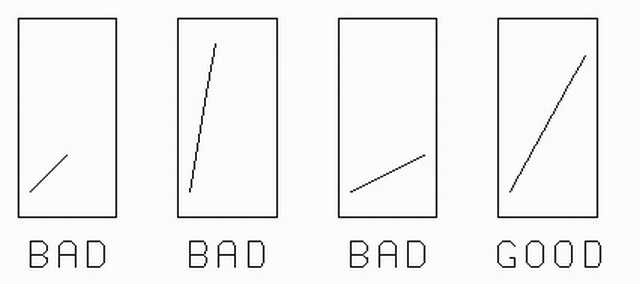
\includegraphics[scale=0.5]{Images/CC/P-Graphs/5e/Images/Introduction/G01}

Figure :Good and bad choices of geometric slope of a graph.%
\end{minipage}}

3. Curves drawn through the points should be smooth (use \footnote{A French curve is a template usually made from metal, wood or plastic
composed of many different curves. It is used in manual drafting to
draw smooth curves of varying radii. The shapes are segments of the
Euler spiral or clothoid curve. The curve is placed on the drawing
material, and a pencil, knife or other implement is traced around
its curves to produce the desired result.

Modern computer-aided design (CAD) systems use vector-based graphics
to achieve a precise radius, so no template is required. Digital computers
can also be used to generate a set of coordinates that accurately
describe an arbitrary curve, and the points can be connected with
line segments to approximate the curve with a high degree of accuracy.
Some computer-graphics systems make use of B�zier curves, which allow
a curve to be bent in real time on a display screen to follow a set
of coordinates, much in the way a French curve would be placed on
a set of three or four points on paper.} French curves if your hand is not steady). The curve should stand
out clearly.

4. Choose scales that are convenient to plot and easy to read.

5. Choose scales such that the graph occupies most of the page. The
two scales need not have the same size units. Also, the scales need
not begin at zero.

6. Indicate the name, letter symbol and units of each variable plotted
on each axis.

7. All text (title, labels, etc.) should be printed.

PHYSICAL SLOPE AND GEOMETRIC SLOPE

Slope. When textbooks refer to the \textquotedbl slope\textquotedbl{}
of a plotted graph line we mean the \textquotedbl physical slope\textquotedbl{}

physical slope = $\dfrac{\text{\textgreek{D}}y}{\text{\textgreek{D}}x}$ 

where \textgreek{D}y and \textgreek{D}x are expressed in the physical
units of the x and y axes. This slope has physical significance in
describing the physical data.

Geometric slope. A line which makes a 45� angle with an axis will
not necessarily have a physical slope of size 1. Some authors introduce
the term \textquotedbl geometric slope\textquotedbl{} to describe
the tilt of the line on the page. This is a ratio of lengths of the
legs of the triangle, without reference to the units plotted on the
axes.

There is seldom (probably never) any need to calculate the geometric
slope of a line on a graph. The idea is only useful when describing
the appearance of the graph on the page. One rule of graph construction
states that the graph should occupy most of the page. For square graph
paper this suggests a geometric slope of 45�. See Fig for examples
of good and bad choices of geometric slope.

THE APPEARANCE OF THE GRAPH

\doublebox{\begin{minipage}[t]{0.72\columnwidth}%
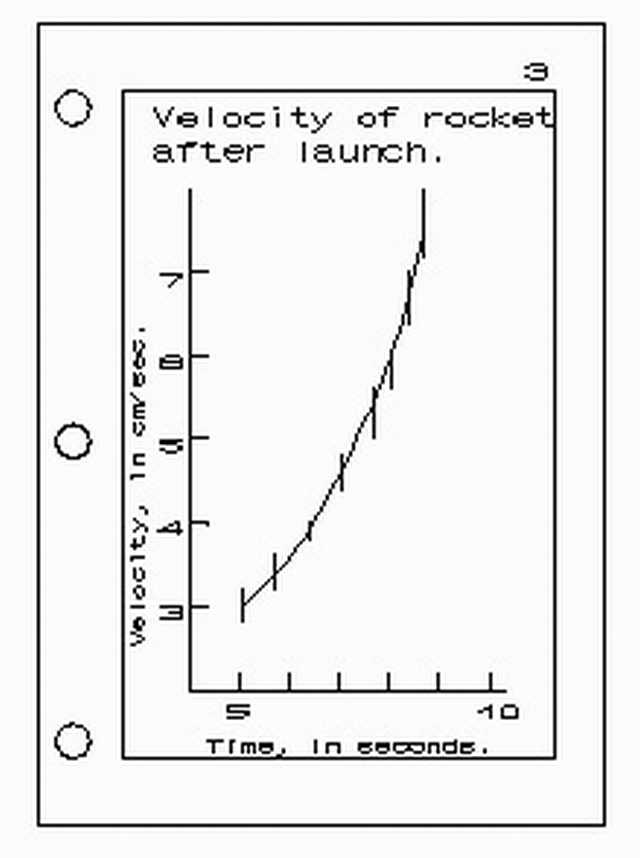
\includegraphics[scale=0.5]{Images/CC/P-Graphs/5e/Images/Introduction/G02}

Figure : Elements of a graph.%
\end{minipage}}

Use quality graph paper, size 8.5 by 11 inches only.

The left margin is largest, for binding or stapling.

Nothing should be in the white margins except a page number. Axes,
lettering and labeling should all be within the printed grid area.
{[}The grid lines serve as guide lines for neat, uniform printed lettering.{]}

The title must be descriptive.

Both axes are labeled with the full name of the quantity (not merely
its symbol), and its units.

The plotted points and curve should occupy most (more than half) of
the area of the graph paper.

Sometimes a small sketch of the experimental situation may be included,
located where it will not confuse the interpretation of the graph.
In the same manner an equation, or short explanatory comment, may
be included.

\section{\index{Graphical Representation of Uncertainties}Graphical Representation
of Uncertainties}

Display graphs and computational graphs should clearly show the size
of the experimental uncertainties (errors) in each plotted point.
There are several conventional ways to do this, the commonest being
the use of error bars illustrated below:

\doublebox{\begin{minipage}[t]{0.72\columnwidth}%
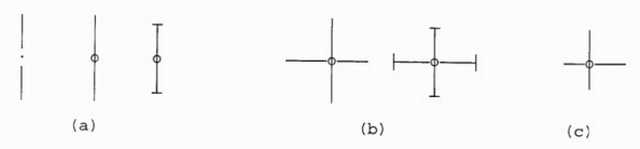
\includegraphics[scale=0.5]{Images/CC/P-Graphs/4.1e/Images/Introduction/G03}

Figure : Various styles of error bars. %
\end{minipage}}

The plotted point is represented as a dot, and the range of uncertainty
is shown by the extent of the bars on either side. The types shown
in (a) are suitable where the error is entirely in one variable, or
where the errors in both variables have been lumped together. The
types shown in (b) are preferred where it is necessary to show the
error in each variable explicitly.

When the uncertainties have a symmetric distribution about the mean,
the error bars extend equally on either side of the points. If the
data distributions are not symmetric, the plotted points will not
be centrally located in the range of uncertainty and the error bars
might look like those in Figure. part (c).

Error bars may not be necessary when the data points are so numerous
that their scatter is clearly shows the uncertainty. In these cases
error bars would clutter the graph making it difficult to interpret.
Another situation where error bars are inappropriate is when the scale
of the graph is such that the bars would be very small. In this case,
it may be possible to indicate the uncertainty by the size of the
circle or rectangle surrounding each point.

\section{Curve Fitting\index{Curve Fitting}}

The curve drawn through plotted data need not pass exactly through
every data point. But usually the curve should pass within the uncertainty
range of each point, that is, within the error bars, if the bars represent
limits of error.

One principle of curve fitting is also a fundamental rule of science
itself:

Assume the simplest relation consistent with the data. We are not
justified in assuming a more complex relation than can be demonstrated
by the data. If a curve were drawn with detail smaller than the data
uncertainty, that detail would be only a guess.

This rule of simplicity may also be expressed mathematically. The
mathematical relations encountered in physics may often be represented
by power series such as

$y=A+Bx+Cx^{2}+Dx^{3}+Ex^{4}+...$

where A, B, C, ... are constants.

For very \textquotedbl wiggly\textquotedbl{} curves, many terms of
this equation, including high powers of x, might be required to express
the equation of the relation. The simplest relations are those which
contain the smallest powers of x. The simplest relations of all are

y = a or y = a + bx

which describe straight lines. Many relations in physics are, fortunately,
of this form. Others only include the $x^{2}$ term, describing a
parabolic curve. Note that double valued curves, sometimes encountered
in physics, cannot be represented by Equation. 

When sizable amounts of data are taken, standard mathematical methods
are available which generate the equation of the simplest curve which
statistically \textquotedbl best fits\textquotedbl{} the data.

The student may wonder how one can be certain that the curve fitted
to the data is the \textquotedbl correct\textquotedbl{} curve. The
answer is that relations are never known with certainty. The uncertainty
of available data always limits the certainty of the results. Someday
someone may obtain more accurate data and be able to show that the
old relations are slightly incorrect, and provide us with better ones.
As data improves, so does our understanding of relations\textemdash this
is the way of scientific progress. But we never should claim to know
a relation better than the data allows.

\section{\index{Uncertainty in a Slope}Uncertainty in a Slope}

One use of a computational graph is to determine the slope of a straight
line. This is illustrated in Figure. Eight data points are shown with
error bars on each. If these bars represent maximum error, any line
drawn to represent this data should pass within all bars.

If the error bars represent error estimates smaller than the maximum
(average deviation, standard deviation, etc.), then the fitted curve
need not pass within all of the error bars, just most of them.

\doublebox{\begin{minipage}[t]{0.72\columnwidth}%
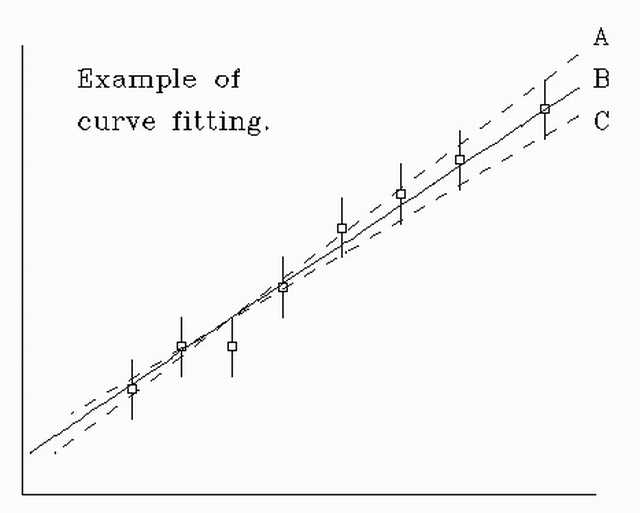
\includegraphics[scale=0.5]{Images/CC/P-Graphs/5e/Images/Introduction/G04}

Figure : Fitting a curve.%
\end{minipage}}

Even a simple \textquotedbl manual\textquotedbl{} curve fit with
a ruler can reveal the uncertainties in the slope resulting from uncertainties
in the data. Figure. illustrates this process.

The dotted lines A and C fall within the error bars, and represent
the maximum and minimum slope one could justify from this data. The
\textquotedbl best\textquotedbl{} value of slope might be that of
solid line B.

The third point from the left seems to limit the slope the most, and
would appear to be \textquotedbl suspect.\textquotedbl{} But one
ought not to \textquotedbl throw it out\textquotedbl{} without better
reason, based on further investigation.

\section{\index{Graphical Analysis of Data}Graphical Analysis of Data}

Graphs can be a valuable tool for determining or verifying functional
relations between variables. Many special types of graph paper are
available for handling the most frequently encountered relations.
You are probably already familiar with linear graph paper and polar
coordinate paper.

You may have purchased a packet of graph paper for this course. It
includes samples of graph papers you will use in this course, and
a few other types. As you read the material below, examine the corresponding
papers from your packet.

LINEAR RELATIONS are those which satisfy the equation

y = mx + b

where the variables are x and y, and m and b are constants. When y
is plotted against x on ordinary Cartesian (linear) graph paper, the
points fall on a straight line with slope m and a y-intercept b, as
shown in Fig. 1.5.

The slope of an experimental relation is often physically significant.
It is obtained by choosing two well-separated points on the line (x$_{1}$,
y$_{1}$) and (x$_{2}$, y$_{2}$). From Eq. 7-3:

$y_{1}=mx_{1}+b$

and $y_{2}=mx_{2}+b$

Subtract the first from the second.

$(y_{2}-y_{1})=m(x_{2}-x_{1})$ .

\doublebox{\begin{minipage}[t]{0.72\columnwidth}%
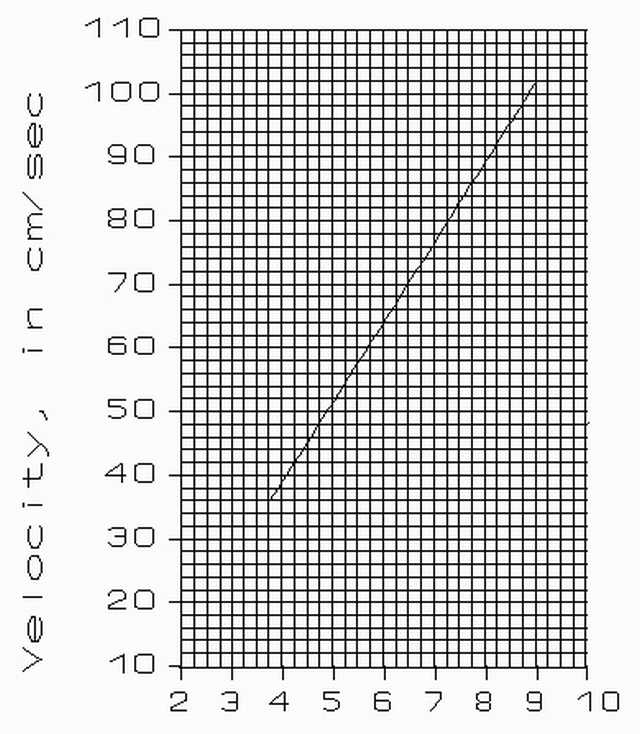
\includegraphics[scale=0.5]{Images/CC/P-Graphs/5e/Images/Introduction/G06}

Figure : Measuring a slope on linear graph paper. %
\end{minipage}}

Therefore,

m = $\dfrac{y_{2}-y_{1}}{x_{2}-x_{1}}$ = $\dfrac{\text{\textgreek{D}}y}{\text{\textgreek{D}}x}$

The slope of a straight line is a ratio of the \textquotedbl lengths\textquotedbl{}
of two legs of a right triangle constructed with the legs parallel
to the graph axes and with the graph line along the hypotenuse. Figure.
illustrates this, the slope being \textgreek{D}y/\textgreek{D}x.

So far this discussion has been strictly mathematical. Now let's consider
a fairly realistic physical example. Figure. shows the curve from
measurements of the velocity of a moving body as a function of time.

If we use letters v for velocity and t for time, we'd expect this
curve to be described by the relation:

v = v$_{o}$ + at

Here the constant a (acceleration) is the slope of the line, while
v$_{o}$ plays the role of b in Equation. These two constants are
physically significant, and we wish to find their values from the
graph.

We choose two points on the line at t = 4.25 and 8.75, with corresponding
values of velocity: 42 cm/s and 98 cm/s. Mark these points on Figure.
, to confirm these values. The slope of the line is therefore:

$a=\dfrac{(98cm/s-42cm/s)}{8.75s-4.25s}=\dfrac{56}{4.5}\;cm/s^{2}=56/4.5\;cm/s^{2}=12.44cm/s^{2}$

When calculating this ratio do not use ruler-measured lengths. The
lengths are expressed in the units marked on the graph axes. The calculated
slope is therefore independent of the particular choice of units,
of the way you choose to label the graph scale divisions, and is also
independent of the size of the graph paper.

INTERCEPTS: The values of the intercepts are often physically significant.
They can be simply read from the graph\textemdash if the $x=0$ and
$y=0$ axes happen to be within the graph's boundaries. In the equation
y = mx + b, the y intercept is b.

The v intercept of Figure. is the value of v when t = 0. It has the
same units and dimensions as y. If, as in this case, the v intercept
does not lie within the area of the graph, it may be calculated using
the slope and one value taken from a point on the fitted line. Take
the point v = 98 cm/s when t = 8.75 sec.

v = v$_{o}$ + at , in our case, v = v$_{o}$ + 12.44 t

so,

v = v$_{o}$ - 12.44 t = 98 - 12.44(8.75) = -10.89 cm/s A check of
the graph, Figure. , shows that this looks reasonable.

STRAIGHTENING A CURVE. When it is possible to convert an experimental
relation to a straight line graph it is usually useful to do so. Look
for such opportunities. For example, when studying gases at constant
temperature we find that

PV = C

where P is pressure, V is the gas volume and C is constant. The graph
of P vs. V is a branch of an hyperbola. But if we graph P vs. 1/V,
or V vs. 1/P, the data would fall on a straight line.

$P=\left(\dfrac{1}{V}\right)C$

One reason for doing this is that it is easier to fit the experimental
data with a ruler-drawn straight line, than to draw the best hyperbola
on a PV graph. Another advantage is that the P vs. 1/V graph has a
slope

$C=\dfrac{\triangle P}{\triangle\left(\dfrac{1}{V}\right)}$

Therefore the constant C is easily determined from the straight line.
This constant was not evident, nor was it easy to determine from the
PV graph!

Inexpensive electronic calculators make it so easy to manipulate data
that there is no good excuse to pass up an opportunity to \textquotedbl linearize\textquotedbl{}
experimental graphs.

\section{EXERCISES.}

In each case state how you could plot (x,y) data on linear paper to
obtain a straight line graph. What quantity in the equation is determinable
from the slope of the straight line? What quantity is determinable
from an intercept?

(1.1) x (y + 1) = 3

(1.2) 1/x + 1/y = 5

(1.3) $y=Ae^{-x}$

(1.4) $y=\surd(A-x)$

(1.5) $y^{2}+x^{2}=7$

\chapter{\index{Common Graph Forms in Physics}Common Graph Forms in Physics}

Working with graphs \textendash{} interpreting, creating, and employing
\textendash{} is an essential skill in the sciences, and especially
in physics where relationships need to be derived. As an introductory
physics student you should be familiar with the typical forms of graphs
that appear in physics. Below are a number of typical physical relationships
exhibited graphically using standard X-Y coordinates (e.g., no logarithmic,
power, trigonometric, or inverse plots, etc.). Study the forms of
the graphs carefully, and be prepared to use the program Graphical
Analysis to formulate relationships between variables by using appropriate
curve-fitting strategies. Note that all non-linear forms of graphs
can be made to appear linear by \textquotedblleft linearizing\textquotedblright{}
the data. Linearization consists of such things as plotting X versus
Y$^{2}$ or X versus 1/Y or Y versus log (X), etc. Note: While a 5th
order polynomial might give you a better fit to the data, it might
not represent the simplest model. 

\section{\index{Linear Relationship}Linear Relationship}

What happens if you get a graph of data that looks like this? How
does one relate the X variable to the Y variable? It\textquoteright s
simple, Y = A + BX where B is the slope of the line and A is the Y-intercept.
This is characteristic of Newton\textquoteright s second law of motion
and of Charles\textquoteright{} law: 

F= ma 

P/T = const. 

\doublebox{\begin{minipage}[t]{0.72\columnwidth}%
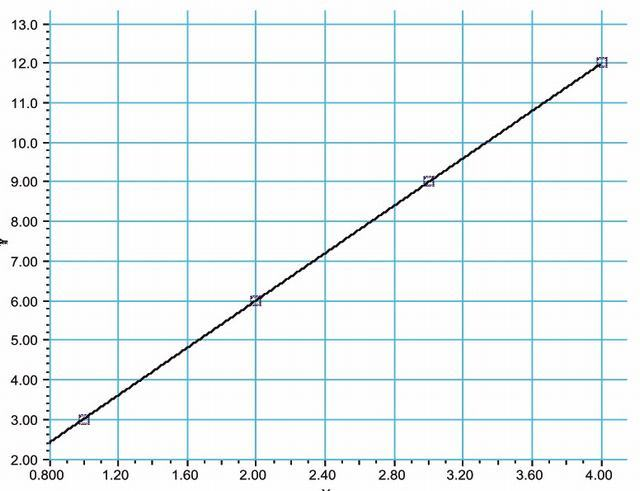
\includegraphics[scale=0.5]{Images/CC/P-Graphs/5e/Images/Kinematics/graph1_cgf}%
\end{minipage}}

\section{\index{Inverse Relationship}Inverse Relationship}

This might be a graph of the pressure and temperature for a changing
volume constant temperature gas. How would you find this relationship
short of using a computer package? The answer is to simplify the plot
by manipulating the data. Plot the Y variable versus the inverse of
the X variable. The graph becomes a straight line. The resulting formula
will be Y = A/X or XY = A. This is typical of Boyle\textquoteright s
law: 

PV = const

\doublebox{\begin{minipage}[t]{0.72\columnwidth}%
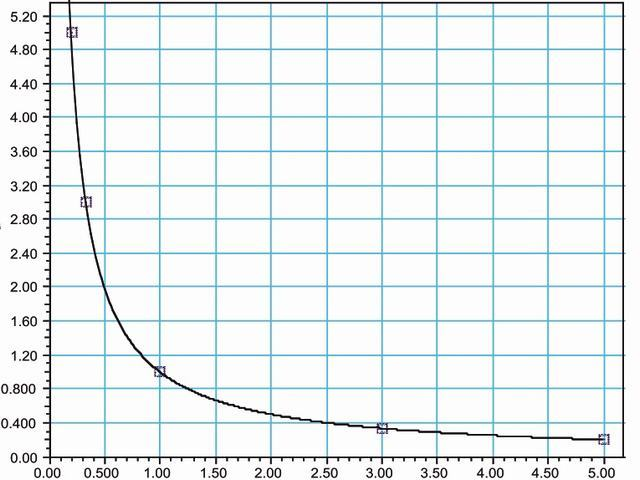
\includegraphics[scale=0.5]{Images/CC/P-Graphs/5e/Images/Kinematics/graph2_cgf}%
\end{minipage}}

\section{\index{Inverse-Square Relationship}Inverse-Square Relationship}

Of the form Y = A/X$^{2}$. Characteristic of Newton\textquoteright s
law of universal gravitation, and the electrostatic force law: 

$F=\dfrac{Gm_{1}m_{2}}{r^{2}}$

$F=\dfrac{kq_{1}q_{2}}{r^{2}}$

\doublebox{\begin{minipage}[t]{0.72\columnwidth}%
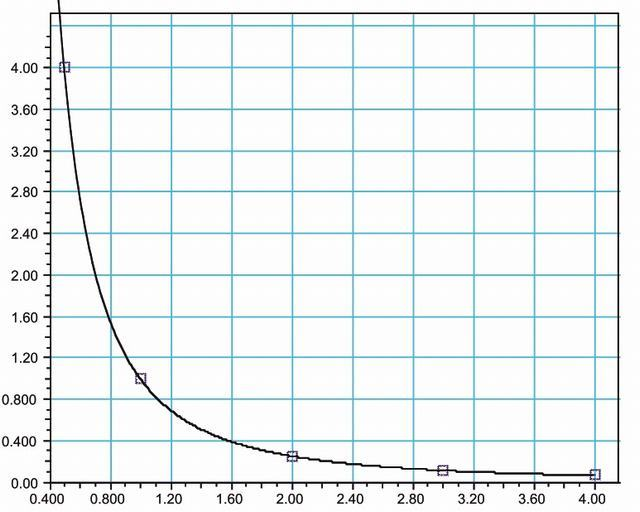
\includegraphics[scale=0.5]{Images/CC/P-Graphs/4.1e/Images/Kinematics/graph3_cgf}%
\end{minipage}}

In the latter two examples above there are only subtle differences
in form. Many common graph forms in physics appear quite similar.
Only by looking at the \textquotedblleft RMSE\textquotedblright{}
(root mean square error provided in Graphical Analysis) can one conclude
whether one fit is better than another. The better fit is the one
with the smaller RMSE. See below for more examples of common graph
forms in physics. 

\section{\index{Double-Inverse Relationship}Double-Inverse Relationship}

Of the form 1/Y = 1/X + 1/A. Most readily identified by the presence
of an asymptotic boundary (y = A) within the graph. This form is characteristic
of the thin lens and parallel resistance formulas. 

$\dfrac{1}{f}=\dfrac{1}{d_{i}}+\dfrac{1}{d_{o}}$

and 

$\dfrac{1}{R_{t}}=\dfrac{1}{R_{1}}+\dfrac{1}{R_{2}}$

\doublebox{\begin{minipage}[t]{0.72\columnwidth}%
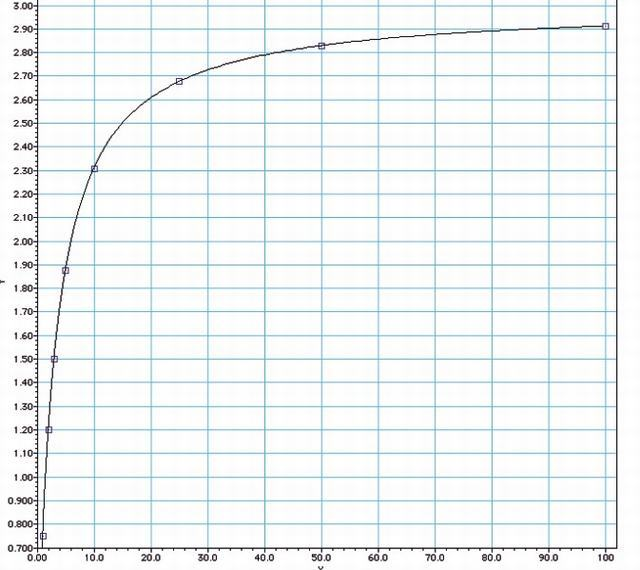
\includegraphics[scale=0.5]{Images/CC/P-Graphs/5e/Images/Kinematics/graph4_cgf}%
\end{minipage}}

\section{\index{Power Relationship}Power Relationship}

Top opening parabola. Of the form $Y=AX^{2}$. Typical of the distance-time
relationship: 

$d=\dfrac{1}{2}at^{2}$

\doublebox{\begin{minipage}[t]{0.72\columnwidth}%
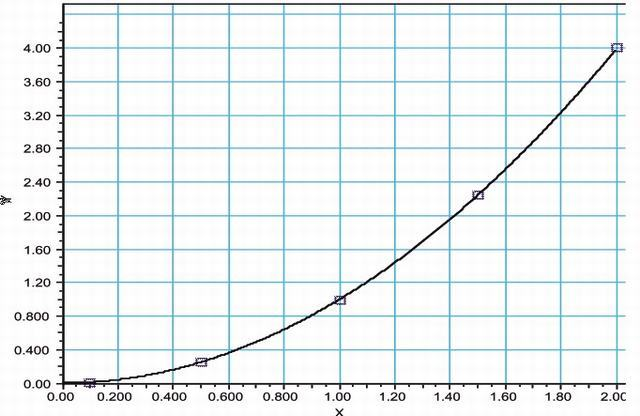
\includegraphics[scale=0.5]{Images/CC/P-Graphs/5e/Images/Kinematics/graph5_cgf}%
\end{minipage}}

\section{\index{Power Relationship 2}Power Relationship 2}

Side opening parabola. Of the form $Y^{2}=A_{1}X$ or $Y=A_{2}X^{1/2}$.
Typical of the simple pendulum relationship: $P^{2}=k_{1}l$ or $P=k_{2}\sqrt{l}$

\doublebox{\begin{minipage}[t]{0.72\columnwidth}%
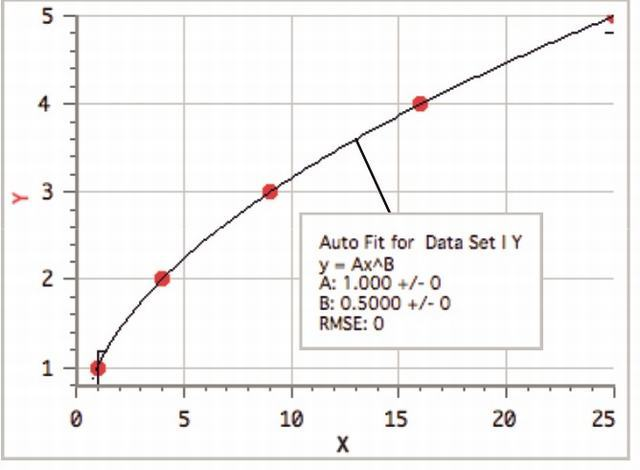
\includegraphics[scale=0.5]{Images/CC/P-Graphs/4.1e/Images/Kinematics/graph6_cgf}%
\end{minipage}}

\section{\index{Polynomial of Second Degree}Polynomial of Second Degree}

Of the form $Y=AX+BX^{2}$. Typical of the kinematics equation:

$d=v_{o}t+\dfrac{1}{2}at^{2}$

\doublebox{\begin{minipage}[t]{0.72\columnwidth}%
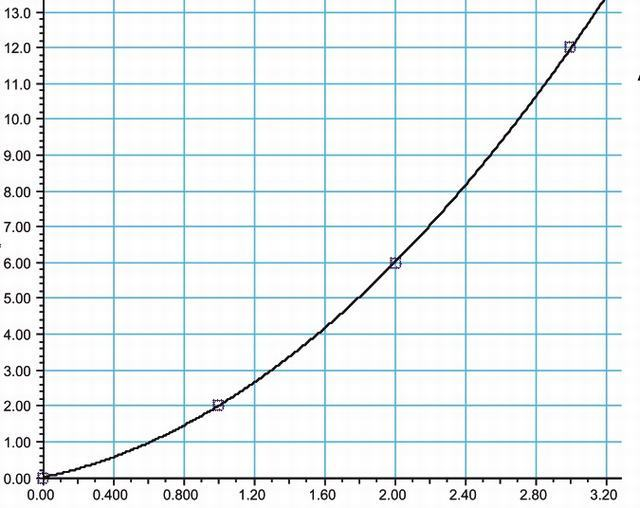
\includegraphics[scale=0.5]{Images/CC/P-Graphs/5e/Images/Kinematics/graph7_cgf}%
\end{minipage}}

\section{\index{Exponential Relationship}Exponential Relationship}

Of the form Y = A {*} exp(BX). Characteristic of exponential growth
or decay. Graph to left is exponential growth. The graph of exponential
decay would look not unlike that of the inverse relationship. Characteristic
of radioactive decay.

$N=Noe^{-\lambda t}$

\doublebox{\begin{minipage}[t]{0.72\columnwidth}%
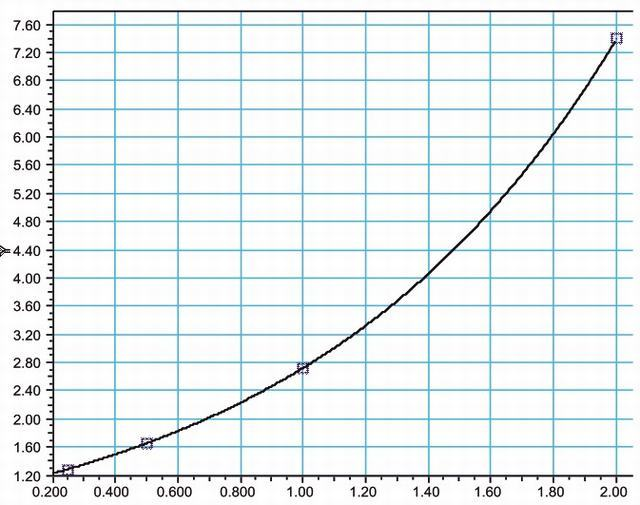
\includegraphics[scale=0.5]{Images/CC/P-Graphs/4.1e/Images/Kinematics/graph8_cgf}%
\end{minipage}}

\section{\index{Natural Log (LN) Relationship}Natural Log (LN) Relationship}

Of the form Y = A ln(BX). Characteristic of entropy change during
a free expansion: 

$S_{f}-S_{i}=nRln\left(V_{f}/V_{i}\right)$

\doublebox{\begin{minipage}[t]{0.72\columnwidth}%
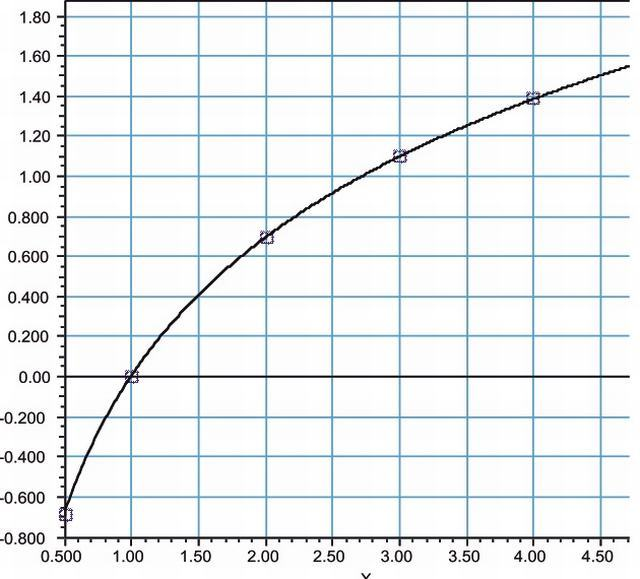
\includegraphics[scale=0.5]{Images/CC/P-Graphs/5e/Images/Kinematics/graph9_cgf}%
\end{minipage}}

\begin{comment}
\begin{btSect}[plain]{Bibliography/CC/P-Graphs/5e/introduction}
\btPrintCited
\end{btSect}
\end{comment}

\printbibliography

\part*{Mechanics}

\part{Kinematics}

\chapter{Abstract Introduction}

\doublebox{\begin{minipage}[t]{0.72\columnwidth}%
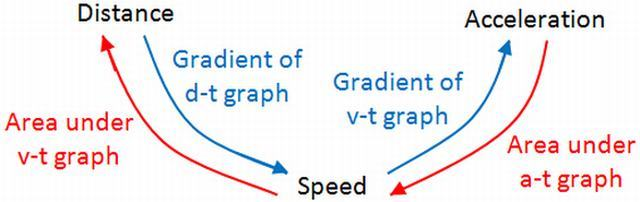
\includegraphics[scale=0.5]{Images/CC/P-Graphs/4.1e/Images/Kinematics/4791850}

Figure : Graphical Representation of what we are going to learn in
this chapter.%
\end{minipage}}

\doublebox{\begin{minipage}[t]{0.72\columnwidth}%
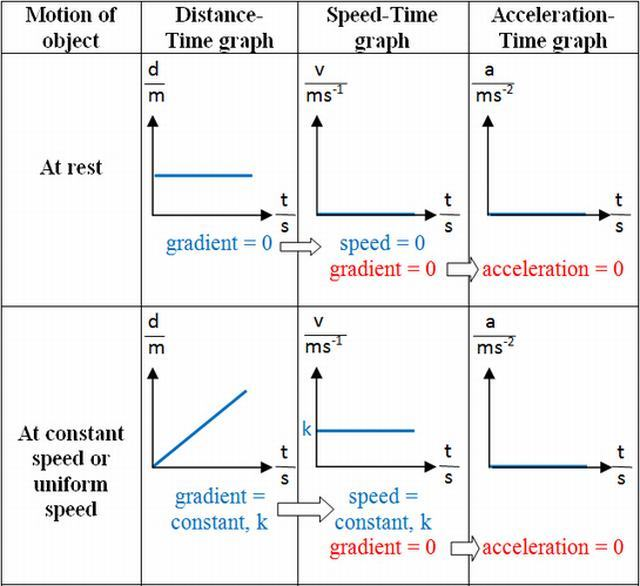
\includegraphics[scale=0.5]{Images/CC/P-Graphs/4.1e/Images/Kinematics/9327449}

Figure : Some Graphs%
\end{minipage}}

\doublebox{\begin{minipage}[t]{0.72\columnwidth}%
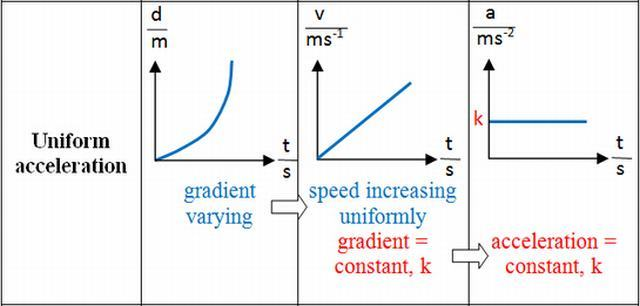
\includegraphics[scale=0.5]{Images/CC/P-Graphs/4.1e/Images/Kinematics/6331664}

Figure : Few more graphs%
\end{minipage}}

\doublebox{\begin{minipage}[t]{0.72\columnwidth}%
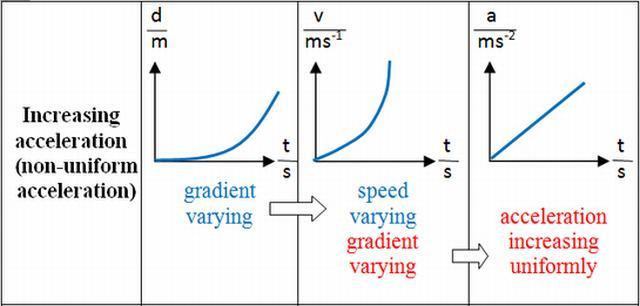
\includegraphics[scale=0.5]{Images/CC/P-Graphs/4.1e/Images/Kinematics/5128203}

Figure : Few more%
\end{minipage}}

\doublebox{\begin{minipage}[t]{0.72\columnwidth}%
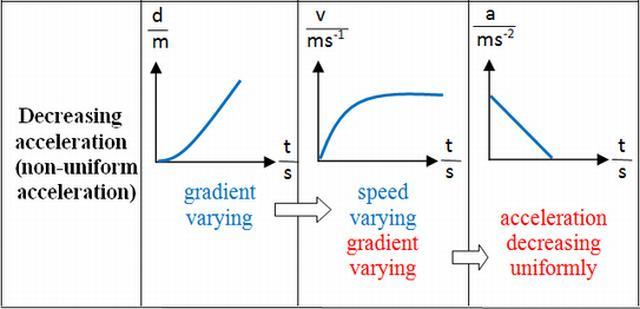
\includegraphics[scale=0.5]{Images/CC/P-Graphs/4.1e/Images/Kinematics/1922956}

Figure : Just last in this category.%
\end{minipage}}

If we have a high velocity, the graph has a steep slope. If we have
a low velocity the graph has a shallow slope (assuming the vertical
and horizontal scale of each graph is the same).

\doublebox{\begin{minipage}[t]{0.72\columnwidth}%
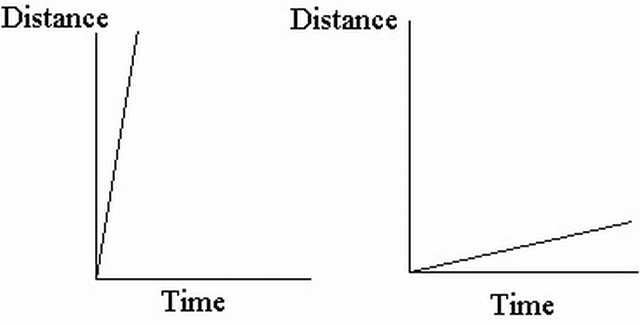
\includegraphics[scale=0.5]{Images/CC/P-Graphs/4.1e/Images/Kinematics/Image13}

Figure : Graph comparision of high speed vs low speed. {[} It may
be noted that in Distance-Time Graphs , the slope is Speed (Distance
and corresponding Speed both being Scalars), while in Displacement-Time
Graphs, the slope is velocity(Displacement and corresponding Velocity
both being Vectors).{]}%
\end{minipage}}

\doublebox{\begin{minipage}[t]{0.72\columnwidth}%
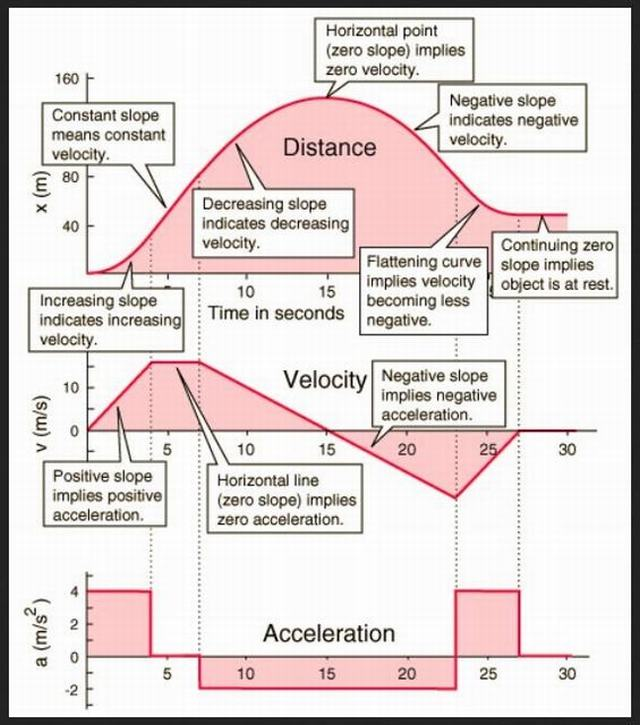
\includegraphics[scale=0.5]{Images/CC/P-Graphs/4.1e/Images/Kinematics/KinGraphSummary}

Figure : Graphical representation of the paradigms of this chapter.%
\end{minipage}}

\section{Displacement-Time Graph}

A displacement-time graph shows the positions of a moving object at
different times. Fig. shows the displacement-time graph of a car.
From time $t=0$ to $t=5$s , the car moves forward, and at $t=5$s
it has a displacement of 60 m. Then it remains stationary there for
5 s, and finally moves back to its starting position in another 5
s.\cite{www.hk-phy.org}

\doublebox{\begin{minipage}[t]{0.72\columnwidth}%
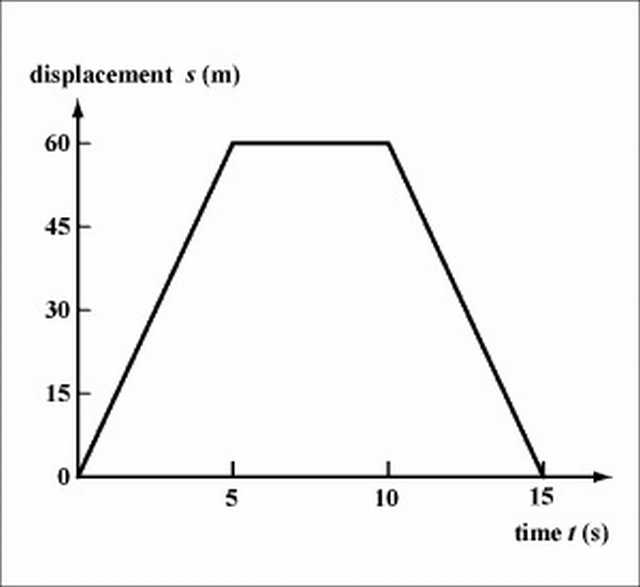
\includegraphics[scale=0.5]{Images/CC/P-Graphs/4.1e/Images/Kinematics/5-01}

Figure : Displacement-Time Graph of the problem being discussed.%
\end{minipage}}

The velocity of motion can be determined from the slope of the displacement-time
graph. The velocity of the car is $\dfrac{60}{5}=12m/s$ from t=0
to t=5s , it is zero (the car is at rest) from t=5s to t=10s and is
(0-60)/(15-10) from t=10s to t=15s. The negative slope in the last
5 s indicates that the car is moving backwards. Note that the slope
of the graph in each of the time intervals is a constant, showing
that the car is in a uniform motion (constant velocity) in each interval.
\begin{description}
\item [{Question}] : An object starts from rest and undergoes a positive,
constant acceleration for ten seconds, it then continues on with constant
velocity. Which of the following graphs correctly describes the situation?
\end{description}
\doublebox{\begin{minipage}[t]{0.72\columnwidth}%
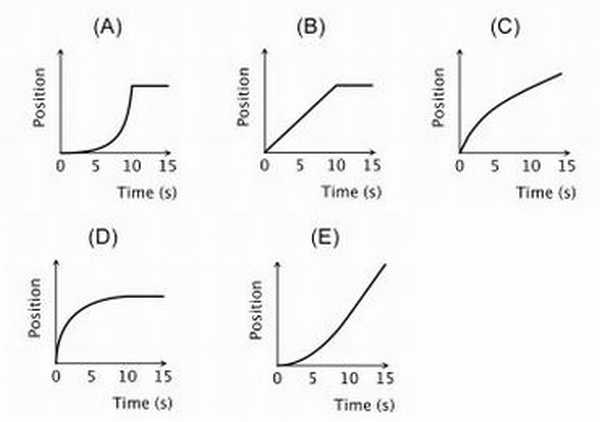
\includegraphics[scale=0.5]{Images/CC/P-Graphs/Common/Reduced/reviewkinematics/ImagesReduced/Tugk9-modified}%
\end{minipage}}

\cite{www.physport.org}

\section{Velocity-time graph}

A velocity-time graph shows the velocities of a moving object at different
times. Figure. shows three velocity-time graphs.\cite{www.hk-phy.org}

Fig. (a) represents motion at a constant velocity, the acceleration
is zero and thus the slope of the graph is zero. Fig. represents a
uniform acceleration given by

$a=\dfrac{v-u}{t}=\dfrac{6-0}{15}=0.4ms^{-2}$

,

This is represented by the slope of the velocity-time graph. Fig.
represents a uniform deceleration given by ,

$a=\dfrac{v-u}{t}=\dfrac{0-4}{15}\approx-0.27ms^{-2}$

which is also represented by the slope of the graph. The negative
slope indicates that the object decelerates. Note that the steeper
the slope, the larger is the magnitude of the acceleration.

\doublebox{\begin{minipage}[t]{0.72\columnwidth}%
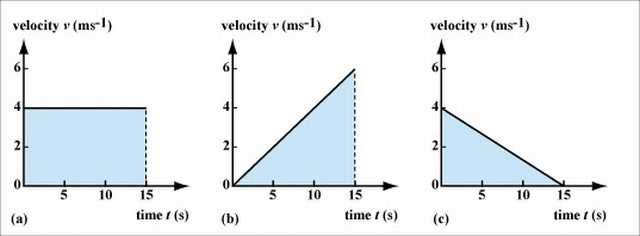
\includegraphics[scale=0.5]{Images/CC/P-Graphs/4.1e/Images/Kinematics/5-05}%
\end{minipage}}

Fig. For the uniform motion shown in Fig. (a), the displacement is
given by velocity $\times$ time = 4 $\times$ 15 = 60 . This is represented
by the area of the rectangle under the graph. In fact, for any velocity-time
graph, the displacement at a certain time can be calculated from the
area under the graph. Following this rule, we can work out the displacement
for an object in uniform acceleration or deceleration. For Fig. (b)
, the displacement is$6\times15/2=45m$ , while for Fig. (c), the
displacement is $4\times15/2=30m$

Fig. shows the velocity-time graph of an elevator moving upwards.
The elevator is initially at rest on the ground floor. It accelerates
from rest for 2.5 s, reaching a velocity of 1ms$^{-1}$, then it moves
at this constant velocity for 5 s, and finally decelerates to rest
in 2.5 s.

\doublebox{\begin{minipage}[t]{0.72\columnwidth}%
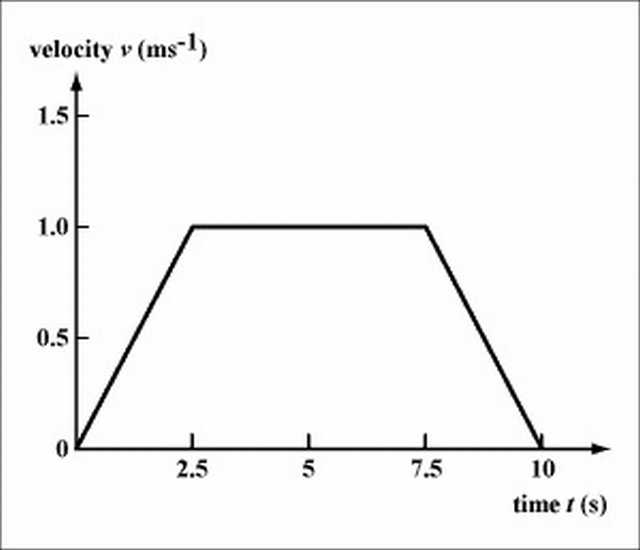
\includegraphics[scale=0.5]{Images/CC/P-Graphs/4.1e/Images/Kinematics/5-06}%
\end{minipage}}

The acceleration of the elevator at each time interval can be deduced
from the slope of the graph. In the first 2.5 s, the elevator accelerates
at 1/2.5=0.4ms$^{-2}$ . The acceleration is zero for the next 5 s,
and in the last 5 s the elevator decelerates at(0-1)/(10-7.5)=-0.4ms$^{-2}$
to rest (the negative slope indicates a deceleration). Note that for
the whole trip, the elevator is going upwards.

The total displacement can be calculated from the area under the graph.
In this example, the total displacement of the elevator is the area
of the trapezium under the graph, i.e., total displacement =(5+10)$\times$1/2=7.5m.

\section{Acceleration-time graph}

Fig. An acceleration-time graph shows the accelerations of a moving
object at different times. Fig. shows the acceleration-time graph
constructed from the velocity-time graph in Fig. . It can be seen
that during the first 2.5 s and the last 2.5 s, the elevator is moving
with a constant acceleration and deceleration respectively, and in
between it moves at a constant velocity (zero acceleration).

\doublebox{\begin{minipage}[t]{0.72\columnwidth}%
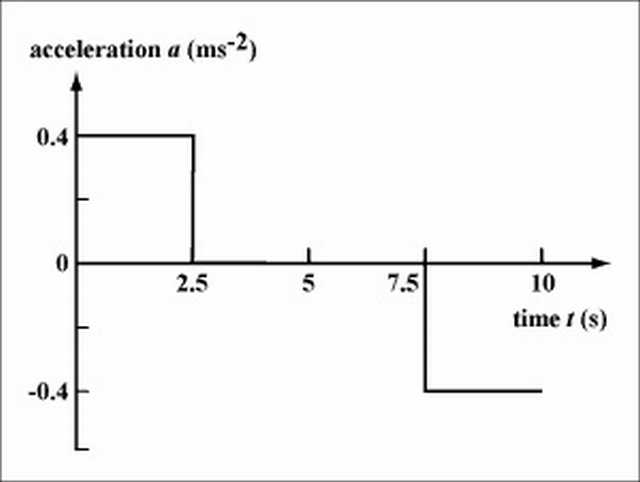
\includegraphics[scale=0.5]{Images/CC/P-Graphs/4.1e/Images/Kinematics/5-11}%
\end{minipage}}
\begin{description}
\item [{Question}] : Acceleration vs time graphs for five objects are shown
below. All axis have the same scale. Which object has the greatest
change in velocity during the interval?
\end{description}
\doublebox{\begin{minipage}[t]{0.72\columnwidth}%
\includegraphics[scale=0.5]{Images/CC/P-Graphs/Common/Reduced/reviewkinematics/ImagesReduced/TUGK2\lyxdot jpg}%
\end{minipage}}

\cite{www.physport.org}

\section{One More Go in a different perspective}

\subsection{Distance-Time Graphs}

\doublebox{\begin{minipage}[t]{0.72\columnwidth}%
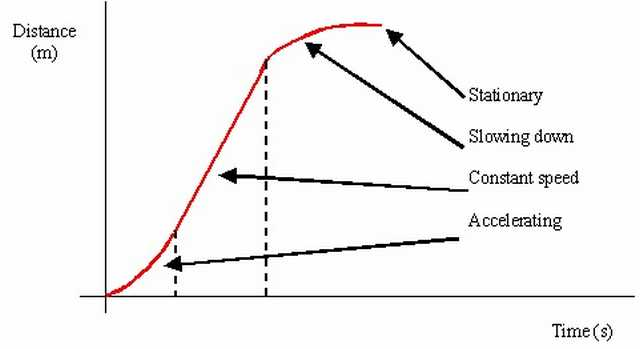
\includegraphics[scale=0.5]{Images/CC/P-Graphs/4.1e/Images/Kinematics/distance-time-graph1}%
\end{minipage}}

For a distance-time graph, the distance never decreases. When the
object is stationary, the distance-time graph will be horizontal.
The gradient of a distance-time graph is the instantaneous speed of
the object. For straight line with positive gradient, it means that
the object is travelling at uniform speed There is no straight line
with negative gradient (as the distance never decreases) For curves,
it means that the object is travelling at non-uniform speed \cite{www.miniphysics.com}

\subsection{Displacement-time graphs}

The details are similar as distance-time graphs, except that the distance
is now displacement, and speed is now velocity. One minor difference:
There is a straight line with negative gradient, it means that the
object is travelling at uniform velocity in the opposite direction.\cite{www.miniphysics.com}

\subsection{Velocity-time graphs}

\doublebox{\begin{minipage}[t]{0.72\columnwidth}%
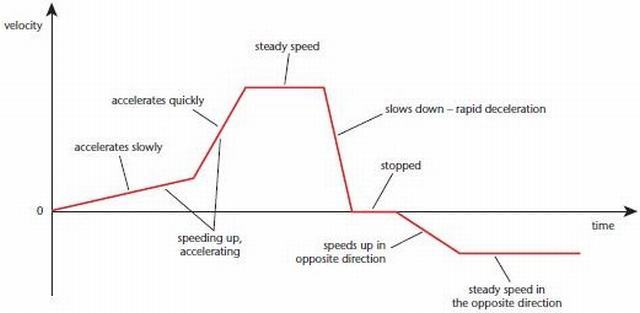
\includegraphics[scale=0.5]{Images/CC/P-Graphs/4.1e/Images/Kinematics/velocity-time-graph}%
\end{minipage}}

When the object is stationary, it is a straight horizontal line at
0. When the object is undergoing uniform motion, it is a straight
horizontal line at vm s\textminus 1vm s\textminus 1, where v is the
velocity of the object. For straight line with positive gradient,
it means that the object is accelerating. For straight line with negative
gradient, it means that the object is decelerating. For curves, it
means that the acceleration of the object is changing. The area under
the graph is the change in displacement of the object 

\subsection{Acceleration-time graphs}

Area under graph is the change in velocity \cite{www.miniphysics.com}

The figure below shows the displacement-time graph, velocity-time
graph and acceleration-time graph for the respective state of motion.
It serves as a summary of the text above.

\doublebox{\begin{minipage}[t]{0.72\columnwidth}%
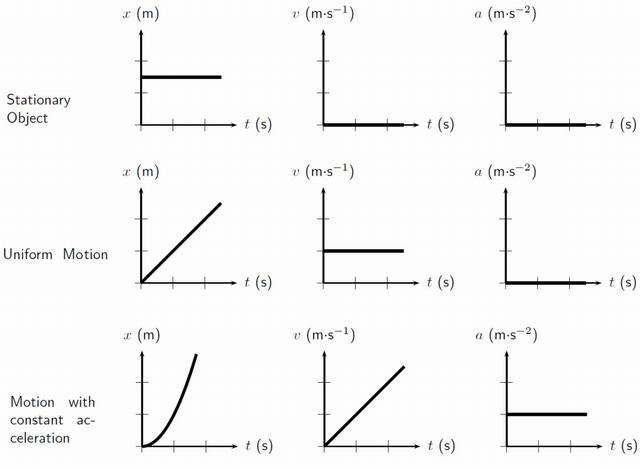
\includegraphics[scale=0.5]{Images/CC/P-Graphs/4.1e/Images/Kinematics/all-graphs-of-motion-1024x751}%
\end{minipage}}\cite{www.sparknotes.com}

\subsection{Self-Test Questions\cite{www.miniphysics.com}}

Q Can you tell from a displacement-time graph whether an object is
stationary?

Answer Yes. If the object is stationary, it will appear as a horizontal
line on a displacement-time graph.

Q How can you obtain the average velocity and instantaneous velocity
from a displacement-time graph.

Answer The average velocity can be found by using$\dfrac{total\;displacement}{total\;time\;taken}$

The instantaneous velocity at a point in time can be found from the
gradient of the tangent to that point in time.

Q Can you tell from a velocity-time graph whether an object is stationary?

Answer Yes. If the object is stationary, the velocity-time graph will
be a horizontal line at v=0.

QHow would you obtain the acceleration of an object from a velocity-time
graph? What does the area under a velocity-time graph represent?

Answer The acceleration of an object at a point in time can be obtained
from the gradient of the tangent to that point in time.

The area under a velocity-time graph represents the total distance
traveled.

Q Can you tell from an acceleration-time graph whether an object is
stationary?

Answer No, you cannot. Do you know why?

\section{Revision}

Since you are not allowed to use calculators, SAT II Physics places
a heavy emphasis on qualitative problems. A common way of testing
kinematics qualitatively is to present you with a graph plotting position
vs. time, velocity vs. time, or acceleration vs. time and to ask you
questions about the motion of the object represented by the graph.
Because SAT II Physics is entirely made up of multiple-choice questions,
you won\textquoteright t need to know how to draw graphs; you\textquoteright ll
just have to interpret the data presented in them. Knowing how to
read such graphs quickly and accurately will not only help you solve
problems of this sort, it will also help you visualize the often-abstract
realm of kinematic equations. In the examples that follow, we will
examine the movement of an ant running back and forth along a line.\cite{www.sparknotes.com}

\doublebox{\begin{minipage}[t]{0.72\columnwidth}%
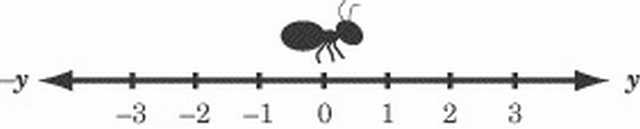
\includegraphics[scale=0.5]{Images/CC/P-Graphs/4.1e/Images/Kinematics/ant}%
\end{minipage}}

\subsection{Position vs. Time Graphs}

Position vs. time graphs give you an easy and obvious way of determining
an object\textquoteright s displacement at any given time, and a subtler
way of determining that object\textquoteright s velocity at any given
time. Let\textquoteright s put these concepts into practice by looking
at the following graph charting the movements of our friendly ant.\cite{www.sparknotes.com}

\doublebox{\begin{minipage}[t]{0.72\columnwidth}%
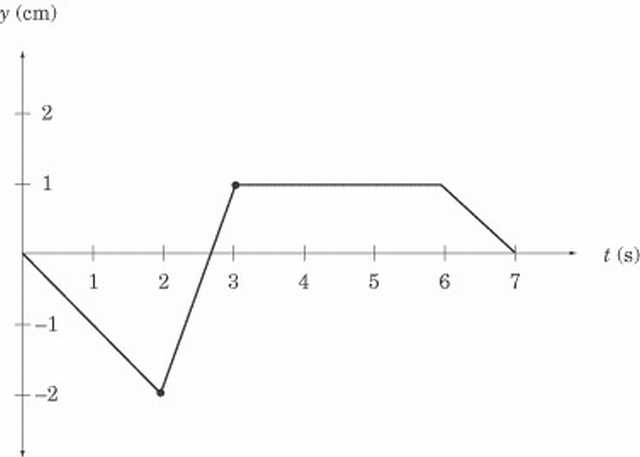
\includegraphics[scale=0.5]{Images/CC/P-Graphs/4.1e/Images/Kinematics/YvsTgraph}%
\end{minipage}}

Any point on this graph gives us the position of the ant at a particular
moment in time. For instance, the point at (2,\textendash 2) tells
us that, two seconds after it started moving, the ant was two centimeters
to the left of its starting position, and the point at (3,1) tells
us that, three seconds after it started moving, the ant is one centimeter
to the right of its starting position. Let\textquoteright s read what
the graph can tell us about the ant\textquoteright s movements. For
the first two seconds, the ant is moving to the left. Then, in the
next second, it reverses its direction and moves quickly to y = 1.
The ant then stays still at y = 1 for three seconds before it turns
left again and moves back to where it started. Note how concisely
the graph displays all this information. Calculating Velocity We know
the ant\textquoteright s displacement, and we know how long it takes
to move from place to place. Armed with this information, we should
also be able to determine the ant\textquoteright s velocity, since
velocity measures the rate of change of displacement over time. If
displacement is given here by the vector y, then the velocity of the
ant is

$v=\dfrac{\triangle y}{\triangle t}$

If you recall, the slope of a graph is a measure of rise over run;
that is, the amount of change in the y direction divided by the amount
of change in the x direction. In our graph, is the change in the y
direction and is the change in the x direction, so v is a measure
of the slope of the graph. For any position vs. time graph, the velocity
at time t is equal to the slope of the line at t. In a graph made
up of straight lines, like the one above, we can easily calculate
the slope at each point on the graph, and hence know the instantaneous
velocity at any given time. We can tell that the ant has a velocity
of zero from t = 3 to t = 6, because the slope of the line at these
points is zero. We can also tell that the ant is cruising along at
the fastest speed between t = 2 and t = 3, because the position vs.
time graph is steepest between these points. Calculating the ant\textquoteright s
average velocity during this time interval is a simple matter of dividing
rise by run, as we\textquoteright ve learned in math class.

\subsection{Average Velocity }

$velocity=\dfrac{y_{final}-y_{initial}}{t_{final}-t_{initial}}$

$=\dfrac{1-(-2)\,cm}{3-2s}$

=3 cm/s to the right

How about the average velocity between t = 0 and t = 3? It\textquoteright s
actually easier to sort this out with a graph in front of us, because
it\textquoteright s easy to see the displacement at t = 0 and t =
3, and so that we don\textquoteright t confuse displacement and distance.

\subsection{Average Speed }

Although the total displacement in the first three seconds is one
centimeter to the right, the total distance traveled is two centimeters
to the left, and then three centimeters to the right, for a grand
total of five centimeters. Thus, the average speed is not the same
as the average velocity of the ant. Once we\textquoteright ve calculated
the total distance traveled by the ant, though, calculating its average
speed is not difficult:

5cm/3s = 1.67cm/s

\subsection{Curved Position vs. Time Graphs }

This is all well and good, but how do you calculate the velocity of
a curved position vs. time graph? Well, the bad news is that you\textquoteright d
need calculus. The good news is that SAT II Physics doesn\textquoteright t
expect you to use calculus, so if you are given a curved position
vs. time graph, you will only be asked qualitative questions and won\textquoteright t
be expected to make any calculations. A few points on the graph will
probably be labeled, and you will have to identify which point has
the greatest or least velocity. Remember, the point with the greatest
slope has the greatest velocity, and the point with the least slope
has the least velocity. The turning points of the graph, the tops
of the \textquotedblleft hills\textquotedblright{} and the bottoms
of the \textquotedblleft valleys\textquotedblright{} where the slope
is zero, have zero velocity.\cite{www.sparknotes.com}

\doublebox{\begin{minipage}[t]{0.72\columnwidth}%
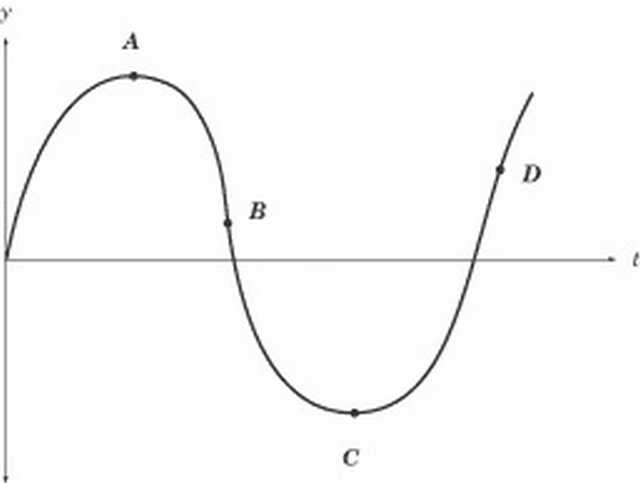
\includegraphics[scale=0.5]{Images/CC/P-Graphs/4.1e/Images/Kinematics/curvedYvsTgraph}%
\end{minipage}}

In this graph, for example, the velocity is zero at points A and C,
greatest at point D, and smallest at point B. The velocity at point
B is smallest because the slope at that point is negative. Because
velocity is a vector quantity, the velocity at B would be a large
negative number. However, the speed at B is greater even than the
speed at D: speed is a scalar quantity, and so it is always positive.
The slope at B is even steeper than at D, so the speed is greatest
at B. Velocity vs. Time Graphs Velocity vs. time graphs are the most
eloquent kind of graph we\textquoteright ll be looking at here. They
tell us very directly what the velocity of an object is at any given
time, and they provide subtle means for determining both the position
and acceleration of the same object over time. The \textquotedblleft object\textquotedblright{}
whose velocity is graphed below is our ever-industrious ant, a little
later in the day.

\doublebox{\begin{minipage}[t]{0.72\columnwidth}%
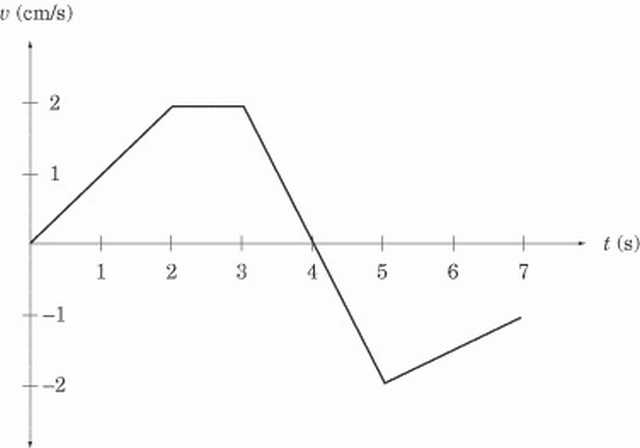
\includegraphics[scale=0.5]{Images/CC/P-Graphs/4.1e/Images/Kinematics/VvsTgraph}%
\end{minipage}}

We can learn two things about the ant\textquoteright s velocity by
a quick glance at the graph. First, we can tell exactly how fast it
is going at any given time. For instance, we can see that, two seconds
after it started to move, the ant is moving at 2 cm/s. Second, we
can tell in which direction the ant is moving. From t = 0 to t = 4,
the velocity is positive, meaning that the ant is moving to the right.
From t = 4 to t = 7, the velocity is negative, meaning that the ant
is moving to the left. Calculating Acceleration We can calculate acceleration
on a velocity vs. time graph in the same way that we calculate velocity
on a position vs. time graph. Acceleration is the rate of change of
the velocity vector, , which expresses itself as the slope of the
velocity vs. time graph. For a velocity vs. time graph, the acceleration
at time t is equal to the slope of the line at t. What is the acceleration
of our ant at t = 2.5 and t = 4? Looking quickly at the graph, we
see that the slope of the line at t = 2.5 is zero and hence the acceleration
is likewise zero. The slope of the graph between t = 3 and t = 5 is
constant, so we can calculate the acceleration at t = 4 by calculating
the average acceleration between t = 3 and t = 5:

$velocity=\dfrac{y_{final}-y_{initial}}{t_{final}-t_{initial}}$

=$\dfrac{-2-(2)\,cm/s}{5-3\;s}$

= -2 cm/s$^{2}$

The minus sign tells us that acceleration is in the leftward direction,
since we\textquoteright ve defined the y-coordinates in such a way
that right is positive and left is negative. At t = 3, the ant is
moving to the right at 2 cm/s, so a leftward acceleration means that
the ant begins to slow down. Looking at the graph, we can see that
the ant comes to a stop at t = 4, and then begins accelerating to
the right. \cite{www.sparknotes.com}

\subsection{Calculating Displacement }

Velocity vs. time graphs can also tell us about an object\textquoteright s
displacement. Because velocity is a measure of displacement over time,
we can infer that:

displacement = velocity $\times$ time

Graphically, this means that the displacement in a given time interval
is equal to the area under the graph during that same time interval.
If the graph is above the t-axis, then the positive displacement is
the area between the graph and the t-axis. If the graph is below the
t-axis, then the displacement is negative, and is the area between
the graph and the t-axis. Let\textquoteright s look at two examples
to make this rule clearer. First, what is the ant\textquoteright s
displacement between t = 2 and t = 3? Because the velocity is constant
during this time interval, the area between the graph and the t-axis
is a rectangle of width 1 and height 2.

\doublebox{\begin{minipage}[t]{0.72\columnwidth}%
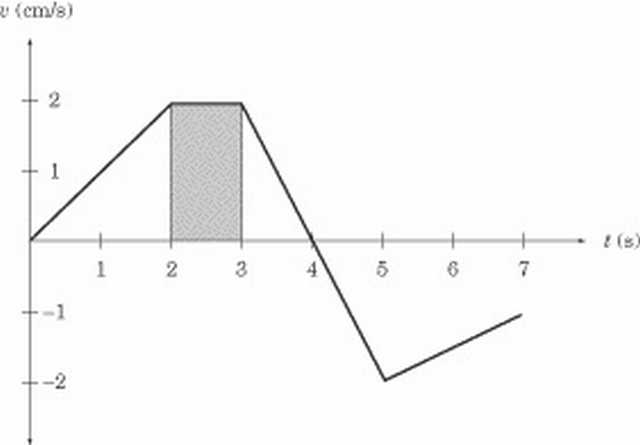
\includegraphics[scale=0.5]{Images/CC/P-Graphs/4.1e/Images/Kinematics/VvsTgraph_shade1}%
\end{minipage}}

The displacement between t = 2 and t = 3 is the area of this rectangle,
which is 2 cm/s.1s = 2 cm to the right. Next, consider the ant\textquoteright s
displacement between t = 3 and t = 5. This portion of the graph gives
us two triangles, one above the t-axis and one below the t-axis.

\doublebox{\begin{minipage}[t]{0.72\columnwidth}%
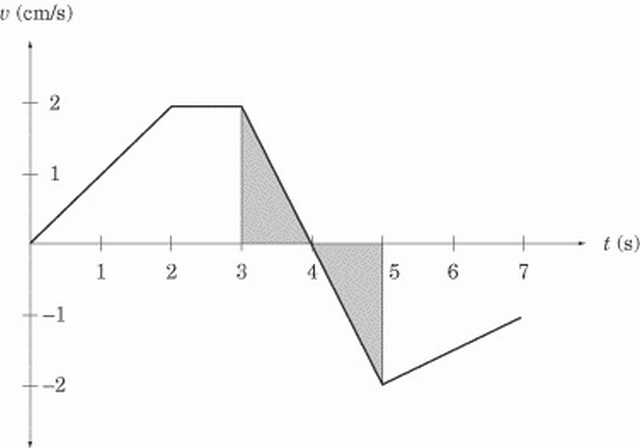
\includegraphics[scale=0.5]{Images/CC/P-Graphs/4.1e/Images/Kinematics/VvsTgraph_shade2}%
\end{minipage}}

Both triangles have an area of 1 /2(1 s)(2 cm/s) = 1 cm. However,
the first triangle is above the t-axis, meaning that displacement
is positive, and hence to the right, while the second triangle is
below the t-axis, meaning that displacement is negative, and hence
to the left. The total displacement between t = 3 and t = 5 is \textbf{ZERO}.

In other words, at t = 5, the ant is in the same place as it was at
t = 3. \cite{www.sparknotes.com}

\subsection{Curved Velocity vs. Time Graphs }

As with position vs. time graphs, velocity vs. time graphs may also
be curved. Remember that regions with a steep slope indicate rapid
acceleration or deceleration, regions with a gentle slope indicate
small acceleration or deceleration, and the turning points have zero
acceleration. 

\subsection{Acceleration vs. Time Graphs}

After looking at position vs. time graphs and velocity vs. time graphs,
acceleration vs. time graphs should not be threatening. Let\textquoteright s
look at the acceleration of our ant at another point in its dizzy
day.

\doublebox{\begin{minipage}[t]{0.72\columnwidth}%
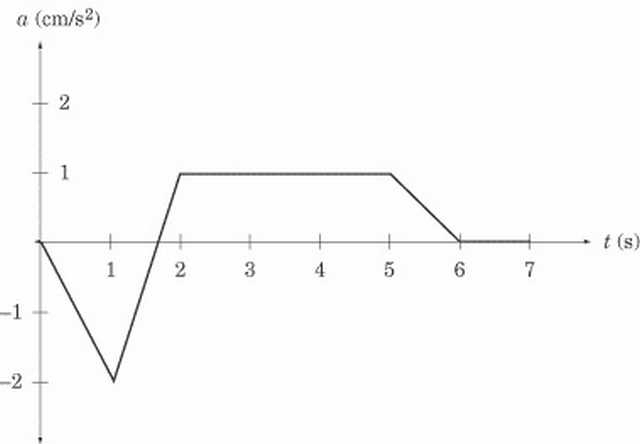
\includegraphics[scale=0.5]{Images/CC/P-Graphs/4.1e/Images/Kinematics/AvsTgraph}%
\end{minipage}}

Acceleration vs. time graphs give us information about acceleration
and about velocity. SAT II Physics generally sticks to problems that
involve a constant acceleration. In this graph, the ant is accelerating
at 1 m/s2 from t = 2 to t = 5 and is not accelerating between t =
6 and t = 7; that is, between t = 6 and t = 7 the ant\textquoteright s
velocity is constant.\cite{www.sparknotes.com}

\subsection{Calculating Change in Velocity}

Acceleration vs. time graphs tell us about an object\textquoteright s
velocity in the same way that velocity vs. time graphs tell us about
an object\textquoteright s displacement. The change in velocity in
a given time interval is equal to the area under the graph during
that same time interval. Be careful: the area between the graph and
the t-axis gives the change in velocity, not the final velocity or
average velocity over a given time period. What is the ant\textquoteright s
change in velocity between t = 2 and t = 5? Because the acceleration
is constant during this time interval, the area between the graph
and the t-axis is a rectangle of height 1 and length 3.\cite{www.sparknotes.com}

\doublebox{\begin{minipage}[t]{0.72\columnwidth}%
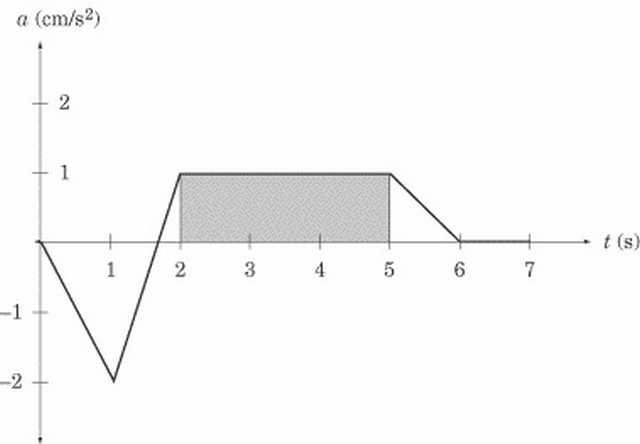
\includegraphics[scale=0.5]{Images/CC/P-Graphs/4.1e/Images/Kinematics/AvsTgraph_shade1}%
\end{minipage}}

The area of the shaded region, and consequently the change in velocity
during this time interval, is 1 cm/s2 � 3 s = 3 cm/s to the right.
This doesn\textquoteright t mean that the velocity at t = 5 is 3 cm/s;
it simply means that the velocity is 3 cm/s greater than it was at
t = 2. Since we have not been given the velocity at t = 2, we can\textquoteright t
immediately say what the velocity is at t = 5. Summary of Rules for
Reading Graphs You may have trouble recalling when to look for the
slope and when to look for the area under the graph. Here are a couple
handy rules of thumb: The slope on a given graph is equivalent to
the quantity we get by dividing the y-axis by the x-axis. For instance,
the y-axis of a position vs. time graph gives us displacement, and
the x-axis gives us time. Displacement divided by time gives us velocity,
which is what the slope of a position vs. time graph represents. The
area under a given graph is equivalent to the quantity we get by multiplying
the x-axis and the y-axis. For instance, the y-axis of an acceleration
vs. time graph gives us acceleration, and the x-axis gives us time.
Acceleration multiplied by time gives us the change in velocity, which
is what the area between the graph and the x-axis represents. We can
summarize what we know about graphs in a table: 

\doublebox{\begin{minipage}[t]{0.72\columnwidth}%
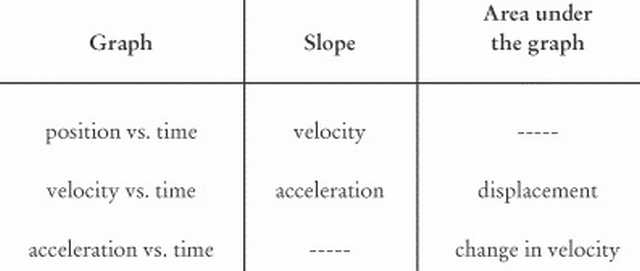
\includegraphics[scale=0.5]{Images/CC/P-Graphs/4.1e/Images/Kinematics/graphsummary}%
\end{minipage}}

\section{Exercises}

\subsection{Problems on Position-Time Graph}

\subsubsection{Subjectives}

\strong{Example} : A boy walks at a velocity of 0.5 m/s along a street
for 50 s, suddenly he remembers that he has to buy something in a
shop that he has passed by, so he turns around and walks at a velocity
of -1 m/s for 10 s. He then stops for 30 s at the shop, and finally
walks forward again at 0.5 m/s for another 20 s. Plot a displacement-time
graph for the motion of the boy.\cite{www.hk-phy.org}

\strong{Solution} : See Fig. 5-4.

\doublebox{\begin{minipage}[t]{0.72\columnwidth}%
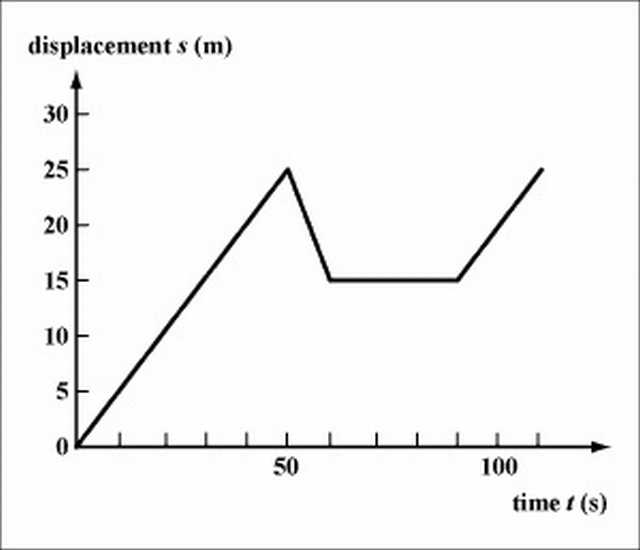
\includegraphics[scale=0.5]{Images/CC/P-Graphs/4.1e/Images/Kinematics/5-04}%
\end{minipage}}

\strong{Example} : A marathon runner runs at a constant 12 km/h.\cite{intmath.com}

a. Express her displacement travelled as a function of time.

b. Graph the motion for ${\displaystyle 0\le t\le4h}$

\strong{Solution} : a. ${\displaystyle s=12t}$, for displacement
s and time t.

b. Graph of ${\displaystyle s=12t.}$

\doublebox{\begin{minipage}[t]{0.72\columnwidth}%
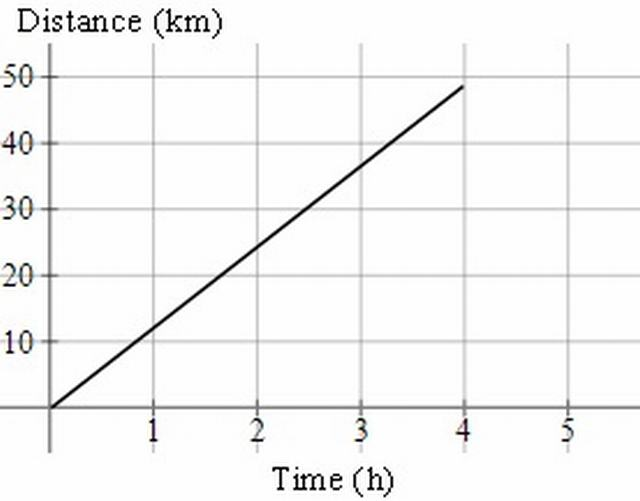
\includegraphics[scale=0.5]{Images/CC/P-Graphs/4.1e/Images/Kinematics/kinematics4-g}%
\end{minipage}}

We stop the graph at (4, 48).

\strong{Example} : This is the graph of a journey by sports car:\cite{intmath.com}

\doublebox{\begin{minipage}[t]{0.72\columnwidth}%
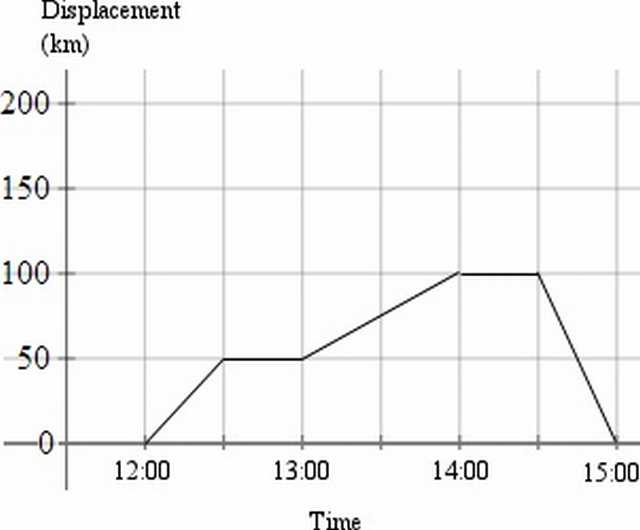
\includegraphics[scale=0.5]{Images/CC/P-Graphs/4.1e/Images/Kinematics/kinematics2-g}%
\end{minipage}}

a. What is the velocity for each stage of the journey?

b. What is the average (mean) velocity for the whole journey?

\strong{Solution} : a. This table outlines the stages of the journey.

\begin{tabular}{|c|c|}
\hline 
12:00 to 12:30 & Travelled 50 km in30 minutes, so 100 km/h\tabularnewline
\hline 
\hline 
12:30 to 13:00 & Stopped\tabularnewline
\hline 
13:00 to 14:00 & Travelled 50 km in 60 minutes, so 50 km/h\tabularnewline
\hline 
14:00 to 14:30 & Stopped\tabularnewline
\hline 
14:30 to 15:00 & Travelled 100 km back towards the starting point in 30 minutes, so
\textminus 200 km/h\tabularnewline
\hline 
\end{tabular}

b. Even though the whole journey was 200 km (100 km out and 100 km
back) in 3 hours, the displacement for the journey (the distance from
the starting point) is 0km.

So the average velocity is 0 km/h.

On the other hand, the average speed was ${\displaystyle \frac{200}{3}=66.7\ \text{km/h}}$

In summary,

${\displaystyle \text{ave velocity}=\frac{\text{displacement}}{\text{time}}}$

${\displaystyle \text{ave speed}=\frac{\text{distance}}{\text{time}}}$

\strong{Example }: A particle in a magnetic field moves as follows:\cite{intmath.com}

\doublebox{\begin{minipage}[t]{0.72\columnwidth}%
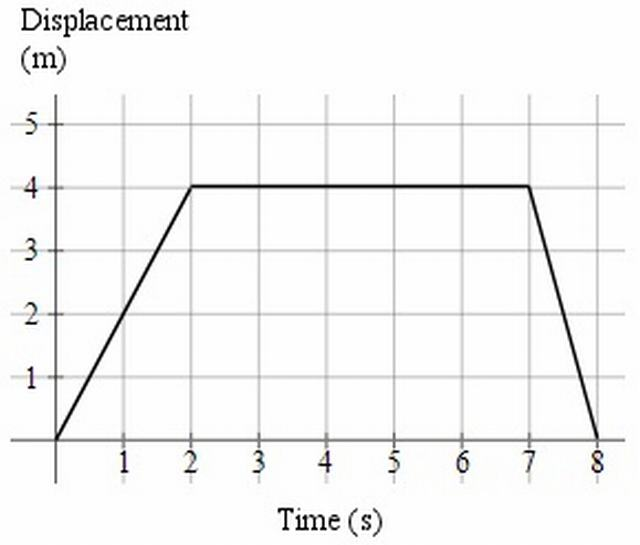
\includegraphics[scale=0.5]{Images/CC/P-Graphs/4.1e/Images/Kinematics/kinematics3-g}%
\end{minipage}}

Find the velocity for each part of the motion.

\strong{Solution} :

For t=0 to 2: ${\displaystyle \frac{\Delta s}{\Delta t}=\frac{4}{2}=2\ \text{ms}^{-1}}$ 

For t=2 to 7: ${\displaystyle \frac{\Delta s}{\Delta t}=\frac{0}{5}=0\ \text{ms}^{-1}}$

For t=7 to 8:${\displaystyle \frac{\Delta s}{\Delta t}=\frac{-4}{2}=-4\ \text{ms}^{-1}}$ 

(The velocity is negative, since the particle is going in the opposite
direction.)

\strong{Example} : An object's position during a 10 second time interval
is shown by the graph below:

\doublebox{\begin{minipage}[t]{0.72\columnwidth}%
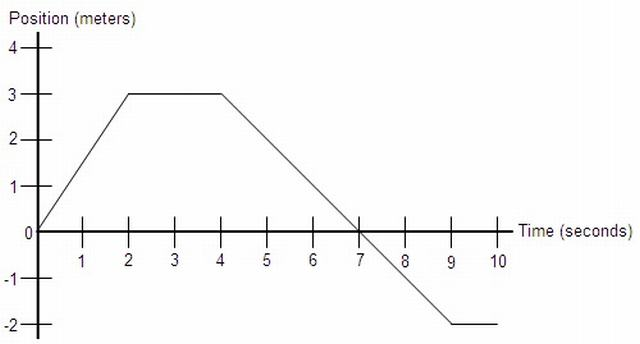
\includegraphics[scale=0.5]{Images/CC/P-Graphs/4.1e/Images/Kinematics/ex22}%
\end{minipage}}

a.) Determine the object's total distance traveled and displacement.

b.) What is the object's velocity at the following times: t = 1, t
= 3, and t = 6. 

c.) Determine the object's average velocity and average speed from
t = 0 to t = 10.

d.) What is the object's acceleration at t = 5?

\strong{Solution} : a.) The total distance traveled by the object
is the sum of all the distances it traveled during the time interval.
In the first two seconds it traveled 3 m. Then it traveled 0 m in
the next two seconds. Then over the next five seconds, the object
moved 5 m, then remained at rest. so the total distance is 3 + 5 =
8 m. The displacement of the object is simply the final position minus
the initial position, or -2 - 0 = -2 m.

b.) Notice that each of these points is in the middle of a line segment
on the graph. Because of this, the instantaneous velocity at these
points is the same as the average velocity over the time intervals
represented by each segment, so: v(t) = (xf - xi)/(tf - ti) v(1) =
(3 - 0)/(2 - 0) = 3/2 = 1.5 m/s v(3) = (3 - 3)/(4 - 2) = 0/2 = 0 m/s
v(6) = (-2 - 3)/(9 - 4) = -5/5 = -1 m/s

Notice that the formula (xf - xi)/(tf - ti) is the same as the slope
formula for this graph. The velocity at any point on a position vs.
time graph is simply the slope of the graph at that point. By this
definition, we also know that the velocity of any position function
is its derivative with respect to time. You can also go from a velocity
function to a position function using integration. Go to calculus
notes

c.) Average velocity is displacement divided by time. We found in
part a that the object's displacement is -2 m, so: vavg = -2/10 =
-0.2 m/s

Average speed is total distance divided be time, and we found in part
a that the object's total distance traveled is 8 m. so: 8/10 = 0.8
m/s

d.) We determined in part b that the object's velocity is represented
by the slope of the line segment on the graph. Since the slope of
this segment is constant, the object's velocity at t = 5 is constant.
Since constant velocity means there is no acceleration, a = 0.

\subsection{Problems on Velocity-Time Graph}

\subsubsection{Subjective}

\strong{Example} : Fig. shows the velocity-time graph of a train
travelling from station 1 to station 2. The train moves along a straight
railway.

\doublebox{\begin{minipage}[t]{0.72\columnwidth}%
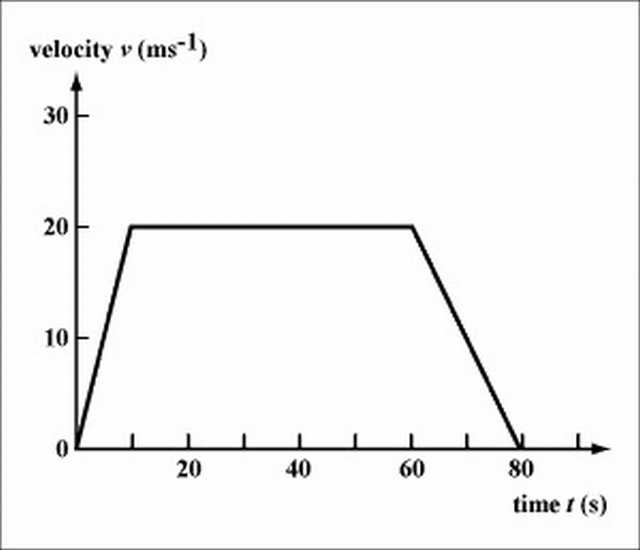
\includegraphics[scale=0.5]{Images/CC/P-Graphs/4.1e/Images/Kinematics/5-07}%
\end{minipage}}

Describe the motion of the train, stating the acceleration and velocity
in each stage. What is the displacement of station 2 from station
1? 

\strong{Solution} : From t=0 to t=10s , the train accelerates from
v=0 to v=20m/s .

a=20/10=2 m s$^{-2}$

From t=10s to t=60s , the train moves at a constant velocity v=20m/s.
a=0 .

From t=60s to t=80s , the train decelerates from v=20m/s back to v=0m/s
.

a=(0-20)/(80-60)=-1m s$^{-2}$

Total displacement = the area under the velocity-time graph

$s=\dfrac{(80+50)}{2}\times20=1300m$

\strong{Example} : A car is initially moving at a velocity of 36
. Suddenly the driver sees a girl running across of the road at 13
m in front of the car. It takes 0.5 s for the driver to react and
start braking the car. The car then takes one more second to stop.
Plot the velocity-time graph for the car, starting from the time when
the driver sees the girl. What is the deceleration of the car? Would
the car hit the girl?

\doublebox{\begin{minipage}[t]{0.72\columnwidth}%
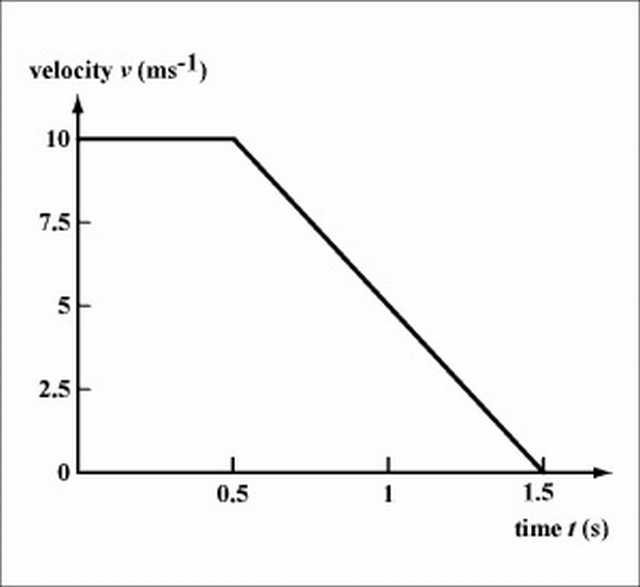
\includegraphics[scale=0.5]{Images/CC/P-Graphs/4.1e/Images/Kinematics/5-08}%
\end{minipage}}

Solution : See Fig. . The car decelerates at 10 ms$^{-2}$. It travels
a total distance of (0.5+1.5){*}10/2=10m , so it would not hit the
girl, but stop at a distance of 3 m from the girl.

Note: The total distance travelled by the car after the driver seeing
the danger is called the stopping distance. See the next chapter for
more analysis on car braking.

\strong{Example} ; Fig. shows the displacement-time graph of an object.
Plot its velocity-time graph. Find the average velocity of the object.

\doublebox{\begin{minipage}[t]{0.72\columnwidth}%
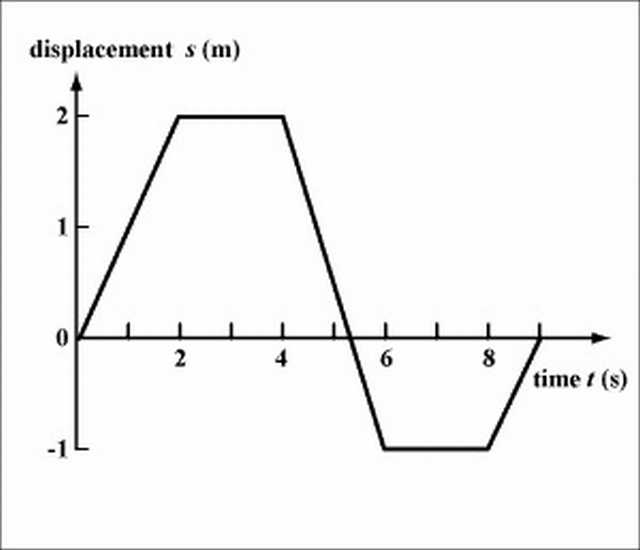
\includegraphics[scale=0.5]{Images/CC/P-Graphs/4.1e/Images/Kinematics/5-09}%
\end{minipage}}

\strong{Solution} : See Fig. .

\doublebox{\begin{minipage}[t]{0.72\columnwidth}%
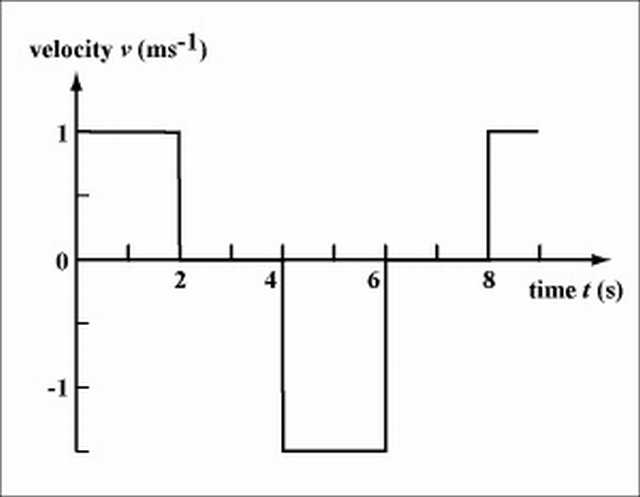
\includegraphics[scale=0.5]{Images/CC/P-Graphs/4.1e/Images/Kinematics/5-10}%
\end{minipage}}

Since the total displacement of the object is zero, the average velocity
is also zero.

Note: The object moves backwards from t=4s to t=6s . In this interval,
the area bounded by the velocity-time graph is negative (i.e., the
area is under the time axis), indicating that the object has a displacement
in the opposite direction.

\strong{Example} : A particle in a generator is accelerated from
rest at the rate of 55 ms $^{-2}$ .

a. What is the velocity at t=3 s?

b. What is the acceleration at t=3 s?

c. What is the distance travelled in 3 seconds?

d. Graph the acceleration (as a v - t graph) for ${\displaystyle 0\le t\le3\ \text{s}0\le t\le3s}$.

\strong{Solution} : a. Velocity =55\texttimes 3=165 ms $^{-1}$ 

b. The acceleration is a constant 55 ms $^{-2}$ , so at t=3 s, the
acceleration will be 55 ms$^{-2}$ .

c. The distance travelled in \textbackslash displaystyle 3 seconds
is 165\texttimes 1.5=247.5 m. We obtain this from the area under the
line between 0 and 3 (i.e. the area of the shaded triangle below).

d. Note in the graph that we have velocity on the vertical axis, and
the units are m/s.

The graph finishes at (3, 165).

\doublebox{\begin{minipage}[t]{0.72\columnwidth}%
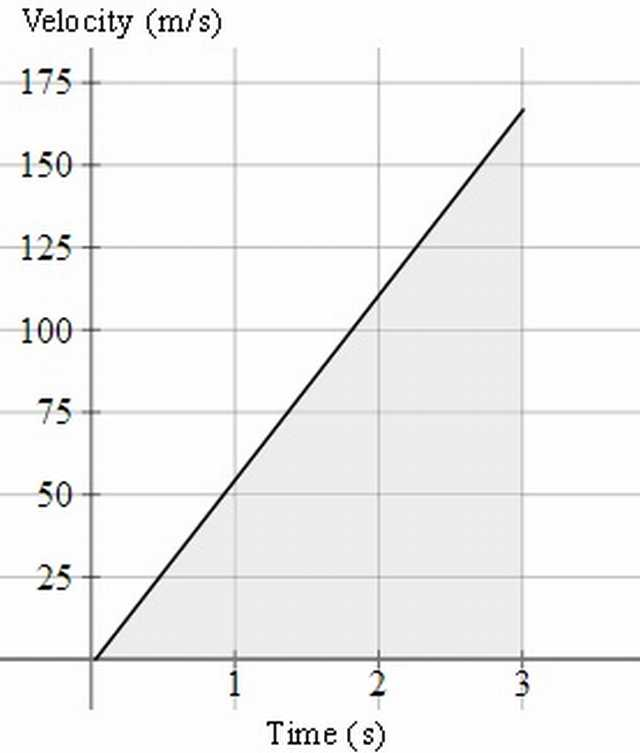
\includegraphics[scale=0.5]{Images/CC/P-Graphs/4.1e/Images/Kinematics/kinematics6-g}%
\end{minipage}}

\strong{Example} : A girl starts from rest and travels along a straight
line. The diagram below shows the velocity-time graph of the girl
from 0 s to 90 s.

\doublebox{\begin{minipage}[t]{0.72\columnwidth}%
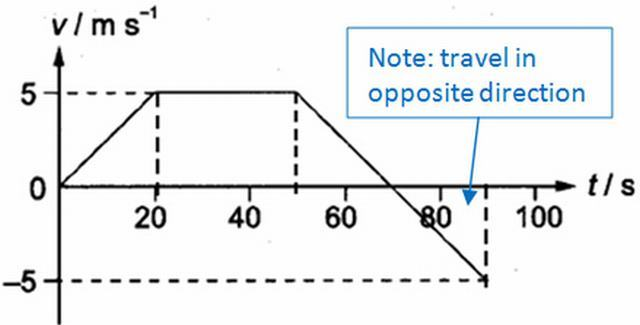
\includegraphics[scale=0.5]{Images/CC/P-Graphs/4.1e/Images/Kinematics/8312034}%
\end{minipage}}

(a) Describe the motion of the girl from 0 s to 40 s.

(b) Find the average velocity of the girl in the first 70 s. 

(c) Draw the acceleration-time graph of the girl from 0 s to 90 s.

(d) Find the displacement of the girl from the starting point to the
position at 90 s. 

\strong{Solution} : (a) From 0 s to 20 s, she travels with constant
acceleration of 0.25 ms\textasciicircum (-2); From 20 s to 40 s,
she travels at constant velocity of 5 m/s. 

(b) Total displacement = area under v-t graph = \textonehalf{} (30
+ 70) {*} 5 = 250 m Average velocity = 250/70 = 3.57 m/s 

(c) Acceleration is the gradient of v-t graph. 

\doublebox{\begin{minipage}[t]{0.72\columnwidth}%
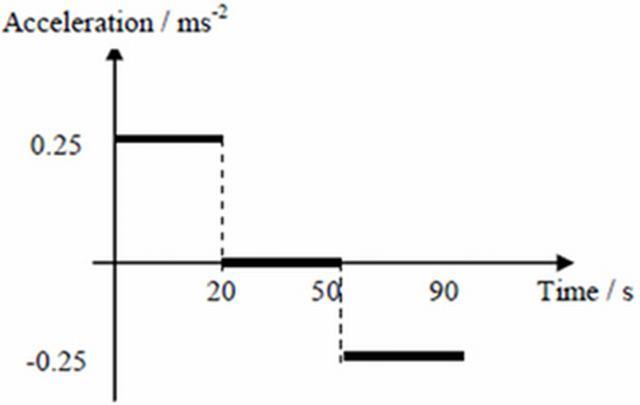
\includegraphics[scale=0.5]{Images/CC/P-Graphs/4.1e/Images/Kinematics/7365655}%
\end{minipage}}

(d) Displacement = area under v-t graph = 250 \textendash{} \textonehalf{}
{*} 20 {*} 5 = 200 m

Tips: (1) It is very easy to mix up kinematics graphs. The only way
to differentiate these graphs is to look at the y-axis!

(2) When describing the motion, do it region by region! And always
talk about acceleration or speed / velocity with values if applicable.
Refer to example above.

\strong{Example} : Two sport cars start from rest at the same place.
One of them, colored red, accelerates at 0.90 ms $^{-2}$ for 15 s,
and continues at constant speed thereafter. The other car, colored
blue, accelerates at 0.85ms $^{-2}$ for 20 s and then remains at
that speed.

Draw both journeys on the same velocity-time graph and determine the
time and distance that the second car overtakes the first car.

\strong{Solution} :

\doublebox{\begin{minipage}[t]{0.72\columnwidth}%
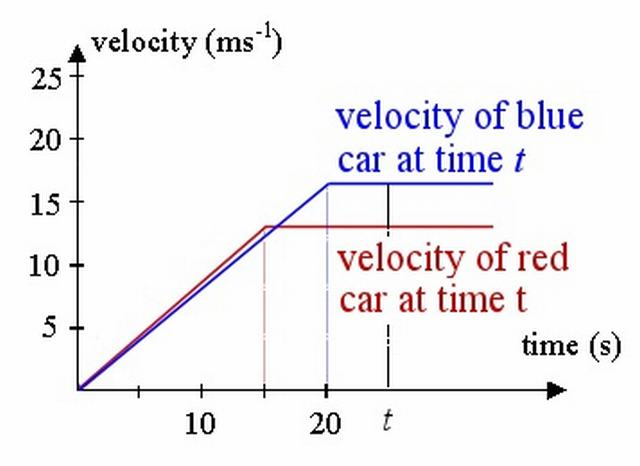
\includegraphics[scale=0.5]{Images/CC/P-Graphs/4.1e/Images/Kinematics/ex4a}%
\end{minipage}}

The velocities they reach are 0.9 \texttimes{} 15 = 13.5 ms-1 and
0.85 \texttimes{} 20 = 17 ms-1 respectively.

Similar to the problem above, we have:

First car's (red) distance at time t is found by finding the area
of the trapezoid whose boundary is the t-axis, the red lines and the
vertical line representing time at t seconds. This of course assumes
t\textgreater 15 (otherwise, we have negative distances, and the
trapezoid only starts at t=15.)

So the distance (at time t)${\displaystyle =\frac{1}{2}\times13.5\left(t+t-15\right)}$

= The distance of the second car (blue) is found by finding the area
of the blue trapezoid, bounded by the blue lines, the t-axis and the
vertical line. (And this one assumes t\textgreater 20, for the same
reasons as above.)

So the distance (at time t)${\displaystyle =\frac{1}{2}\times17\left(t+t-20\right)}$

The distance when they meet is the same, so:

${\displaystyle \frac{1}{2}\times13.5\times\left(2t-15\right)}$=$\frac{1}{2}\times17\times\left(2t-20\right)$ 

Solving gives:

Time =19.643 s 

Distance=163.93 m

Dilemma

However, this solution gives us a dilemma. As mentioned above, the
expressions we found for the area of the trapezoids required t to
be more than 15 s and 20 s, respectively.

We can confirm the blue car overtakes the red car before 20 seconds,
by calculating the distances travelled at that time.

After 20 seconds:

Red car has travelled 0.5\texttimes (20+5)\texttimes 13.5=168.75 m

Blue car has travelled 0.5\texttimes 20\texttimes 17=170 m The blue
car has travelled further than the red car, so it means it has already
overtaken the red car.

Back to the drawing board

So, in fact, for this question we need to consider the area of the
blue triangle, not the blue trapezoid.

This is the correct diagram for finding t:

\doublebox{\begin{minipage}[t]{0.72\columnwidth}%
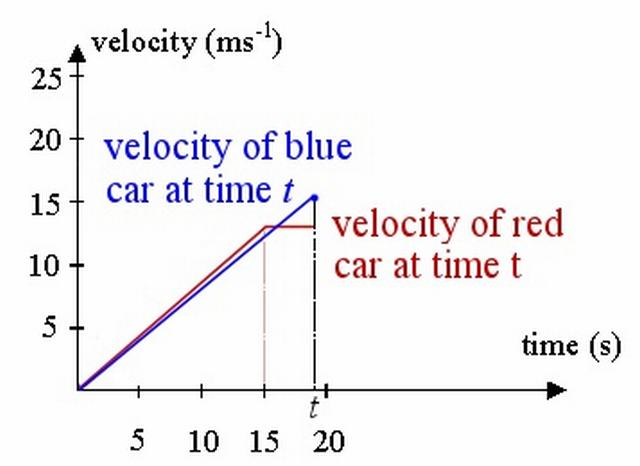
\includegraphics[scale=0.5]{Images/CC/P-Graphs/4.1e/Images/Kinematics/ex4a2}%
\end{minipage}}

The red car's distance is fine from before (it's a trapezoid):

${\displaystyle d=\frac{1}{2}\times13.5\left(t+t-15\right)}$

But the blue car's distance at t is the area of the triangle (not
trapezoid) bounded by the blue line and the vertical line at t (we
are taking ${\displaystyle \frac{1}{2}}$ base times height):

$distance{\displaystyle =\frac{1}{2}\times t\times0.85\times t}$

Equating these gives:

6.75(2t \textminus{} 15) = 0.425t$^{2}$

Solving gives:

t =12.14 s, t = 19.63 s

The first solution has no practical meaning, since t\textgreater 15
for the expression to work.

So we conclude the time taken for the blue car to overtake the red
car is 19.63 s and the distance travelled at that time is 163.7 m.

Further Information

To illustrate we have found the correct answer, below is the graph
of distance against time. Labelling of axes is very important in this
work!

The red curve corresponds to the acceleration portion of the first
race car. At t=15, or point C(15,101.25), the red car stops accelerating
and continues at a constant speed (CA is no longer a curve, but a
straight line).

The blue curve corresponds to the second (blue) car. It doesn't accelerate
as hard (its curve is below the red curve, indicating it covers less
distance in the same time), but it accelerates for longer. At t=20,
or point D (20,170), it stops accelerating and its graph is now a
straight line.

We can see the curves intersect at time t=19.63 s, or point A (19.63,163.7),
as we found in the calculation above. This means they have covered
the same distance (163.7 m) at that time, so that's when the blue
car passes the red car.

\doublebox{\begin{minipage}[t]{0.72\columnwidth}%
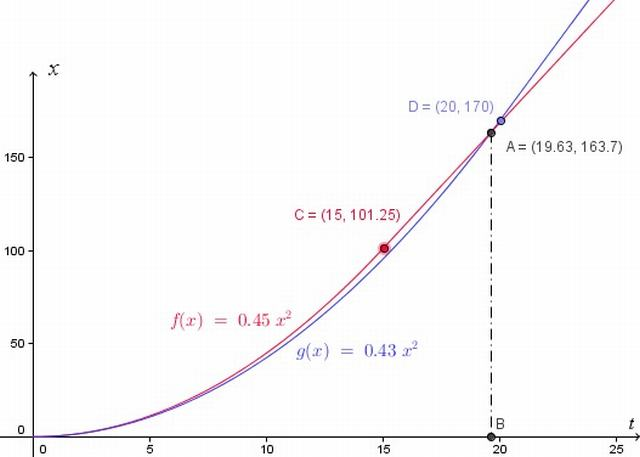
\includegraphics[scale=0.5]{Images/CC/P-Graphs/4.1e/Images/Kinematics/race-cars2}%
\end{minipage}}

\subsubsection{Miscelleneous}

\strong{Example} : You drive a car in such a way that its motion
is described by the velocity-time graph shown here. Draw the displacement-time
and acceleration-time graphs that correspond to this motion, and describe
in words how the car moves.\cite{www.uwgb.edu}

\doublebox{\begin{minipage}[t]{0.72\columnwidth}%
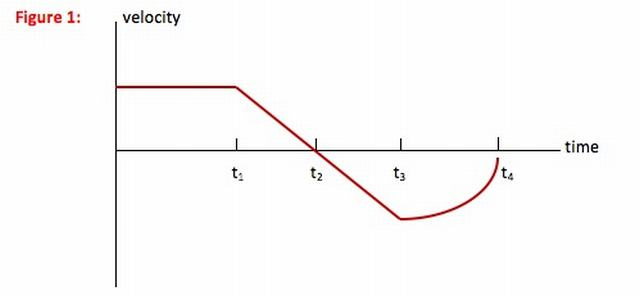
\includegraphics[scale=0.5]{Images/CC/P-Graphs/4.1e/Images/Kinematics/fig1}%
\end{minipage}}

\strong{Solution} : (Hint : In this problem, you are asked to describe
the motion of the car. Whenever you are asked to describe the motion
of an object without worrying about the cause of that motion, you
have a kinematics problem. This problem is different from most kinematics
problems, however, in that you are not asked for a numerical description
but rather to use words and graphs to describe how the car moves.)

(Queries : How did you know that x = 0 at t = 0? 

You don\textquoteright t! If you are given a velocity-time graph,
you know the initial speed but not the initial location of the object.
(Calculus students, remember v = dx/dt, and the derivative of a constant\textemdash your
initial location\textemdash is zero.) I chose to call the location
of the car at t = 0 the origin, but you could start your graph at
any point. The shape of the graph, however, should look the same. 

Why can\textquoteright t I treat the straight line from t1 to t3 in
a single step? 

Any time velocity is above the t-axis, it has a positive value and
so slope of the x-t graph is also positive. A positive slope means
that the line or curve is in such a direction as to make between a
0 and a 900 angle above the +x axis. Any time velocity is below the
t-axis, it has a negative value and so the slope of the x-t graph
is also negative. A negative slope means that the line or curve is
in such a direction as to make between a 0 and a 900 angle below the
+x axis.

Why doesn\textquoteright t the line from t3 to t4 look more curved? 

As the velocity-time curve gets closer and closer to v = 0 (the t-axis),
velocity\textquoteright s value is getting smaller regardless of direction.
As the value of v decreases, so does the slope of the x-t graph. A
decreasing slope means that the slope gets smaller and smaller\textemdash the
line gets becomes more horizontal.

The curve from t3 to t4 on the x-t graph shown here doesn\textquoteright t
look very curved. This is because its slope goes from the same value
as it ended with on the t2 to t3 curve to almost zero (a horizontal
line) and so not a lot of change as I have drawn it. Any line you
draw that curves down and to the right becoming more horizontal as
it goes is fine.)

Select a relation

To go between a velocity-time graph and a displacement-time or acceleration-time
graph, you need to understand how velocity, displacement and acceleration
are related to each other. In other words, you need to use the definitions
of velocity and acceleration:

v = \textgreek{D}x/\textgreek{D}t In words, the value of velocity
= the slope of the x-t graph.

a = \textgreek{D}v/\textgreek{D}t In words, the value of acceleration
= the slope of the v-t graph.

Hint: Graphing problems seem like they should be straightforward,
and the equations that you need are only those given above. It is
very, very common, however, to make mistakes on these problems because
it feels like the graphs should be pictures of the motion and they
are not. In order to avoid those mistakes, make a table based on the
sentences above and then draw the graph from the table. 

Displacement-Time Graph

\doublebox{\begin{minipage}[t]{0.72\columnwidth}%
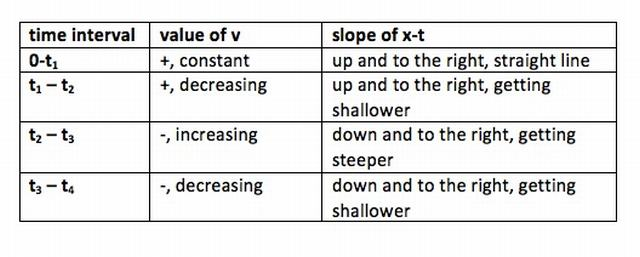
\includegraphics[scale=0.5]{Images/CC/P-Graphs/4.1e/Images/Kinematics/solve}%
\end{minipage}}

\doublebox{\begin{minipage}[t]{0.72\columnwidth}%
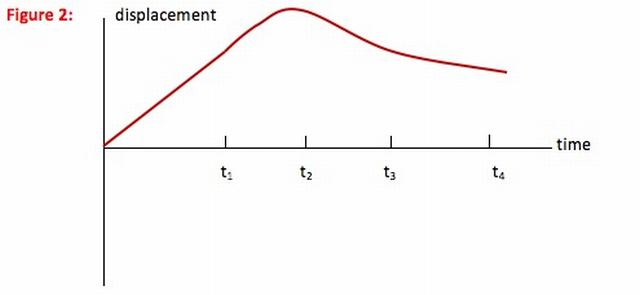
\includegraphics[scale=0.5]{Images/CC/P-Graphs/4.1e/Images/Kinematics/fig2}%
\end{minipage}}

Once you understand the displacement-time graph, continue down to
the acceleration-time graph.

Acceleration-time Graph

\doublebox{\begin{minipage}[t]{0.72\columnwidth}%
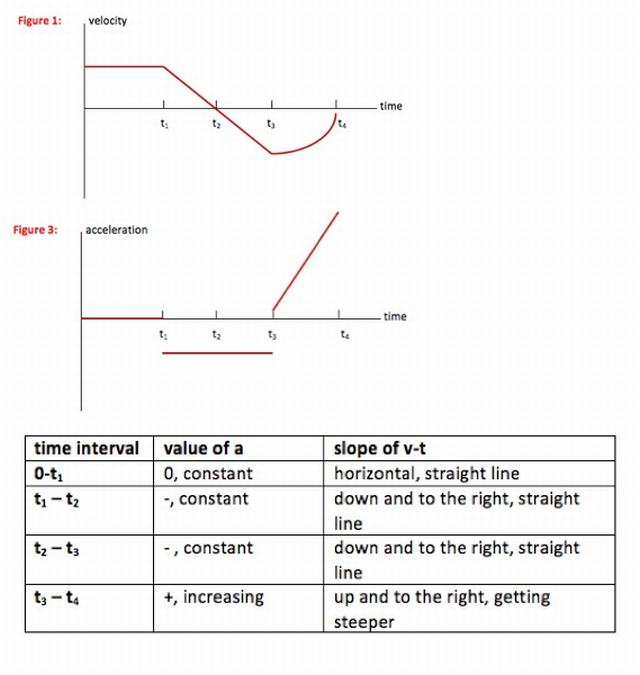
\includegraphics[scale=0.5]{Images/CC/P-Graphs/4.1e/Images/Kinematics/solve1}%
\end{minipage}}

Understand

In this problem, you are given the velocity-time graph for the motion
of a car. By relating the value of velocity to the slope of the x-t
graph (this is just the definition of velocity) you are able to draw
the x-t graph corresponding to this motion.

By relating the slope of the v-t graph to the value of acceleration
(this is just the definition of acceleration) you are able to draw
the a-t graph corresponding to this motion.

You can describe the motion looking at any of the three graphs. From
t = 0 to t1 : The car travels forward (+ direction) with a constant
speed. There is no acceleration and the car moves away from its starting
point at a constant rate.

From t1 to t2 : The car slows to a stop at a constant rate. It is
still moving forward, but the amount of distance it covers in each
second is decreasing. Acceleration acts against the motion of the
car, or in the negative direction.

From t2 to t3 : The car reverses direction, moving faster and faster
(at a constant acceleration) in the negative direction. Acceleration
is acting with the motion of the car, so it is also in the negative
direction. The amount of distance the car covers each second increases.

From t3 to t4 : The car continues to move in the negative direction
but at a decreasing speed. The rate at which the speed decreases is
getting greater\textemdash the driver is braking harder as the car
stops\textemdash and so acceleration increases. Acceleration is acting
against the motion of the car, or in the positive direction. The car
covers less and less distance each second.

\subsection{Problems on Area Under v-t graph}

\strong{Example} : A charged particle in an accelerator starts from
rest, accelerates at 1.5 ms $^{-2}$ for3 s and then continues at
a steady speed for a further 6 s.

Draw the v-t graph and find the total distance travelled.

\strong{Solution}:

\doublebox{\begin{minipage}[t]{0.72\columnwidth}%
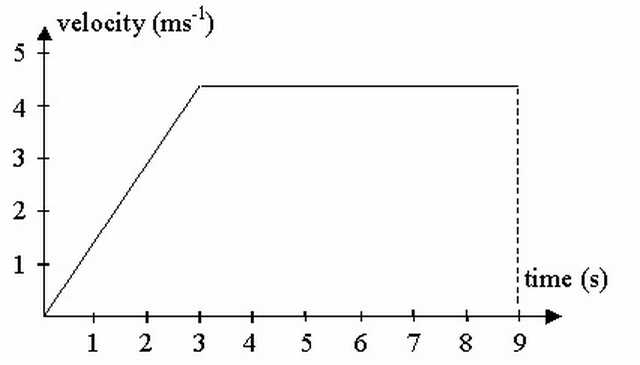
\includegraphics[scale=0.5]{Images/CC/P-Graphs/4.1e/Images/Kinematics/ex}%
\end{minipage}}

Total distance travelled is the area under the graph (in this case
we need to find the area of a trapezium).

${\displaystyle \text{distance}=\frac{\left(a+b\right)h}{2}}$

${\displaystyle =\frac{\left(9+6\right)\times4.5}{2}}$

=33.75 m

\strong{Example} : A car is travelling at a constant speed of 72
km/h and passes a stationary police car. The police car immediately
gives chase, accelerating uniformly to reach a speed of 90 km/h in
10 s and continues at this speed until he overtakes the other car.
Find:

(a) the time taken by the police to catch up with the car,

(b) the distance travelled by the police car when this happens.

\strong{Solution} :

\doublebox{\begin{minipage}[t]{0.72\columnwidth}%
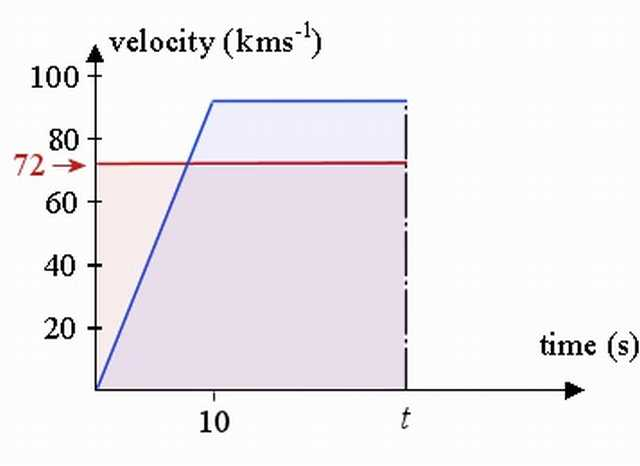
\includegraphics[scale=0.5]{Images/CC/P-Graphs/4.1e/Images/Kinematics/ex3a}%
\end{minipage}}

The v-t curve for the car is represented by the red line, while that
v-t curve for the police car is the blue line.

We need to find the unknown time t (in seconds), when the police catch
up to the car. We find this by comparing the distance travelled by
each (it will be the same distance at the overtaking point.) So we
need to set the area under the v-t curve for the car (the pink shaded
area) to be equal to the area under the v-t curve for the police car
(the blue shaded area).

a. The area under the curve for the car at time t (in seconds) is
simply 72t. (It is a rectangle, 72 high and width t).

The area under the trapezium (trapezoid) for the police car at unknown
time t, using ${\displaystyle A=\left(a+b\right)\frac{h}{2}}$ is:

${\displaystyle \left(t+t-10\right)\times\frac{90}{2}}$=$45\left(2t-10\right)$

We set these equal to find the required time: 72t=45(2t\textminus 10)
That is, when 72t=90t\textminus 450 So t=25 s will be the time the
police car catches up.

b. Both of the cars have travelled $72\times\left(\frac{25}{3600}\right)\times1000=500\ \text{m}$
during those 25 s.

{[}We have used d=s\texttimes t and converted from seconds to hours
(since the velocities are given in km/h).{]}

\subsection{Problems on Average Velocity}

\strong{Example} : An object's velocity during a 10 second time interval
is shown by the graph below:

\doublebox{\begin{minipage}[t]{0.72\columnwidth}%
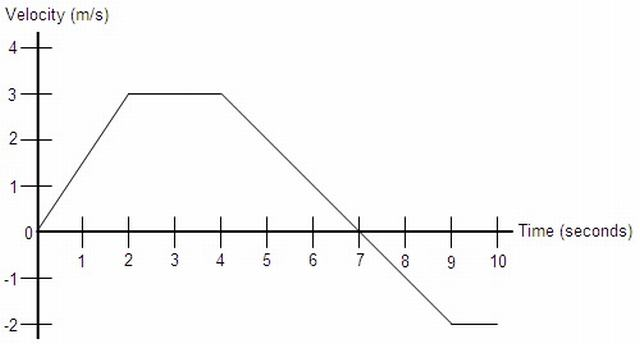
\includegraphics[scale=0.5]{Images/CC/P-Graphs/4.1e/Images/Kinematics/ex23}%
\end{minipage}}

a.) Determine the object's total distance traveled and displacement.

b.) At t = 0, the object's position is x = 2 m. Find the object's
position at t = 2, t = 4, t = 7, and t = 10. 

c.) What is the object's acceleration at the following times: t =
1, t = 3, and t = 6. 

d.) Sketch the corresponding acceleration vs. time graph from t =
0 to t = 10.

\strong{Solution} : a.) Recall that the equation for velocity is
v = x/t. If we solve this for x, we get x = vt. Notice that this is
the same as the area of a rectangles whose sides are lengths v and
t, so we can determine that the displacement is the area enclosed
by the velocity vs. time graph. So, we will find the area of each
section under the graph:

\doublebox{\begin{minipage}[t]{0.72\columnwidth}%
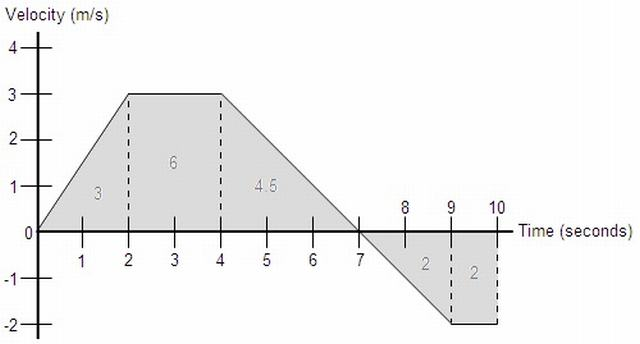
\includegraphics[scale=0.5]{Images/CC/P-Graphs/4.1e/Images/Kinematics/ex23a}%
\end{minipage}}

The total distance traveled by the object is simply the sum of all
these areas: 3 + 6 + 4.5 + 2 + 2 = 17.5 m The displacement is found
in a similar fashion, except areas below the x-axis are considered
negative: 3 + 6 + 4.5 - 2 - 2 = 9.5 m Interestingly enough, the area
enclosed by any function can be represented by a definite integral.
For example, if this graph were defined as a function v(t), then the
displacement would be the integral from 0 to 10 of v(t)dt, and the
total distance traveled would be the integral from 0 to 10 of \textbar v(t)\textbar dt
Go to calculus notes

b.) The position of the object at a given point in time can be found
in much the same way we found the displacement in part a, except this
time we must also add in the initial value given. So: x(2) = 2 + 3
= 5 m x(4) = 2 + 3 + 6 = 11 m x(7) = 2 + 3 + 6 + 4.5 = 15.5 m x(10)
= 2 + 3 + 6 + 4.5 - 2 - 2 = 11.5 m

Notice that this can also be done by adding the integral from 0 to
t of v(t)dt to the initial value of 2. Go to calculus notes

c.) Like velocity in part b of problem 22, the instantaneous acceleration
at any point along one of the graph's line segments is the same as
the average acceleration across that line segment. The formula for
acceleration is aavg = \textgreek{D}v/\textgreek{D}t = (vf - vi)/(tf
- ti), so: a(t) = (vf - vi)/(tf - ti) a(1) = (3 - 0)/(2 - 0) = 3/2
= 1.5 m/s2 a(3) = (3 - 3)/(4 - 2) = 0/2 = 0 m/s2 a(6) = (-2 - 3)/(9
- 4) = -5/5 = -1 m/s2

Similarly to the relationship between velocity and position, the formula
for acceleration is the same as the slope formula for a velocity vs.
time graph. So, we can say that the slope of any velocity vs. time
graph is its acceleration. Notice that this definition defines acceleration
as the derivative of velocity. So, it is true that for any velocity
function v(t), its derivative is an acceleration function a(t). Also,
integration can be used to go from an acceleration function to a position
function. Go to calculus notes

d.) We know that the acceleration along each line segment of this
velocity vs. time graph is equal to the slope of the line segment.
We determined these slopes in part c, so the acceleration graph would
look like:

\doublebox{\begin{minipage}[t]{0.72\columnwidth}%
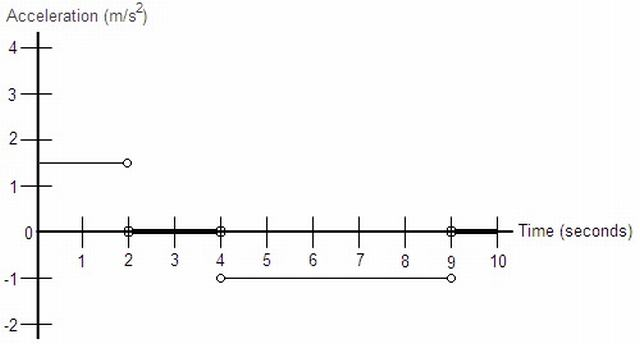
\includegraphics[scale=0.5]{Images/CC/P-Graphs/4.1e/Images/Kinematics/ex23d}%
\end{minipage}}

This graph uses horizontal lines instead of points to represent that
the acceleration is defined at that value at any point along that
section. The open circles at the end of each line segment simply indicate
that at those time values, acceleration is not defined at either value
represented by the horizontal lines. At these points, acceleration
is undefined because it changes instantaneously from one value to
the next, which cannot be represented numerically.

\chapter{Few Basic Problems}

\paragraph{Problem Set 1}

Use the following graph to answer Questions \#1 - \#7.

\doublebox{\begin{minipage}[t]{0.9\columnwidth}%
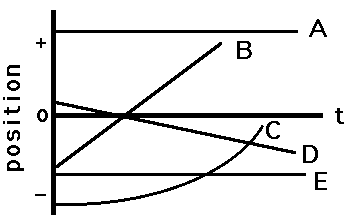
\includegraphics{Images/CC/P-Graphs/4.1e/Images/Kinematics/graph01}%
\end{minipage}}

1. Which object(s) is(are) maintaining a state of motion (i.e., maintaining
a constant velocity)? 

Answer ; Objects A, B, D, and E. 

Objects A, B, D, and E are maintaining a state of motion (i.e., remaining
with constant velocity) as demonstrated by the constant slope. If
the slope is constant, then the velocity is constant.

2. Which object(s) is(are) accelerating? 

Answer : Object C

Object C is accelerating. An accelerating object has a changing velocity.
Since the slope of a p-t graph equals the velocity, an accelerating
object is represented by a changing slope.

3. Which object(s) is(are) not moving? 

Answer : Objects A and E.

Objects A and E are not moving. An object which is not moving has
a zero velocity; this translates into a line with zero slope on a
p-t graph. 

4. Which object(s) change(s) its direction? 

Answer : None of the objects change direction.

None of these objects change direction. An object changes its direction
if it changes from a + to a - velocity (or vice versa). This translates
into a p-t graph with a + slope and then a - slope (or vice versa).

5. On average, which object is traveling fastest? 

Answer : Object B.

Object B is traveling fastest. To be traveling fastest is to have
the greatest speed (or greatest magnitude of velocity). This translates
into the line on a p-t graph with the greatest slope. 

6. On average, which moving object is traveling slowest? 

Answer : Object D.

Object D is traveling slowest. To be traveling slowest is to have
the smallest speed (or smallest magnitude of velocity). This translates
into the line on a p-t graph with the smallest slope.

7. Which object has the greatest acceleration? 

Answer ; Object C.

Object C has the greatest acceleration. It is the only object with
an acceleration. Accelerated motion on a p-t graph is represented
by a curved line.

\paragraph{Problem Set 2}

Use the following graph to answer Questions \#8 - \#13.

\doublebox{\begin{minipage}[t]{0.9\columnwidth}%
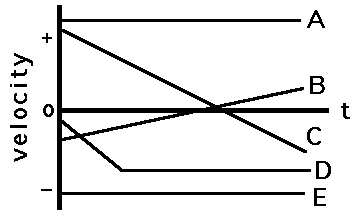
\includegraphics{Images/CC/P-Graphs/4.1e/Images/Kinematics/graph08}%
\end{minipage}}

8. Which object(s) is(are) maintaining its state of motion? 

Answer : Objects A and E.

Objects A and E are maintaining their state of motion. To maintain
the state of motion is to keep a constant velocity (i.e., to have
a zero acceleration). This translates into a zero slope on a v-t graph.

9. Which object(s) is(are) accelerating? 

Answer : Objects B and C (and D during the first part of its motion).

Objects B and C are accelerating (and for a while, object D). Accelerated
motion is indicated by a sloped line on a v-t graph. 

10. Which object(s) is(are) not moving? 

Answer : Each of the objects are moving.

Each of the objects are moving. If an object were not moving, then
the v-t graph would be a horizontal line along the axis (v = 0 m/s). 

11. Which object(s) change(s) its direction? 

Answer : Objects B and C.

Objects B and C change their direction. An object that is changing
its direction is changing from a + to a - velocity. Thus, the line
on a v-t graph will pass from the + to the - region of the graph.
Object D is not changing its direction; object D first moves in the
- direction with increasing speed and then maintains a constant speed.

12. Which accelerating object has the smallest acceleration? 

Answer : Object B.

Object B has the smallest acceleration. Acceleration is indicated
by the slope of the line. The object with the smallest acceleration
is the object with the smallest slope.

13. Which object has the greatest velocity? 

Answer : Object A (E is a close second place).

Object A has the greatest velocity (and object E is a \textquotedbl close
second\textquotedbl ). The velocity is indicated by how far above
or how far below the axis the line is. Object A has a large + velocity.
Object E has a large (but not as large) - velocity.

\paragraph{Problem Set 3}

14. Sketch a position-time graph for an object which is moving with
a constant, positive velocity. 

Answer : A position-time graph for an object which is moving with
a constant, positive velocity is shown below. A positive, constant
velocity is represented by a line with constant slope (straight) and
positive slope (upwards sloping).

\doublebox{\begin{minipage}[t]{0.9\columnwidth}%
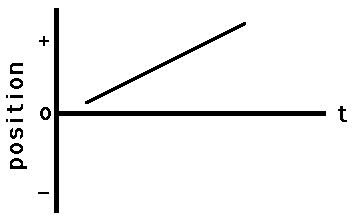
\includegraphics{Images/CC/P-Graphs/4.1e/Images/Kinematics/graph14}

Graph of Question 14%
\end{minipage}}

15. Sketch a position-time graph for an object which is moving with
a constant, negative velocity. 

Answer : A position-time graph for an object which is moving with
a constant, negative velocity is shown below. A negative, constant
velocity is represented by a line with constant slope (straight) and
negative slope (downwards sloping).

\doublebox{\begin{minipage}[t]{0.9\columnwidth}%
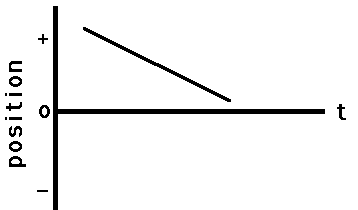
\includegraphics{Images/CC/P-Graphs/4.1e/Images/Kinematics/graph15}

Graph of Question 15%
\end{minipage}}

16. Sketch a position-time graph for an object moving in the + dir'n
and accelerating from a low velocity to a high velocity. 

Answer : A position-time graph for an object moving in the + dir'n
and accelerating from a low velocity to a high velocity is shown below.
If the object is moving in the + dir'n, then the slope of a p-t graph
would be +. If the object is changing velocity from small to large
values, then the slope must change from small slope to large slope.

\doublebox{\begin{minipage}[t]{0.9\columnwidth}%
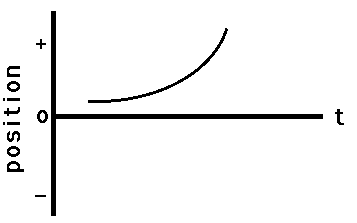
\includegraphics{Images/CC/P-Graphs/4.1e/Images/Kinematics/graph16}

Graph of Question 16%
\end{minipage}}

17. Sketch a position-time graph for an object moving in the + dir'n
and accelerating from a high velocity to a low velocity. 

Answer : A position-time graph for an object moving in the + dir'n
and accelerating from a high velocity to a low velocity is shown below.
If the object is moving in the + dir'n, then the slope of a p-t graph
would be +. If the object is changing velocity from high to low values,
then the slope must change from high slope to low slope.

\doublebox{\begin{minipage}[t]{0.9\columnwidth}%
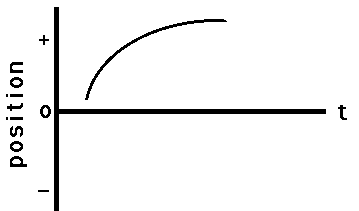
\includegraphics{Images/CC/P-Graphs/4.1e/Images/Kinematics/graph17}

Graph of Question 17%
\end{minipage}}

18. Sketch a position-time graph for an object moving in the - dir'n
and accelerating from a high velocity to a low velocity. 

Answer : A position-time graph for an object moving in the - dir'n
and accelerating from a high velocity to a low velocity is shown below.
If the object is moving in the - dir'n, then the slope of a p-t graph
would be -. If the object is changing velocity from high to low values,
then the slope must change from high slope to low slope.

\doublebox{\begin{minipage}[t]{0.9\columnwidth}%
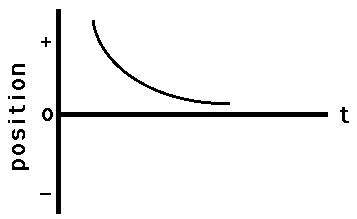
\includegraphics{Images/CC/P-Graphs/4.1e/Images/Kinematics/graph18}

Graph of Question 18%
\end{minipage}}

19. Sketch a position-time graph for an object moving in the - dir'n
and accelerating from a low velocity to a high velocity. 

Answer : A position-time graph for an object moving in the - dir'n
and accelerating from a low velocity to a high velocity is shown below.
If the object is moving in the - dir'n, then the slope of a p-t graph
would be -. If the object is changing velocity from low to high values,
then the slope must change from low slope to high slope.

\doublebox{\begin{minipage}[t]{0.9\columnwidth}%
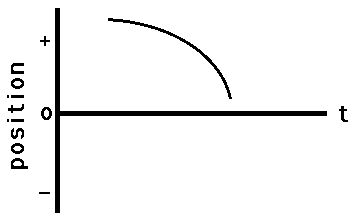
\includegraphics{Images/CC/P-Graphs/4.1e/Images/Kinematics/graph19}

Graph of Question 19%
\end{minipage}}

20. Sketch a position-time graph for an object moving in the + dir'n
with constant speed; first a slow constant speed and then a fast constant
speed. 

Answer : A position-time graph for an object moving in the + dir'n
with constant speed; first a slow constant speed and then a fast constant
speed is shown below. If an object is moving in the + dir'n, then
the slope of the line on a p-t graph would be +. At first, the line
has a small slope (corresponding to a small velocity) and then the
line has a large slope (corresponding to a large velocity).

\doublebox{\begin{minipage}[t]{0.9\columnwidth}%
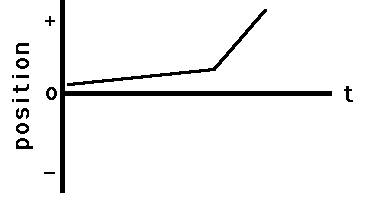
\includegraphics{Images/CC/P-Graphs/4.1e/Images/Kinematics/graph20}

Graph of Question 20%
\end{minipage}}

21. Sketch a position-time graph for an object moving in the + dir'n
with constant speed; first a fast constant speed and then a slow constant
speed. 

Answer : A position-time graph for an object moving in the + dir'n
with constant speed; first a fast constant speed and then a slow constant
speed is shown below. If an object is moving in the + dir'n, then
the slope of the line on a p-t graph would be +. At first, the line
has a large slope (corresponding to a large velocity) and then the
line has a small slope (corresponding to a small velocity).

\doublebox{\begin{minipage}[t]{0.9\columnwidth}%
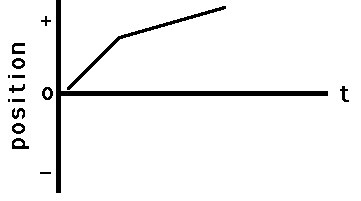
\includegraphics{Images/CC/P-Graphs/4.1e/Images/Kinematics/graph21}

Graph of Question 21%
\end{minipage}}

22. Sketch a position-time graph for an object moving in the - dir'n
with constant speed; first a slow constant speed and then a fast constant
speed. 

Answer : A position-time graph for an object moving in the - dir'n
with constant speed; first a slow constant speed and then a fast constant
speed is shown below. If an object is moving in the - dir'n, then
the slope of the line on a p-t graph would be -. At first, the line
has a small slope (corresponding to a small velocity) and then the
line has a large slope (corresponding to a large velocity).

\doublebox{\begin{minipage}[t]{0.9\columnwidth}%
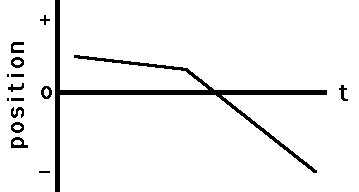
\includegraphics{Images/CC/P-Graphs/4.1e/Images/Kinematics/graph22}

Graph of Question 22%
\end{minipage}}

23. Sketch a position-time graph for an object moving in the - dir'n
with constant speed; first a fast constant speed and then a slow constant
speed. 

Answer : A position-time graph for an object moving in the - dir'n
with constant speed; first a fast constant speed and then a slow constant
speed is shown below. If an object is moving in the - dir'n, then
the slope of the line on a p-t graph would be -. At first, the line
has a large slope (corresponding to a large velocity) and then the
line has a small slope (corresponding to a small velocity).

\doublebox{\begin{minipage}[t]{0.9\columnwidth}%
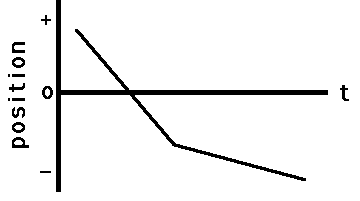
\includegraphics{Images/CC/P-Graphs/4.1e/Images/Kinematics/graph23}

Graph of Question 23%
\end{minipage}}

24. Sketch a position-time graph for an object which moves in the
+ direction at a slow constant speed and then in a - direction at
a fast constant speed. 

Answer : A position-time graph for an object which moves in the +
direction at a slow constant speed and then in a - direction at a
fast constant speed is shown below. The object must first have a +
slope (corresponding to its + velocity) then it must have a - slope
(corresponding to its - velocity). Initially, the slope is small (corresponding
to a small velocity) and then the slope is large (corresponding to
a large velocity).

\doublebox{\begin{minipage}[t]{0.9\columnwidth}%
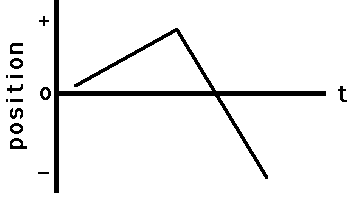
\includegraphics{Images/CC/P-Graphs/4.1e/Images/Kinematics/graph24}

Graph of Question 24%
\end{minipage}}

25. Sketch a position-time graph for an object which moves in the
+ direction at a fast constant speed and then in a - direction at
a slow constant speed. 

Answer : A position-time graph for an object which moves in the +
direction at a fast constant speed and then in a - direction at a
slow constant speed is shown below. The object must first have a +
slope (corresponding to its + velocity) then it must have a - slope
(corresponding to its - velocity). Initially, the slope is large (corresponding
to a large velocity) and then the slope is small (corresponding to
a small velocity).

\doublebox{\begin{minipage}[t]{0.9\columnwidth}%
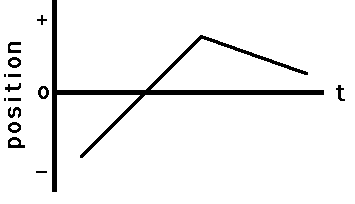
\includegraphics{Images/CC/P-Graphs/4.1e/Images/Kinematics/graph25}

Graph of Question 25%
\end{minipage}}

26. Sketch a position-time graph for an object which moves in the
- direction at a slow constant speed and then in a + direction at
a fast constant speed. 

Answer : A position-time graph for an object which moves in the -
direction at a slow constant speed and then in a + direction at a
fast constant speed is shown below. The object must first have a -
slope (corresponding to its - velocity) then it must have a + slope
(corresponding to its + velocity). Initially, the slope is small (corresponding
to a small velocity) and then the slope is large (corresponding to
a large velocity).

\doublebox{\begin{minipage}[t]{0.9\columnwidth}%
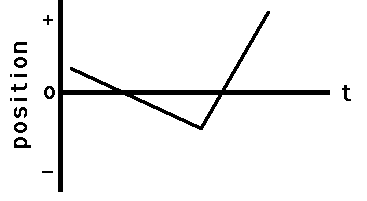
\includegraphics{Images/CC/P-Graphs/4.1e/Images/Kinematics/graph26}

Graph of Question 26%
\end{minipage}}

27. Sketch a velocity-time graph for an object moving with a constant
speed in the positive direction. 

Answer : A velocity-time graph for an object moving with a constant
speed in the positive direction is shown below. To have \textquotedbl a
constant speed in the positive direction\textquotedbl{} is to have
a + velocity which is unchanging. Thus, the line on the graph will
be in the + region of the graph (above 0). Since the velocity is unchanging,
the line is horizontal. Since the slope of a line on a v-t graph is
the object's acceleration, a horizontal line (zero slope) on a v-t
graph is characteristic of a motion with zeo acceleration (constant
velocity).

\doublebox{\begin{minipage}[t]{0.9\columnwidth}%
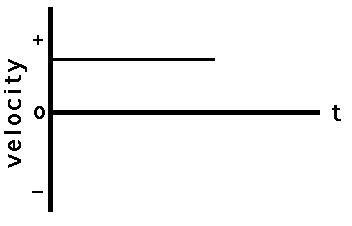
\includegraphics{Images/CC/P-Graphs/4.1e/Images/Kinematics/graph27}

Graph of Question 27%
\end{minipage}}

28. Sketch a velocity-time graph for an object moving with a constant
speed in the negative direction. 

Answer : A velocity-time graph for an object moving with a constant
speed in the negative direction is shown below. To have \textquotedbl a
constant speed in the negative direction\textquotedbl{} is to have
a - velocity which is unchanging. Thus, the line on the graph will
be in the - region of the graph (below 0). Since the velocity is unchanging,
the line is horizontal. Since the slope of a line on a v-t graph is
the object's acceleration, a horizontal line (zero slope) on a v-t
graph is characteristic of a motion with zeo acceleration (constant
velocity).

\doublebox{\begin{minipage}[t]{0.9\columnwidth}%
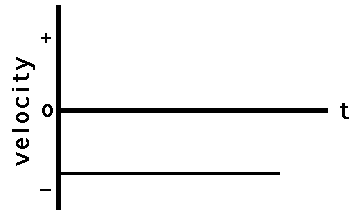
\includegraphics{Images/CC/P-Graphs/4.1e/Images/Kinematics/graph28}

Graph of Question 28%
\end{minipage}}

29. Sketch a velocity-time graph for an object which is at rest. 

Answer : A velocity-time graph for an object which is at rest is shown
below. To be \textquotedbl at rest\textquotedbl{} is to have a zero
velocity. Thus the line is drawn along the axis (v=0).

\doublebox{\begin{minipage}[t]{0.9\columnwidth}%
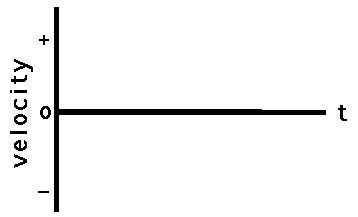
\includegraphics{Images/CC/P-Graphs/4.1e/Images/Kinematics/graph29}

Graph of Question 29%
\end{minipage}}

30. Sketch a velocity-time graph for an object moving in the + direction,
accelerating from a slow speed to a fast speed. 

Answer : A velocity-time graph for an object moving in the + direction,
accelerating from a slow speed to a fast speed is shown below. An
object which is moving in the + direction and speeding up (slow to
fast) has a + acceleration. (If necessary, review the dir'n of the
acceleration vector in the Physics Classroom Tutorial.) Since the
slope of a line on a v-t graph is the object's acceleration, an object
with + acceleration is represented by a line with + slope. Thus, the
line is a straight diagonal line with upward (+) slope. Since the
velocity is +, the line is plotted in the + region of the v-t graph.

\doublebox{\begin{minipage}[t]{0.9\columnwidth}%
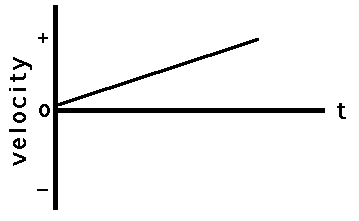
\includegraphics{Images/CC/P-Graphs/4.1e/Images/Kinematics/graph30}

Graph of Question 30%
\end{minipage}}

31. Sketch a velocity-time graph for an object moving in the + direction,
accelerating from a fast speed to a slow speed. 

Answer : A velocity-time graph for an object moving in the + direction,
accelerating from a fast speed to a slow speed is shown below. An
object whgich is moving in the + direction and slowing down (fast
to slow) has a - acceleration. (If necessary, review the dir'n of
the acceleration vector in the Physics Classroom Tutorial.) Since
the slope of a line on a v-t graph is the object's acceleration, an
object with - acceleration is represented by a line with - slope.
Thus, the line is a straight diagonal line with downward (-) slope.
Since the velocity is +, the line is plotted in the + region of the
v-t graph.

\doublebox{\begin{minipage}[t]{0.9\columnwidth}%
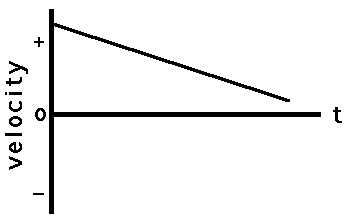
\includegraphics{Images/CC/P-Graphs/4.1e/Images/Kinematics/graph31}

Graph of Question 31%
\end{minipage}}

32. Sketch a velocity-time graph for an object moving in the - direction,
accelerating from a slow speed to a fast speed.

Answer : A velocity-time graph for an object moving in the - direction,
accelerating from a slow speed to a fast speed is shown below. An
object whgich is moving in the - direction and speeding up (slow to
fast) has a - acceleration. (If necessary, review the dir'n of the
acceleration vector in the Physics Classroom Tutorial.) Since the
slope of a line on a v-t graph is the object's acceleration, an object
with - acceleration is represented by a line with - slope. Thus, the
line is a straight diagonal line with downward (-) slope. Since the
velocity is -, the line is plotted in the - region of the v-t graph.

\doublebox{\begin{minipage}[t]{0.9\columnwidth}%
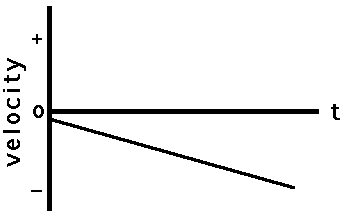
\includegraphics{Images/CC/P-Graphs/4.1e/Images/Kinematics/graph32}

Graph of Question 32%
\end{minipage}}

33. Sketch a velocity-time graph for an object moving in the - direction,
accelerating from a fast speed to a slow speed. 

Answer : A velocity-time graph for an object moving in the - direction,
accelerating from a fast speed to a slow speed is shown below. An
object whgich is moving in the - direction and slowing down (fast
to slow) has a + acceleration. (If necessary, review the dir'n of
the acceleration vector in the Physics Classroom Tutorial.) Since
the slope of a line on a v-t graph is the object's acceleration, an
object with + acceleration is represented by a line with + slope.
Thus, the line is a straight diagonal line with upward (+) slope.
Since the velocity is -, the line is plotted in the - region of the
v-t graph.

\doublebox{\begin{minipage}[t]{0.9\columnwidth}%
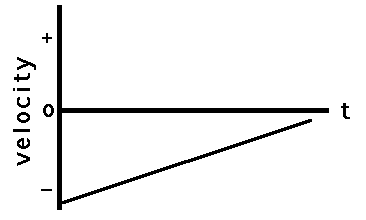
\includegraphics{Images/CC/P-Graphs/4.1e/Images/Kinematics/graph33}

Graph of Question 33%
\end{minipage}}

34. Sketch a velocity-time graph for an object which first moves with
a slow, constant speed in the + direction, and then with a fast constant
speed in the + direction.

Answer : A velocity-time graph for an object which first moves with
a slow, constant speed in the + direction, and then with a fast constant
speed in the + direction is shown below. Since there are two parts
of this object's motion, there will be two distinct parts on the graph.
Each part is in the + region of the v-t graph (above 0) since the
velocity is +. Each part is horizontal since the velocity during each
part is constant (constant velocity means zero acceleration which
means zero slope). The second part of the graph will be higher since
the velocity is greater during the second part of the motion.

\doublebox{\begin{minipage}[t]{0.9\columnwidth}%
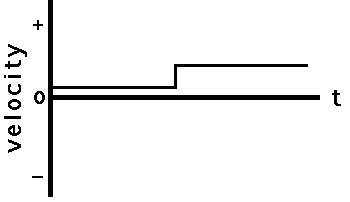
\includegraphics{Images/CC/P-Graphs/4.1e/Images/Kinematics/graph34}

Graph of Question 34%
\end{minipage}}

35. Sketch a velocity-time graph for an object which first moves with
a fast, constant speed in the + direction, and then with a slow constant
speed in the + direction. 

Answer : A velocity-time graph for an object which first moves with
a fast, constant speed in the + direction, and then with a slow constant
speed in the + direction is shown below. Since there are two parts
of this object's motion, there will be two distinct parts on the graph.
Each part is in the + region of the v-t graph (above 0) since the
velocity is +. Each part is horizontal since the velocity during each
part is constant (constant velocity means zero acceleration which
means zero slope). The first part of the graph will be higher since
the velocity is greater during the first part of the motion.

\doublebox{\begin{minipage}[t]{0.9\columnwidth}%
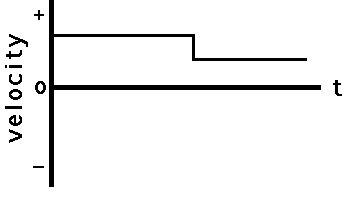
\includegraphics{Images/CC/P-Graphs/4.1e/Images/Kinematics/graph35}

Graph of Question 35%
\end{minipage}}

36. Sketch a velocity-time graph for an object which first moves with
a constant speed in the + direction, and then moves with a positive
acceleration. 

Answer : A velocity-time graph for an object which first moves with
a constant speed in the + direction, and then moves with a positive
acceleration is shown below. Since there are two parts of this object's
motion, there will be two distinct parts on the graph. Each part is
in the + region of the v-t graph (above 0) since the velocity is +.
The slope of the first part is zero since constant velocity means
zero acceleration and zero acceleration is represented by a horizontal
line on a v-t graph (slope = acceleration for v-t graphs). The second
part of the graph is an upward sloping line since the object has +
acceleration (again, the slope = acceleration for v-t graphs)

\doublebox{\begin{minipage}[t]{0.9\columnwidth}%
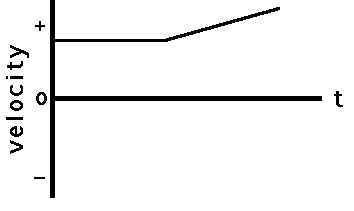
\includegraphics{Images/CC/P-Graphs/4.1e/Images/Kinematics/graph36}

Graph of Question 36%
\end{minipage}}

37. Sketch a velocity-time graph for an object which first moves with
a constant speed in the + direction, and then moves with a negative
acceleration. 

Answer : A velocity-time graph for an object which first moves with
a constant speed in the + direction, and then moves with a negative
acceleration is shown below. Since there are two parts of this object's
motion, there will be two distinct parts on the graph. Each part is
in the + region of the v-t graph (above 0) since the velocity is +.
The slope of the first part is zero since constant velocity means
zero acceleration and zero acceleration is represented by a horizontal
line on a v-t graph (slope = acceleration for v-t graphs). The second
part of the graph is an downward sloping line since the object has
- acceleration (again, the slope = acceleration for v-t graphs) 

\doublebox{\begin{minipage}[t]{0.9\columnwidth}%
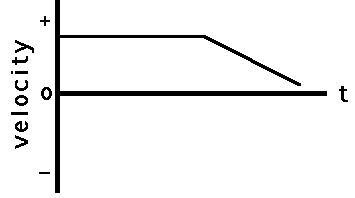
\includegraphics{Images/CC/P-Graphs/4.1e/Images/Kinematics/graph37}

Graph of Question 37%
\end{minipage}}

\section{Exercises}

Example : Which position-versus-time graph represents the motion shown
in the motion diagram?

\doublebox{\begin{minipage}[t]{0.72\columnwidth}%
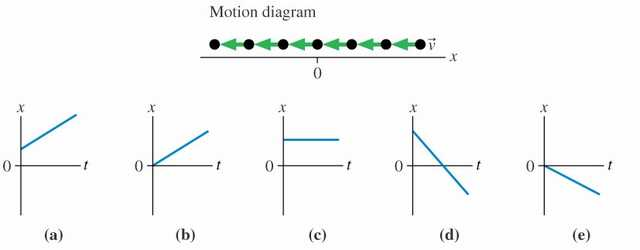
\includegraphics[scale=0.5]{Images/CC/P-Graphs/4.1e/Images/Kinematics/image7}%
\end{minipage}}

Solution : 

\doublebox{\begin{minipage}[t]{0.72\columnwidth}%
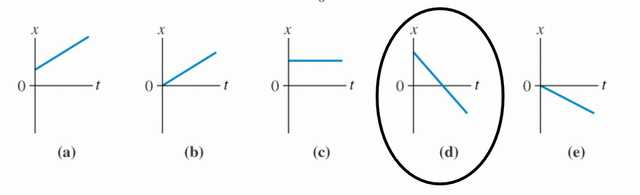
\includegraphics[scale=0.5]{Images/CC/P-Graphs/4.1e/Images/Kinematics/image7_sol}%
\end{minipage}}

\strong{Example} : Which velocity-versus-time graph goes with this
position-versus-time graph on the left?

\doublebox{\begin{minipage}[t]{0.72\columnwidth}%
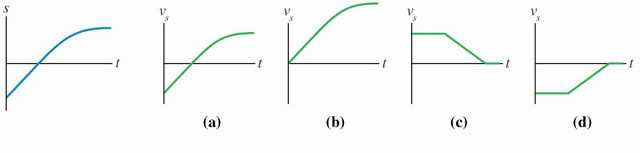
\includegraphics[scale=0.5]{Images/CC/P-Graphs/4.1e/Images/Kinematics/q_2}%
\end{minipage}}

Note that the variable \textquotedblleft s\textquotedblright{} denotes
a generic Cartesian coordinate. It could be x or y.

Solution : 

\doublebox{\begin{minipage}[t]{0.72\columnwidth}%
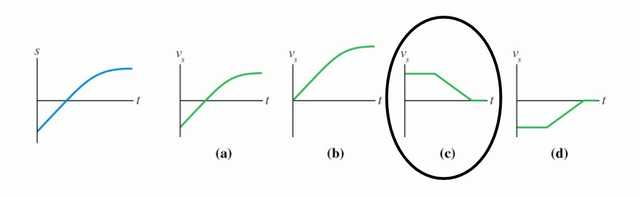
\includegraphics[scale=0.5]{Images/CC/P-Graphs/4.1e/Images/Kinematics/q_2_ans}%
\end{minipage}}

The velocity graph must match the slope of the position graph. The
position graph starts with a constant positive slope. Then the slope
decreases to zero.

\strong{Example} : Which position-versus-time graph goes with this
velocity-versus-time graph on the left? The particle\textquoteright s
position at ti = 0 s is xi = \textendash 10 m .

\doublebox{\begin{minipage}[t]{0.72\columnwidth}%
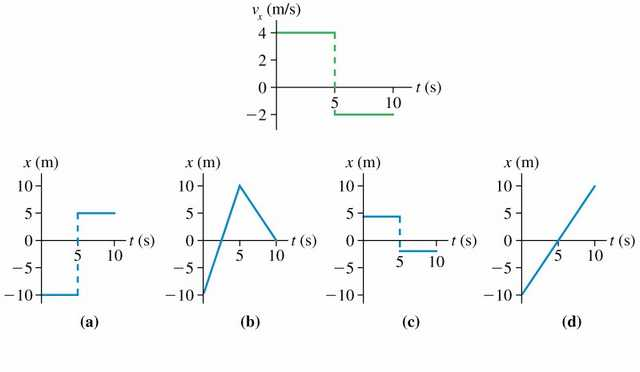
\includegraphics[scale=0.5]{Images/CC/P-Graphs/4.1e/Images/Kinematics/q3}%
\end{minipage}}

Solution : 

\doublebox{\begin{minipage}[t]{0.72\columnwidth}%
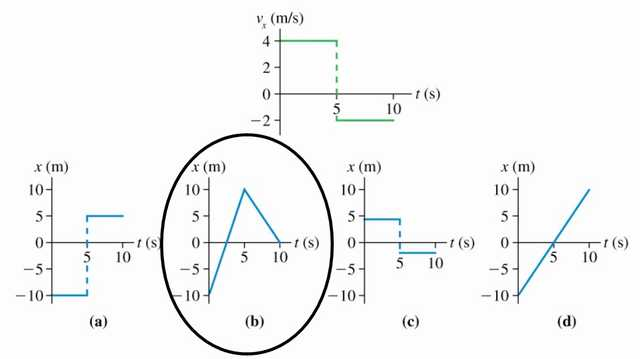
\includegraphics[scale=0.5]{Images/CC/P-Graphs/4.1e/Images/Kinematics/q3_ans}%
\end{minipage}}

The velocity graph must match the slope of the position graph. The
intercept of the position graph is arbitrary.

\strong{Example} : Which velocity-versus-time graph or graphs goes
with this acceleration-versus-time graph? The particle is initially
moving to the right and eventually to the left.

\doublebox{\begin{minipage}[t]{0.72\columnwidth}%
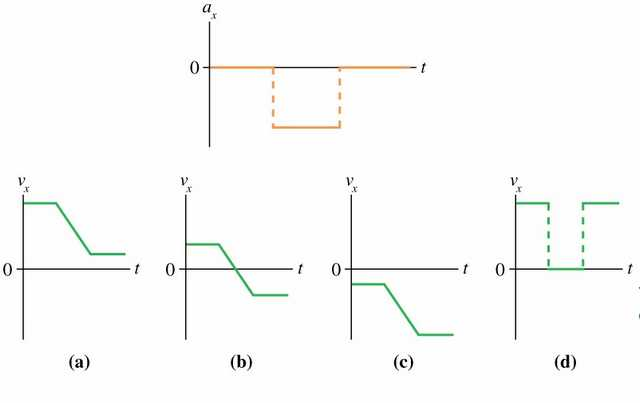
\includegraphics[scale=0.5]{Images/CC/P-Graphs/4.1e/Images/Kinematics/q4}%
\end{minipage}}

Solution : 

\doublebox{\begin{minipage}[t]{0.72\columnwidth}%
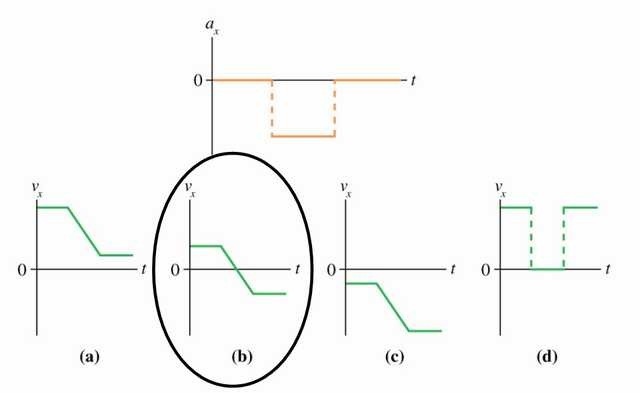
\includegraphics[scale=0.5]{Images/CC/P-Graphs/4.1e/Images/Kinematics/q4_ans}%
\end{minipage}}

The slope of the velocity graph must match the acceleration graph.
The intercept is based on the direction information.

\strong{Example} : The ball rolls up the ramp, then back down. Which
is the correct acceleration graph?

\doublebox{\begin{minipage}[t]{0.72\columnwidth}%
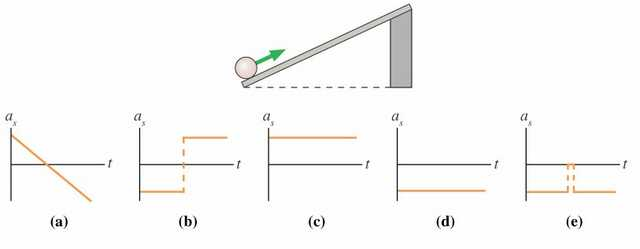
\includegraphics[scale=0.5]{Images/CC/P-Graphs/4.1e/Images/Kinematics/q5}%
\end{minipage}}

Solution : 

\doublebox{\begin{minipage}[t]{0.72\columnwidth}%
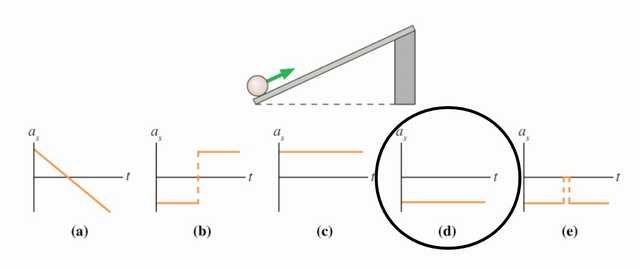
\includegraphics[scale=0.5]{Images/CC/P-Graphs/4.1e/Images/Kinematics/q5_ans}%
\end{minipage}}

The ball will move up the ramp while slowing down, then it will reach
a turnaround point and begin to move down the ramp with increasing
speed. The velocity graph at right is consistent with that description.
The acceleration graph shown in graph d is consistent with the requirement
that it match the slope of the velocity graph.

\strong{Example} : An expectant father paces back and forth producing
the potison-versus-time graph shown here. 

(a) Without performing a calculation indicate whether the father\textquoteright s
velocity is positive, negative, or zero on the segments of the graph
labeled A, B, C, and C. 

\doublebox{\begin{minipage}[t]{0.72\columnwidth}%
\includegraphics[scale=0.5]{\string"Images/CC/P-Graphs/4.1e/Images/Kinematics/Kinematics Graphs1\string".jpg}%
\end{minipage}}

Segment A: 

Segment B: 

Segment C: 

Segment D: 

(b) Calculate the average velocity for each segment and show that
your results verify your answers to part (a). 

Segment A: 

Segment B: 

Segment C: 

Segment D: 

Example : 2. A motorcycle moves according to the velocity-versus-time
graph shown. Find the displacement of the motorcycle for each of the
segments A, B, and C. 

\doublebox{\begin{minipage}[t]{0.72\columnwidth}%
\includegraphics[scale=0.5]{\string"Images/CC/P-Graphs/4.1e/Images/Kinematics/KinematicGraphs-Class Exercise\string".jpg}%
\end{minipage}}

Segment A: 

Segment B: 

Segment C: 

\strong{Example} : Fig. shows the displacement-time graph of a car
during parking. Describe the motion of the car and find the velocity
in each time interval.\cite{www.hk-phy.org}

\doublebox{\begin{minipage}[t]{0.72\columnwidth}%
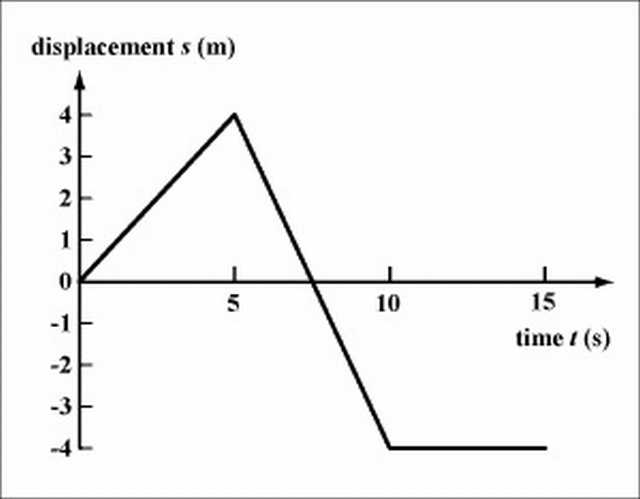
\includegraphics[scale=0.5]{Images/CC/P-Graphs/4.1e/Images/Kinematics/5-02}%
\end{minipage}}

\strong{Solution}: Stage 1: The car moves forwards from the origin
to s=4m in the first 5 s.

v=4/5=0.8m/s (forwards)

Stage 2: The car moves backwards, passes the origin, to s=-4m in the
next 5 s.

v=(-4-4)/(10-5)=-1.6m/s (backwards)

Stage 3: The car remains at rest in the last 5 s.

v=0m/s

\strong{Example} : Fig. is the displacement-time graph for a car
encountering a traffic light. Describe the motion of the car at each
stage qualitatively.\cite{www.hk-phy.org}

\doublebox{\begin{minipage}[t]{0.72\columnwidth}%
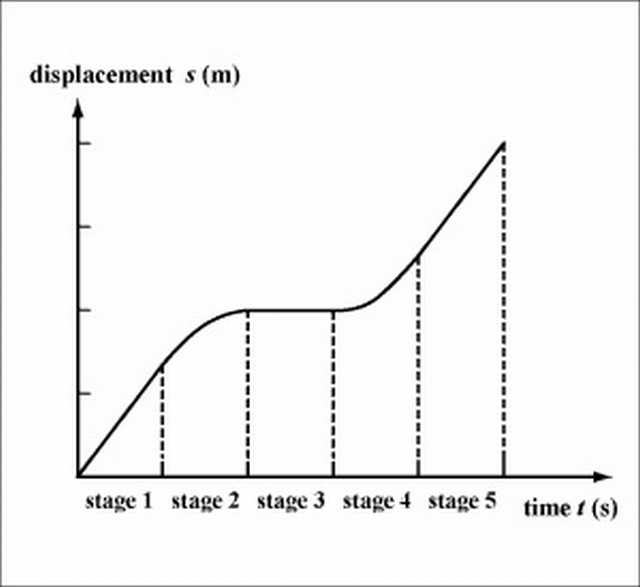
\includegraphics[scale=0.5]{Images/CC/P-Graphs/4.1e/Images/Kinematics/5-03}%
\end{minipage}}

\strong{Solution} : Stage 1: moving with constant velocity; stage
2: decelerating; stage 3: at rest; stage 4: accelerating; stage 5:
moving with the same constant velocity as in stage 1.

Note: In stage 2 the slope of the curve is decreasing, while in stage
4 the slope is increasing. This indicates that the car is decelerating
in stage 2 and accelerating in stage 4.

\strong{Example} : An object's position during a given time interval
is shown by the graph below:

\doublebox{\begin{minipage}[t]{0.72\columnwidth}%
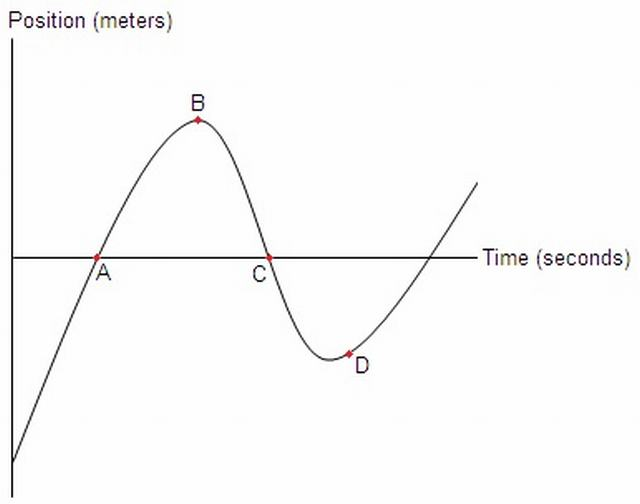
\includegraphics[scale=0.5]{Images/CC/P-Graphs/4.1e/Images/Kinematics/ex24}%
\end{minipage}}

a.) At which of the marked points is the object's velocity the greatest?
The least? 

b.) Is the object's acceleration positive or negative between points
A and B? 

c.) Suppose this curve can be modeled by the function x(t) = t3 -
9.5t2 + 23t - 9. Find the object's velocity and acceleration at t
= 1, t = 3, and t = 5. 

d.) Using the function from part c, determine the object's maximum
and minimum positions and velocities within the interval from t =
1 to t = 6.

\strong{Solution} : a.) Remember from problem 22 that velocity is
the slope of a position vs. time graph such as this. By looking at
lines tangent to the curve, we can see which point has the highest
and lowest slope:

\doublebox{\begin{minipage}[t]{0.72\columnwidth}%
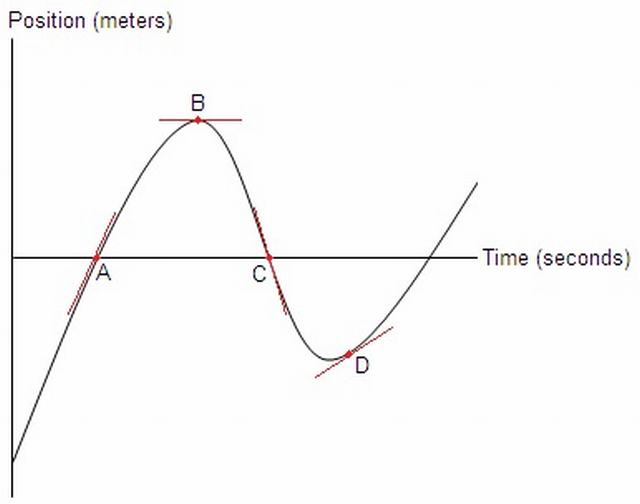
\includegraphics[scale=0.5]{Images/CC/P-Graphs/4.1e/Images/Kinematics/ex24a}%
\end{minipage}}

Looking at the red tangent lines, we can immediately eliminate point
B as a candidate for both the maximum and minimum velocity, as its
tangent is horizontal and thus has a slope of 0. Point C is the only
marked point whose tangent line has a negative slope, so point C has
the lowest velocity. Looking at points A and D, point A's tangent
line has a steeper positive slope so point A has the highest velocity.

b.) We know that acceleration is a change in velocity, so by asking
whether acceleration is positive or negative, we are asking if the
velocity is increasing or decreasing. Since velocity is the slope
of this graph, we must determine how the slope of the curve is changing
between points A and B. Looking at the diagram in part a, we see that
the slope at point A is positive, and the slope at point B is 0. As
such, the slope, and thus the velocity, must be decreasing. Therefore,
the object's acceleration is negative in this interval.

c.) We know from problem 22 that velocity is the derivative of position,
and from problem 23 that acceleration is the derivative of velocity.
So, we will begin by differentiating the position function twice:
x(t) = t3 - 9.5t2 + 23t - 9 v(t) = 3t2 - 19t + 23 a(t) = 6t - 19

Now that we know the velocity and acceleration functions, all that
is left is to plug the values of t into these functions and simplify:
v(1) = 3 {*} 12 - 19 {*} 1 + 23 = 3 - 19 + 23 = 7 m/s v(3) = 3 {*}
32 - 19 {*} 3 + 23 = 27 - 57 + 23 = -7 m/s v(5) = 3 {*} 52 - 19 {*}
5 + 23 = 75 - 95 + 23 = 3 m/s

a(1) = 6 {*} 1 - 19 = 6 - 19 = -13 m/s2 a(3) = 6 {*} 3 - 19 = 18 -
19 = -1 m/s2 a(5) = 6 {*} 5 - 19 = 30 - 19 = 11 m/s2

d.) Thinking logically about the graph, the possible candidates for
maximum and minimum position are at the end points of the interval
and at the spots, like point B, where the slope of the graph is 0.
So, first we set the velocity function from part c equal to 0 and
solve for t: v(t) = 3t2 - 19t + 23 = 0 t = 1.63008 s or t = 4.70326
s

Note that this was solved using a graphing calculator. The AP exam
will not ask you to solve a quadratic this complicated by hand, however
you may have to solve a simpler function using the quadratic formula.
Also, we keep as many decimal places as we can at this stage in order
to maintain accuracy. Now that we know all the possible times at which
the position could be at a maximum or minimum within the interval,
we simply plug these t values into x(t). Don't forget to check the
end points: x(t) = t3 - 9.5t2 + 23t - 9 x(1) = 5.5 m x(1.63008) =
7.58 m x(4.70326) = -6.93 m x(6) = 3 m

We see that the minimum position is -6.93 m, and the maximum position
is 7.58 m. Finding the maximum and minimum velocities is achieved
in the same manner, except we set the acceleration function equal
to 0 and plug the t values into the velocity funtion: a(t) = 6t -
19 = 0 6t = 19 t = 19/6 = 3.16667 s

v(t) = 3t2 - 19t + 23 v(1) = 7 m/s v(3.16667) = -7.08 m/s v(6) = 17
m/s

So the minimum velocity is -7.08 m/s, and the maximum velocity is
17 m/s.

\chapter{Classical Approach}

\section{The Equations of motion and the origin of Graph Handling}

\subsection{\index{The First Equation}The First Equation}

The Equation $v=\dfrac{dx}{dt}$ in linear motion implies
\begin{quote}
i) The \textbf{Slope} of \textbf{Position-Time Graph} is \textbf{Instantaneous
Velocity.}

ii) The \textbf{Area} under the \textbf{Velocity-Time Graph} is \textbf{Change
in Position}.

\{ The second one requires the manipulation , $dx=vdt$ i.e. $\int dx=\int vdt$
\} 
\end{quote}
The equations can be further manipulated to obtain the Speed Time
Graph , where 
\begin{quotation}
speed = rate of change of distance wrt time 
\end{quotation}
Few of the following examples illustrate this concept: 
\begin{description}
\item [{\strong{\textbf{Example 1}}:}] On a displacement-time graph, two
straight lines make angles of 30� and 60� with the time-axis. The
ratio of the velocities represented by them is 
\end{description}
\begin{quote}
a) $1:\sqrt{3}$

b) 1:3

c) $\sqrt{3}:1$

d) 3:1

\{ Hint: The velocity in a displacement-time is given by the slope
of the curve. Slope = tan(gent) of angle of inclination of s-t graph.
This gives the respective ratios tan 30$^{o}$ / tan 60$^{o}$ 

Answer: b) is the correct answer. \}
\end{quote}
\begin{description}
\item [{\strong{\textbf{Example 2}}:}] A body is moving in a straight
line as shown in velocity-time graph. The displacement and distance
travelled by body in 8 second are respectively:
\end{description}
\doublebox{\begin{minipage}[t]{0.7\columnwidth}%
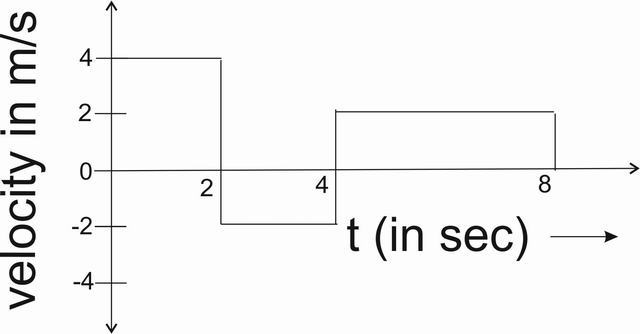
\includegraphics[scale=0.5]{Images/CC/P-Graphs/4.1e/Images/KinematicsClassicalApproach/ImagesReduced/Q2-firstequation}%
\end{minipage}}
\begin{quote}
a) 12 m, 20 m

b) 20 m, 12 m

c) 12 m, 12 m

d) 20 m, 20 m

\{ Hint: The displacement in a velocity-time graph is given by the
area under the graph with proper signs. From 0s - to 2s , the area
is 8m . From 2s - to 4s , the area is -4m . From 4s - to 8s , the
area is 8m. Adding these 3 values , we get 8m + (-4m) + 8m = 12m.
\} The distance in a v-t graph is given by the absolute area under
the graph. So, taking the absolute values of individual area divisions,
we get 8m + 4m + 8m =20m

Answer: a) is the correct answer. \}
\end{quote}
\begin{description}
\item [{\strong{\textbf{Example 3}}:}] The graph shows position as a function
of time for two trains running on parallel tracks. Which statement
is true?
\end{description}
\doublebox{\begin{minipage}[t]{0.7\columnwidth}%
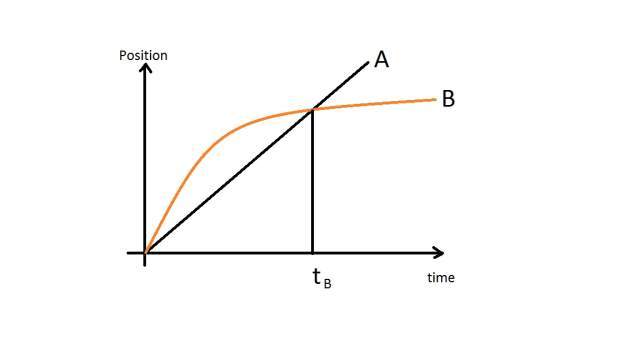
\includegraphics[scale=0.75]{Images/CC/P-Graphs/Common/Reduced/ClassicalApproach/Paralleltracktrains}%
\end{minipage}}
\begin{quote}
a) At time t$_{B}$ both trains have the same velocity.

b) Both trains have the same velocity at some time after t$_{B}$
.

c) Both trains have the same velocity at some time before t$_{B}$
.

d) Somewhere on the graph, both trains have the same acceleration.

\{ Hint: Depending on the question requirements, we'll have to check
all the assertions one by one.

a) In a position time graph, the slope gives velocity. It can be clearly
seen that Graph B has a much lower slope than Graph A at time $t_{B}$.
So, the assertion is wrong.

b,c) By drawing a line parallel to the line A which is a tangent to
Graph B , it can be seen where the two graphs have same slope. It
is clear that the graphs have same slope between 0 and $t_{B}$ as
noted from the figure. So, assertion b is wrong while c is correct.

\doublebox{\begin{minipage}[t]{0.7\columnwidth}%
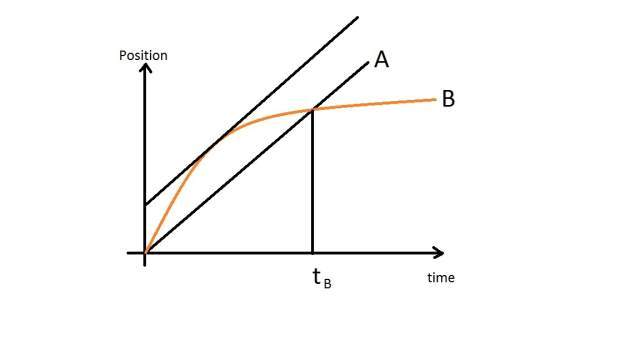
\includegraphics[scale=0.75]{Images/CC/P-Graphs/Common/Reduced/ClassicalApproach/Paralleltracktrainssolution}%
\end{minipage}}

d) As the Graph A has a constant slope, so the acceleration of body
A is zero. Whereas Graph B is constantly turning, so the slope can
be assumed to be non-zero throughout. According to some revelations,
however it is noted that the figure is not clear enough to show whether
Graph B is straight after $t_{B}$ or bending. In case it is assumed
to be straight, then after $t_{B}$ both trains will have same (zero)
acceleration. Also at start both have large (infinite) accelration,
in which case the ratio of the two large ( infinite ) values may be
calculated if initial conditions are mentioned and is required.

At our level we would assume this assertion to be wrong, however making
a note that the image should have been more clearly presented.

Answer: c) is the correct assertion. \}
\end{quote}
\textbf{\strong{\textbf{Example 4}}:} The velocity-time graph of
a particle in linear motion is as shown. Both v and t are in SI units.
The displacement of the particle is

\doublebox{\begin{minipage}[t]{0.7\columnwidth}%
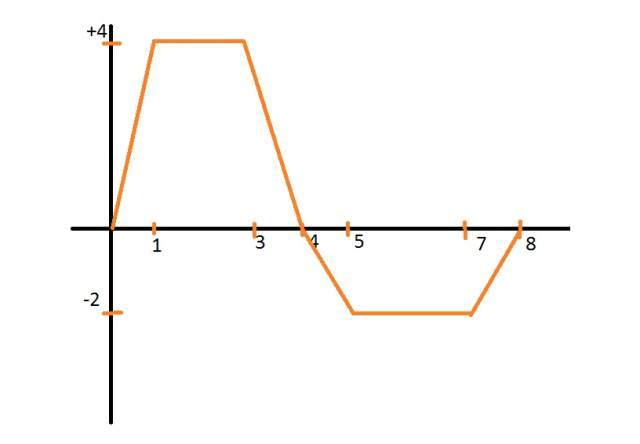
\includegraphics[scale=0.75]{Images/CC/P-Graphs/Common/Reduced/ClassicalApproach/displacementfromvtgraphproblem}%
\end{minipage}}
\begin{quote}
a) 6 m

b) 8 m

c) 16 m

d) 18 m

\{ Hint : For displacement calculations, between 0 - to 4 , area of
the positive trapesium = $\dfrac{1}{2}\times\left(2+4\right)\times4$
= 12

between 4 - to 8, area of negative trapesium =$\dfrac{1}{2}\times(2+4)\times(-2)$
= -6.

So , the answer is +6

So , a is the correct option.\}
\end{quote}
\strong{Example 5} : A speedboat starts from rest, accelerating at
2 ms$^{-2}$ for 20 s. It then continues at a steady speed for a further
30 s and decelerates to rest in 30 s. Find:

(a) the distance travelled in m,

(b) the average speed in ms $^{-1}$ and,

(c) the time taken to cover half the distance.

\doublebox{\begin{minipage}[t]{0.72\columnwidth}%
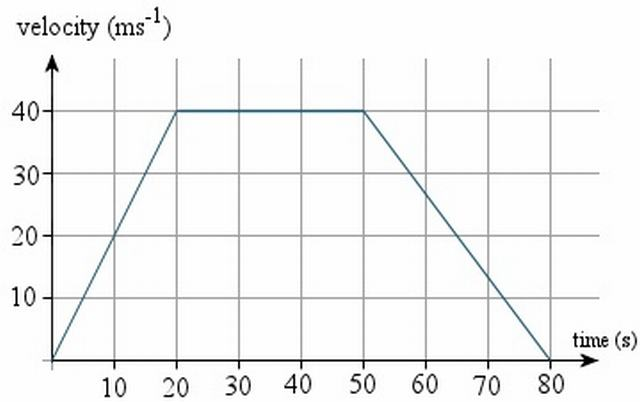
\includegraphics[scale=0.5]{Images/CC/P-Graphs/4.1e/Images/Kinematics/ex2}%
\end{minipage}}

\strong{Solution} : a) distance=area of trapezium ${\displaystyle =\frac{\left(a+b\right)h}{2}}$ 

${\displaystyle =\frac{\left(80+30\right)\left(40\right)}{2}}$ 

=2200 m

b) ${\displaystyle \text{average speed}=\frac{\text{distance travelled}}{\text{time taken}}}$

${\displaystyle =\frac{2200}{80}}$

=27.5 ms $^{-1}$

c) We need to find the time when the area of the trapezium is half
of its original area, or 1100m , as shown in the graph.

\doublebox{\begin{minipage}[t]{0.72\columnwidth}%
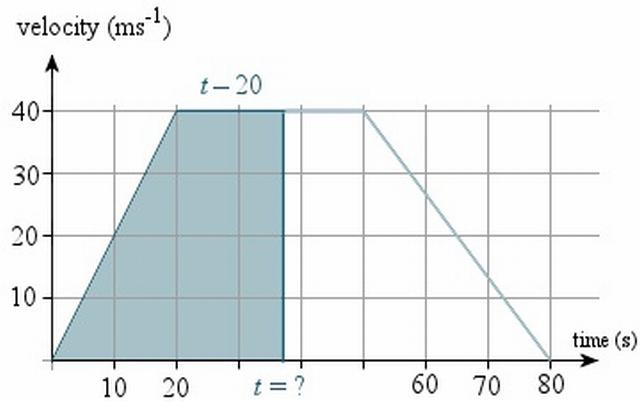
\includegraphics[scale=0.5]{Images/CC/P-Graphs/4.1e/Images/Kinematics/ex2c}%
\end{minipage}}

The base of this unknown trapezium has length \textbackslash displaystyle\{t\}t,
and the top of the trapezium will have length t\textminus 20. So we
have:

${\displaystyle \text{area of trapezium}=\frac{\left(a+b\right)h}{2}}$

${\displaystyle 1100=\frac{\left(t+\left[t-20\right]\right)40}{2}=20\left(2t-20\right)}$ 

55=2t\textminus 20 

75=2t 

t=37.5s 

So it will take 37.5 s to cover half the distance.

\subsection{\index{The Second Equation}The Second Equation}

Proceeding similar to above, the equation $a=\dfrac{dv}{dt}$ implies
\begin{quote}
i) The \textbf{Slope} of \textbf{Velocity-Time Graph} is \textbf{Instantaneous
Acceleration}.

ii) The\textbf{ Area} under \textbf{Acceleration-Time Graph} is \textbf{Change
in Velocity}.

\{ The second one requires the manipulation , $dv=adt$ i.e. $\int dv=\int adt$
\} 
\end{quote}
A few of the following examples illustrate it.
\begin{description}
\item [{\strong{Example 1}:}] A car starts from rest acquires a velocity
v with uniform acceleration $2ms^{-2}$ then it comes to stop with
uniform retardation $4ms^{-2}$ . If the total time for which it remains
in motion is 3 sec, the total distance travelled is:
\end{description}
\begin{quote}
a) 2 m

b) 3 m

c) 4 m

d) 6 m 

\{Hint: For solving this problem, we draw the graph of the problem, 

\doublebox{\begin{minipage}[t]{0.7\columnwidth}%
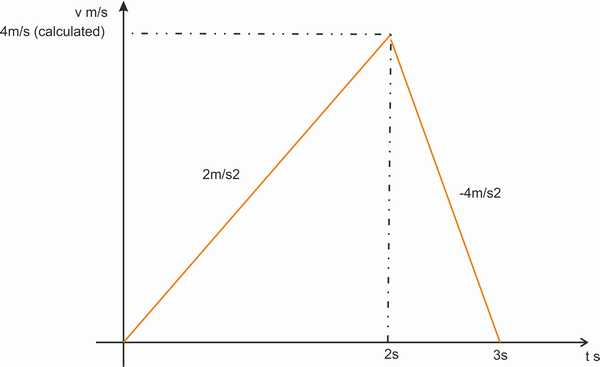
\includegraphics[scale=0.5]{Images/CC/P-Graphs/4.1e/Images/KinematicsClassicalApproach/ImagesReduced/Q1-secondequation-Answers}%
\end{minipage}} 

Accordning to graph, let the time when it reaches maximum velocity
be T, and the maximum velocity be V. 

$\Rightarrow$V = 2XT and also V = 4X(3-T)

Equating the equations,

2T = 12-4T = V

$\Rightarrow$6T = 12

$\Rightarrow$T = 2

$\Rightarrow$ V = 2T = 4

Calculating the area under the graph using the calculated parameters,
Area = 1/2 X 4 X 3 = 6m

So , area under the graph is 6m = displacement . Also, as all the
area is on the positive side, so distance = 6m. 

\}
\end{quote}
\begin{description}
\item [{\strong{Example 2}:}] A particle starts from rest. Its acceleration
(a) vs time (t) is as shown in the Figure. The maximum speed of the
particle will be
\item [{%
\doublebox{\begin{minipage}[t]{0.7\columnwidth}%
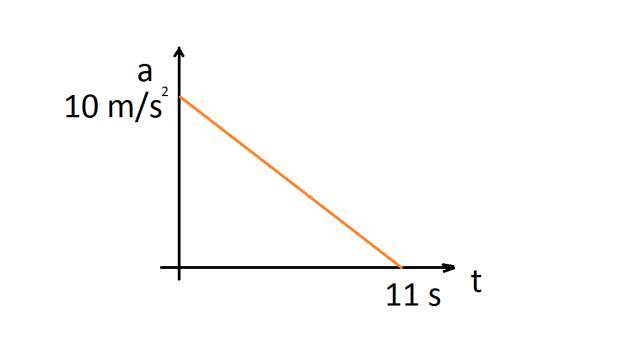
\includegraphics[scale=0.75]{Images/CC/P-Graphs/Common/Reduced/ClassicalApproach/accelerationvstime}%
\end{minipage}}}]~
\end{description}
\begin{quote}
a) 110 m/s

b) 55 m/s

c) 550 m/s

d) 660 m/s

\{ Hint : Writing the equation of the graph , we get $\dfrac{a}{10}+\dfrac{t}{11}=1$

$\Rightarrow$$a=\dfrac{10}{11}(11-t)$

Integrating, ( we will assume initial velocity to be zero as the body
starts from rest. )

$v=\dfrac{10}{11}(11t-\dfrac{1}{2}t^{2})$

Substituting $t=11s$

$v_{11s}=55m/s$

Answer: b) is the correct answer \}
\end{quote}
\begin{description}
\item [{\strong{Example 3}:}] Acceleration-time graph of a particle moving
in a straight line is shown in Figure. The velocity of particle at
time t = 0 is 2 m/s. Velocity at the end of fourth second is
\item [{%
\doublebox{\begin{minipage}[t]{0.7\columnwidth}%
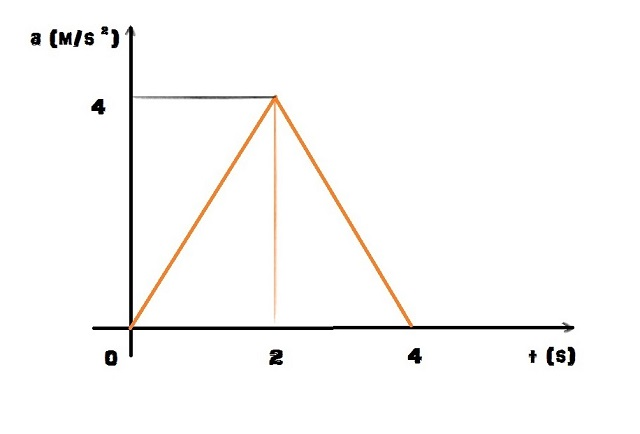
\includegraphics[scale=0.75]{Images/CC/P-Graphs/Common/Original/ClassicalApproach/acc-t-graph-3}%
\end{minipage}}}]~
\end{description}
\begin{quote}
a) 8 m/s

b) 10 m/s

c) 12 m/s

d) 14 m/s

\{ Hint: Area under the acceleration-time graph is change in velocity.
Area of the triangle is Half ( into ) base ( into ) altitude = 8m/s.
Adding the initial value of 2m/s , we get 2 + 8 = 10m/s. 

Answer: b) is the correct answer \}
\end{quote}
\begin{description}
\item [{\strong{Example 4}:}] Each of the three graphs represents acceleration
vs time for an object that already has a positive velocity at time
$t_{1}$ . Which graph/graphs show an object whose speed is increasing
for the entire time interva1 between $t_{1}$ and $t_{2}$ ?
\item [{%
\doublebox{\begin{minipage}[t]{0.7\columnwidth}%
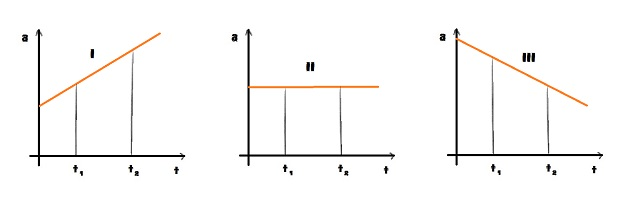
\includegraphics[scale=0.75]{Images/CC/P-Graphs/Common/Original/ClassicalApproach/ncertproblem}%
\end{minipage}}}]~
\end{description}
\begin{quote}
a) Graph I only

b) Graphs I and II

c) Graphs I and III

d) Graphs I, II and III

\{Hint: Area under the acceleration time graphs give change in velocity.
In all the three figures, the area under the graphs are +ve, hence
velocity is increasing in all cases. As the initial velocity is +ve
, in all three cases the velocity remains throughout positive. So
, the speed is also increasing in all cases.\}
\end{quote}
\begin{description}
\item [{\strong{Example 5}:}] A body starts from rest and moves along
a straight line with constant acceleration. The variation of speed
v with distance s is given by the graph
\item [{%
\doublebox{\begin{minipage}[t]{0.7\columnwidth}%
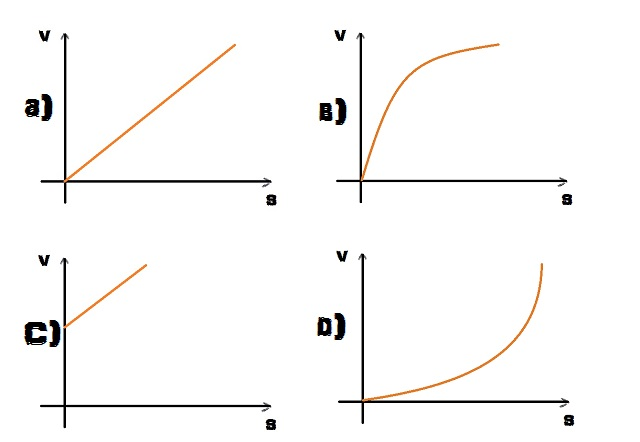
\includegraphics[scale=0.5]{Images/CC/P-Graphs/Common/Original/ClassicalApproach/Untitled2}%
\end{minipage}}}]~
\end{description}
\begin{quote}
\{ Hint: The problem given has $v_{o}$= 0 

Now acceleration = constant ( lets say k ) = $\dfrac{dv}{dt}$

$\Rightarrow$$k=v\dfrac{dv}{ds}$

$\Rightarrow$$\int_{0}^{v}vdv=\int_{0}^{s}kds$

$\Rightarrow$$v=\sqrt{2ks}$

The graph is proportional to square root function

Hence , b (as it is the only graph with such a property )

Answer : b) is the correct graph \}
\end{quote}

\subsection{The Acceleration-Position Graph Variate}
\begin{quote}
This kind of graph requires the manipulation of the Equation $a=\dfrac{dv}{dt}$
as follows

$a=\dfrac{dv}{dx}.\dfrac{dx}{dt}$

$\Rightarrow$$a=\dfrac{dv}{dx}.v$

$\Rightarrow$ $adx=vdv$ and integration can be performed to further
solve it.
\end{quote}
\begin{description}
\item [{\strong{Example 1}:}] A body, initially at rest, starts moving
along x-axis in such a way that its acceleration vs displacement plot
is as shown in the Figure. The maximum velocity of the particle is
\item [{%
\doublebox{\begin{minipage}[t]{0.7\columnwidth}%
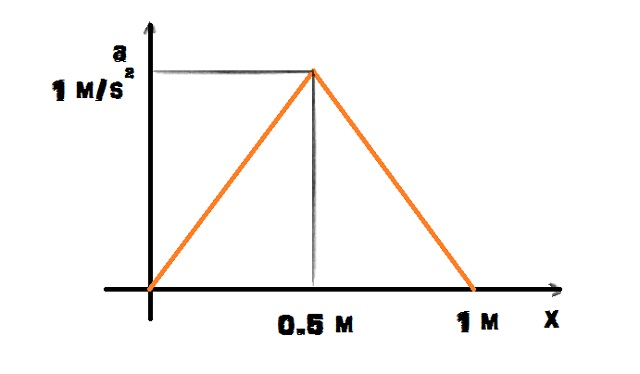
\includegraphics[scale=0.5]{Images/CC/P-Graphs/Common/Original/ClassicalApproach/accelerationposition1}%
\end{minipage}}}]~
\end{description}
\begin{quote}
a) 1 m/s

b) 6 m/s

c) 2 m/s

d) None of these

\{ Hint : The area under the a-x graph gives change in $\dfrac{v^{2}}{2}$
as can be evaluated by Integration method. The area of triange is
(0.5) X (1) X (1) = 0.5

$\Rightarrow$v = 1m/s . Initial position is given to be 0 in the
graph. Hence, we take only the positive sign.

Answer : a) is the correct answer. \}
\end{quote}
\begin{description}
\item [{\strong{Example 2}}] : A particle initially at rest, it is subjected
to a non-uniform acceleration a, as shown in the gure. The maximum
speed attained by the particle is
\item [{%
\doublebox{\begin{minipage}[t]{0.7\columnwidth}%
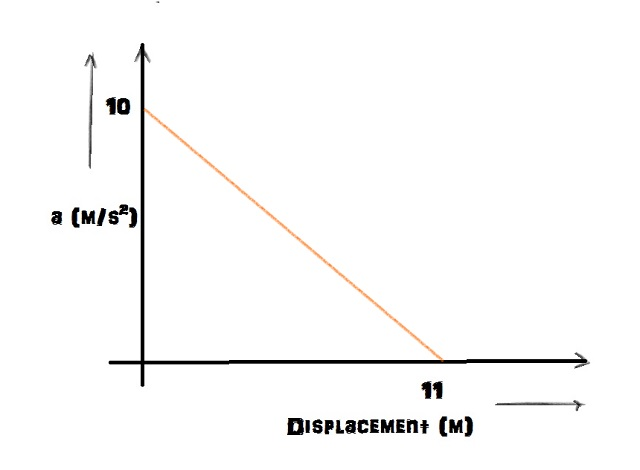
\includegraphics[scale=0.5]{Images/CC/P-Graphs/Common/Original/ClassicalApproach/acclnvsdisplacement}%
\end{minipage}}}]~
\end{description}
\begin{quote}
a) 605 m/s

b) 110 m/s

c) 55 m/s 

d) 110 m/s

\{ Hint: The answer is 55m/s as calculated in the example above(In
the second equation section). Hence, c) is the correct response.

Answer : c) is the correct answer. \}
\end{quote}

\subsection{\index{Sign of Acceleration from Position-Time Graph}Sign of Acceleration
from Position-Time Graph}
\begin{quote}
The sign of Acceleration can be determined from the Position-Time
Graph. The methodology involves of looking at the Concavity of the
Graph

i) If the graph is Concave-Up, the Acceleration is Positive.

ii) If the graph is Concave-Down, the Acceleration is Negative.

iii) If the graph is a straight line, the Acceleration is ZERO. \{
Irrespective of any other factor , such as the slope or direction
of line\} 
\end{quote}
\begin{description}
\item [{\strong{Example 1}:}] The graph given below is a plot of distance
vs time. For which labelled region is the ``Velocity Positive and
the Acceleration Negative''
\end{description}
\doublebox{\begin{minipage}[t]{0.7\columnwidth}%
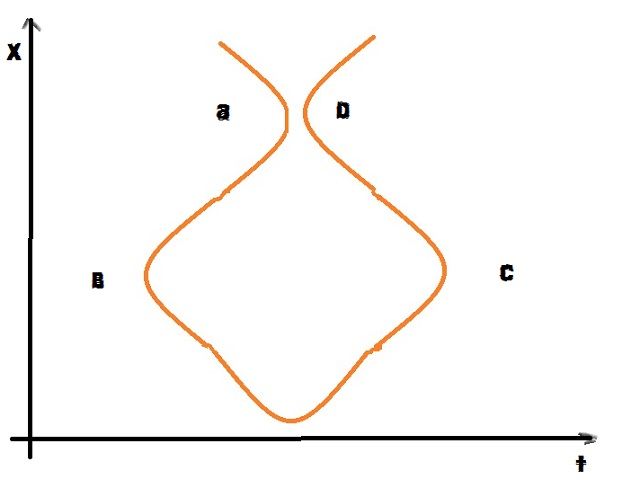
\includegraphics[scale=0.5]{Images/CC/P-Graphs/Common/Original/ClassicalApproach/signofacclnfromxt}%
\end{minipage}}
\begin{quote}
a) a

b) b

c) c

d) d 

\{ Hint: By the above mentioned propositions, d) is the required section
with positive velocity and negative accleration. \}
\end{quote}

\subsection{\index{The Average-Velocity / Instantaneous Velocity , Equal Case}The
Average-Velocity / Instantaneous Velocity , Equal Case}
\begin{quote}
We know , that ( in a x-t graph) the slope of the Secant is the Average
Velocity , whereas the slope of Tangent is the Instaneous Velocity.
The point where these two lines coincide, is the point where Average
Velocity is equal to Instantaneous Velocity.
\end{quote}
\begin{description}
\item [{\strong{Example 1}:}] Position-time graph is shown which is a
semicircle from t = 2 to t = 8 s. Find time t at which the instantaneous
velocity is equal to average velocity over first t seconds,
\end{description}
\begin{quote}
\doublebox{\begin{minipage}[t]{0.7\columnwidth}%
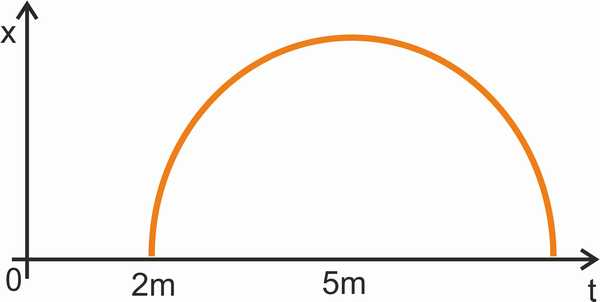
\includegraphics[scale=0.5]{Images/CC/P-Graphs/4.1e/Images/KinematicsClassicalApproach/ImagesReduced/Q1-avinseq}%
\end{minipage}}

a) 4.8 s

b) 3.2 s

c) 2.4 s

d) 5 s

\{ Hint: The tangent from 0 to the circle is drawn. It's normal passes
through the center of the circle. Time at this instant needs to be
calculated.

If H=5 , R = 3 , Length of tangent = 4. (By Pythagoras.)

Angle which the tangent makes with the t axis is $\theta$ = $sin^{-1}(3/5)$

So, the projection of tangent on t axis ( i.e. the required time )
= 4 cos $\theta$ = $4\times\dfrac{4}{5}=3.2$

\doublebox{\begin{minipage}[t]{0.7\columnwidth}%
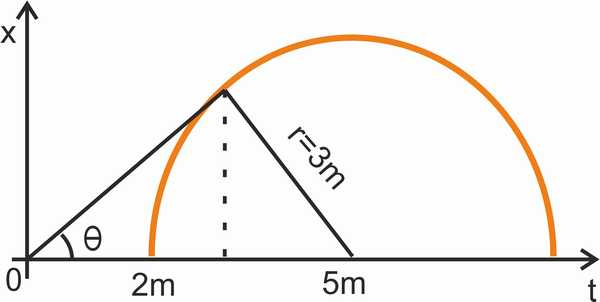
\includegraphics[scale=0.5]{Images/CC/P-Graphs/4.1e/Images/KinematicsClassicalApproach/ImagesReduced/Q1-avinseq-Answer}%
\end{minipage}}

\}
\end{quote}

\subsection{The Velocity-Displacement Case}
\begin{quote}
This can be handled in a similar way as Acceleration-Displacement
case by integrating the respective equation. Here the problem is of
v = f(x) type, which can be integrated by writing $\dfrac{dx}{dt}=f(x)$

i.e. dx = f(x)dt
\end{quote}
\begin{description}
\item [{\strong{Example 1}:}] The velocity-displacement graph of a particle
moving along a straight line is shown here.
\item [{%
\doublebox{\begin{minipage}[t]{0.7\columnwidth}%
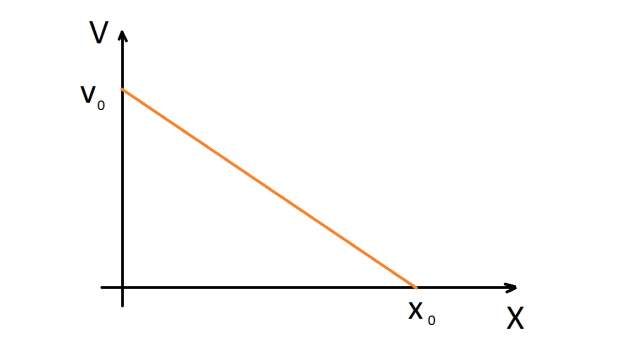
\includegraphics[scale=0.75]{Images/CC/P-Graphs/Common/Reduced/ClassicalApproach/velocitydisplacement}%
\end{minipage}}}]~
\end{description}
\begin{quote}
The most suitable acceleration-displacement graph will be

\doublebox{\begin{minipage}[t]{0.7\columnwidth}%
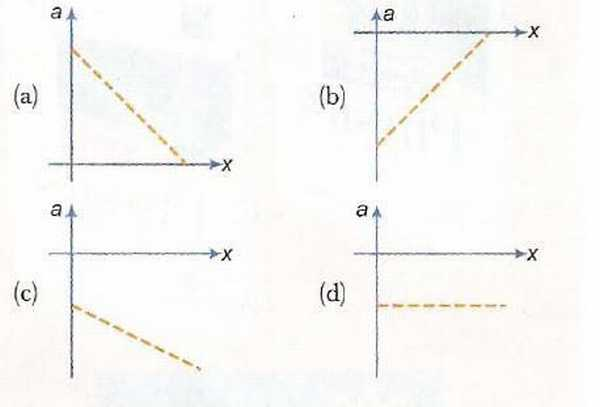
\includegraphics[scale=0.5]{Images/CC/P-Graphs/4.1e/Images/KinematicsClassicalApproach/ImagesReduced/Q1-velocitydisplacementanswer}%
\end{minipage}}

\{Hint: Using Co-Ordinate Geometry Result studied in +1 Mathematics,
we get the equation of the graph

$\dfrac{v}{v_{o}}+\dfrac{x}{x_{o}}=1$

We are supposed to find the a-x graph from this.

So, we rewrite this equation as $v=v_{o}(1-\dfrac{x}{x_{o}})$

Differentiating, we get $a=-\dfrac{v_{o}}{x_{o}}v=-\dfrac{v_{o}^{2}}{x_{o}}(1-\dfrac{x}{x_{o}})$

Hence b) is the requisite graph, the only graph with a +ve slope ,
a negative y intercept and a positive x intercept.

Answer: b) is the correct answer. \} \footnote{The problem has been solved wrong in the Extended First Edition and
Third Edition released earlier this month. The date is 23-March-2017
today, as of this writing. So, a useful Errata.}
\end{quote}
\begin{description}
\item [{\strong{Example 2}:}] The velocity (v) of a body moving along
the postive x-direction varies with displacement (x) from the origin
as p v = k x , where k is a constant. Which of the graphs shown in
Fig. correctly represents the displacement-time (x - t) graph of the
motion?
\item [{%
\doublebox{\begin{minipage}[t]{0.7\columnwidth}%
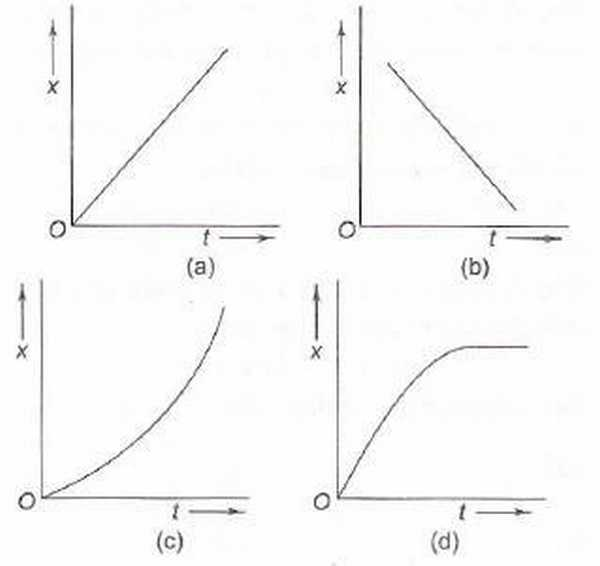
\includegraphics[scale=0.5]{Images/CC/P-Graphs/4.1e/Images/KinematicsClassicalApproach/ImagesReduced/Q2-velocitydisplacement}%
\end{minipage}}}]~
\end{description}
\begin{quote}
\{Hint: The variable p removes the dependence of v on x and gives
emphasis only on the first condition that body is moving along positive
x-direction. In Graphs a) ,c) body is moving along positive x-direction,
However, a) is a specific case when p is proportional to x and not
the general case. Only c) covers the general case of all possible
p and still moving in positive x-direction. Hence c) is the correct
answer

Answer: c) is the required answer. \}
\end{quote}

\subsection{Motion Under Free Fall\index{Motion Under Free Fall} due to Gravity}
\begin{quote}
In such examples, the governing equations rule and the coordi-nate
system needs to be properly chosen.
\end{quote}
\begin{description}
\item [{\strong{Example 1}:}] Which of the following graphs correctly
represents velocity-time relationship for a particle released from
rest to fall freely under gravity? 
\item [{%
\doublebox{\begin{minipage}[t]{0.7\columnwidth}%
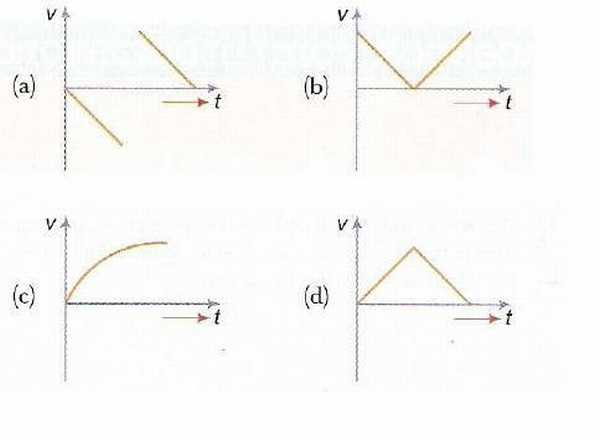
\includegraphics[scale=0.5]{Images/CC/P-Graphs/4.1e/Images/KinematicsClassicalApproach/ImagesReduced/Q2-freefall}%
\end{minipage}}}]~
\end{description}
\begin{quote}
\{ Hint: If we take the downward axis as positive, v will keep on
increasing till the object hits something. 

So, a) is the correct answer.\}
\end{quote}
\begin{description}
\item [{\strong{Example 2}:}] A body A is thrown vertically upwards with
such a velocity that it reaches a maximum height of h. Simultaneously
another body B is dropped from height h. It strikes the ground and
doesn't rebound. The velocity of A relative to B vs time graph is
best represented by (upward direction is positive.)
\item [{%
\doublebox{\begin{minipage}[t]{0.7\columnwidth}%
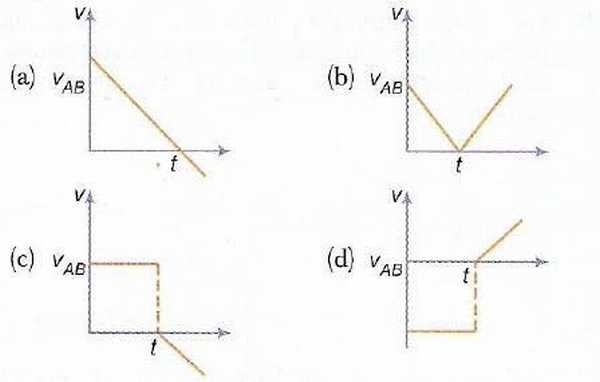
\includegraphics[scale=0.5]{Images/CC/P-Graphs/4.1e/Images/KinematicsClassicalApproach/ImagesReduced/Q3-freefall}%
\end{minipage}}}]~
\end{description}
\begin{quote}
\{ Hint: Before the strike, body A has velocity u-gt whereas body
B has velocity -gt. So, a constant difference of u remains. Before
strike, $u-gt_{o}+gt_{o}=u$ . However , after that it is u-gt , the
time being $t_{o}$=u/g of strike. So, the negative slope line starts
from the x-axis and a discontinuity comes into picture. 

So , C) is the required graph.\}
\end{quote}
\strong{Example 3} : A ball is thrown vertically downward from a
120-m high building. The ball hits the ground in 2 seconds. How fast
was the ball thrown? 

Sketches of the velocity and acceleration graphs are shown in Fig.
1. For simplicity, the downward direction is assumed to be positive,
and, for ease of calculations, the freefall acceleration g is taken
to be 10 m/s2. Knowing that the area under the acceleration graph
is equal to the change in velocity ($\triangle v$ ) of the object
yields $\triangle v$ = gt = 10 m/s$^{2}\times$ 2 s = 20 m/s. 

\doublebox{\begin{minipage}[t]{0.72\columnwidth}%
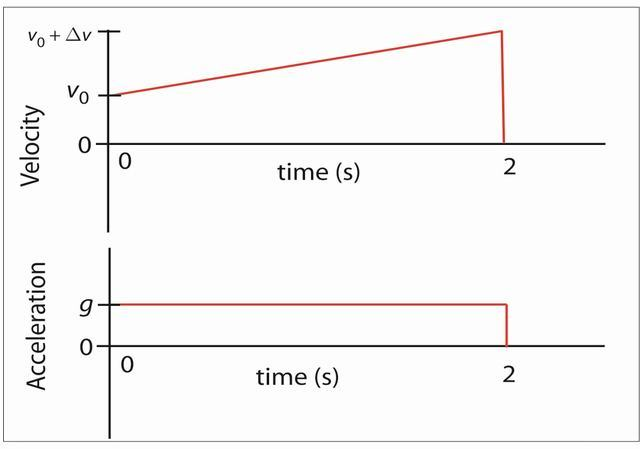
\includegraphics[scale=0.5]{Images/CC/P-Graphs/4.1e/Images/Kinematics/Untitled-1}

Velocity and acceleration graphs for Problem 1. %
\end{minipage}}

The area under the velocity graph is the displacement, which was given
to be 120 m. Breaking the area under graph into a rectangle and a
triangle yields 120 m = v0 3 t + 1 2 Dv 3 t = 2 s 3 v0 + 1 2 20 m/s
3 2 s. (2) One can easily solve this for the initial velocity of the
object, thus obtaining the answer to the problem (50 m/s is a quite
unrealistic initial velocity for a thrown ball). No explicit use of
the standard kinematic equations is made; the solution is based on
only the graphs. The above problem is relatively simple; to see the
real power of the method requires a more difficult 1-D kinematics
problem. 

\strong{Example 4} : Determined to test gravity, a student walks
off the cN Tower in Toronto, which is 553 m high, and falls freely.
His initial velocity is zero. The rocketeer arrives at the roof of
the building 5 seconds later to save the student. The rocketeer leaves
the roof with an initial velocity downward and then is in freefall.
in order both to catch the student and to prevent injury to him, the
rocketeer should catch the student at a sufficiently great height
and arrive at the ground with zero velocity. The upward acceleration
that accomplishes this is provided by the rocketeer\textquoteright s
jet pack, which he turns on just as he catches the student; before
then the student is in freefall. To prevent discomfort to the student,
the magnitude of the acceleration is limited to five times gravity.
How high above the ground must the rocketeer catch the student? 

\strong{Solution} : As I was grading the assignment, one student\textquoteright s
solution stuck out. When I first saw it, I was convinced that something
must be wrong as the problem had been difficult for me and could not
be that simple. I was wrong. The simple solution consists of sketching
the velocity and acceleration graphs for the falling student (Fig.
2; down is taken as the positive direction) and using a bit of reasoning.
Since the overall change in the student\textquoteright s velocity
during his motion is zero, the total area under the acceleration-versus-time
graph must equal zero. This area consists of a positive part (above
the time axis) and a negative part (below the time axis). The two
rectangular areas must have equal magnitude, and since their heights
differ by a factor of 5, so must their widths (the two corresponding
times). Therefore, the freefall time is five times longer than the
time for slow-down to rest. Now, looking at the velocity graph, the
area labeled 1 corresponds to the displacement while in freefall,
and the area labeled 2 represents the displacement after the Rocketeer
has caught the student. The triangles forming areas 1 and 2 have the
same height, and the base (time) for area 1 is five times the base
(time) for area 2. Therefore, area 1 must be five times larger than
area 2. This means that area 2 must be 1/6 the total height of the
building, or 92.2 m. 

\doublebox{\begin{minipage}[t]{0.72\columnwidth}%
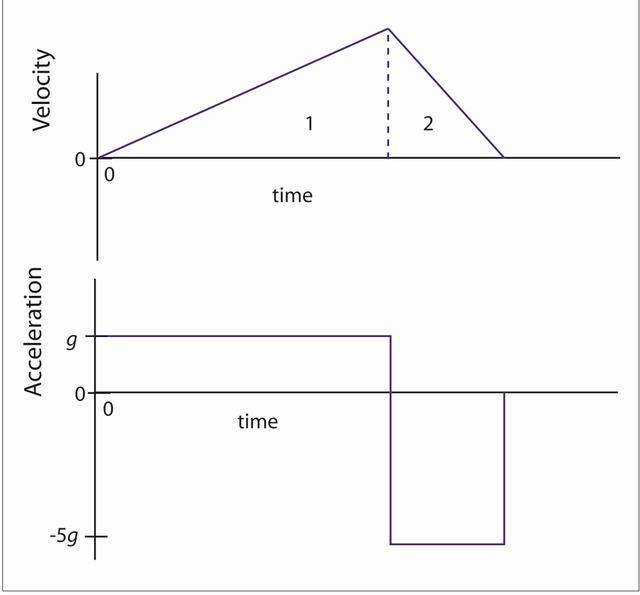
\includegraphics[scale=0.5]{Images/CC/P-Graphs/4.1e/Images/Kinematics/DesbienDwain_graphsTPT08}

Velocity and acceleration graphs for Problem 2.%
\end{minipage}}

After studying this solution for a long time and finding no flaws
in the physics, I pulled out my physics book and tried solving other
one-dimensional kinematics problems in a similar manner. It quickly
became obvious that they could be done using graphs, and in most cases
this is the easier method. I was hooked and began teaching one-dimensional
problem solving this way in all my classes. The next class period
I asked the student whose solution this was why he chose to do the
problem this way. He explained that we had emphasized graphs so much
in class that they must be more useful than something we are simply
supposed to sketch for the problems. I was amazed and appreciative
as I now had a new way to teach problem solving. This kind of solution
is more visual and helps get students away from hunting for the \textquotedblleft correct
equation.\textquotedblright{} It has worked well for me at all levels
of introductory physics, conceptual through calculus based. If you
find other interesting problems that are especially suited to the
above method, I would appreciate your sharing them. 

\subsection{Projectile Motion}
\begin{description}
\item [{\strong{Example 1}:}] A shell is fired from a gun at an angle
to the horizontal. Graphs are drawn for its horizontal component of
velocity $v_{x}$ and its vertical component of velocity $v_{y}$.
\item [{%
\doublebox{\begin{minipage}[t]{0.7\columnwidth}%
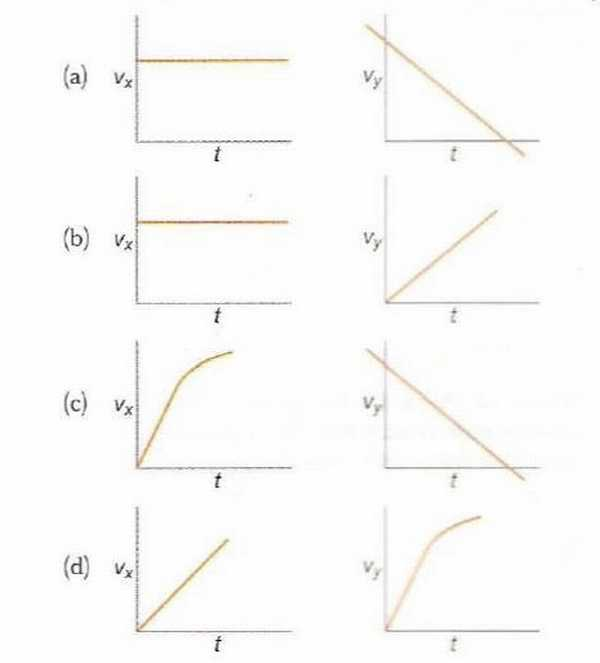
\includegraphics[scale=0.5]{Images/CC/P-Graphs/4.1e/Images/KinematicsClassicalApproach/ImagesReduced/Q4-freefall}%
\end{minipage}}}]~
\end{description}
\begin{quote}
\{ Hint: $v_{x}$ would remain constant as ucos$\theta$ and $v_{y}$
would linearly decrease and go negative after maximum height is attained(if
the fire angle is +ve).

So, a) is the requisite graph.\}
\end{quote}

\subsection{Miscelleneous}
\begin{description}
\item [{\strong{Example 1}:}] Figure shows the displacement-time ( x-t
) graph of body moving in a straight line. Which one of the graphs
shown in Fig. represents the velocity- time ( v-t ) graph of the motion
of the body.
\item [{%
\doublebox{\begin{minipage}[t]{0.7\columnwidth}%
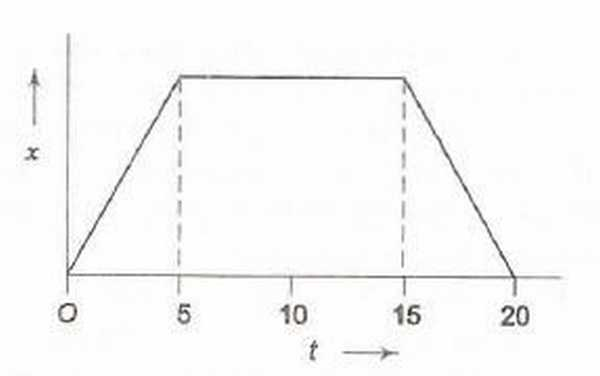
\includegraphics[scale=0.5]{Images/CC/P-Graphs/4.1e/Images/KinematicsClassicalApproach/ImagesReduced/Q1-miscelleneous}%
\end{minipage}}}]~
\item [{%
\doublebox{\begin{minipage}[t]{0.7\columnwidth}%
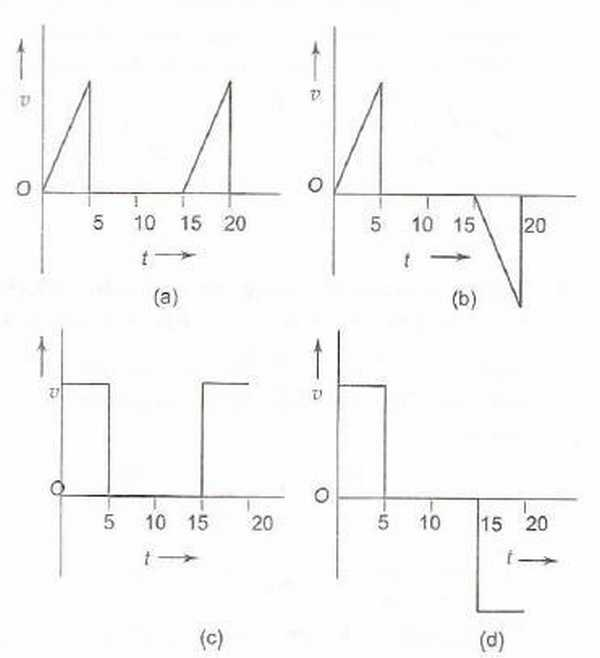
\includegraphics[scale=0.5]{Images/CC/P-Graphs/4.1e/Images/KinematicsClassicalApproach/ImagesReduced/Q1-miscelleneous-Answers}%
\end{minipage}}}]~
\end{description}
\begin{quote}
\{ Hint: The graph has initially (0-5) a +ve slope, then zero slope
and then (15-20) an equal -ve slope

So, d) is the correct answer. \}
\end{quote}
\begin{description}
\item [{\strong{Example 2}:}] Which of the displacement-time (x\textminus t)
graphs shown in Fig. can possibly represent one dimensional motion
of a particle?
\item [{%
\doublebox{\begin{minipage}[t]{0.7\columnwidth}%
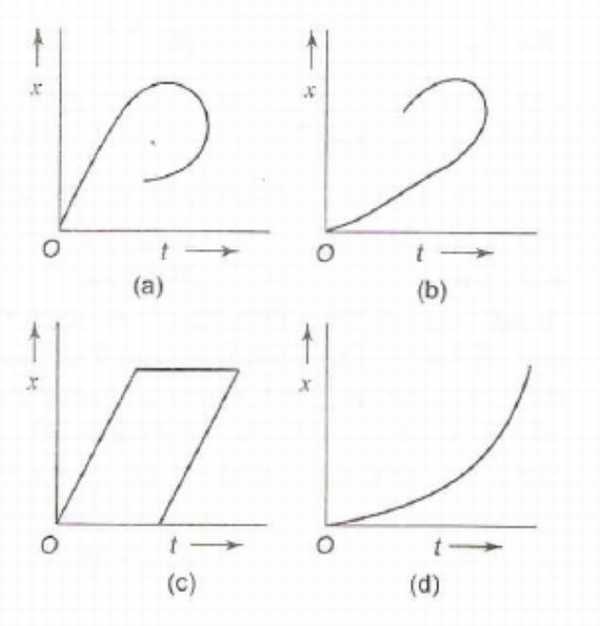
\includegraphics[scale=0.5]{Images/CC/P-Graphs/4.1e/Images/KinematicsClassicalApproach/ImagesReduced/Q2-miscelleneous}%
\end{minipage}}}]~
\end{description}
\begin{quote}
\{ Hint: The object cannot be at two positions on a single time instant,

So, d) is the correct option. \}
\end{quote}
\begin{description}
\item [{\strong{Example 3}:}] A car starts from rest, accelerates uniformly
for 4 seconds and then moves with uniform velocity. Which of the (x-t)
graphs shown in Fig. represents the motion of the car upto t = 7 s?
\item [{%
\doublebox{\begin{minipage}[t]{0.7\columnwidth}%
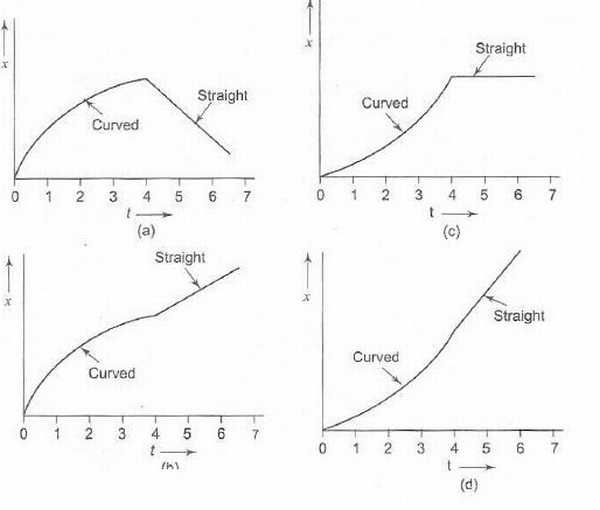
\includegraphics[scale=0.5]{Images/CC/P-Graphs/4.1e/Images/KinematicsClassicalApproach/ImagesReduced/Q3-miscelleneous}%
\end{minipage}}}]~
\end{description}
\begin{quote}
\{ Hint: As the car is accelerating upto 4 seconds, the graph should
be concave up. Further ahead , it moves with constant velocity , so
a positive slope ahead of 4 seconds. 

d) is the correct answer. \}
\end{quote}
\begin{description}
\item [{\strong{Example 4}:}] Two stones are thrown up simultaneously
with initial speeds of $u_{1}$ and $u_{2}$, ($u_{2}$ \textgreater{}
$u_{1}$) . They hit the ground after 6 s and 10 s respectively. Which
graph in Fig. correctly represents the time variation of $\triangle x=x_{2}-x_{1}$,
the relative position of the second stone with respect to the first
upto t = 10 s? Assume that the stones do not rebound after hitting
the ground.
\item [{%
\doublebox{\begin{minipage}[t]{0.7\columnwidth}%
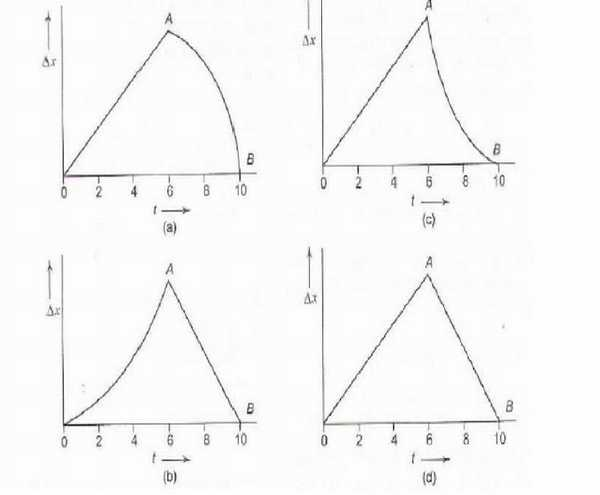
\includegraphics[scale=0.5]{Images/CC/P-Graphs/4.1e/Images/KinematicsClassicalApproach/ImagesReduced/Q4-miscelleneous}%
\end{minipage}}}]~
\end{description}
\begin{quote}
\{ Hint : While both are in air, the differece of their velocity vectors
would be a constant vector , so $\triangle x=c_{1}t$ . Also, after
the first stone hits ground, $\triangle x=c_{2}t-x_{o}$ as the velocity
component in x direction of second stone is constant. There is no
discontinutiy. So, both before and after one hits the ground , it
would be a straight line. 

Hence, d) is the correct answer. \}
\end{quote}
\begin{description}
\item [{\strong{Example 5}:}] Figure shows the velocity-time (v - t) graphs
for one dimensional motion. But only some of these can be realized
in practice. These are
\item [{%
\doublebox{\begin{minipage}[t]{0.7\columnwidth}%
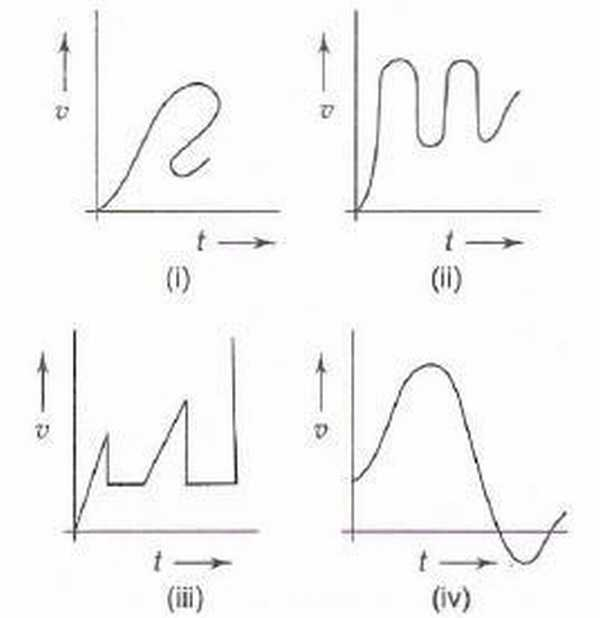
\includegraphics[scale=0.5]{Images/CC/P-Graphs/4.1e/ImagesReduced/Q5-miscelleneous}%
\end{minipage}}}]~
\end{description}
\begin{quote}
a) (i), (ii) and (iv) only

b) (i), (ii) and (iii) only

c) (ii) and (iv) only

d) all

\{ Hint: At one particular instant, the object cannot have two different
velocities. 

Hence, c) is the correct answer. \}
\end{quote}
\begin{description}
\item [{\strong{Example 6}:}] Which of the velocity-time (v-t) graphs
shown in Fig. can possibly represent one-dimensional motion of a particle?
\item [{%
\doublebox{\begin{minipage}[t]{0.7\columnwidth}%
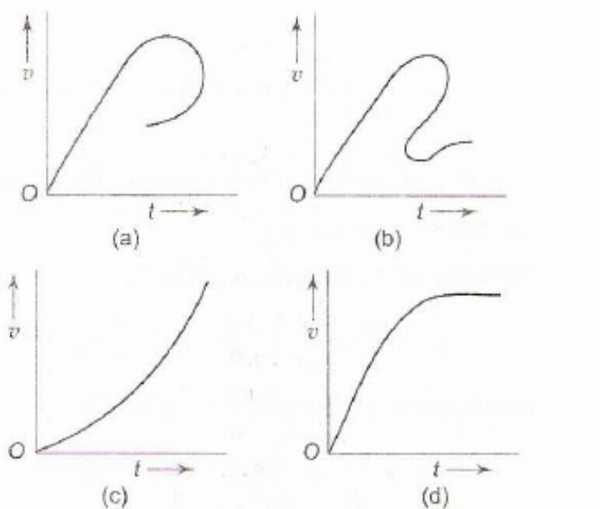
\includegraphics[scale=0.5]{Images/CC/P-Graphs/4.1e/Images/KinematicsClassicalApproach/ImagesReduced/Q6-miscelleneous}%
\end{minipage}}}]~
\end{description}
\begin{quote}
\{Hint: In c) , the particle is constantly increasing in one dimension,
In d) , it stops near the end.

c),d) are the correct answers. \}
\end{quote}

\section{Question Types}

\subsection{Passage Type}
\begin{description}
\item [{Example:}] The speed-time graph of the motion of a body is shown
in Fig.
\item [{%
\doublebox{\begin{minipage}[t]{0.7\columnwidth}%
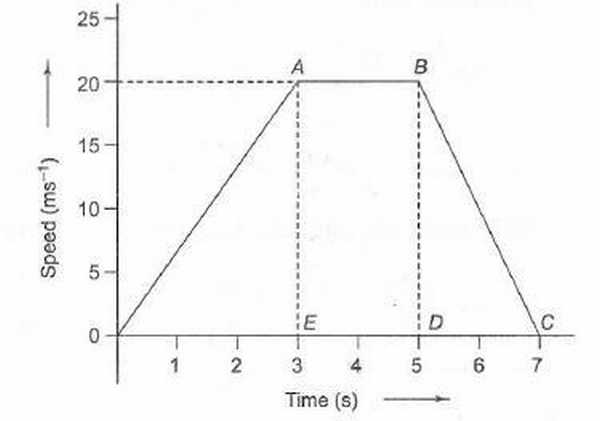
\includegraphics[scale=0.5]{Images/CC/P-Graphs/4.1e/Images/KinematicsClassicalApproach/ImagesReduced/Q1-passagetype}%
\end{minipage}}}]~
\item [{1.}] The accelerations of the body during the last 2 second is 
\end{description}
\begin{quote}
a) $\dfrac{20}{3}ms^{-2}$

b) $-\dfrac{20}{7}ms^{-2}$

c) $-10ms^{-2}$

d) Zero
\end{quote}
\begin{description}
\item [{2.}] The ratio of distance travelled by the body during the last
2 seconds to the total distance travelled by it is 
\end{description}
\begin{quote}
a) 1/9 

b) 2/9 

c) 3/9 

d) 4/9
\end{quote}
\begin{description}
\item [{3.}] The average speed of the car during the whole journey is 
\end{description}
\begin{quote}
a) 10 m/s 

b) 20 m/s 

c) 90/7 m/s 

d) 40/7 m/s 

\{Hint: 1. As no contradictory statements are present, we would take
velocity as the value of speed only. Actually velocity is required
for calculation of acceleration but here , speed doesn't contradict
anything so we'll use it's value for velocity.

-10 from slope, c)

2. Speed time graph's area is distance. From area calculation, in
last 2 seconds, the area is 20 and total area is 90. 

So, 2/9 is the required ration b)

3. Total distance from area is 90, and total time is 7. 

So, 90/7. c)\}
\end{quote}
\begin{description}
\item [{Example:}] A body starts from rest at time t = 0 and undergoes
an acceleration as shown in Fig.Which of the graphs shown in Fig.
represents the velocity-time (v-t) graph of the motion of the body
from t = 0 s to t = 4 s? 
\item [{%
\doublebox{\begin{minipage}[t]{0.7\columnwidth}%
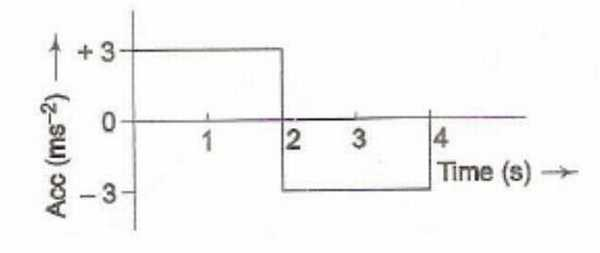
\includegraphics[scale=0.5]{Images/CC/P-Graphs/4.1e/Images/KinematicsClassicalApproach/ImagesReduced/Q2-passagetype_im1}%
\end{minipage}}}]~
\item [{%
\doublebox{\begin{minipage}[t]{0.7\columnwidth}%
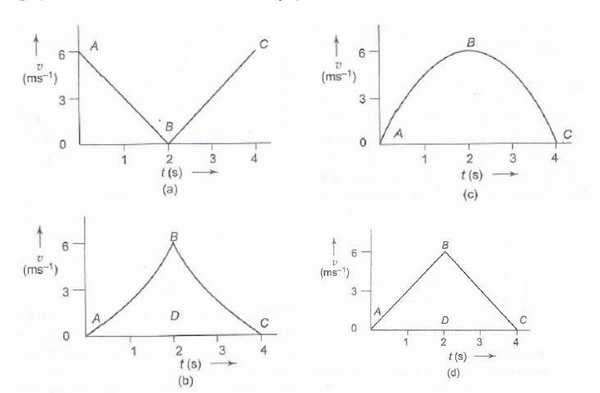
\includegraphics[scale=0.5]{Images/CC/P-Graphs/4.1e/Images/KinematicsClassicalApproach/ImagesReduced/Q2-passagetype_im2}%
\end{minipage}}}]~
\end{description}
\begin{quote}
\{Hint: d) is the v-t graph by calculating area function.\}
\end{quote}
\begin{description}
\item [{1.}] In Question above, what is the velocity of the body at time
t = 2.5 s?
\end{description}
\begin{quote}
a) 2.5 m/s

b) 3.5 m/s

c) 4.5 m/s

d) 5.5 m/s
\end{quote}
\begin{description}
\item [{2.}] In above question, how much distance does the body cover from
t = 0 s to t = 4 s?
\end{description}
\begin{quote}
a) 6 m

b) 9 m

c) 12 m

d) 15 m
\end{quote}
\begin{description}
\item [{3}] In above question, which of the graphs shown in Fig. represents
the displacement-time (x-t) graph of the motion of the body from t
= 0 s to t = 4 s?
\item [{%
\doublebox{\begin{minipage}[t]{0.7\columnwidth}%
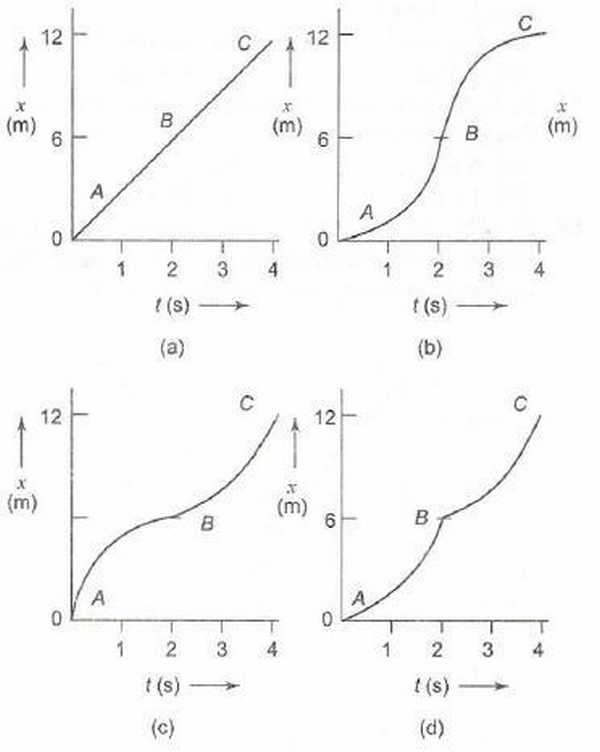
\includegraphics[scale=0.5]{Images/CC/P-Graphs/4.1e/Images/KinematicsClassicalApproach/ImagesReduced/Q2-passagetype-Answers}%
\end{minipage}}}]~
\end{description}
\begin{quote}
\{ Hint: 1. The area under the accln-time graph gives change in velocity.
Till 2.5s, 6-1.5=4.5 is the required area. 

So, c)

2. Area under the v-t graph d) is 12 till 4 seconds. 

So, c)

3. Till 2 seconds , the graph should be concave-up while from 2 to
4 it should be concave-down.

So, b)

\}
\end{quote}

\subsection{Matching}
\begin{description}
\item [{1.}] Match the graphs (a), (b), (c) and (d) shown in Fig. with
the types of motions (p), (q), (r) and (s) that they represent
\item [{%
\doublebox{\begin{minipage}[t]{0.7\columnwidth}%
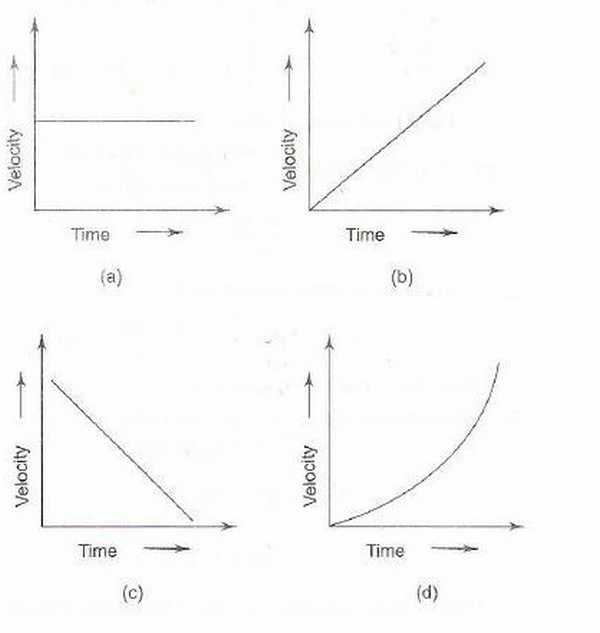
\includegraphics[scale=0.5]{Images/CC/P-Graphs/4.1e/Images/KinematicsClassicalApproach/ImagesReduced/Q1-matchingtype}%
\end{minipage}}}]~
\end{description}
\begin{quote}
p) Motion with non-uniform acceleration

q) Motion of a body covering equal distances in equal intervals of
time

r) Motion having a constant retardation

s) Uniformly accelerated motion.

\{ Hint: p-\textgreater d , q-\textgreater a, r -\textgreater c
, s-\textgreater a,b,c \}
\end{quote}
\begin{description}
\item [{2.}] Figure shows the displacement �time (x - t) graph of the m-tion
of a body.
\item [{%
\doublebox{\begin{minipage}[t]{0.7\columnwidth}%
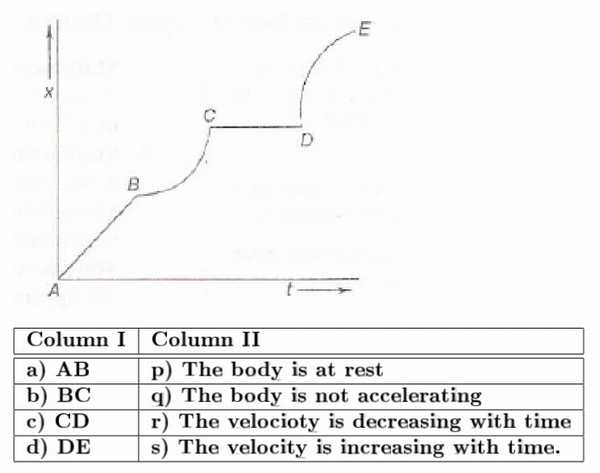
\includegraphics[scale=0.5]{Images/CC/P-Graphs/4.1e/Images/KinematicsClassicalApproach/ImagesReduced/Q2-matchingtype}%
\end{minipage}}}]~
\item [{\{}] Hint p-\textgreater c, q-\textgreater a,c, r-\textgreater{}
d , s-\textgreater b \}
\end{description}

\section{\index{Previous Years IIT Problems}Previous Years IIT Problems}
\begin{description}
\item [{Q1:}] A particle starts from rest. Its acceleration ( a ) versus
time ( t ) is as shown in the gure. The maximum speed of the particle
will be
\item [{%
\doublebox{\begin{minipage}[t]{0.7\columnwidth}%
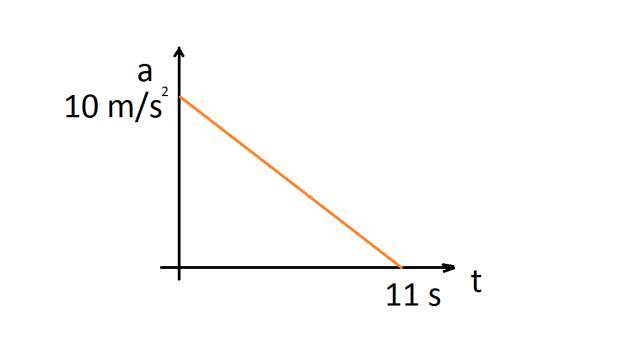
\includegraphics[scale=0.75]{Images/CC/P-Graphs/Common/Reduced/ClassicalApproach/accelerationvstime}%
\end{minipage}}}]~
\end{description}
\begin{quote}
a ) 110 m /s 

b ) 55 m /s 

c ) 550 m /s 

d ) 660 m /s

\{ Hint : See In chapter examples for solution. \}
\end{quote}
\begin{description}
\item [{Q2:}] If graph of velocity vs. distance is as shown, which of the
following graphs correctly represents the variation of acceleration
with displacement ?
\item [{%
\doublebox{\begin{minipage}[t]{0.7\columnwidth}%
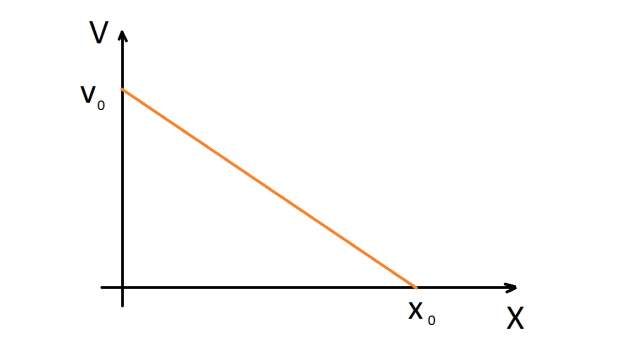
\includegraphics[scale=0.75]{Images/CC/P-Graphs/Common/Reduced/ClassicalApproach/velocitydisplacement}%
\end{minipage}}}]~
\item [{%
\doublebox{\begin{minipage}[t]{0.7\columnwidth}%
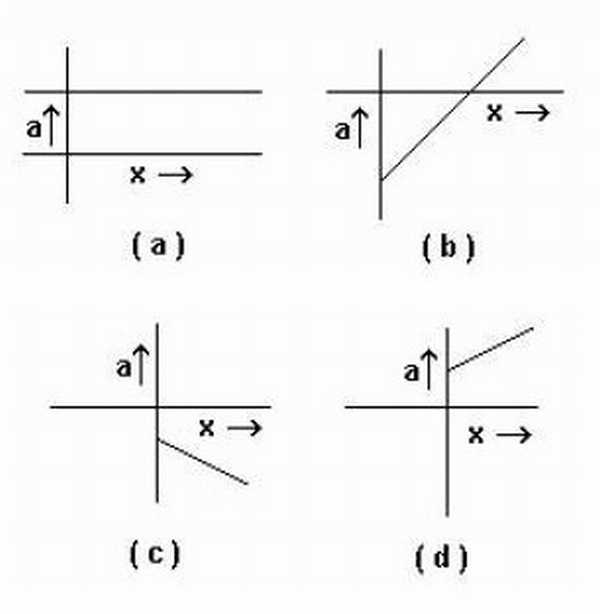
\includegraphics[scale=0.5]{Images/CC/P-Graphs/4.1e/Images/KinematicsClassicalApproach/ImagesReduced/Q2-previousyearsiit_2}%
\end{minipage}}}]~
\end{description}
\begin{quote}
\{ Hint : The graph of the question is a straight line with the equation,
$\dfrac{x}{x_{o}}+\dfrac{v}{v_{o}}=1$ 

This gives , $v=v_{o}(1-x/x_{o})$

So, diffrentiating it, we get

$a=-v_{o}/x_{o}$ which is a constant. Only in a) it is shown to be
a constant. 

So, a) \}
\end{quote}
\begin{description}
\item [{Passage}] A lift is going up. The variation in the speed of the
lift is as given in the graph. 
\item [{%
\doublebox{\begin{minipage}[t]{0.7\columnwidth}%
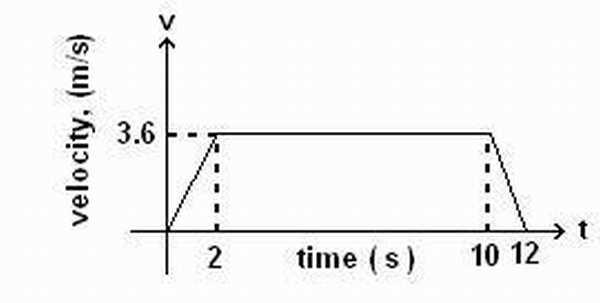
\includegraphics[scale=0.5]{Images/CC/P-Graphs/4.1e/Images/KinematicsClassicalApproach/ImagesReduced/passage-previousyearsiit}%
\end{minipage}}}]~
\item [{Q3:}] What is the height to which the lift takes the passengers
? 
\end{description}
\begin{quote}
a ) 3.6 m 

b ) 28.8 m 

c ) 36 m

d ) cannot be calculated from the above graph
\end{quote}
\begin{description}
\item [{Q4:}] In the above graph, what is the average velocity of the lift? 
\end{description}
\begin{quote}
a ) 1 m/s 

b ) 2.88 m/s

c ) 3.24 m/s 

d ) 3 m/s 
\end{quote}
\begin{description}
\item [{Q5:}] In the above graph , what is the average acceleration of
the lift? 
\end{description}
\begin{quote}
a ) 1.8$m/s^{2}$ 

b ) \textminus 1.8$m/s^{2}$ 

c ) 0.3$m/s^{2}$ 

d ) zero 

\{Hint: Q3: Area under the graph is 36. Taking initial position as
zero, c) is the best fit answer.

Q4. For av. velocity, total displacement / total time should be calculated.
which is 36/12 = 3m/s . d ) is the required answer.

Q5. The accln is 1.8 from 0s to 2s, 0 from 2s to 10s and -1.8 from
10s to 12s. So, area under the a-t graph is zero. So av. accln is
zero d)

\}
\end{quote}
\begin{description}
\item [{Q6:}] Four persons K, L, M and N are initially at the corners of
a square of side of length d. If every person starts moving with velocity
v such that K is always headed towards L, L towards M, M towards N
and N towards K, then the four persons will meet after 
\end{description}
\begin{quote}
a ) d/v s 

b ) d2/ v s 

c ) d / 2v s 

d ) d / 2v s

\{Hint: Not a graphs question, we'll discuss it in kinematics book.
Athough an easy one. It was mistakenly added to graphs book. Let's
use it to signify the fact that even if a diagram is made, it is still
not a graph.\}
\end{quote}
\begin{description}
\item [{Example.}] A ball is dropped vertically from a height h above the
ground. It hits the ground and bounces up vertically to a height h/2.
Neglecting subsequent motion and air resistance, its velocity v varies
with the height h as (see Fig.) (l.l.T. 2000)
\item [{%
\doublebox{\begin{minipage}[t]{0.7\columnwidth}%
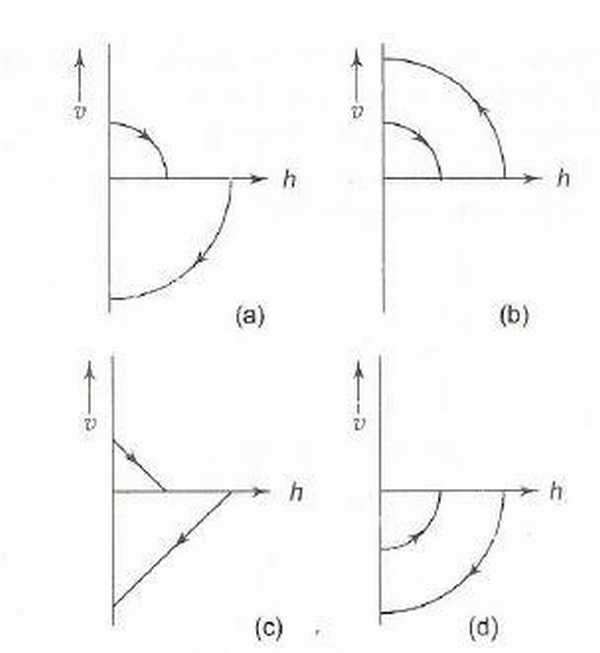
\includegraphics[scale=0.5]{Images/CC/P-Graphs/4.1e/Images/KinematicsClassicalApproach/ImagesReduced/example-previousyearsiit}%
\end{minipage}}}]~
\end{description}
\begin{quote}
\{ Hint : Case 1: Thrown from height h with zero initial velocity,
v=-gt and h = $h_{o}-1/2gt^{2}$, so eliminating t, we get $h=h_{o}-v^{2}/2g$.
So, $v=-\sqrt{2g(h_{o}-h)}$

Case 2: We assume the opposite for solving purpose that the ball is
now thrown from a height $h_{o}/2$ and replace ho only and see the
effect. Taking upward velocity as positive , we get $v=\sqrt{2g(h_{o}/2-h)}$

a) is the required answer. \}
\end{quote}

\chapter{Exercises}

\section{Review Exercise I}

\strong{Question 1.} A spark timer/air table produced the tape pictured
below. 

\doublebox{\begin{minipage}[t]{0.72\columnwidth}%
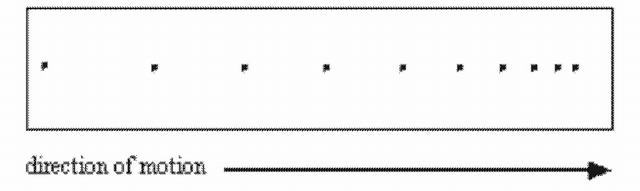
\includegraphics[scale=0.5]{Images/CC/P-Graphs/4.1e/Images/Kinematics/22}%
\end{minipage}}

The object, moving to the right, was 

a. moving with uniform motion 

b. speeding up 

c. slowing down 

d. travelling with constant speed 

\{ Hint: c\}

\strong{Question 2.} Study the position-time graph pictured below
and select the statement that is true.

\doublebox{\begin{minipage}[t]{0.72\columnwidth}%
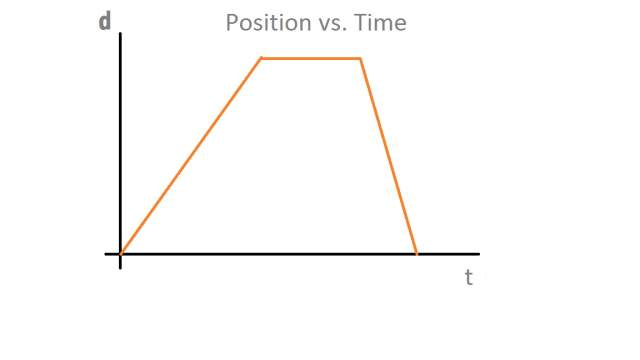
\includegraphics[scale=0.75]{Images/CC/P-Graphs/Common/Reduced/reviewkinematics/positionvstime}%
\end{minipage}}

a. The object accelerates, stops, then accelerates in the opposite
direction. 

b. The object's speed is greatest during the first segment. 

c. The object's acceleration is greatest during the last segment. 

d. The object's average velocity is zero. 

e. The object travels a greater distance in the first segment than
in the last segment.

\{ Hint : D \}

\strong{Question 3.} The position-time graph pictured below represents
the motions of two objects, A and B. Which of the following statements
concerning the objects' motions is true? 

\doublebox{\begin{minipage}[t]{0.72\columnwidth}%
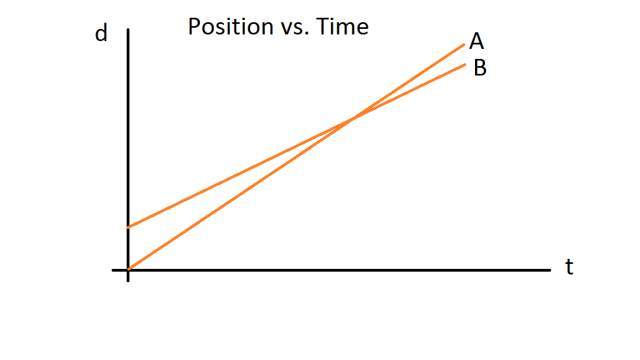
\includegraphics[scale=0.5]{Images/CC/P-Graphs/Common/Reduced/reviewkinematics/32}%
\end{minipage}}

a. Object B travels the greater distance. 

b. Object A has the greater speed. 

c. Object A leaves the reference point at an earlier time. 

d. Both objects have the same speed at the point where the lines cross. 

e. Object A is travelling for a longer period of time. 

\{ Hint : B \}

\strong{Question 4.} The position-time graph pictured below represents
a race between three contestants A, B, and C. The race begins at time
zero at the sound of the starter's pistol. Which of the following
statements is true? 

\doublebox{\begin{minipage}[t]{0.72\columnwidth}%
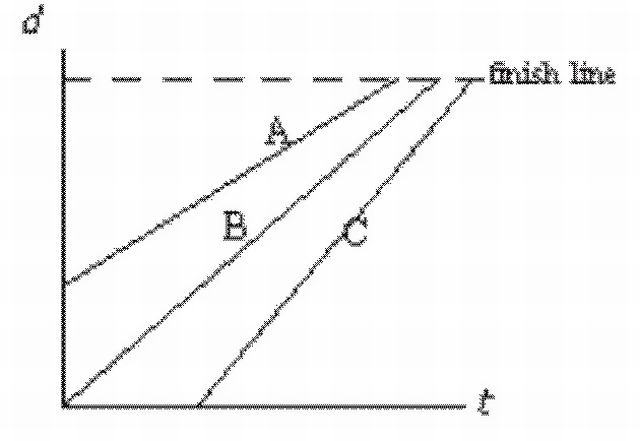
\includegraphics[scale=0.5]{Images/CC/P-Graphs/4.1e/Images/Kinematics/33}%
\end{minipage}}

a. The runner who started last finished first. 

b. The fastest runner won the race. 

c. The runner with a head start won the race. 

d. Only one runner began at the sound of the starter's pistol. 

e. All runners ran the same distance. 

\{ Hint : C \}

\strong{Question 5.} The position-time graph pictured below depicts
a person, P, running to catch a bus, B, that has just begun to pull
away. Which of the following statements is true? 

\doublebox{\begin{minipage}[t]{0.72\columnwidth}%
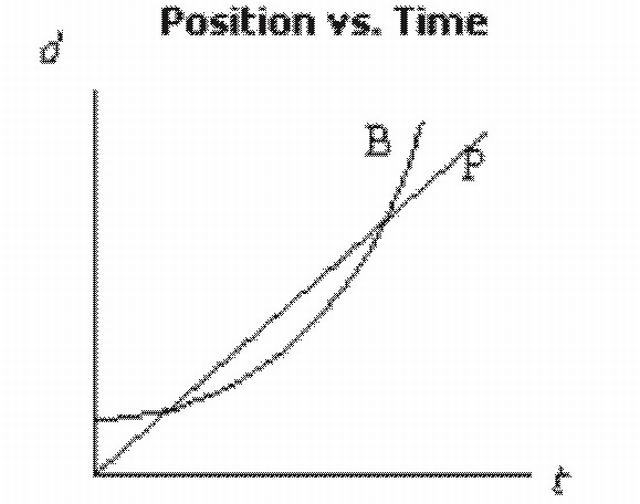
\includegraphics[scale=0.5]{Images/CC/P-Graphs/4.1e/Images/Kinematics/34}%
\end{minipage}}

a. The person has no chance of catching the bus. 

b. The person's acceleration is greater than that of the bus.

c. The person has two opportunities to catch up to the bus. 

d. The speed of the bus is always greater than that of the person.

e. The person's speed is always greater than that of the bus. 

\{ Hint : C\}

\strong{Question 6.} The position-time graph that depicts a ball
thrown vertically upward that returns to the same position is

\doublebox{\begin{minipage}[t]{0.7\columnwidth}%
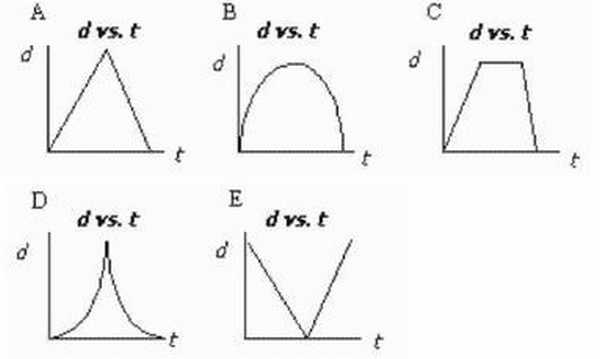
\includegraphics[scale=0.5]{Images/CC/P-Graphs/Common/Reduced/reviewkinematics/ImagesReduced/35}%
\end{minipage}}

a.A 

b. B 

c. C

d. D

e. E 

\{ Hint : B \}

\strong{Question 7.} The position-time graph that represents \textquotedbl uniform
motion\textquotedbl{} is 

\doublebox{\begin{minipage}[t]{0.72\columnwidth}%
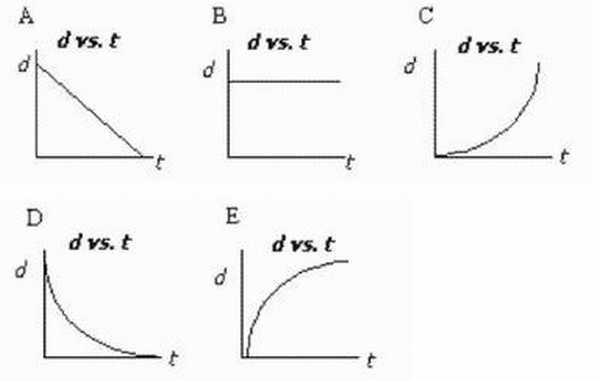
\includegraphics[scale=0.5]{Images/CC/P-Graphs/Common/Reduced/reviewkinematics/ImagesReduced/36}%
\end{minipage}}

a. A 

b. B 

c. C 

d. D 

e. E 

\{ Hint : A\}

\strong{Question 8.} The velocity-time graph that represents \textquotedbl uniform
motion\textquotedbl{} is 

\doublebox{\begin{minipage}[t]{0.72\columnwidth}%
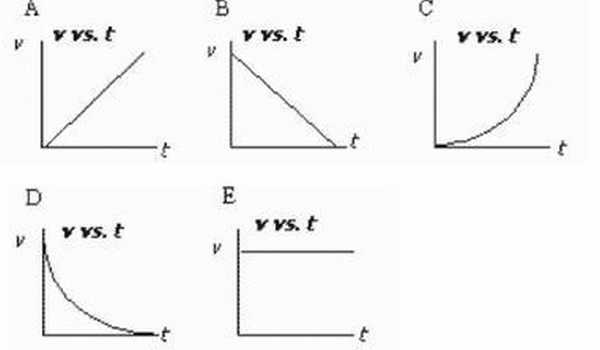
\includegraphics[scale=0.5]{Images/CC/P-Graphs/Common/Reduced/reviewkinematics/ImagesReduced/37}%
\end{minipage}}

a. A 

b. B 

c. C

d. D 

e. E

\{ Hint : E \}

\strong{Question 9.} The velocity-time graph pictured below depicts
the motion of a motorcycle. Which of the following statements is true? 

\doublebox{\begin{minipage}[t]{0.72\columnwidth}%
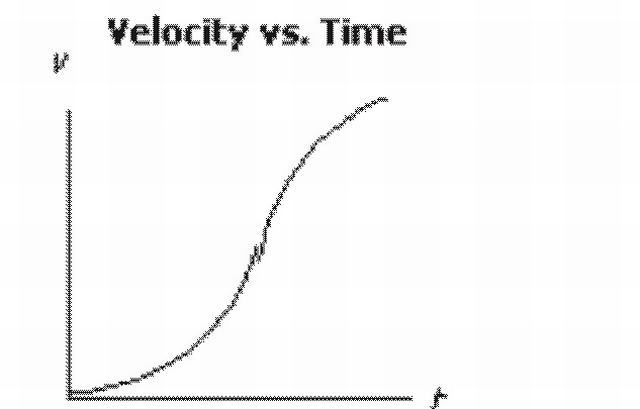
\includegraphics[scale=0.5]{Images/CC/P-Graphs/4.1e/Images/Kinematics/38}%
\end{minipage}}

a. The motorcycle is always experiencing an acceleration. 

b. The motorcycle's greatest speed occurs toward the end of the recorded
time interval. 

c. The motorcycle's average acceleration is zero.

d. The motorcycle eventually reaches uniform motion. 

e. The motorcycle accelerates until it reaches a constant speed. 

\{ Hint : A \}

\strong{Question 10.} The velocity-time graph pictured below represents
the motion of a police car, P, in pursuit of a motorcycle, M. The
motorcycle has just passed the police car. Which of the following
statements is true? 

\doublebox{\begin{minipage}[t]{0.72\columnwidth}%
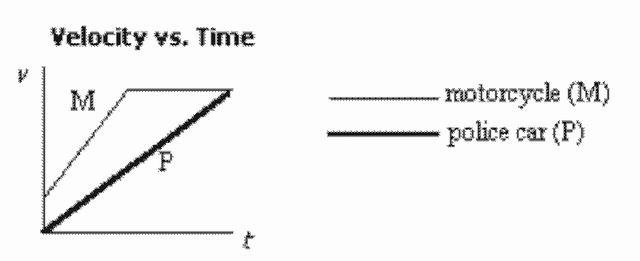
\includegraphics[scale=0.5]{Images/CC/P-Graphs/4.1e/Images/Kinematics/39}%
\end{minipage}}

a. Both vehicles are at rest when the pursuit begins. 

b. The police car eventually catches the motorcycle.

c. The motorcycle accelerates and then slows down. 

d. At the end of the recorded time interval, the police car has yet
to catch the motorcycle. 

e. The police car passes the motorcycle. 

\{ Hint : D \}

\strong{Question 11.} Consider the following velocity-time graph
and select the statement that is true. 

\doublebox{\begin{minipage}[t]{0.72\columnwidth}%
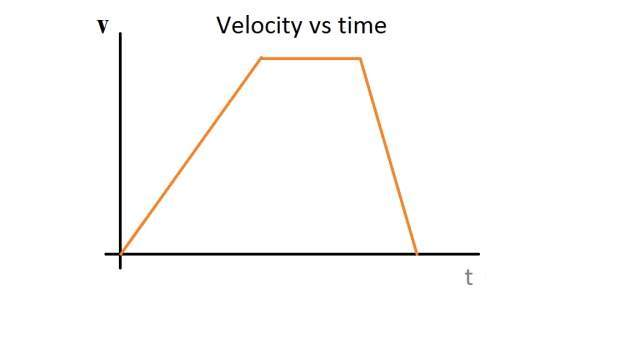
\includegraphics[scale=0.75]{Images/CC/P-Graphs/Common/Reduced/reviewkinematics/velocityvstime}%
\end{minipage}}

a. At no time can the motion be considered \textquotedbl uniform.\textquotedbl{} 

b. The object returns to its original position. 

c. The object travels in one direction and then the other. 

d. The object is accelerating throughout the entire recorded time. 

e. The object speeds up and later slows down. 

\{ Hint : E \}

\_\_\_\_ 41. Which of the following velocity-time graphs represents
the motion of a ball thrown vertically upward? 

\doublebox{\begin{minipage}[t]{0.72\columnwidth}%
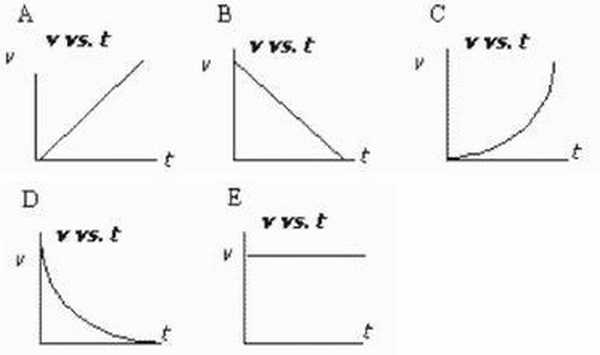
\includegraphics[scale=0.5]{Images/CC/P-Graphs/Common/Reduced/reviewkinematics/ImagesReduced/41}%
\end{minipage}}

a. A

b. B

c. C

d. D

e. E

\{ Hint : B \}

\_\_\_\_ 42. The following velocity-time graph depicts the motions
of two objects, A and B. Which of the statements describing the graph
is true?

\doublebox{\begin{minipage}[t]{0.72\columnwidth}%
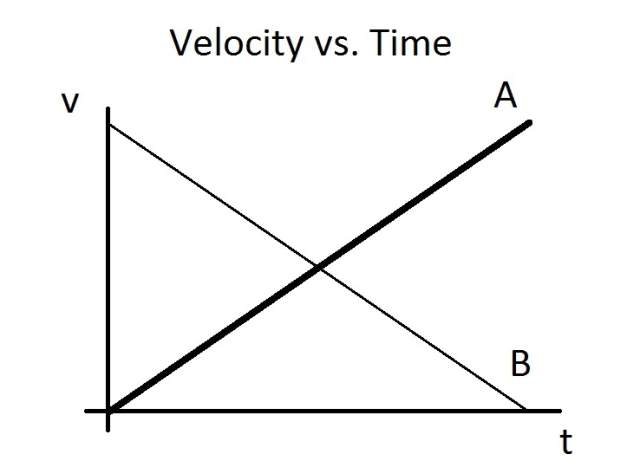
\includegraphics[scale=0.75]{Images/CC/P-Graphs/Common/Reduced/reviewkinematics/42}%
\end{minipage}}

a. Both objects are accelerating uniformly. 

b. The two objects are travelling in opposite directions.

c. Both objects start from rest. 

d. Object A travels farther than object B.

e. Object B travels farther than object A. 

\{ Hint : A \}

\_\_\_\_ 43. Which statement describes the motion represented by the
following acceleration-time graph? 

\doublebox{\begin{minipage}[t]{0.72\columnwidth}%
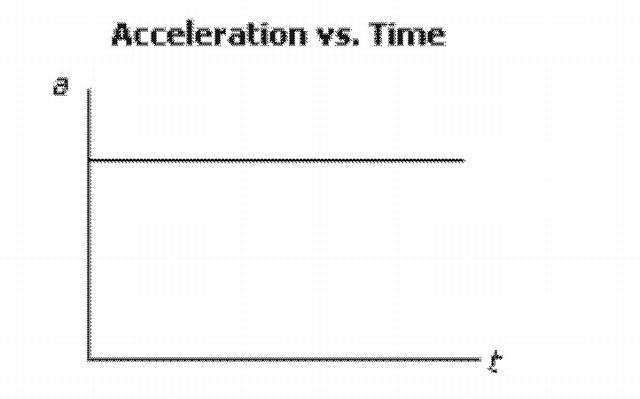
\includegraphics[scale=0.5]{Images/CC/P-Graphs/4.1e/Images/Kinematics/43}%
\end{minipage}}

a. The object is moving with uniform motion.

b. The object has a constant velocity. 

c. The object has a uniform acceleration. 

d. The object is stopped. 

e. The object has a changing acceleration. 

\{ Hint : C \}

\_\_\_\_ 44. A ball is thrown vertically upward into the air. Which
of the following acceleration-time graphs represents the ball's motion? 

\doublebox{\begin{minipage}[t]{0.72\columnwidth}%
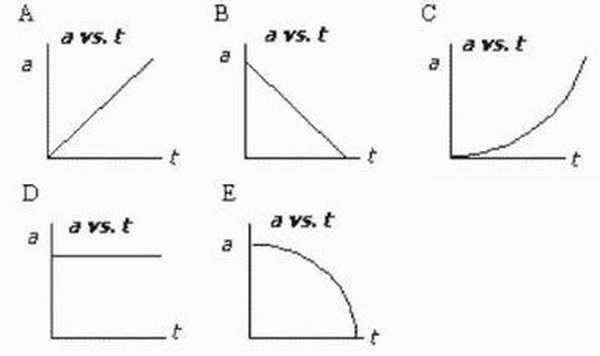
\includegraphics[scale=0.5]{Images/CC/P-Graphs/Common/Reduced/reviewkinematics/ImagesReduced/44}%
\end{minipage}}

a. A 

b. B 

c. C

d. D

e. E

\{ Hint : D \}

\_\_\_\_ 45. Four of the five graphs pictured below could all represent
the same motion. Which graph does not belong to this group? 

\doublebox{\begin{minipage}[t]{0.72\columnwidth}%
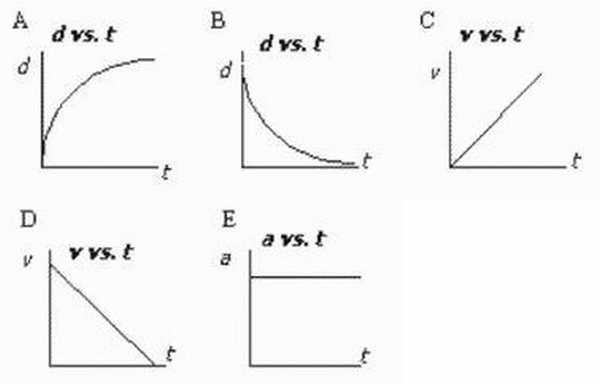
\includegraphics[scale=0.5]{Images/CC/P-Graphs/Common/Reduced/reviewkinematics/ImagesReduced/45}%
\end{minipage}}

a. A 

b. B 

c. C

d. D

e. E

\{ Hint : C \}

\_\_\_\_ 49. The position-time graph below depicts the motions of
two objects, A and B. Which of the following statements concerning
the objects' motions is NOT true? 

\doublebox{\begin{minipage}[t]{0.72\columnwidth}%
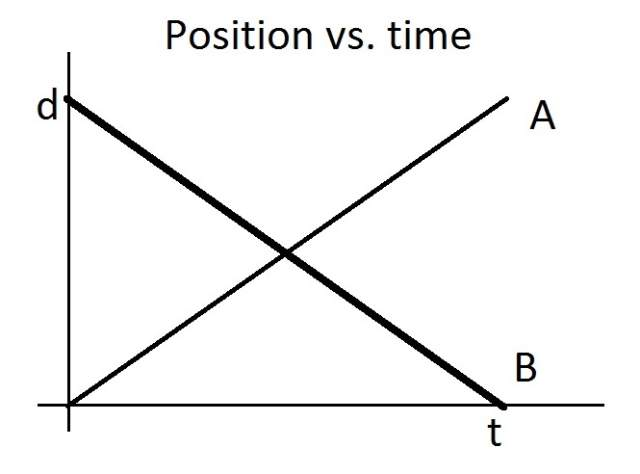
\includegraphics[scale=0.5]{Images/CC/P-Graphs/Common/Reduced/reviewkinematics/49}%
\end{minipage}}

a. The two objects have the same speed.

b. The two objects travel the same distance. 

c. The two objects travel with uniform motion.

d. The two objects travel for the same amount of time. 

e. The two objects have the same velocity.

\{ Hint : E \}

\_\_\_\_ 50. What type of motion is depicted by the following acceleration-time
graph? 

\doublebox{\begin{minipage}[t]{0.72\columnwidth}%
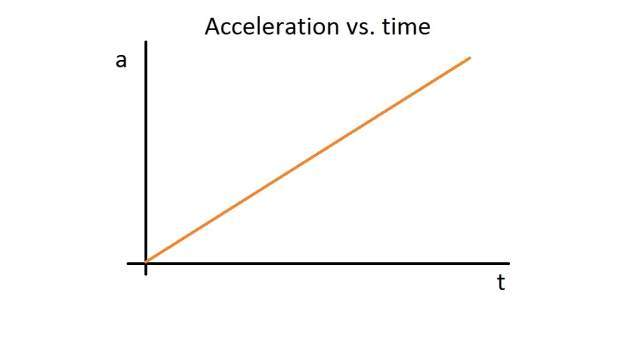
\includegraphics[scale=0.5]{Images/CC/P-Graphs/Common/Reduced/reviewkinematics/50}%
\end{minipage}}

a. constant velocity b. non-uniformly changing acceleration c. constant
acceleration d. uniformly changing acceleration e. uniform motion 

\{ Hint: D\}

\_\_\_\_ 51. The diagram below shows the first three legs of a trip:
A to B, B to C, and C to D. If a person returns from point D to point
A, what is the displacement for this fourth and final leg? 

\doublebox{\begin{minipage}[t]{0.72\columnwidth}%
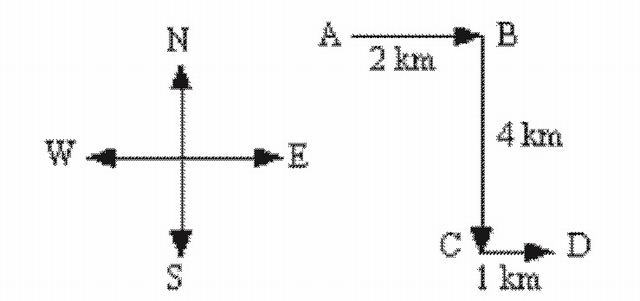
\includegraphics[scale=0.5]{Images/CC/P-Graphs/4.1e/Images/Kinematics/51}%
\end{minipage}}

a. 7 km {[}37� W of N{]} 

b. 5 km {[}37� W of N{]}

c. 5 km {[}37� E of S{]}

d. 7 km {[}37� E of S{]}

e. 5 km {[}37� N of E{]} 

\{ Hint : B \}

\section{Review Exercise II}

1. A cart travels with a constant nonzero acceleration along a straight
line. Which graph best represents the relationship between the distance
the cart travels and time of travel? 

\doublebox{\begin{minipage}[t]{0.72\columnwidth}%
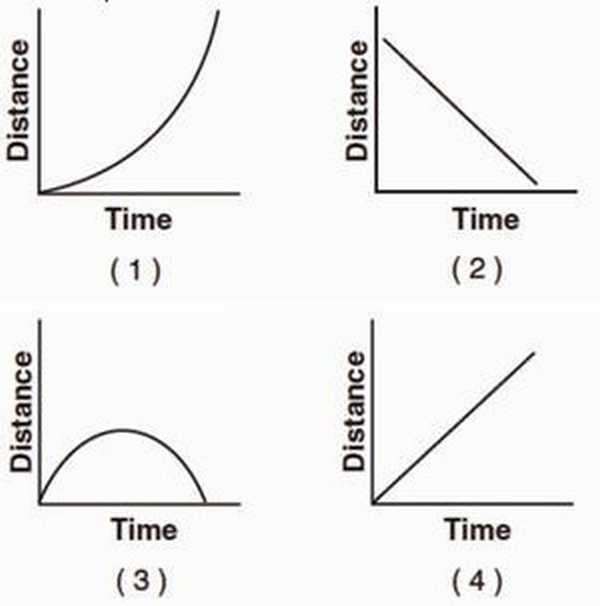
\includegraphics[scale=0.5]{Images/CC/P-Graphs/Common/Reduced/reviewkinematics/ImagesReduced/1_1_rev}%
\end{minipage}}

\{ Hint: First of all the graph should be a parabola. Secondly, it
can't be (3) as distance can only increase. \}

Base your answers to questions 2 through 4 on the information below. 

A car on a straight road starts from rest and accelerates at 1.0 meter
per second$^{2}$ for 10 seconds. Then the car continues to travel
at constant speed for an additional 20 seconds. 

2. Determine the speed of the car at the end of the first 10 seconds. 

\{ Hint : v=at, so v at 10 s = 10 m/s\}

3. On the grid at below, use a ruler or straightedge to construct
a graph of the car\textquoteright s speed as a function of time for
the entire 30-second interval. 

\doublebox{\begin{minipage}[t]{0.72\columnwidth}%
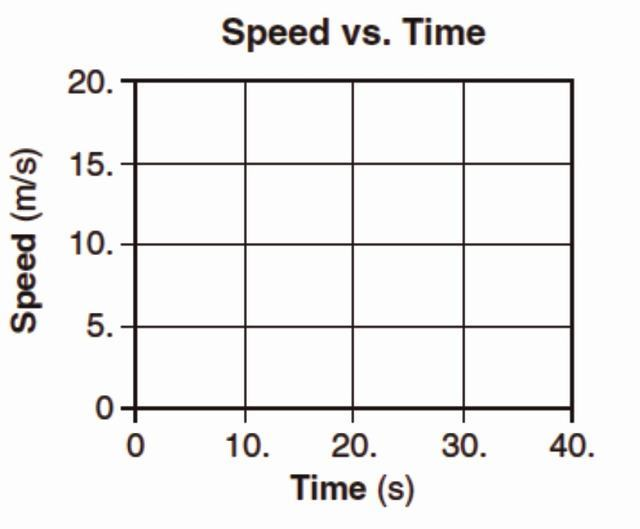
\includegraphics[scale=0.5]{Images/CC/P-Graphs/4.1e/Images/Kinematics/1_3}%
\end{minipage}}

\{ Hint: Try out yourself. \}

4. Calculate the distance the car travels in the first 10 seconds.
{[}Show all work, including the equation and substitution with units.{]} 

\{ Hint: s=$1/2at^{2}$ = 50m \}

5. A student throws a baseball vertically upward and then catches
it. If vertically upward is considered to be the positive direction,
which graph best represents the relationship between velocity and
time for the baseball? {[}Neglect friction.{]} 

\doublebox{\begin{minipage}[t]{0.72\columnwidth}%
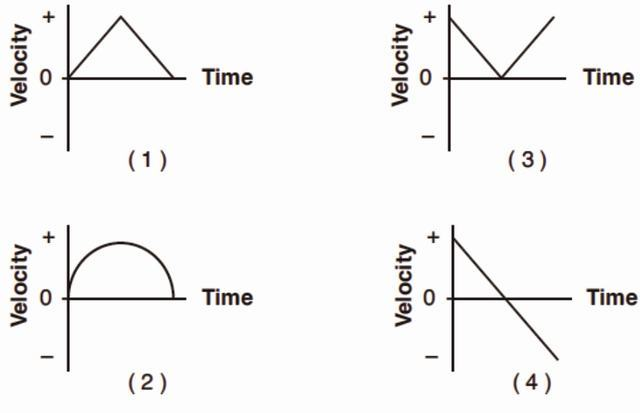
\includegraphics[scale=0.5]{Images/CC/P-Graphs/4.1e/Images/Kinematics/1_5}%
\end{minipage}}

\{ Hint : v=u-gt, so velocity is continually decreasing with 9.81
m/s and even turns negative, equal to the initial value in magnitude
on return and opposite direction if air drag is neglected. 

D) is the correct option. \}

6. The graph below represents the displacement of an object moving
in a straight line as a function of time.

\doublebox{\begin{minipage}[t]{0.72\columnwidth}%
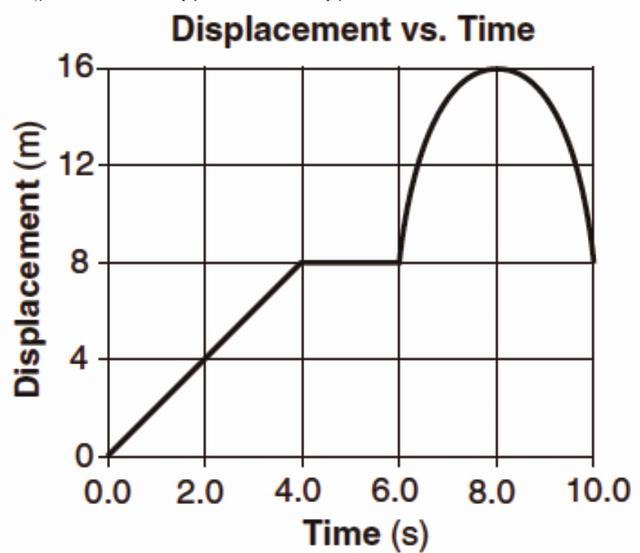
\includegraphics[scale=0.5]{Images/CC/P-Graphs/4.1e/Images/Kinematics/1_6}%
\end{minipage}}

What was the total distance traveled by the object during the 10-second
time interval? 

1. 0 m 

2. 8 m 

3. 16 m 

4. 24 m 

\{ Hint: The object moves 16m forward and 8m backward. So, distance
is 24 m.

4) is the correct option. \}

7. Which graph best represents the relationship between the acceleration
of an object falling freely near the surface of Earth and the time
that it falls? 

\doublebox{\begin{minipage}[t]{0.72\columnwidth}%
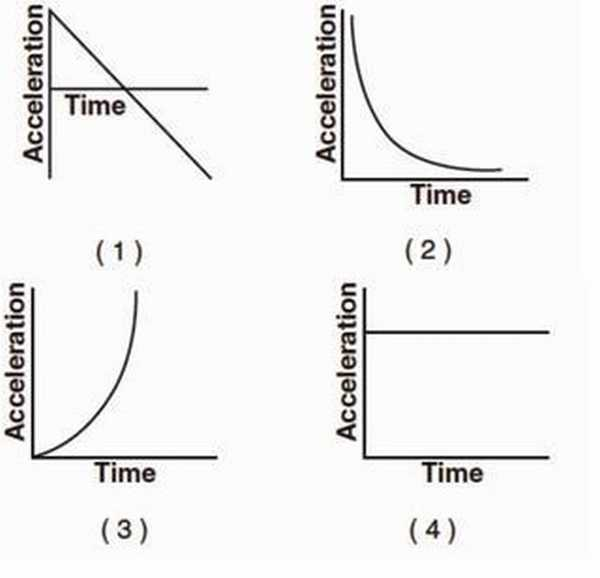
\includegraphics[scale=0.5]{Images/CC/P-Graphs/Common/Reduced/reviewkinematics/ImagesReduced/1_7_rev}%
\end{minipage}}

\{ Hint : Acceleration due to gravity near the earth surface is constant,
being 9.81 $m/s^{2}$ \}

8. Which pair of graphs represent the same motion of an object?

\doublebox{\begin{minipage}[t]{0.72\columnwidth}%
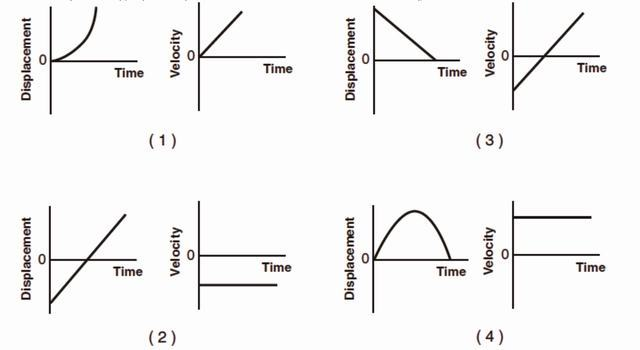
\includegraphics[scale=0.5]{Images/CC/P-Graphs/4.1e/Images/Kinematics/1_8}%
\end{minipage}}

\{ Hint : A) \}

9. The graph below represents the velocity of an object traveling
in a straight line as a function of time. 

\doublebox{\begin{minipage}[t]{0.72\columnwidth}%
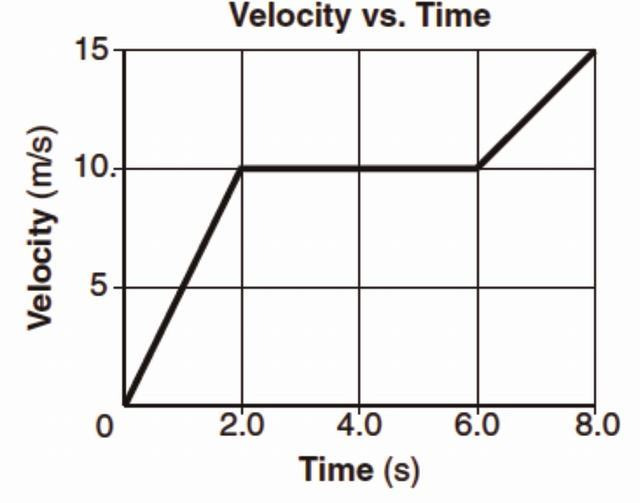
\includegraphics[scale=0.5]{Images/CC/P-Graphs/4.1e/Images/Kinematics/1_9}%
\end{minipage}}

Determine the magnitude of the total displacement of the object at
the end of the first 6 seconds. 

\{Hint 50m, area under the graph till 6s.: \}

10. Which graph best represents the motion of a block accelerating
uniformly down an inclined plane? 

\doublebox{\begin{minipage}[t]{0.72\columnwidth}%
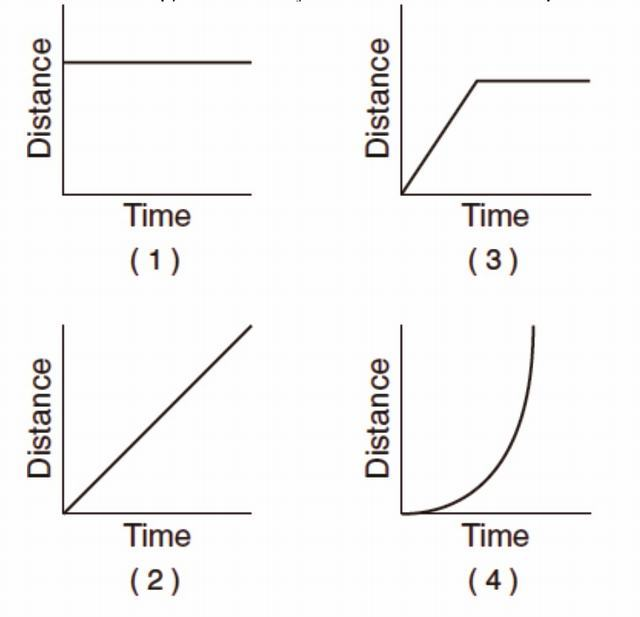
\includegraphics[scale=0.5]{Images/CC/P-Graphs/4.1e/Images/Kinematics/1_10}%
\end{minipage}}

\{Hint: (4) as the graph would be a function of $t^{2}$, calculated
via the usual equations of motion for uniformly accelerated motion.\}

Base your answers to questions 11 and 12 on the graph below, which
represents the motion of a car during a 6-second time interval. 

\doublebox{\begin{minipage}[t]{0.72\columnwidth}%
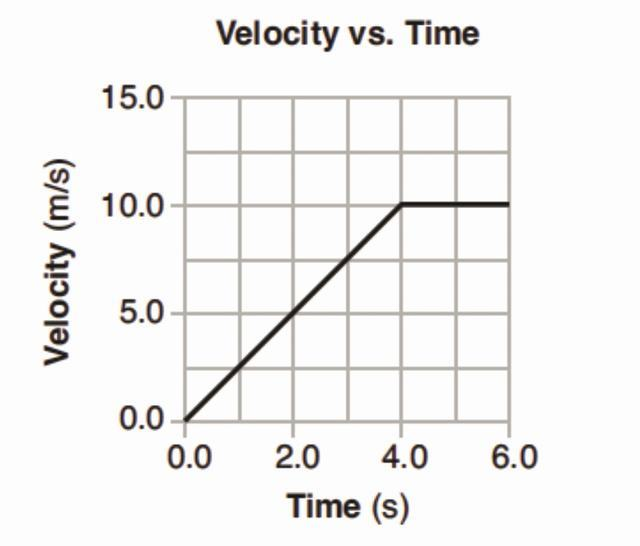
\includegraphics[scale=0.5]{Images/CC/P-Graphs/4.1e/Images/Kinematics/1_11plus12}%
\end{minipage}}

11. What is the acceleration of the car at t=5.0 seconds? 

1. 0.0 m/s2 

2. 2.0 m/s2 

3. 2.5 m/s2 

4. 10 m/s2 

\{Hint : It is the slope of v-t graph, at t=5.0, the graph has zero
slope. So, (1)\}

12. What is the total distance traveled by the car during this 6-second
interval?

1. 10 m 

2. 20 m 

3. 40 m 

4. 60 m 

\{ Hint : Area under the v-t curve, 40m, So, (3)\}

13. Which graph best represents the relationship between the velocity
of an object thrown straight upward from Earth\textquoteright s surface
and the time that elapses while it is in the air? {[}Neglect friction.{]} 

\doublebox{\begin{minipage}[t]{0.72\columnwidth}%
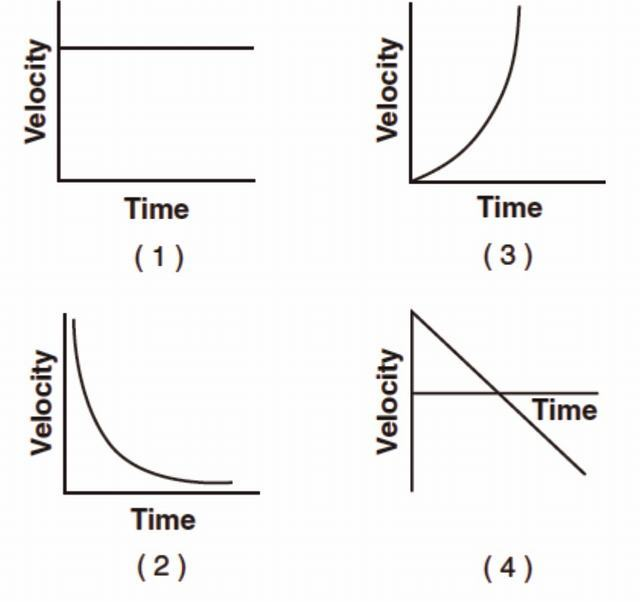
\includegraphics[scale=0.5]{Images/CC/P-Graphs/4.1e/Images/Kinematics/1_13}%
\end{minipage}}

\{ Hint : (4) \}

14. The graph below shows the relationship between the speed and elapsed
time for an object falling freely from rest near the surface of a
planet. 

\doublebox{\begin{minipage}[t]{0.72\columnwidth}%
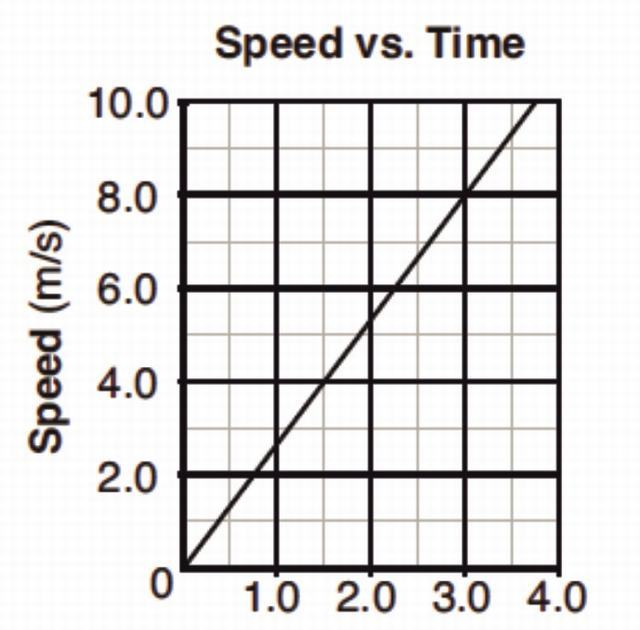
\includegraphics[scale=0.5]{Images/CC/P-Graphs/4.1e/Images/Kinematics/1_14}%
\end{minipage}}

What is the total distance the object falls during the first 3 seconds? 

1. 12 m 

2. 24 m 

3. 44 m 

4. 72 m 

\{ Hint : Area under the graph between 0 and 3, 12m\}

15. The graph below represents the relationship between speed and
time for an object moving along a straight line. 

\doublebox{\begin{minipage}[t]{0.72\columnwidth}%
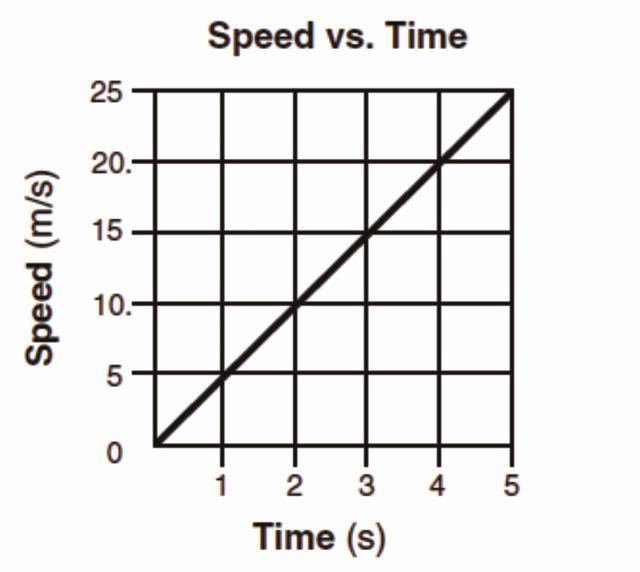
\includegraphics[scale=0.5]{Images/CC/P-Graphs/4.1e/Images/Kinematics/1_15}%
\end{minipage}}

What is the total distance traveled by the object during the first
4 seconds?

1. 5 m 

2. 20 m 

3. 40 m 

4. 80 m 

\{ Hint : 40m , So, 3\}

Base your answers to questions 16 and 17 on the graph below, which
shows the relationship between speed and elapsed time for a car moving
in a straight line. 

\doublebox{\begin{minipage}[t]{0.72\columnwidth}%
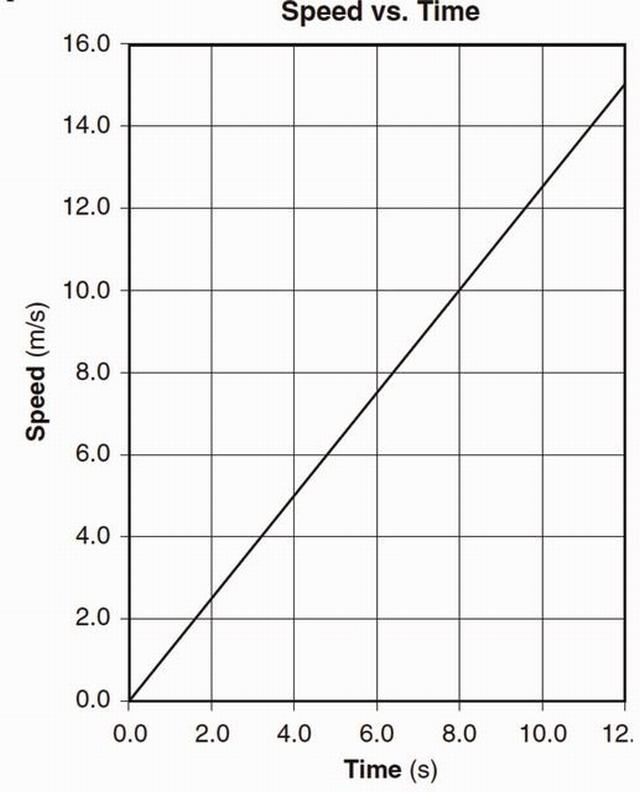
\includegraphics[scale=0.5]{Images/CC/P-Graphs/4.1e/Images/Kinematics/1_16plus17}%
\end{minipage}}

16. Determine the magnitude of the acceleration of the car. 

\{ Hint : Slope of the line , 1.25m/s2 \}

17. Calculate the total distance the car traveled during the time
interval 4.0 seconds to 8.0 seconds. {[}Show all work, including the
equation and substitution with units.{]}

\{ Hint : It's the area of trapezium with parallel sides , 5 and 10
and distance between them as 4 , = 30m \}

Base your answers to questions 18 through 20 on the graph below, which
represents the relationship between velocity and time for a car moving
along a straight line, and your knowledge of physics. 

\doublebox{\begin{minipage}[t]{0.72\columnwidth}%
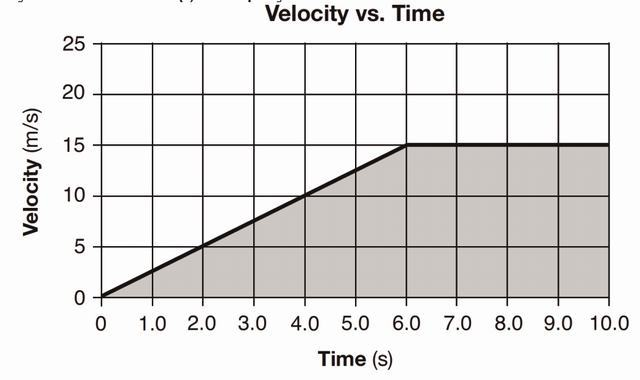
\includegraphics[scale=0.5]{Images/CC/P-Graphs/4.1e/Images/Kinematics/1_18to20}%
\end{minipage}}

18. Determine the magnitude of the average velocity of the car from
t=6.0 seconds to t=10.0 seconds. 

\{ Hint : Velocity is constant between 6 and 10 , ie 15 m/s\}

19. Determine the magnitude of the car\textquoteright s acceleration
during the first 6.0 seconds. 

\{ Hint : Slope of the graph is 1.5 m/s2\}

20. Identify the physical quantity represented by the shaded area
on the graph.

\{ Hint : Dispacement of the car from initial position by t=10.0s
, calculated to be 105m\}

\begin{comment}
\begin{btSect}[plain]{Bibliography/CC/P-Graphs/4e/kinematics}
\btPrintCited
\end{btSect}
\end{comment}

\printbibliography

\part{\index{Laws of Motion}Laws of Motion}

\chapter{Abstract Introduction}

\section{Force \textendash{} Time Graphs}

\doublebox{\begin{minipage}[t]{0.72\columnwidth}%
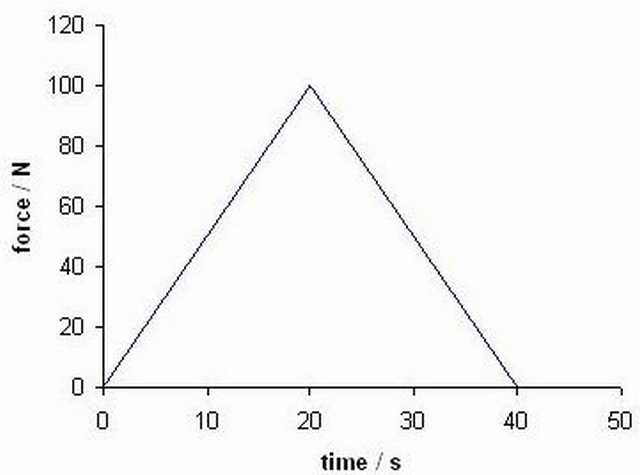
\includegraphics[scale=0.5]{Images/CC/P-Graphs/4.1e/Images/LawsOfMotion/force-time-graph1}%
\end{minipage}}

The area under a force \textendash{} time graph gives us the impulse
of the force applied (and hence the change in momentum of the object).
For this graph the impulse (the area under the graph) is 2000 kg ms$^{-1}$.\cite{physicsnet.co.uk}

\section{Change in Momentum or the \textquotedbl Impulse\textquotedbl{} }

The change in the momentum of a system (or the impulse delivered by
the net force) is given mathematically by the Momentum Principle, 

$\triangle\overrightarrow{p}=\overrightarrow{F_{net}}\triangle t$\cite{pa.msu.edu}

In this form, the change in momentum is calculated over a \textquotedblleft discrete\textquotedblright{}
time step. That is, the calculation is done over a known or determined
time interval. If the force is non-constant (i.e., depends on location
or velocity), this calculation is not exact. In fact, in this case,
the net force is the average net force over the time interval. So
that a better definition is this:

$\triangle\overrightarrow{p}=\overrightarrow{F_{net,avg}}\triangle t$

This definition works well for case where you might use iterative
procedures to determine the change in momentum over small time intervals.
If on the other hand, you can analytically integrate the force (e.g.,
it is or can be put into a form which is time dependent), then you
can use the derivative form of the Momentum Principle,

$\Delta\overrightarrow{p}=\intop_{t_{i}}^{t_{f}}\overset{\rightarrow}{F}_{net}dt$

In any event, either (or both) can be useful to think about graphs
of force vs time.

\subsection{Force vs Time Graphs }

In some situations, it is easier to empirically measure force versus
time graphs because the situations lend themselves more easily to
these empirical measurements rather than what might be more complex
physical theories. This is true in different engineering contexts
(e.g., impact design and the flow of fluids). In these cases, you
are interested in determining the change in momentum (and thus the
velocity) of the system in question1).

Below is a force vs time graph where the \textquotedblleft area under
the curve\textquotedblright{} has been highlighted. In this example,
we are only looking at the component of the net force in the xx-direction.
Such graphs can be produced for each component of the net force, but
let's say that for this system, there was a non-zero component of
the net force only in the x-direction.

\doublebox{\begin{minipage}[t]{0.72\columnwidth}%
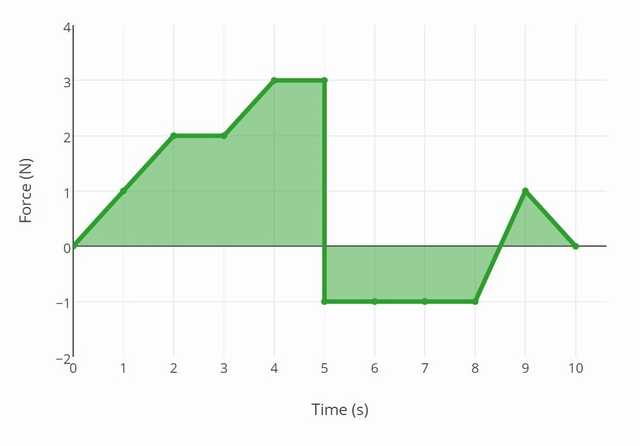
\includegraphics[scale=0.5]{Images/CC/P-Graphs/4.1e/Images/LawsOfMotion/th2}%
\end{minipage}}

For the above figure, the momentum change over the complete time interval
can be determined in a straightforward way due to the simple geometric
shapes produced. Area above the zero line are positive momentum changes,
and area below are negative. By adding up the \textquotedblleft area
under the curve\textquotedblright{} in this way, we obtain a momentum
change of 7 Ns.

The figure below shows the force vs time graph for another system.
In this case, the graph has a smooth form, which doesn't appear to
be analytic. The \textquotedblleft area under the curve\textquotedblright{}
for this graph could be analyzed computationally, by taking small
steps (i.e., Riemann Sum), and the change in momentum could be determined.

\doublebox{\begin{minipage}[t]{0.72\columnwidth}%
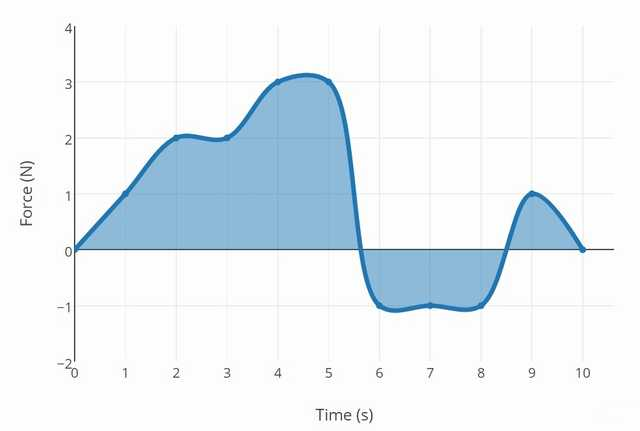
\includegraphics[scale=0.5]{Images/CC/P-Graphs/4.1e/Images/LawsOfMotion/th3}%
\end{minipage}}

1) It is possible to determine the displacement of such systems as
well. This can be done using velocity vs time graphs that are produced
from the analysis of force vs time graphs.

\section{Impulse graphs ( A Case Study) \cite{bbc.co.uk}}

The force on the squash ball in the previous question is an average
force and often the force changes during the collision. For this example
the force\textendash time graph could look like this.

\doublebox{\begin{minipage}[t]{0.72\columnwidth}%
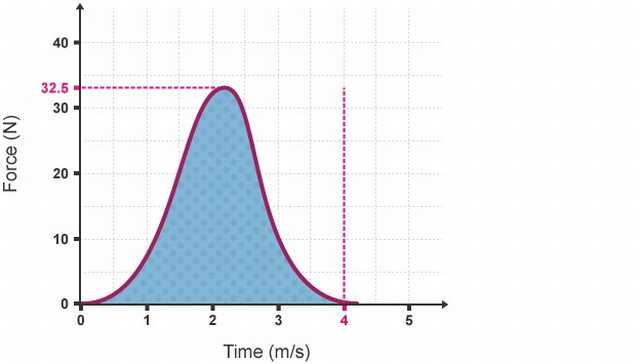
\includegraphics[scale=0.5]{Images/CC/P-Graphs/4.1e/Images/LawsOfMotion/large}%
\end{minipage}}

Notice the peak force is greater than the average force calculated. 

The area under a force time graph is equal to the impulse. For any
collision with a fixed change in momentum, if the time of contact
can be increased, the peak force is reduced:

For example if the squash ball was replaced with a softer version
of same mass the collision graph would look like this:

\doublebox{\begin{minipage}[t]{0.72\columnwidth}%
\includegraphics[scale=0.5]{\string"Images/CC/P-Graphs/4.1e/Images/LawsOfMotion/large (1)\string".jpg}%
\end{minipage}}

If the squash ball was replaced with a harder version of same mass
the collision graph would look like this:

\doublebox{\begin{minipage}[t]{0.72\columnwidth}%
\includegraphics[scale=0.5]{\string"Images/CC/P-Graphs/4.1e/Images/LawsOfMotion/large (2)\string".jpg}%
\end{minipage}}

Question Modern cars are designed to crumple on impact in a collision.
How does this help to protect the occupants from harm? 

Answer The change in momentum (area under the force time graph) can't
be changed at the time of the accident (mass is fixed and it is too
late for the driver to slow down!) By increasing the time of collision
the peak force is less and hopefully lets the occupants come to less
harm as a result.

\strong{Question} : How do I find \textquotedbl Velocity\textquotedbl{}
from \textquotedbl Force vs. Time\textquotedbl{} graph? 

\strong{Solution} : You need two additional pieces of information:
the mass of the object and its initial velocity. Given those, the
relation is:

$v(t)=v_{o}+\dfrac{1}{m}\int_{0}^{t}F(t)dt$

\chapter{\index{Friction}Friction}

\section{Static Friction \cite{hyperphysics.phy-astr.gsu.edu}}

Static frictional forces from the interlocking of the irregularities
of two surfaces will increase to prevent any relative motion up until
some limit where motion occurs. It is that threshold of motion which
is characterized by the coefficient of static friction. The coefficient
of static friction is typically larger than the coefficient of kinetic
friction.

\doublebox{\begin{minipage}[t]{0.7\columnwidth}%
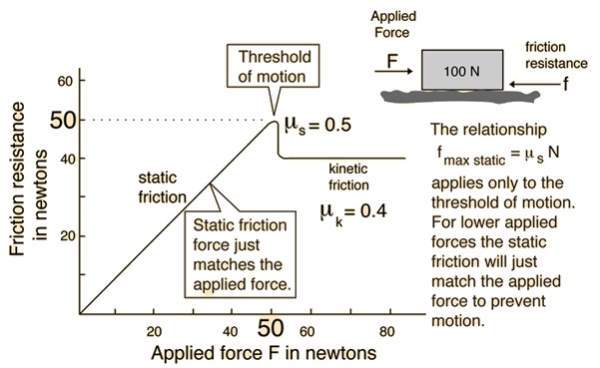
\includegraphics[scale=0.5]{Images/CC/P-Graphs/4.1e/Images/Friction/ImagesReduced/fsta}%
\end{minipage}}

In making a distinction between static and kinetic coefficients of
friction, we are dealing with an aspect of \textquotedbl real world\textquotedbl{}
common experience with a phenomenon which cannot be simply characterized.
The difference between static and kinetic coefficients obtained in
simple experiments like wooden blocks sliding on wooden inclines roughly
follows the model depicted in the friction plot from which the illustration
above is taken. This difference may arise from irregularities, surface
contaminants, etc. which defy precise description. When such experiments
are carried out with smooth metal blocks which are carefully cleaned,
the difference between static and kinetic coefficients tends to disappear.
When coefficients of friction are quoted for specific surface combinations
are quoted, it is the kinetic coefficient which is generally quoted
since it is the more reliable number.

\section{Kinetic Friction}

When two surfaces are moving with respect to one another, the frictional
resistance is almost constant over a wide range of low speeds, and
in the standard model of friction the frictional force is described
by the relationship below. The coefficient is typically less than
the coefficient of static friction, reflecting the common experience
that it is easier to keep something in motion across a horizontal
surface than to start it in motion from rest.

\doublebox{\begin{minipage}[t]{0.7\columnwidth}%
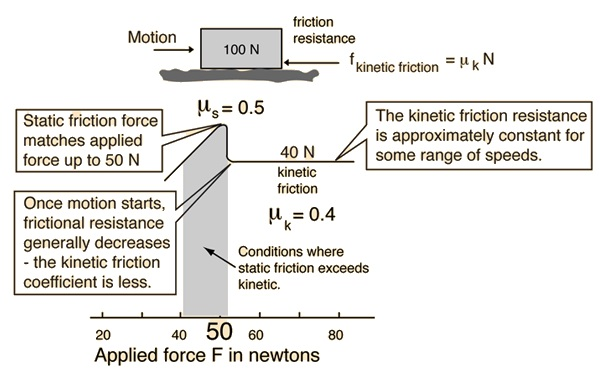
\includegraphics[scale=0.5]{Images/CC/P-Graphs/4.1e/Images/Friction/ImagesReduced/fkin}%
\end{minipage}}

\section{Friction Plot}

Static friction resistance will match the applied force up until the
threshold of motion. Then the kinetic frictional resistance stays
about constant. This plot illustrates the standard model of friction.

\doublebox{\begin{minipage}[t]{0.7\columnwidth}%
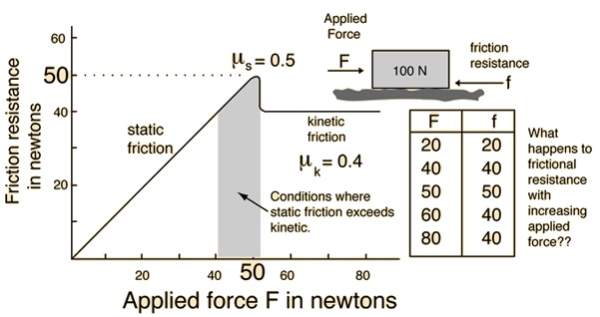
\includegraphics[scale=0.5]{Images/CC/P-Graphs/4.1e/Images/Friction/ImagesReduced/frict1}%
\end{minipage}}

The above plot, though representing a simplistic view of friction,
agrees fairly well with the results of simple experiments with wooden
blocks on wooden inclines. The experimental procedure described below
equates the vector component of the weight down the incline to the
coefficient of friction times the normal force produced by the weight
on the incline.

\doublebox{\begin{minipage}[t]{0.7\columnwidth}%
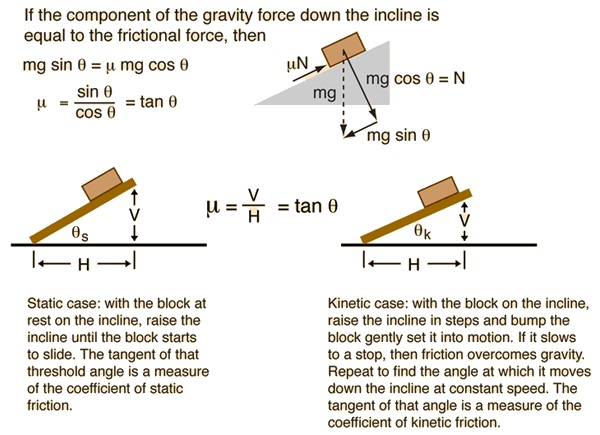
\includegraphics[scale=0.5]{Images/CC/P-Graphs/4.1e/Images/Friction/ImagesReduced/frictcoef}%
\end{minipage}}

Having taken a large number of students through this experiment, I
can report that the coefficient of static friction obtained is almost
always greater than the coefficient of kinetic friction. Typical results
for the woods I have used are 0.4 for the static coefficient and 0.3
for the kinetic coefficient.

When carefully standardized surfaces are used to measure the friction
coefficients, the difference between static and kinetic coefficients
tends to disappear, indicating that the difference may have to do
with irregular surfaces, impurities, or other factors which can be
frustratingly non-reproducible. To quote a view counter to the above
model of friction: \textquotedbl Many people believe that the friction
to be overcome to get something started (static friction) exceeds
the force required to keep it sliding (sliding friction), but with
dry metals it is very hard to show any difference. The opinion probably
arises from experiences where small bits of oil or lubricant are present,
or where blocks, for example, are supported by springs or other flexible
supports so that they appear to bind.\textquotedbl{} R. P. Feynman,
R. P. Leighton, and M. Sands, The Feynman Lectures on Physics, Vol.
I, p. 12-5, Addison-Wesley, 1964.

\section{Rolling Friction}

A rolling wheel requires a certain amount of friction so that the
point of contact of the wheel with the surface will not slip. The
amount of traction which can be obtained for an auto tire is determined
by the coefficient of static friction between the tire and the road.
If the wheel is locked and sliding, the force of friction is determined
by the coefficient of kinetic friction and is usually significantly
less.

Assuming that a wheel is rolling without slipping, the surface friction
does no work against the motion of the wheel and no energy is lost
at that point. However, there is some loss of energy and some deceleration
from friction for any real wheel, and this is sometimes referred to
as rolling friction. It is partly friction at the axle and can be
partly due to flexing of the wheel which will dissipate some energy.
Figures of 0.02 to 0.06 have been reported as effective coefficients
of rolling friction for automobile tires, compared to about 0.8 for
the maximum static friction coefficient between the tire and the road.

\section{Few problems related to Friction}
\begin{description}
\item [{Example}] : A block on the horizontal table is acted upon by a
force F. The graph of frictional force against F is
\item [{%
\doublebox{\begin{minipage}[t]{0.7\columnwidth}%
\includegraphics[scale=0.5]{\string"Images/CC/P-Graphs/4.1e/Images/LawsOfMotion/ImagesReduced/Scan_20170409 (5)\string".jpg}%
\end{minipage}}}]~
\item [{Example:}] A block rests on a rough plane whose inclination $\theta$
to the horizontal can be varied. Which of the following graphs indicates
how the frictional force F between the block and plane varies as $\theta$
is increased ?
\item [{%
\doublebox{\begin{minipage}[t]{0.7\columnwidth}%
\includegraphics[scale=0.5]{\string"Images/CC/P-Graphs/4.1e/Images/LawsOfMotion/ImagesReduced/Scan_20170409 (5) 2\string".jpg}%
\end{minipage}}}]~
\item [{Example}] : Block A is placed on block B, whose mass is greater
than that of A.
\item [{%
\doublebox{\begin{minipage}[t]{0.7\columnwidth}%
\includegraphics[scale=0.7]{\string"Images/CC/P-Graphs/4.1e/Images/LawsOfMotion/ImagesReduced/Scan_20170418 (2)\string".jpg}%
\end{minipage}}}]~
\end{description}
There is friction between the blocks, while the ground is smooth.
A horizontal force P, increasing linearly with time, begins to act
on A. The accelerations $a_{1}$ and $a_{2}$ of A and B respectively
are plotted against time (t). Choose the correct graph.

\doublebox{\begin{minipage}[t]{0.7\columnwidth}%
\includegraphics[scale=0.5]{\string"Images/CC/P-Graphs/4.1e/Images/LawsOfMotion/ImagesReduced/Scan_20170418 (2)_trai\string".jpg}%
\end{minipage}}
\begin{description}
\item [{Example}] : A body moves with uniform speed on a rough surface.
If force F of dynamic friction is plotted with time t as shown in
figure, the graph will be
\end{description}
\doublebox{\begin{minipage}[t]{0.7\columnwidth}%
\includegraphics[scale=0.5]{\string"Images/CC/P-Graphs/4.1e/Images/LawsOfMotion/ImagesReduced/Scan_20170409 (4)\string".jpg}%
\end{minipage}}

\chapter{Theory and Problems}

\section{Impulse as Force-time Graph}

\strong{Example} : For the graph shown above, assume that it shows
a constant force of 25 N acting over a 10 s period of time. Determine
the impulse. 

\doublebox{\begin{minipage}[t]{0.72\columnwidth}%
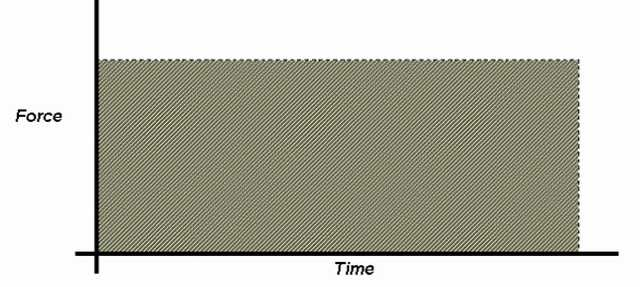
\includegraphics[scale=0.5]{Images/CC/P-Graphs/4.1e/Images/LawsOfMotion/im1}

Illustration : Graph of Example (Force as a function of Time)%
\end{minipage}}

\strong{Solution} : (Theory : So far we've implied some things about
what is constant and what can change in the impulse formula F \textgreek{D}t
= m \textgreek{D}v. 

We look at situations where we expect the mass of the object will
stay constant. \textbullet{} The velocity will change, and that's
why we put a delta in front of it. \textbullet{} Time is changing
(sort of) as we measure it over a period of time. \textbullet{} Force
must be a constant. We assume that the force being exerted on the
object was always the same, causing a constant acceleration. If we
are looking at a simple impulse question (where the force is constant),
we can figure out exactly what we can interpret from a graph. \textbullet{}
Later this may help us to figure out a more complicated question,
like if the force changes. The following graph is an example of one
of those simple situations where the force remains constant during
the entire time. \textbullet{} If we look at what the slope might
represent, we get... 

slope = rise / run 

slope = F / $\triangle$t 

Since nothing in the impulse formula can be rearranged to give us
force over time, the slope doesn't mean anything to us in this situation.

If we look at the area under the line, we get something a bit better...

Area = lw = F$\triangle$t = $\triangle$p )

Since area under the line is equal to impulse... 

Area = lw 

Area = 25$\times$10 

Area = 2.5e2 

p = 2.5e2Ns 

If we really wanted to, we could have simply use \textgreek{D}p =
F\textgreek{D}t to figure out the impulse. We could do this in this
situation because the force is constant. \textbullet{} If we need
to do a question where the force is not constant, we can still use
the area under the line to get the impulse, even though the formula
\textgreek{D}p = F\textgreek{D}t can not be used. 

\strong{Example} : I am in a car that is accelerating from rest at
a red light. I want to calculate the impulse that is acting on the
car during the first 5.78s. If I know that the force on the car steadily
increases from 0 N to 3012 N over this time, determine the impulse.
If the mass of the car is 1500 kg, also determine the final velocity
of the car. 

\doublebox{\begin{minipage}[t]{0.72\columnwidth}%
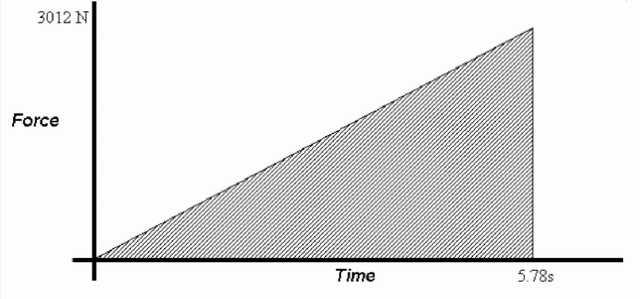
\includegraphics[scale=0.5]{Images/CC/P-Graphs/4.1e/Images/LawsOfMotion/im2}

Illustration : Graph for Example (Force as a function of Time)%
\end{minipage}}

\strong{Solution} : Let\textquoteright s start by graphing the information
we were given. We will get a nice linear graph, since it said that
the force steadily increases. 

If we calculate the area under the graph (a triangle) we will know
what the impulse is. 

A = \textonehalf{} bh 

= \textonehalf{} (5.78 s)(3012 N) 

= 8704.68 A 

= 8.70e3 kgm/s

To calculate the final velocity, we can use the value for the impulse
we just got with the right hand side of the impulse formula. Remember
that the initial velocity (sitting at the light) is zero... 

\textgreek{D} p=m\textgreek{D}v 

\textgreek{D} p=m(v$_{f}$\textminus v$_{i}$) 

\textgreek{D} p=mv$_{f}$

v$_{f}$=\textgreek{D} p m 

v$_{f}$=8704.68/1500 

v$_{f}$=5.80312 

v$_{f}$=5.80m/s 

The graph that we make does not have to be a pretty right angle triangle
either. We can also do some crazy stuff with what we are looking for
in the question, as the next example shows. 

\strong{Example} : This graph shows the result of applying 500 kgm/s
of impulse to an object as it moved across the floor for 10.0 s. Determine
the maximum force that was exerted. 

\doublebox{\begin{minipage}[t]{0.72\columnwidth}%
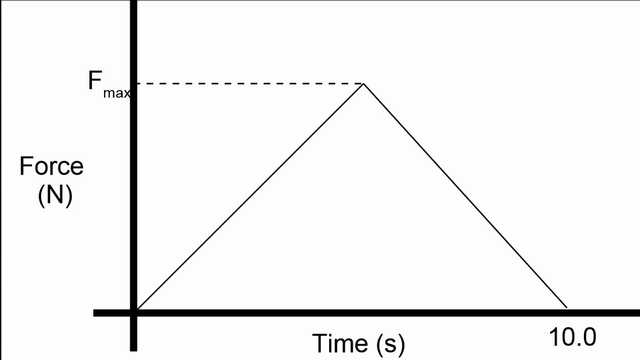
\includegraphics[scale=0.5]{Images/CC/P-Graphs/4.1e/Images/LawsOfMotion/im3}

Illustration 3: Pushing object across the floor.%
\end{minipage}}

\strong{Solution} : Even though it is not a right angle triangle,
this graph still shows a triangle that we can use the regular area
formula with. In this case, we already know the area (the impulse
is 500 kgm/s) and we know the base (10.0 s). All we want is the height
of the triangle, since that is the magnitude of the maximum force. 

Area=bh/2

$\triangle$p=F$\triangle$t/2 

F=2 $\triangle$p/ t = 2$\times$500/10.0 F=100N

Even if the graph is a curved line, you can still at least estimate
the area under the graph. \textbullet{} Although this will only be
an approximate area, without getting into calculus it's as good as
you'll get and as good as you need. \textopenbullet{} On the graph
shown below we have an s-curve that would be difficult to calculate
the exact area of. \textopenbullet{} Instead, we just look at the
triangle drawn in red. For the little bit extra it has near the beginning,
it misses a bit later on. These two parts should more or less make
up for each other, so that the area of the triangle will be about
the same as the area under the curve. 

\doublebox{\begin{minipage}[t]{0.72\columnwidth}%
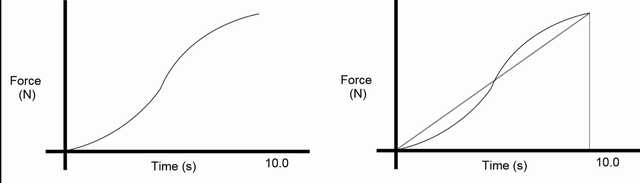
\includegraphics[scale=0.5]{Images/CC/P-Graphs/4.1e/Images/LawsOfMotion/im4}

Illustration 4: Instead of trying to figure out the area of the curve
exactly, we just use the area of the triangle as an approximation.%
\end{minipage}}

\section{Force Time graph with respect to momentum }

\doublebox{\begin{minipage}[t]{0.72\columnwidth}%
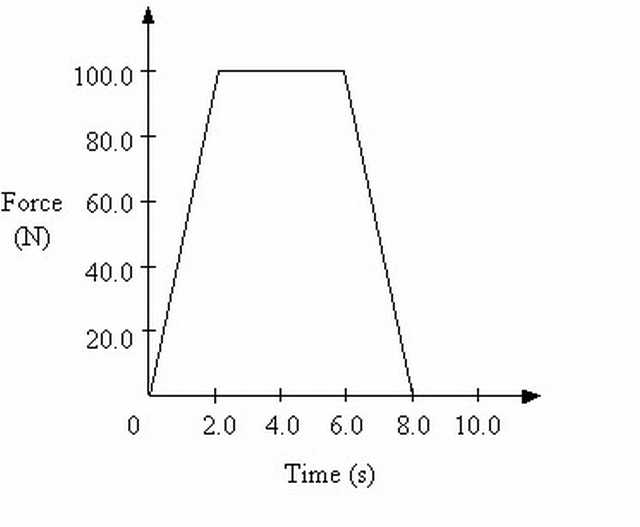
\includegraphics[scale=0.5]{Images/CC/P-Graphs/4.1e/Images/LawsOfMotion/graph}%
\end{minipage}}

\strong{Example} : If the mass of the object is 3.0 kg, what is its
final velocity over the 8.0 s time period? \cite{physicsforums.com}

\strong{Solution} : You need the area under the curve, and you do
not need calculus, as that is a trapezoid. The area of a trapezoid
is the average of the bases times the height, which is (4 + 8)seconds/2{*}100
N = 600 N{*}s. Set this to $mv-mv_{o}$, and assuming $v_{o}$ is
zero get v final = 200 m/s.

\strong{Example} : The graph given below belongs to an object having
mass 2kg and velocity 10m/s. It moves on a horizontal surface. If
a force is applied to this object between (1-7) seconds find the velocity
of the object at 7 seconds. \cite{physicstutorials.org}

\doublebox{\begin{minipage}[t]{0.72\columnwidth}%
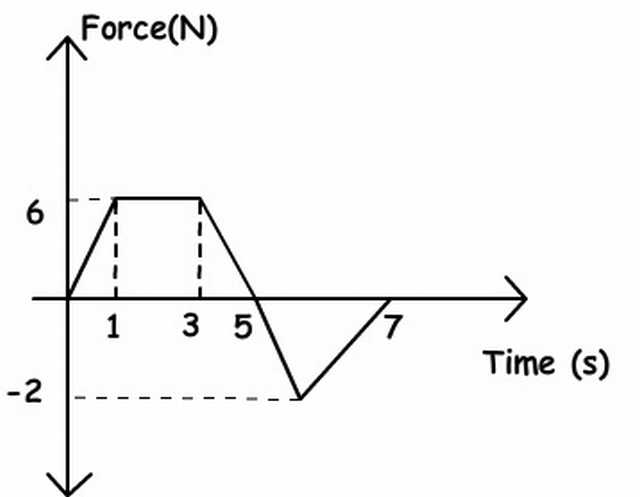
\includegraphics[scale=0.5]{Images/CC/P-Graphs/4.1e/Images/LawsOfMotion/eample46}%
\end{minipage}}

\strong{Solution} : Area under the graph gives us impulse. First,
we find the total impulse with the help of graph given above then
total impulse gives us the momentum change. Finally, we find the final
velocity of the object from the momentum change.

\doublebox{\begin{minipage}[t]{0.72\columnwidth}%
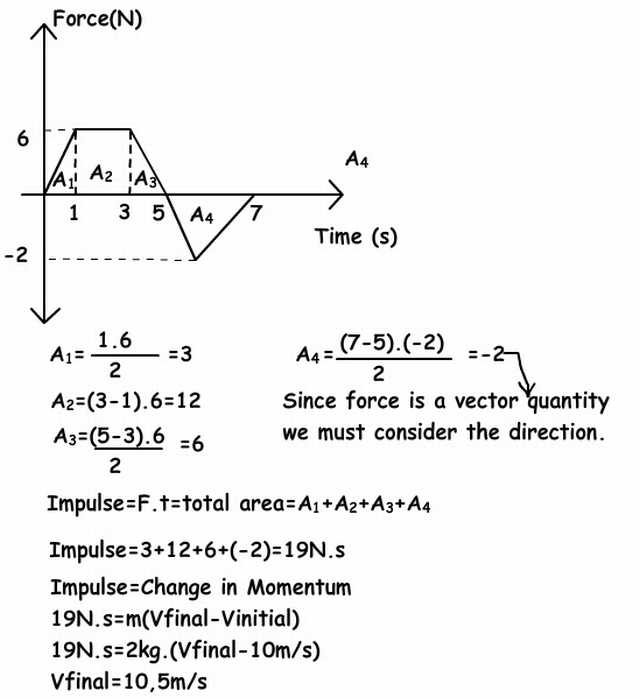
\includegraphics[scale=0.5]{Images/CC/P-Graphs/4.1e/Images/LawsOfMotion/eample46solution}%
\end{minipage}}

\strong{Example} : Suppose a force,$F(t)=6t^{2}-3t+1$, acts on an
7-kg mass for three seconds.

\doublebox{\begin{minipage}[t]{0.72\columnwidth}%
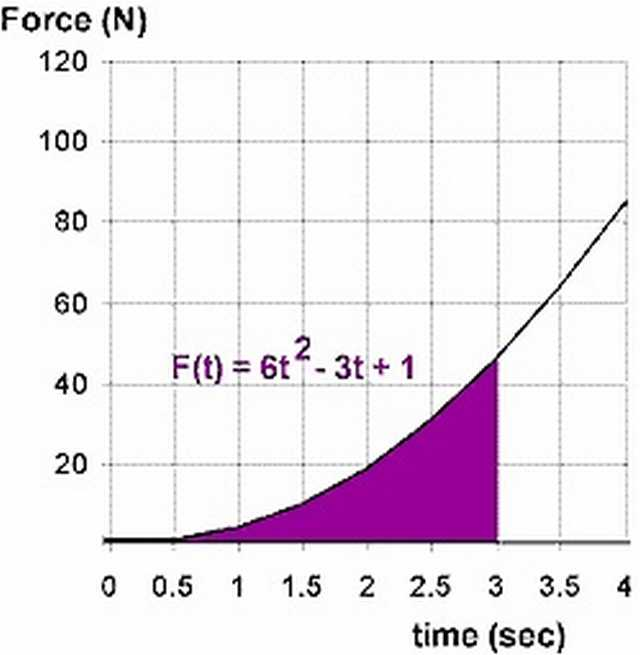
\includegraphics[scale=0.5]{Images/CC/P-Graphs/4.1e/Images/LawsOfMotion/14472c80-cdb1-4390-ba60-eb4a609254b6}%
\end{minipage}}

a) What impulse will the 7-kg object receive in the first three seconds?

b) If the mass started from rest, what is its final velocity? 

Solution : Force as the rate of change of momentum The impulse equation
J = (net F)t = \textgreek{D}p where p = mv can be rearranged to state
that the applied net force applied to an object equals the rate of
change of the its momentum. 

net F = $\dfrac{\triangle p}{\triangle t}$

net F = $\dfrac{m\triangle v}{\triangle t}$

net F = ma

\doublebox{\begin{minipage}[t]{0.72\columnwidth}%
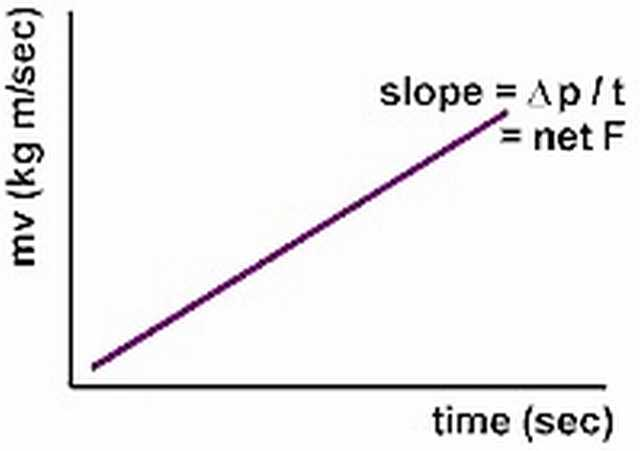
\includegraphics[scale=0.5]{Images/CC/P-Graphs/4.1e/Images/LawsOfMotion/68302de1-5791-4eab-a050-71942cd43ec0}%
\end{minipage}}

That is, the net force acting on an object can be calculated as the
slope of a momentum vs time graph. In terms of the calculus, this
result equates to taking the derivative. 

$\dfrac{dp(t)}{dt}=F(t)$

Notice that force must expressed as a function in terms of time, not
displacement. Calculus will allow us to determine expressions for
instantaneous, non-constant forces and thus is applicable to a wider
range of situations. Let's work an example using this relationship. 

Using the graph provided below, determine the instantaneous force
acting on the 7-kg mass at each of the specified times:

\doublebox{\begin{minipage}[t]{0.72\columnwidth}%
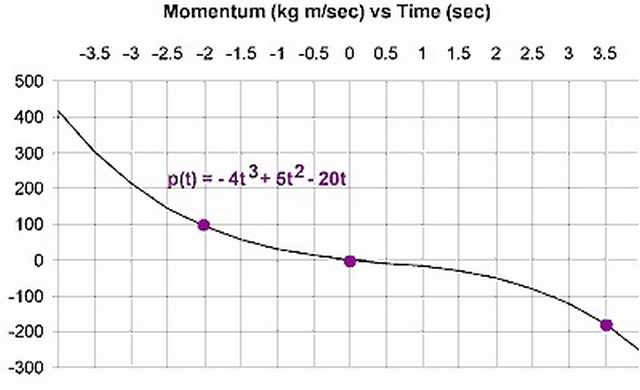
\includegraphics[scale=0.5]{Images/CC/P-Graphs/4.1e/Images/LawsOfMotion/e38a2cef-0533-454a-aac7-69e5c31eec78}%
\end{minipage}}

t = -2 seconds, 

t = 0 seconds, 

t = 3.5 seconds.

\doublebox{\begin{minipage}[t]{0.72\columnwidth}%
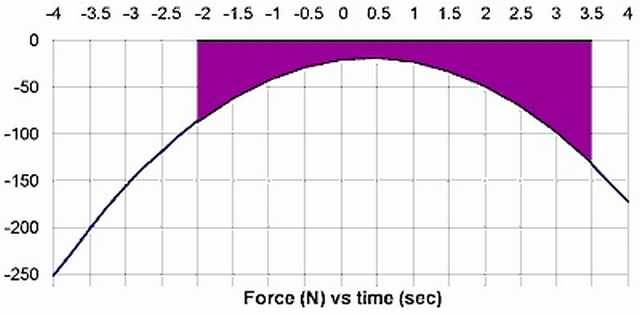
\includegraphics[scale=0.5]{Images/CC/P-Graphs/4.1e/Images/LawsOfMotion/35fe4c31-6a03-4f74-bace-2a4809afc836}%
\end{minipage}}

\strong{Example} : The force shown in the force vs time graph below
acts on a 1.7 kg object.

\doublebox{\begin{minipage}[t]{0.72\columnwidth}%
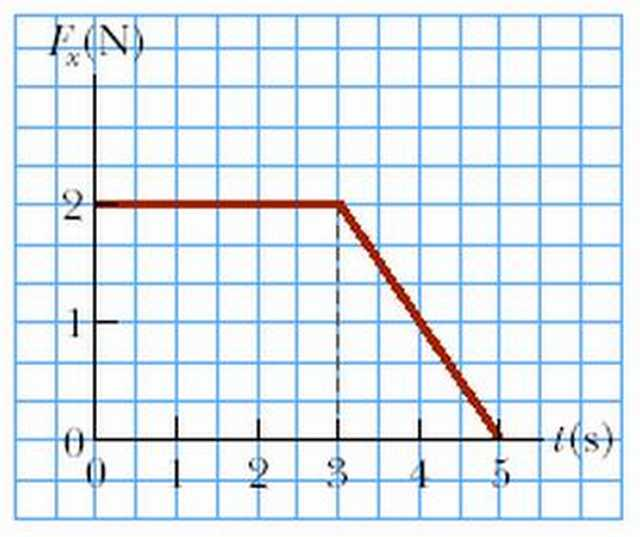
\includegraphics[scale=0.5]{Images/CC/P-Graphs/4.1e/Images/EnergyConservation/impulse-graph}%
\end{minipage}}

(a) Find the magnitude of the impulse of the force. 

Ans : 8 kg m/s.

(b) Find the final velocity of the object if the object was initially
at rest. 

Ans : 2.76 m/s

(c) Find the final velocity of the object if the object was initially
moving along the x axis with a velocity of -1.7 m/s. 

Ans : `` ``

Note : The force shown in the force vs time graph below acts on a
1.7 kg object. Find the final velocity of the object if the object
was initially at rest. Find the final velocity of the object if the
object was initially moving along the x axis with a velocity of -1.7
m/s.

\strong{Example} : Relating Momentum and Impulse 

EXPLORATION \textendash{} An impulsive bike ride Suki is riding her
bicycle, in a straight line, along a flat road. Suki and her bike
have a combined mass of 50 kg. At t = 0, Suki is traveling at 8.0
m/s. Suki coasts for 10 seconds, but when she realizes she is slowing
down, she pedals for the next 20 seconds. Suki pedals so that the
static friction force exerted on the bike by the road increases linearly
with time from 0 to 40 N, in the direction Suki is traveling, over
that 20-second period. Assume there is constant 10 N resistive force,
from air resistance and other factors, acting on her and the bicycle
the entire time. Step 1 - Sketch a diagram of the situation. The diagram
is shown in Figure 6.2, along with the free-body diagram that applies
for the first 10 s and the free-body diagram that applies for the
20second period while Suki is pedaling. 

\doublebox{\begin{minipage}[t]{0.72\columnwidth}%
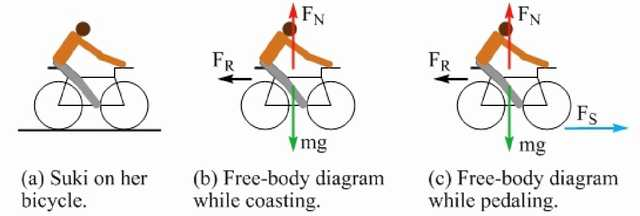
\includegraphics[scale=0.5]{Images/CC/P-Graphs/4.1e/Images/LawsOfMotion/fig2}%
\end{minipage}}

Figure : A diagram of (a) Suki on her bike, as well as free-body diagrams
while she is (b) coasting and while she is (c) pedaling. Note that
in free-body diagram (c), the static friction force $\overset{\rightarrow}{F_{S}}$
gradually increases because of the way Suki pedals. 

Step 2 - Sketch a graph of the net force acting on Suki and her bicycle
as a function of time. Take the positive direction to be the direction
Suki is traveling. In the vertical direction, the normal force exactly
balances the force of gravity, so we can focus on the horizontal forces.
For the first 10 seconds, we have only the 10 N resistive force, which
acts to oppose the motion and is thus in the negative direction. For
the next 20 seconds, we have to account for the friction force that
acts in the direction of motion and the resistive force. We can account
for their combined effect by drawing a straight line that goes from
\textendash 10 N at t = 10 s, to +30 N (40 N \textendash{} 10N) at
t = 30 s. The result is shown in Figure 6.3. 

\doublebox{\begin{minipage}[t]{0.72\columnwidth}%
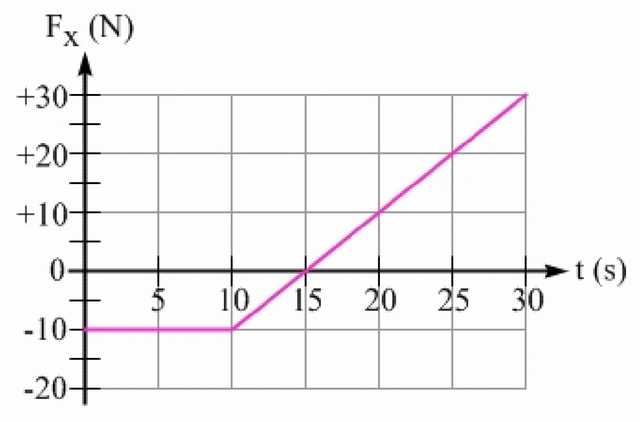
\includegraphics[scale=0.5]{Images/CC/P-Graphs/4.1e/Images/LawsOfMotion/fig3}

Figure 6.3: A graph of the net force acting on Suki and her bicycle
as a function of time. %
\end{minipage}}

Step 3 - What is Suki\textquoteright s speed at t = 10 s? Let\textquoteright s
apply Equation 6.3, which we can write as: 

$\overset{\rightarrow}{F_{net}}\text{\ensuremath{\Delta}}t=\text{\ensuremath{\Delta}}(m\overset{\rightarrow}{v})=m\text{\ensuremath{\Delta}}\overrightarrow{v}=m(\overrightarrow{v_{10s}}-\overrightarrow{v_{i}})$
. 

Solving for the velocity at t = 10 s gives: 

$\overrightarrow{v_{10s}}=\overrightarrow{v_{i}}+\dfrac{\overrightarrow{F_{net}}\triangle t}{m}=+8.0m/s+\dfrac{(-10N)(10s)}{50kg}=+8.0m/s-2.0m/s=+6.0m/s$

Thus, Suki\textquoteright s speed at t = 10 s is 6.0 m/s. We can also
obtain this result from the forceversus-time graph, by recognizing
that the impulse, $\overrightarrow{F_{net}}\text{\ensuremath{\Delta}}t$
, represents the area under this graph over some time interval \ensuremath{\Delta}t
. Let\textquoteright s find the area under the graph, over the first
10 seconds, shown highlighted in green in Figure 6.4. The area is
negative, because the net force is negative over that time interval.
The area under the graph is the impulse:

$\overrightarrow{F_{net}}\text{\ensuremath{\Delta}}t=-10N\times10s=-100Ns=-100kg\;m/s$

Figure 6.4: The green rectangle represents the area under the graph
for the first 10 s. The area is negative, because the force is negative.
From Equation 6.3, we know the impulse is equal to the change in momentum. 

\doublebox{\begin{minipage}[t]{0.72\columnwidth}%
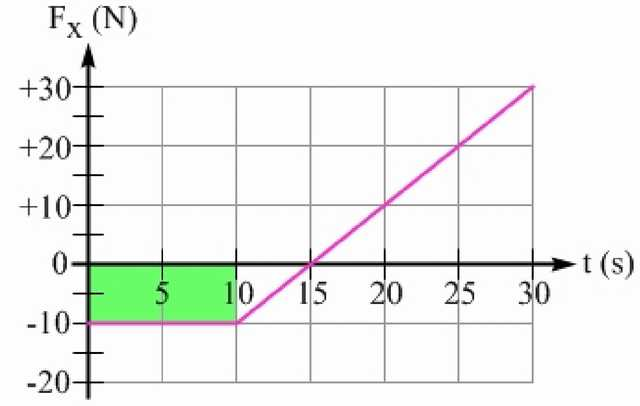
\includegraphics[scale=0.5]{Images/CC/P-Graphs/4.1e/Images/LawsOfMotion/pic6}%
\end{minipage}}

Suki\textquoteright s initial momentum is 

$m\overrightarrow{v_{i}}=50kg\times8.0m/s=+400kg\;m/s$ . Her momentum
at t = 10 s is therefore + 400kg m/s - 100kg m/s = + 300kg m/s . Dividing
this by the mass to find the velocity at t = 10 s confirms what we
found above: 

$\overrightarrow{v}_{10s}=\dfrac{\overrightarrow{p_{10s}}}{m}=\dfrac{\overrightarrow{p_{i}}+\triangle\overrightarrow{p}}{m}=\dfrac{+400kgm/s-100kgm/s}{50kg}=\dfrac{+300kgm/s}{50kg}=+6.0m/s$

Step 4 - What is Suki\textquoteright s speed at t = 30 s? Let\textquoteright s
use the area under the force-versus-time graph, between t = 10 s and
t = 30 s, to find Suki\textquoteright s change in momentum over that
20-second period. This area is highlighted in Figure 6.5, split into
a negative area for the time between t = 10 s and t = 15 s, and a
positive area between t = 15 s and t = 30 s. These regions are triangles,
so we can use the equation for the area of a triangle, 0.5 \texttimes{}
base \texttimes{} height . The area under the curve, between 10 s
and 15 s, is 0.5 \texttimes{} (5.0s) \texttimes ( - 10 N) = - 25kg
m/s . The area between 15 s and 30 s is 0.5 \texttimes{} (15s) \texttimes{}
(30 N) = + 225kg m/s . The total area (total change in momentum) is
+200 kg m/s. 

Note that another approach is to multiply the average net force acting
on Suki and the bicycle (+10 N) over this interval, by the time interval
(20 s), for a +200 kg m/s change in momentum. 

Figure 6.5: The shaded regions correspond to the area under the curve
for the time interval from t = 10 s to t = 30 s. 

\doublebox{\begin{minipage}[t]{0.72\columnwidth}%
\includegraphics[scale=0.5]{Images/CC/P-Graphs/4.1e/Images/LawsOfMotion/pic7}%
\end{minipage}}

In step 3, we determined that Suki\textquoteright s momentum at t
= 10 s is +300 kg m/s. With the additional 200 kg m/s, the net momentum
at t = 10 s is +500 kg m/s. Dividing by the 50 kg mass gives a velocity
at t = 30 s of +10 m/s. 

Key idea for the graphical interpretation of impulse: The area under
the net force versus time graph for a particular time interval is
equal to the change in momentum during that time interval. 

\chapter{Problems for Practice}

\section{General Problem Set}

\subsection{Single Answer Type}
\begin{description}
\item [{Example}] : The relationship between the force F and position x
of a body is as shown in figure. The work done in displacing the body
from x=1m to x=5m will be
\item [{%
\doublebox{\begin{minipage}[t]{0.7\columnwidth}%
\includegraphics[scale=0.5]{\string"Images/CC/P-Graphs/4.1e/Images/LawsOfMotion/ImagesReduced/Scan_20170409 (2)\string".jpg}%
\end{minipage}}}]~
\end{description}
\begin{quote}
a) 30 J

b) 15 J

c) 25 J

d) 20 J

\{ Hint : Area under the graph from 1 to 5 taking signs , 15 J\}
\end{quote}
\begin{description}
\item [{Example:}] A particle of mass m, initially at rest, is acted upon
by a variable force F for a brief interval of time T. It begins to
move with a velocity u after the force stops acting. F is shown in
the graph as a function of time. The curve is a semicircle
\item [{%
\doublebox{\begin{minipage}[t]{0.7\columnwidth}%
\includegraphics[scale=0.5]{Images/CC/P-Graphs/4.1e/Images/LawsOfMotion/ImagesReduced/Scan_20170418}%
\end{minipage}}}]~
\end{description}
\begin{quote}
a) $u=\dfrac{\pi F_{0}^{2}}{2m}$

b) $u=\dfrac{\pi T^{2}}{8m}$

c) $u=\dfrac{\pi F_{0}T}{4m}$

d) $u=\dfrac{F_{0}T}{2m}$

\{ Hint : From impulse relation , $mv_{f}=\dfrac{\pi F_{0}^{2}}{2}$.
So, a, b,c\}
\end{quote}

\section{\index{Previous Years IIT Problems}Previous Years IIT Problems}

\subsection{Single Answer}
\begin{description}
\item [{Example:}] A block of mass m is on an inclined plane of angle $\theta$.
The coefficient of friction between the block and the plane is $\mu$and
$tan\theta>\mu$. The block is held stationary by applying a force
P parallel to the plane. The direction of force pointing up the plane
is taken to be positive. As P is varied from $P_{1}=mg\left(sin\theta-\mu cos\theta\right)$
to $P_{2}=mg\left(sin\theta+\mu cos\theta\right)$, the frictional
force f versus P graph will look like
\item [{%
\doublebox{\begin{minipage}[t]{0.7\columnwidth}%
\includegraphics[scale=0.5]{Images/CC/P-Graphs/4.1e/Images/LawsOfMotion/ImagesReduced/001q}%
\end{minipage}}}]~
\item [{%
\doublebox{\begin{minipage}[t]{0.7\columnwidth}%
\includegraphics[scale=0.5]{Images/CC/P-Graphs/4.1e/Images/LawsOfMotion/ImagesReduced/001}%
\end{minipage}}}]~
\end{description}
\begin{quote}
\{ Solution: Case I : $P_{1}=mg\left(sin\theta-\mu cos\theta\right)$

Case II: $P_{2}=mg\left(sin\theta+\mu cos\theta\right)$

\doublebox{\begin{minipage}[t]{0.7\columnwidth}%
\includegraphics[scale=0.5]{Images/CC/P-Graphs/4.1e/Images/LawsOfMotion/ImagesReduced/001ans}%
\end{minipage}}

In case a), frictional force f is positive and in case b), f is negative.
When $P=mgsin\theta$,$f=\mu mgcos\theta=0$

When $P<mgsin\theta$ ,$f=mgsin\theta-P$

When $P>mgsin\theta$ ,$f=P-mgsin\theta$

Thus f vaires linearly with P, is positive when $P=P_{1}$ and negative
when $P=P_{2}$ . So the correct option is a)

\}
\end{quote}
\begin{comment}
\begin{btSect}[plain]{Bibliography/CC/P-Graphs/4e/lawsofmotion}
\btPrintCited
\end{btSect}
\end{comment}

\printbibliography

\part{\index{Energy Conservation}Energy Conservation}

\chapter{Abstract Introduction}

\section{KINETIC ENERGY }

Objects have energy because of their motion; this energy is called
kinetic energy. Kinetic energy of the objects having mass m and velocity
v can be calculated with the formula given below; 

$E_{k}=\dfrac{1}{2}mv{{}^2}$

As you see from the formula, kinetic energy of the objects is only
affected by the mass and velocity of the objects. The unit of the
$E_{k}$ is again from the formula kg.m\texttwosuperior /s\texttwosuperior{}
or in general use joule. 

\section{Work Done by a Variable Force}

Graphically, the work done on an object or system is equal to the
area under a Force vs. displacement graph: 

\doublebox{\begin{minipage}[t]{0.72\columnwidth}%
\includegraphics[scale=0.5]{Images/CC/P-Graphs/4.1e/Images/EnergyConservation/th1}%
\end{minipage}}

The area under the graph from zero to 20 meters is 300 N m. Thus,
the force represented by the graph does 300 J of work. This work is
also a measure of the energy which was transferred while the force
was being applied

\section{The net force vs. position graph}

The area under the net force vs. position graph represents the change
in kinetic energy (also known as the net work).

\doublebox{\begin{minipage}[t]{0.72\columnwidth}%
\includegraphics[scale=0.5]{Images/CC/P-Graphs/4.1e/Images/EnergyConservation/th4}%
\end{minipage}}

\chapter{Theory and Problems}

\section{Force vs. Distance graph. }

\strong{Example} : Find the kinetic energy of the ball having mass
0,5 kg and velocity 10m/s.

\doublebox{\begin{minipage}[t]{0.72\columnwidth}%
\includegraphics[scale=0.5]{Images/CC/P-Graphs/4.1e/Images/EnergyConservation/topornek}%
\end{minipage}}

Ek=1/2mv\texttwosuperior{} 

Ek=1/2.0, 5. (10) \texttwosuperior{}

Ek=25joule 

As in the case of Kinematics we can use graphs to show the relations
of the concepts here. Look at the given graph of 

\doublebox{\begin{minipage}[t]{0.72\columnwidth}%
\includegraphics[scale=0.5]{Images/CC/P-Graphs/4.1e/Images/EnergyConservation/graphforce}%
\end{minipage}}

Area under the force vs. distance graph gives us work 

Work=Force. Distance=Area=F.X (distance) 

We can find energy of the objects from their Force vs. Distance graph.

\strong{Example} : Find the Kinetic Energy of the object at 14m from
the given graph below. 

\doublebox{\begin{minipage}[t]{0.72\columnwidth}%
\includegraphics[scale=0.5]{Images/CC/P-Graphs/4.1e/Images/EnergyConservation/example28}%
\end{minipage}}

We can find the total kinetic energy of the object after 14m from
the graph; we use area under it to find energy.

\doublebox{\begin{minipage}[t]{0.72\columnwidth}%
\includegraphics[scale=0.5]{Images/CC/P-Graphs/4.1e/Images/EnergyConservation/example28solutionson}%
\end{minipage}}

\chapter{Practice Problems}

\section{General Problem Set}
\begin{description}
\item [{Example}] : A force F acting on an object varies with distance
x as shown in Figure. The force is in newton (N) and the distance
(x) in metre. The work done by the force in moving from x=0 to x=6m
is
\item [{%
\doublebox{\begin{minipage}[t]{0.7\columnwidth}%
\includegraphics[scale=0.5]{\string"Images/CC/P-Graphs/4.1e/Images/EnergyConservation/ImagesReduced/Scan_20170409 (2) FX\string".jpg}%
\end{minipage}}}]~
\end{description}
\begin{quote}
a) 4.5 J

b) 9.0 J

c) 14.5 J

d) 15 J
\end{quote}
\begin{description}
\item [{Example}] : Given below is a graph between a variable force (F)
(along y-axis) and the displacement (X) (along x-axis) of a particle
in one dimension. The work done by the force in the displacement interval
between 0 m and 30 m is
\item [{%
\doublebox{\begin{minipage}[t]{0.7\columnwidth}%
\includegraphics[scale=0.5]{\string"Images/CC/P-Graphs/4.1e/Images/EnergyConservation/ImagesReduced/Scan_20170409 (3)\string".jpg}%
\end{minipage}}}]~
\end{description}
\begin{quote}
a) 275 J

b) 375 J

c) 400 J

d) 300 J
\end{quote}

\section{\index{Previous Years IIT Problems}Previous Years IIT Problems}

\subsection{Single Answer}
\begin{description}
\item [{Example:}] A block of mass 2 kg is free to move along the x-axis.
It is at rest and from t=0 onwards it is subjected to a time-dependent
force F(t) in the x direction. The force F(t) varies with t as shown
in the figure. The kinetic energy of the block after 4.5 seconds is
\item [{%
\doublebox{\begin{minipage}[t]{0.7\columnwidth}%
\includegraphics[scale=0.5]{Images/CC/P-Graphs/4.1e/Images/EnergyConservation/ImagesReduced/002}%
\end{minipage}}}]~
\end{description}
\begin{quote}
a) 4.50J

b) 7.50J

c) 5.06J

d) 14.06J
\end{quote}

\chapter{Review Questions I}

Refer to the following information for the next thirteen questions.
\cite{dev.physicslab.org}

A 5.0-kg mass is pushed along a straight line by a net force described
in the graph below. The object is at rest at t = 0 and x = 0.

\doublebox{\begin{minipage}[t]{0.72\columnwidth}%
\includegraphics[scale=0.5]{Images/CC/P-Graphs/4.1e/Images/EnergyConservation/0406768d-b992-4a57-9d87-a50f2b36ebc3}%
\end{minipage}}

a) During which displacement interval was the object's acceleration
uniform? 

b) What acceleration did the object experience when x = 10 meters? 

c) How much work was done on the object during the first 20 meters? 

d) How much kinetic energy did the object gain during the first 20
meters? 

e) What was the object's instantaneous velocity at x = 20 meters? 

f) How much time was required to move it through the first 20 meters? 

g) How much did the object's momentum change in the first 20 meters? 

h) What was the object's instantaneous acceleration at x = 22 meters? 

i) Why can't the kinematics equations for uniformly accelerated motion
be used to calculate the object's instantaneous velocity at x = 30
meters? What method should be used? 

j) How much work was done to move the object from 20 meters to 30
meters? 

k) What was the object's instantaneous speed at x = 30 meters? 

l) What was the total impulse delivered to the object from x = 0 to
x = 30 meters? 

m) What percent of the impulse was delivered in the last 10 meters? 

\begin{comment}
\begin{btSect}[plain]{Bibliography/CC/P-Graphs/4e/energyconservation}
\btPrintCited
\end{btSect}
\end{comment}

\printbibliography

\part{\index{Rotatory Motion}Rotatory Motion}

\chapter{Problems for Practice}

\section{General Problem Set}

\subsection{Single Answer Type}

\textbf{Example : }The angular velocity of a rotating disc decreases
linearly with angular displacement from 60 rev/min. to zero during
10 rev as shown. Determine the angular velocity of the disc 3 sec
after it begins to slow down

\doublebox{\begin{minipage}[t]{0.7\columnwidth}%
\includegraphics[scale=0.75]{Images/CC/P-Graphs/Common/Reduced/RotatoryMotion/rotation-u1}%
\end{minipage}}

(a) $\dfrac{20\pi}{10}$ 

(b) $\dfrac{17\pi}{10}$ 

(c) $\dfrac{7\pi}{3}$

(d) $\dfrac{10\pi}{3}$

\{ Hint: Answer C \}
\begin{description}
\item [{Example:}] Moment of Inertia I of a solid sphere about an axis
parallel to a diameter and at a distance x from its centre of mass
varies as
\item [{%
\doublebox{\begin{minipage}[t]{0.7\columnwidth}%
\includegraphics[scale=0.5]{Images/CC/P-Graphs/4.1e/Images/RotatoryMotion/ImagesReduced/007}%
\end{minipage}}}]~
\item [{Example:}] A wheel is rolling without sliding on a horizontal surface.
The centre of the wheel moves with a constant speed $v_{o}$ . Consider
a point P on the ri which is at the top at time t=0. The square of
speed of point P is plotted against time t. The correct plot is (
R is radius of the wheel )
\item [{%
\doublebox{\begin{minipage}[t]{0.7\columnwidth}%
\includegraphics[scale=0.5]{Images/CC/P-Graphs/4.1e/Images/RotatoryMotion/ImagesReduced/008}%
\end{minipage}}}]~
\item [{Example:}] A rod of mass m and length l is hinged at one of its
end A as shown in figure. 
\item [{%
\doublebox{\begin{minipage}[t]{0.7\columnwidth}%
\includegraphics[scale=0.5]{Images/CC/P-Graphs/4.1e/Images/RotatoryMotion/ImagesReduced/009-a}%
\end{minipage}}}]~
\end{description}
A force F is applied at a distance x from A. The acceleration of centre
of mass (a) varies with x as

\doublebox{\begin{minipage}[t]{0.7\columnwidth}%
\includegraphics[scale=0.5]{Images/CC/P-Graphs/4.1e/Images/RotatoryMotion/ImagesReduced/009}%
\end{minipage}}
\begin{description}
\item [{Example:}] A circular platform is free to rotate in a horizontal
plane about a vertical axis passing through its centre. A tortoise
is sitting at the edge of the platform. Now the platform is given
an angular velocity $\omega_{o}$. When the tortoise move along a
chord of the platform with a constant velocity ( with respect to the
platform ). The angular velocity of the platform $\omega(t)$ will
vary with time t as
\item [{%
\doublebox{\begin{minipage}[t]{0.7\columnwidth}%
\includegraphics[scale=0.5]{Images/CC/P-Graphs/4.1e/Images/RotatoryMotion/ImagesReduced/010}%
\end{minipage}}}]~
\item [{Example:}] The curve for the moment of inertia of a sphere of constant
mass M versus its radius of gyration K will be
\item [{%
\doublebox{\begin{minipage}[t]{0.7\columnwidth}%
\includegraphics[scale=0.5]{\string"Images/CC/P-Graphs/4.1e/Images/RotatoryMotion/ImagesReduced/Scan_20170409 (2)\string".jpg}%
\end{minipage}}}]~
\item [{\{}] Hint : a) \}
\item [{Example}] : The graph between rotational energy $E_{r}$ and angular
velocity $\omega$ is represented by which curve 
\item [{%
\doublebox{\begin{minipage}[t]{0.7\columnwidth}%
\includegraphics[scale=0.5]{\string"Images/CC/P-Graphs/4.1e/Images/RotatoryMotion/ImagesReduced/Scan_20170409 (2)_2\string".jpg}%
\end{minipage}}}]~
\item [{\{}] Hint : a) \}
\item [{Example}] : The curve between angular momentum L and angular velocity
$\omega$ will be
\item [{%
\doublebox{\begin{minipage}[t]{0.7\columnwidth}%
\includegraphics[scale=0.5]{\string"Images/CC/P-Graphs/4.1e/Images/RotatoryMotion/ImagesReduced/Scan_20170409 (2)_3\string".jpg}%
\end{minipage}}}]~
\item [{\{}] Hint : a) \}
\end{description}

\chapter{\index{Angular Momentum Conservation}Angular Momentum Conservation}
\begin{description}
\item [{Example}] : A block slides on a rough horizontal ground from point
A to point B. Point C is midway between A and B. The coefficient of
friction between the block and the ground is constant. Its angular
momentum L about C is plotted against time t. Which of the following
curves is correct?
\item [{%
\doublebox{\begin{minipage}[t]{0.7\columnwidth}%
\includegraphics[scale=0.5]{\string"Images/CC/P-Graphs/4.1e/Images/Momentum/ImagesReduced/Scan_20170418 (3)\string".jpg}%
\end{minipage}}}]~
\end{description}

\part{\index{Gravitation}Gravitation}

\chapter{Basics}

\section{Variation of ``g''}

Outside the earth $g=g_{o}\left(\dfrac{R}{r}\right)^{2}$

where $g_{o}$ is the acceleration due to gravity at the surface of
earth.

\doublebox{\begin{minipage}[t]{0.7\columnwidth}%
\includegraphics[scale=0.5]{Images/CC/P-Graphs/4.1e/Images/Gravitation/ImagesReduced/g}%
\end{minipage}}

$g_{o}=\dfrac{GM}{R^{2}}$ , R = radius of earth

\chapter{Problems for Practice}

\section{General Problem Set}

\subsection{Single Answer}
\begin{description}
\item [{Example:}] A sphere of mass M and radius $R_{2}$ has a concentric
cavity of radius $R_{1}$ as shown in figure. 
\end{description}
\doublebox{\begin{minipage}[t]{0.7\columnwidth}%
\includegraphics[scale=0.5]{Images/CC/P-Graphs/4.1e/Images/Gravitation/ImagesReduced/002g}%
\end{minipage}}

The force F exerted by the sphere on a particle of mass m located
at a distance r from the centre of sphere varies as ($0\leq r\leq\infty$) 

\doublebox{\begin{minipage}[t]{0.7\columnwidth}%
\includegraphics[scale=0.5]{\string"Images/CC/P-Graphs/4.1e/Images/Gravitation/ImagesReduced/002-a g\string".jpg}%
\end{minipage}}
\begin{description}
\item [{Example}] : The variation of acceleration due to gravity as one
moves away from earth's centre is given by the graph
\item [{%
\doublebox{\begin{minipage}[t]{0.7\columnwidth}%
\includegraphics[scale=0.5]{\string"Images/CC/P-Graphs/4.1e/Images/Gravitation/ImagesReduced/Scan_20170409 (6)\string".jpg}%
\end{minipage}}}]~
\item [{\{}] Hint: c) \}
\item [{Example}] : Which of the following graphs represents the motion
of a planet moving about the sun?
\item [{%
\doublebox{\begin{minipage}[t]{0.7\columnwidth}%
\includegraphics[scale=0.5]{\string"Images/CC/P-Graphs/4.1e/Images/Gravitation/ImagesReduced/Scan_20170409 (6)_2\string".jpg}%
\end{minipage}}}]~
\item [{\{}] Hint : a) \}
\item [{Example}] : P is a point at a distance r from the centre of a solid
sphere of radius a. The gravitational potential at P is V. If V is
plotted as a function of r, which is the correct curve?
\item [{%
\doublebox{\begin{minipage}[t]{0.7\columnwidth}%
\includegraphics[scale=0.5]{\string"Images/CC/P-Graphs/4.1e/Images/Gravitation/ImagesReduced/Scan_20170409 (7)\string".jpg}%
\end{minipage}}}]~
\item [{\{}] Hint : c) \}
\item [{Example}] : Which of the graphs represents correctly the variation
of intensity of gravitational field I with the distance r from the
centre of a spherical shell of mass M and radius a?
\item [{%
\doublebox{\begin{minipage}[t]{0.7\columnwidth}%
\includegraphics[scale=0.5]{\string"Images/CC/P-Graphs/4.1e/Images/Gravitation/ImagesReduced/Scan_20170409 (7)_2\string".jpg}%
\end{minipage}}}]~
\item [{\{}] Hint : d) \}
\item [{Example}] : The dependence of acceleration due to gravity g on
the distance r from the center of the earth, assumed to be a sphere
of radius R of uniform density is as shown in figure below
\item [{%
\doublebox{\begin{minipage}[t]{0.7\columnwidth}%
\includegraphics[scale=0.5]{Images/CC/P-Graphs/4.1e/Images/Gravitation/ImagesReduced/Scan_20170409_73}%
\end{minipage}}}]~
\end{description}

\subsection{Multiple Answer}
\begin{description}
\item [{Example:}] Two concentric spherical shells are as shown in figure.
The magnitude of gravitational potential (V) and field strength (E)
vary with distance (r) from centre as
\end{description}
\doublebox{\begin{minipage}[t]{0.7\columnwidth}%
\includegraphics[scale=0.5]{Images/CC/P-Graphs/4.1e/Images/Gravitation/ImagesReduced/001a}%
\end{minipage}}

\doublebox{\begin{minipage}[t]{0.7\columnwidth}%
\includegraphics[scale=0.5]{Images/CC/P-Graphs/4.1e/Images/Gravitation/ImagesReduced/001}%
\end{minipage}}

\subsection{Comprehension Type}

\subsubsection{Concept 1 Gravitational potential inside a sphereical shell is constant
and outside the shell it varies as $V\propto\dfrac{1}{r}$ (with negative
sign). Here r is the distance from centre.}

\doublebox{\begin{minipage}[t]{0.7\columnwidth}%
\includegraphics[scale=0.5]{Images/CC/P-Graphs/4.1e/Images/Gravitation/ImagesReduced/Scan_20170407}%
\end{minipage}}
\begin{description}
\item [{Example1:}] Two concentric spherical shells are as shown in figure.
The V-r graph will be as
\end{description}
\doublebox{\begin{minipage}[t]{0.7\columnwidth}%
\includegraphics[scale=0.5]{Images/CC/P-Graphs/4.1e/Images/Gravitation/ImagesReduced/Gravitation_AR1}%
\end{minipage}}

Statement : 1: Gravitational Field at distance x from the centre on
the axis of a ring is given as

$E=\dfrac{Gmx}{\left(R^{2}+x^{2}\right)^{3/2}}$

Here m is the mass of ring and R its radius.

2: Gravitational field at distance x($\geq R$) from centre of a solid
sphere is given as, 

$E=\dfrac{Gm}{x^{2}}$

Here m is the mass of solid sphere.
\begin{description}
\item [{Example2:}] One ring of radius R and mass m and one solid sphere
of same mass m and same radius R are placed with their centres on
positive x-axis. We are moving from some finite distance on negative
x-axis towards positive x-axis. Plane of the ring is perpendicular
to x-axis. How will the net gravitational field vary with distance
moved on x-axis. We move only up to surface of solid sphere. O is
the origin,
\item [{%
\doublebox{\begin{minipage}[t]{0.7\columnwidth}%
\includegraphics[scale=0.5]{Images/CC/P-Graphs/4.1e/Images/Gravitation/ImagesReduced/Gravitation_AR2_Q}%
\end{minipage}}}]~
\item [{%
\doublebox{\begin{minipage}[t]{0.7\columnwidth}%
\includegraphics[scale=0.5]{Images/CC/P-Graphs/4.1e/Images/Gravitation/ImagesReduced/Gravitation_AR2_answer}%
\end{minipage}}}]~
\item [{Statement:}] Change in potential energy when a mass m is taken
to a height h from the surface of earth is given by 
\end{description}
$\triangle U=\dfrac{mgh}{1+h/R}$

\section{\index{Previous Years IIT Problems}Previous Years IIT Problems}

\subsection{Single Answer}

A spherically symmetric gravitational system of particles has a mass
density 

$\rho=\begin{cases}
\rho_{o} & for\;r\leq R\\
0 & for\;r>R
\end{cases}$

where $\rho_{o}$ is a constant. A test mass can undergo circular
motion under the influence of the gravitational field of particles.
Its speed v as a function of distance r ( $0<r<\infty$) from the
centre of the system is represented by 

\doublebox{\begin{minipage}[t]{0.7\columnwidth}%
\includegraphics[scale=0.5]{Images/CC/P-Graphs/4.1e/Images/Gravitation/ImagesReduced/007}%
\end{minipage}}

\{Solution: If M is the total mass of the system of particles, the
orbital speed of the test mass is

$v=\sqrt{\dfrac{GM}{r}}$

For $r\leq R,$ $v=\sqrt{\dfrac{G\times\dfrac{4\pi}{3}r^{3}\rho_{o}}{r}}$
which gives $v\propto r$

i.e. v increases linearly with r up to r=R. Hence choices b) and d)
are wrong.

For r\textgreater R, the whole mass of the system is $M=\dfrac{4\pi}{3}R^{3}\rho_{o}$,
which is constant. Hence for r\textgreater R, 

$v=\sqrt{\dfrac{GM}{r}}$

i.e, $v\propto\dfrac{1}{\sqrt{r}}$. Hence, the correct choice is
c). \}

\subsection{Matching}

\doublebox{\begin{minipage}[t]{0.7\columnwidth}%
\includegraphics[scale=0.5]{Images/CC/P-Graphs/4.1e/Images/Gravitation/ImagesReduced/002}%
\end{minipage}}

\part{\index{Periodic Motion}Periodic Motion}

\chapter{Abstract Introduction (\index{SHM}SHM)}

\section{Position vs time }

The graph of position verse time is a sine wave with a possible phase
shift. The phase shift is how much the ahead or behind the position
is on the sine wave. \cite{ipodphysics.com}

\doublebox{\begin{minipage}[t]{0.72\columnwidth}%
\includegraphics[scale=0.5]{\string"Images/CC/P-Graphs/4.1e/Images/SHM/Sine wave\string".JPG}%
\end{minipage}}

Consider this graph, if the \textquotedbl clock\textquotedbl{} is
started at 0.05 (where the mass is at it's maximum stretch) seconds
then there would be a phase shift of 90 degrees (or we could replace
the sine function for a cosine). If the \textquotedbl clock\textquotedbl{}
is started at 0.1 seconds (where mass moves down instead of up; left
instead of right) then the phase shift would be 180 degrees (a negative
sine function).

\section{Velocity vs time}

Consider the position verses time graph, at any point were the mass
has reached the amplitude (maximum distance from from the equilibrium
point) the speed of the mass at these point is zero. When the position
is at zero then the speed is at a maximum (if you don't believe it,
consider conservation of energy). This \textquotedbl shifts\textquotedbl{}
the position graph by 90 degrees \textquotedbl creating\textquotedbl{}
a cosine graph for velocity. The other way of thinking about is velocity
is the change in position with respect to time, the change in a sine
wave with respect to time is a cosine graph.

\doublebox{\begin{minipage}[t]{0.72\columnwidth}%
\includegraphics[scale=0.5]{\string"Images/CC/P-Graphs/4.1e/Images/SHM/cosine wave\string".JPG}%
\end{minipage}}

\section{Acceleration vs time}

The acceleration verse time graph is the easiest of the graphs to
make. The simple harmonic motion is based on a relationship between
position and acceleration; x = - Ka. So the graph of position and
acceleration should look alike, except for the negative sign. In fact
position and acceleration are the same shape just mirror copies of
each other. 

\doublebox{\begin{minipage}[t]{0.72\columnwidth}%
\includegraphics[scale=0.5]{Images/CC/P-Graphs/4.1e/Images/SHM/-sinewave.JPG}%
\end{minipage}}

\subsection{Peak Height}

It is important to note that the shapes of each graph is simular,
that each graph has the same frequency, period and wavelength, but
they don't have the same amplitude, for common simple harmonic motion,
the height the peak of the function (not to confused with the amplitude,
amplitude refers to the height of the position graph alone, i'm talking
about the height of the position, velocity and acceleration graphs)
tend to get smaller and smaller starting with the position graph being
the tallest and the acceleration being the shortest.

\section{Graphing position, velocity, and acceleration with respect to each
other}

Graphing position to the other functions can be complicated and when
tested on it, most student are unable to give the right answer. First
consider this, for simple harmonic motion position and acceleration
are proportional. x = -k a this is a linear relationship so the graph
is a line, the slope is negative so the line is heading down. 

\doublebox{\begin{minipage}[t]{0.72\columnwidth}%
\includegraphics[scale=0.5]{Images/CC/P-Graphs/4.1e/Images/SHM/linear}%
\end{minipage}}

\section{Position and acceleration verses velocity}

The position and acceleration verse velocity graph look entirely different.
First off the straight line test fails when plotting position vs velocity
or acceleration verse velocity. Take the point were x and a are zero,
there are two possible answers for the point (the speed maybe at maximum)
the object could be moving down or up at the point. That means the
velocity can be a positive maximum or a negative maximum, two separate
values. Looking a the points were the velocity is equal to zero, there
are two possible answers, either at the top or at the bottom. If you
continue to plot data points graph that is developed is a ellisipe 

\doublebox{\begin{minipage}[t]{0.72\columnwidth}%
\includegraphics[scale=0.5]{Images/CC/P-Graphs/4.1e/Images/SHM/ellipse.JPG}%
\end{minipage}}

\chapter{Problems}

\section{General Problem Set}

\subsection{Single Answer Type}
\begin{description}
\item [{Example}] 1: Aceleration-displacement graph of a particle executing
SHM is as shown in given figure. The time period of its oscillation
is ( in sec )
\item [{%
\doublebox{\begin{minipage}[t]{0.7\columnwidth}%
\includegraphics[scale=0.5]{Images/CC/P-Graphs/4.1e/Images/SHM/ImagesReduced/Scan_20170407_shm_ob1}%
\end{minipage}}}]~
\end{description}
\begin{quote}
a) $\pi/2$

b) $2\pi$

c) $\pi$

d) $\pi/4$
\end{quote}
\begin{description}
\item [{Example}] 2: Displacement-time graph of a particle executing SHM
is as shown. 
\item [{%
\doublebox{\begin{minipage}[t]{0.7\columnwidth}%
\includegraphics[scale=0.5]{Images/CC/P-Graphs/4.1e/Images/SHM/ImagesReduced/Scan_20170407_ob2}%
\end{minipage}}}]~
\item [{%
\doublebox{\begin{minipage}[t]{0.7\columnwidth}%
\includegraphics[scale=0.5]{Images/CC/P-Graphs/4.1e/Images/SHM/ImagesReduced/Scan_20170407_ob_answer}%
\end{minipage}}}]~
\item [{Example}] 3: For a particle executing SHM the displacement x is
given by $x=A\cos\omega t$. Identify the graph which represents the
variation of potential energy (PE) as a function of time t and displacement
x
\item [{%
\doublebox{\begin{minipage}[t]{0.7\columnwidth}%
\includegraphics[scale=0.5]{\string"Images/CC/P-Graphs/4.1e/Images/SHM/ImagesReduced/Scan_20170407 (2) ob3\string".jpg}%
\end{minipage}}}]~
\end{description}
\begin{quote}
a) I, III

b) II, IV

c) II, III

d) I, IV
\end{quote}

\subsection{Multiple Answer Type}
\begin{description}
\item [{Example}] 1: Velocity-time graph of a particle executing SHM is
shown in figure. Select the correct alternative(s).
\item [{%
\doublebox{\begin{minipage}[t]{0.7\columnwidth}%
\includegraphics[scale=0.5]{\string"Images/CC/P-Graphs/4.1e/Images/SHM/ImagesReduced/Scan_20170407 (3) obtype2nd_1\string".jpg}%
\end{minipage}}}]~
\end{description}
\begin{quote}
a) At position 1 displacement of particle may be positive or negative.

b) At position 2 displacement of particle is negative.

c) At position 3 acceleration of particle is positive.

d) At position 4 acceleration of particle is positive.
\end{quote}
\begin{description}
\item [{Example}] 2: Acceleration-time graph of a particle executing SHM
is as shown in figure. Select the correct alternative(s).
\item [{%
\doublebox{\begin{minipage}[t]{0.7\columnwidth}%
\includegraphics[scale=0.5]{\string"Images/CC/P-Graphs/4.1e/Images/SHM/ImagesReduced/Scan_20170407 (3) obtype2nd_2\string".jpg}%
\end{minipage}}}]~
\end{description}
\begin{quote}
a) Displacement of particle at 1 is negative.

b) Velocity of particle at 2 is positive.

c) Potential energy of particle at 3 is maximum.

d) Speed of particle at 3 is decreasing.
\end{quote}

\subsection{Matching Type Questions}
\begin{description}
\item [{Example}] 1: Velocity-time graph of a particle in SHM is as shown
in figure. Match the following
\end{description}
\doublebox{\begin{minipage}[t]{0.7\columnwidth}%
\includegraphics[scale=0.5]{\string"Images/CC/P-Graphs/4.1e/Images/SHM/ImagesReduced/Scan_20170407 (4) Mtch1\string".jpg}%
\end{minipage}}

\doublebox{\begin{minipage}[t]{0.7\columnwidth}%
\includegraphics[scale=0.5]{\string"Images/CC/P-Graphs/4.1e/Images/SHM/ImagesReduced/Scan_20170407 (4) Mtch1_questions\string".jpg}%
\end{minipage}}
\begin{description}
\item [{Example}] 2: F-x and x-t graph of a particle in SHM are as shown
in figure. Match the following
\item [{%
\doublebox{\begin{minipage}[t]{0.7\columnwidth}%
\includegraphics[scale=0.5]{\string"Images/CC/P-Graphs/4.1e/Images/SHM/ImagesReduced/Scan_20170407 (5) Mtching_2\string".jpg}%
\end{minipage}}}]~
\item [{%
\doublebox{\begin{minipage}[t]{0.7\columnwidth}%
\includegraphics[scale=0.5]{\string"Images/CC/P-Graphs/4.1e/Images/SHM/ImagesReduced/Scan_20170407 (5) Mtching_2.2\string".jpg}%
\end{minipage}}}]~
\item [{%
\doublebox{\begin{minipage}[t]{0.7\columnwidth}%
\includegraphics[scale=0.5]{\string"Images/CC/P-Graphs/4.1e/Images/SHM/ImagesReduced/Scan_20170407 (5) Mtching_2.3\string".jpg}%
\end{minipage}}}]~
\end{description}

\subsection{Comprehension Type Questions}

\subsubsection{Comprehension 1}

Concept : In SHM, force $\left(F=-\dfrac{dU}{dr}\right)$ on the particle
at mean position is zero. Potential energy at extreme position is
maximum

Example: U-r graph of a particle which can be under SHM is as shown
in figure. What conclusion cannot be drawn from the graph?

\doublebox{\begin{minipage}[t]{0.7\columnwidth}%
\includegraphics[scale=0.5]{\string"Images/CC/P-Graphs/4.1e/Images/SHM/ImagesReduced/Scan_20170407 (6) Comprehension 1\string".jpg}%
\end{minipage}}

a) Mean position of the particle is at r=2m.

b) Potential energy of particle at mean position is 10 J.

c) Amplitude of oscillation is 1 m.

d) None of these.

\subsubsection{Comprehension 2}

Statement : In case of pure rolling $a=R\alpha$, where a is the linear
acceleration and $\alpha$ the angular acceleration.

Question : A disc of mass m and radius R is attached with a spring
of force constant k at its centre as shown in figure. At x=0, spring
is unstretched. The disc is moved to x=A and then released. There
is no slipping between disc and ground. Let f be the force of friction
on the disc from the ground.

\doublebox{\begin{minipage}[t]{0.7\columnwidth}%
\includegraphics[scale=0.5]{\string"Images/CC/P-Graphs/4.1e/Images/SHM/ImagesReduced/Scan_20170407 Comp\string".jpg}%
\end{minipage}}

Example 1 : f versus t (time) graph will be as

\doublebox{\begin{minipage}[t]{0.7\columnwidth}%
\includegraphics[scale=0.5]{\string"Images/CC/P-Graphs/4.1e/Images/SHM/ImagesReduced/Scan_20170407 Q1Comp\string".jpg}%
\end{minipage}}

Example 2 : In the problem if k = 10 N/m, m= 2 kg, R = 1 m and A =
2 m. Find linear speed of the disc at mean position

a) $\sqrt{\dfrac{40}{3}}$ m/s

b) $\sqrt{20}$ m/s 

c) $\sqrt{\dfrac{10}{3}}$m/s

d) $\sqrt{\dfrac{50}{3}}$ m/s

\section{\index{Previous Years IIT Problems}Previous Years IIT Problems}

\subsection{Paragraph}
\begin{description}
\item [{Paragraph}] 1: When a particle of mass m moves on the x-axis in
a potential of the form $V(x)=kx^{2}$ it performs simple harmonic
motion. The corresponding time period is proportional to $\sqrt{\dfrac{m}{k}}$,
as can be seen easily using dimensional analysis. However, the motion
of a particle can be periodic even when its potential energy increases
on both sides of x=0 in a way different from $kx^{2}$ and its total
energy is such that the particle does not escape to infinity. Consider
a particle of mass m moving on the x-axis. Its potential energy is
$V(x)=\alpha x^{4}$ ($\alpha>0$) for \textbar x\textbar{} near
the origin and becomes a constant equal to Vo for $|x|\geq X_{0}$
(see figure)
\item [{%
\doublebox{\begin{minipage}[t]{0.7\columnwidth}%
\includegraphics[scale=0.5]{Images/CC/P-Graphs/4.1e/Images/SHM/ImagesReduced/002-3}%
\end{minipage}}}]~
\item [{1.}] If the total energy of the particle is E, it will perform
periodic motion only if
\end{description}
\begin{quote}
a) E\textless 0

b) E\textgreater 0

c) Vo\textgreater E\textgreater 0

d) E\textgreater Vo 
\end{quote}
\begin{description}
\item [{2.}] For periodic motion of small amplitude A, the time period
T of this particle is proportional to 
\end{description}
\begin{quote}
a) $A\sqrt{\dfrac{m}{\alpha}}$

b) $\dfrac{1}{A}\sqrt{\dfrac{m}{\alpha}}$

c) $A\sqrt{\dfrac{\alpha}{m}}$

d) $\dfrac{1}{A}\sqrt{\dfrac{\alpha}{m}}$
\end{quote}
\begin{description}
\item [{3.}] The acceleration of this particle for \textbar x\textbar{}
\textgreater{} Xo is
\end{description}
\begin{quote}
a) Proportional to Vo

b) Proportional to Vo/mXo

c) Proportional to $\sqrt{Vo/mXo}$

d) Zero
\end{quote}
\begin{comment}
\begin{btSect}[plain]{Bibliography/CC/P-Graphs/4e/shm}
\btPrintCited
\end{btSect}
\end{comment}

\printbibliography

\part{\index{Statics}Statics}

\chapter{\index{Modulii of Elasticity}Modulii of Elasticity}

\section{General Problem Set}

\subsection{Single Answer Type}

Example 1 : The graph shows the extension ($\triangle l$) of a wire
of length 1.0m suspended from the top of a roof at one end and with
a load W connected to the other end. If the cross-sectional area of
the wire is $10^{-6}m^{2}$, calculate the Young's modulus of the
material of the wire

\doublebox{\begin{minipage}[t]{0.7\columnwidth}%
\includegraphics[scale=0.5]{Images/CC/P-Graphs/4.1e/Images/ModuliiOfElasticity/ImagesReduced/Scan_20170407}%
\end{minipage}}

a) $2\times10^{11}$ $N/m^{2}$

b) $2\times10^{10}$ $N/m^{2}$

c) $2\times10^{12}$ $N/m^{2}$

d) $2\times10^{13}$ $N/m^{2}$

\textbf{Example : }The graph shown was obtained from experimental
measurements of the period of oscillation T for different masses M
placed in the scale pan on the lower end of the spring balance. The
most likely reason for the line not passing through the origin is
that the 

\doublebox{\begin{minipage}[t]{0.7\columnwidth}%
\includegraphics[scale=0.75]{Images/CC/P-Graphs/Common/Reduced/Elasticity/elasticity-e1}%
\end{minipage}}

(a) Spring did not obey Hooke's law

(b) Amplitude of oscillation was too large

(c) Clock used needed regulating

(d) Mass of the pan was neglected

\{ Hint: Answer D \}

\subsection{Comprehension Type}

\subsubsection{Comprehension 1}

Concept : Free body diagram of liquid can be drawn in similar manner
as we draw the free body diagram of a solid. The only difference is,
what we call the normal reaction between solid-solid boundary, we
here call it pressure X area in case of liquids. Both are prependicular
to the surface.

Example : Equal amounts of liquid are filled in two vessels of different
shapes as shown in figure. Let $F_{1}$be the force by the base on
liquid in case (i) and $F_{2}$ in case (ii) Then

\doublebox{\begin{minipage}[t]{0.7\columnwidth}%
\includegraphics[scale=0.5]{\string"Images/CC/P-Graphs/4.1e/Images/ModuliiOfElasticity/ImagesReduced/Scan_20170407 comp1\string".jpg}%
\end{minipage}}

a) $F_{1}$ \textgreater$F_{2}$

b) $F_{1}$ \textless$F_{2}$

c) $F_{1}$ =$F_{2}$

d) Data insufficient

Question : A cube (side = 10 cm ) of density 0.5 $g/cm^{3}$ is placed
in a vessel of base area 20 cm X 20 cm. A liquid of density 1.0 $g/cm^{3}$
is gradually filled in the vessel at a constant rate Q = 50 $cm^{3}/s$.

\doublebox{\begin{minipage}[t]{0.7\columnwidth}%
\includegraphics[scale=0.5]{\string"Images/CC/P-Graphs/4.1e/Images/ModuliiOfElasticity/ImagesReduced/Scan_20170407 comp1_2\string".jpg}%
\end{minipage}}

Example : If we plot a graph between the normal reaction on cube by
the vessel versus time. The graph will be like 

\doublebox{\begin{minipage}[t]{0.7\columnwidth}%
\includegraphics[scale=0.5]{\string"Images/CC/P-Graphs/4.1e/Images/ModuliiOfElasticity/ImagesReduced/Scan_20170407 comp1_3\string".jpg}%
\end{minipage}}

Example: The cube will leave contact with the vessel after time t=
......... s

a) 30

b) 40

c) 60

d) 20

\part*{\index{Heat}Heat}

\part{\index{Thermodynamics}Thermodynamics}

\chapter{Practice Problems}

\section{General Problem Set}

\subsection{Single Answer Type}
\begin{description}
\item [{Example}] : Pressure versus temperature graphs of an ideal gas
are as shown in figure. Choose the wrong statement
\item [{%
\doublebox{\begin{minipage}[t]{0.7\columnwidth}%
\includegraphics[scale=0.5]{\string"Images/CC/P-Graphs/4.1e/Images/Thermodynamics/ImagesReduced/Scan_20170408 (3)\string".jpg}%
\end{minipage}}}]~
\end{description}
\begin{quote}
a) Density of gas is increasing in graph (i)

b) Density of gas is decreasing in graph (ii)

c) Density of gas is constant in graph (iii)

d) None of the above
\end{quote}
\begin{description}
\item [{Example}] : In a cyclic process shown in the figure an ideal gas
is adiabatically taken from B to A, the work done on the gas during
the process B-\textgreater A is 30J, when the gas is taken from A-\textgreater B
the heat absorbed by the gas is 20 J. The change in internal energy
of the gas in the process A-\textgreater{} B is
\item [{%
\doublebox{\begin{minipage}[t]{0.7\columnwidth}%
\includegraphics[scale=0.5]{\string"Images/CC/P-Graphs/4.1e/Images/Thermodynamics/ImagesReduced/Scan_20170408 (4)\string".jpg}%
\end{minipage}}}]~
\item [{Example}] : An ideal monoatomic gas undergoes a cyclic process
ABCA as shown in the figure. The ratio of heat absorbed during AB
to the work done on the gas during BC is
\item [{%
\doublebox{\begin{minipage}[t]{0.7\columnwidth}%
\includegraphics[scale=0.5]{\string"Images/CC/P-Graphs/4.1e/Images/Thermodynamics/ImagesReduced/Scan_20170408 (4)_ob\string".jpg}%
\end{minipage}}}]~
\end{description}
\begin{quote}
a) 5/2ln2

b) 5/3

c) 5/4ln2

d) 5/6
\end{quote}
\begin{description}
\item [{Example}] : Three moles of an ideal monoatomic gas performs a cycle
1-\textgreater 2-\textgreater 3-\textgreater 4-\textgreater 1
as shown. The gas temperatures in different states are T1=400K, T2=800K,
T3=2400K and T4=1200K. The work done by the gas during the cycle is
(2-3 and 4-1 are isobaric)
\item [{%
\doublebox{\begin{minipage}[t]{0.7\columnwidth}%
\includegraphics[scale=0.5]{\string"Images/CC/P-Graphs/4.1e/Images/Thermodynamics/ImagesReduced/Scan_20170408 (4) obnxt\string".jpg}%
\end{minipage}}}]~
\end{description}
\begin{quote}
a) 1200 R

b) 3600 R

c) 2400 R

d) 2000 R
\end{quote}
\begin{description}
\item [{Example}] : Temperature of a body $\theta$ is slightly more than
the temperature of the surrounding $\theta_{o}$ . Its rate of cooling
(R) versus temperature of body ($\theta$) is plotted, its shape would
be
\item [{%
\doublebox{\begin{minipage}[t]{0.7\columnwidth}%
\includegraphics[scale=0.5]{Images/CC/P-Graphs/4.1e/Images/Thermodynamics/ImagesReduced/Scan_20170408}%
\end{minipage}}}]~
\item [{Example}] : Pressure versus density graph of an ideal gas is shown
in figure
\item [{%
\doublebox{\begin{minipage}[t]{0.7\columnwidth}%
\includegraphics[scale=0.5]{Images/CC/P-Graphs/4.1e/Images/Thermodynamics/ImagesReduced/Scan_20170408_ob1}%
\end{minipage}}}]~
\end{description}
\begin{quote}
a) during the process AB work done by the gas is positive

b) during the process AB work done by the gas is negative

c) during the process BC internal energy of the gas is increasing

d) None of the above
\end{quote}
\begin{description}
\item [{Example}] : Ideal gas is taken through the process shown in the
figure
\item [{%
\doublebox{\begin{minipage}[t]{0.7\columnwidth}%
\includegraphics[scale=0.5]{Images/CC/P-Graphs/4.1e/Images/Thermodynamics/ImagesReduced/Scan_20170408_ob2}%
\end{minipage}}}]~
\end{description}
\begin{quote}
a) In process AB, work done by system is positive

b) In process AB, heat is rejected

c) In process AB, internal energy increases

d) In process AB internal energy decreases and in process BC, internal
energy increases
\end{quote}
\begin{description}
\item [{Example}] : A gas is expanded from volume $V_{0}$ to $2V_{0}$
under three different processes. Process 1 is isobaric, process 2
is isothermal and process 3 is adiabatic. Let $\triangle U_{1}$,$\triangle U_{2}$
and $\triangle U_{3}$ be the change in internal energy of the gas
in these three processes. Then
\item [{%
\doublebox{\begin{minipage}[t]{0.7\columnwidth}%
\includegraphics[scale=0.5]{\string"Images/CC/P-Graphs/4.1e/Images/Thermodynamics/ImagesReduced/Scan_20170408 (2)\string".jpg}%
\end{minipage}}}]~
\end{description}
\begin{quote}
a) $\triangle U_{1}$\textgreater$\triangle U_{2}$\textgreater$\triangle U_{3}$

b) $\triangle U_{1}$\textless$\triangle U_{2}$\textless$\triangle U_{3}$

c) $\triangle U_{2}$\textless$\triangle U_{1}$\textless$\triangle U_{3}$

d) $\triangle U_{2}$\textless$\triangle U_{3}$\textless$\triangle U_{1}$
\end{quote}
\begin{description}
\item [{Example}] : Pressure versus temperature graph of an ideal gas at
constant volume V is shown by the straight line A. Now mass of the
gas is doubled and the volume is halved, then the corresponding pressure
versus temperature graph will be shown by the line
\item [{%
\doublebox{\begin{minipage}[t]{0.7\columnwidth}%
\includegraphics[scale=0.5]{\string"Images/CC/P-Graphs/4.1e/Images/Thermodynamics/ImagesReduced/Scan_20170408 (3) obx\string".jpg}%
\end{minipage}}}]~
\end{description}
\begin{quote}
a) A

b) B

c) C

d) None of these
\end{quote}
\begin{description}
\item [{Example}] : P-V diagram of an ideal gas is as shown in figure.
Work done by the gas in the process ABCD is
\item [{%
\doublebox{\begin{minipage}[t]{0.7\columnwidth}%
\includegraphics[scale=0.5]{\string"Images/CC/P-Graphs/4.1e/Images/Thermodynamics/ImagesReduced/Scan_20170408 (3) oby\string".jpg}%
\end{minipage}}}]~
\end{description}
\begin{quote}
a) $4P_{0}V_{0}$

b) $2P_{0}V_{0}$

c) $3P_{0}V_{0}$

d) $P_{0}V_{0}$
\end{quote}
\begin{description}
\item [{Example}] : Pressure versus temperature graph of an ideal gas of
equal number of moles of different volumes are plotted as shown in
figure. Choose the correct alternatives.
\item [{%
\doublebox{\begin{minipage}[t]{0.7\columnwidth}%
\includegraphics[scale=0.5]{\string"Images/CC/P-Graphs/4.1e/Images/Thermodynamics/ImagesReduced/Scan_20170408 (3) obz\string".jpg}%
\end{minipage}}}]~
\item [{a)}] $V_{1}$ = $V_{2}$, $V_{3}$ = $V_{4}$ and $V_{2}$ \textgreater{}
$V_{3}$
\item [{b)}] $V_{1}$ = $V_{2}$, $V_{3}$ = $V_{4}$ and $V_{2}$ \textless{}
$V_{3}$
\item [{c)}] $V_{1}$ = $V_{2}$ = $V_{3}$ = $V_{4}$ 
\item [{d)}] $V_{4}$ \textgreater{} $V_{3}$ \textgreater{} $V_{2}$ \textgreater{}
$V_{1}$ 
\item [{Example}] : Volume versus temperature graph of two moles of helium
gas is as shown in figure. The ratio of heat absorbed and the work
done by the gas in process 1-2 is 
\item [{%
\doublebox{\begin{minipage}[t]{0.7\columnwidth}%
\includegraphics[scale=0.5]{\string"Images/CC/P-Graphs/4.1e/Images/Thermodynamics/ImagesReduced/Scan_20170408 (3) obz1\string".jpg}%
\end{minipage}}}]~
\end{description}
\begin{quote}
a) 3

b) 5/2

c) 5/3

d) 7/2
\end{quote}
\begin{description}
\item [{Example}] : Pressure versus temperature graph of an ideal gas is
as shown in figure. Density of the gas at point A is $\rho_{o}$.
Density at B will be
\item [{%
\doublebox{\begin{minipage}[t]{0.7\columnwidth}%
\includegraphics[scale=0.5]{\string"Images/CC/P-Graphs/4.1e/Images/Thermodynamics/ImagesReduced/Scan_20170408 (3) obz2\string".jpg}%
\end{minipage}}}]~
\end{description}
\begin{quote}
a) $\dfrac{3}{4}\rho_{o}$.

b) $\dfrac{3}{2}\rho_{o}$.

c) $\dfrac{4}{3}\rho_{o}$.

d) $2\rho_{o}$.
\end{quote}
\begin{description}
\item [{Example}] : In the P-V diagram shown in figure ABC is a semicircle.
The work done in the process ABC is
\item [{%
\doublebox{\begin{minipage}[t]{0.7\columnwidth}%
\includegraphics[scale=0.7]{Images/CC/P-Graphs/4.1e/Images/Thermodynamics/ImagesReduced/Scan_20170408_w}%
\end{minipage}}}]~
\end{description}
\begin{quote}
a) zero

b) $\dfrac{\pi}{2}$ atm-L

c) -$\dfrac{\pi}{2}$ atm-L

d) 4 atm-L
\end{quote}
\begin{description}
\item [{Example}] : Pressure versus temperature graph of an ideal gas is
as shown in figure corresponding density ($\rho$) versus volume (V)
graph will be
\item [{%
\doublebox{\begin{minipage}[t]{0.7\columnwidth}%
\includegraphics[scale=0.5]{Images/CC/P-Graphs/4.1e/Images/Thermodynamics/ImagesReduced/Scan_20170408_obu}%
\end{minipage}}}]~
\item [{%
\doublebox{\begin{minipage}[t]{0.7\columnwidth}%
\includegraphics[scale=0.5]{Images/CC/P-Graphs/4.1e/Images/Thermodynamics/ImagesReduced/Scan_20170408_obu2}%
\end{minipage}}}]~
\item [{Example:}] A thermodynamic system undergoes cyclic process ABCDA
as shown in figure.The work done by the system is
\item [{%
\doublebox{\begin{minipage}[t]{0.7\columnwidth}%
\includegraphics[scale=0.5]{Images/CC/P-Graphs/4.1e/Images/Thermodynamics/ImagesReduced/Scan_20170408_obv}%
\end{minipage}}}]~
\end{description}
\begin{quote}
a) PoVo

b) 2PoVo

c) PoVo/2

d) zero
\end{quote}
\begin{description}
\item [{Example}] : The figure shows two paths for the change of state
of a gas from A to B. The ratio of molar heat capacities in path 1
and path 2 is
\item [{%
\doublebox{\begin{minipage}[t]{0.7\columnwidth}%
\includegraphics[scale=0.5]{\string"Images/CC/P-Graphs/4.1e/Images/Thermodynamics/ImagesReduced/Scan_20170408 (2) obp\string".jpg}%
\end{minipage}}}]~
\end{description}
\begin{quote}
a) \textgreater{} 1

b) \textless{} 1

c) 1

d) Data insufficient
\end{quote}
\begin{description}
\item [{Example}] : A sample of an ideal gas is taken through a cycle as
shown in figure. It absorbs 50 J of energy during the process AB,
no heat during BC, rejects 70J during CA. 40 J of work is done on
the gas during BC. Internal energy of gas at A is 1500 J, the internal
energy at C would be 
\item [{%
\doublebox{\begin{minipage}[t]{0.7\columnwidth}%
\includegraphics[scale=0.5]{\string"Images/CC/P-Graphs/4.1e/Images/Thermodynamics/ImagesReduced/Scan_20170408 (2) obq\string".jpg}%
\end{minipage}}}]~
\end{description}
\begin{quote}
a) 1590 J

b) 1620 J

c) 1540 J

d) 1570 J
\end{quote}
\begin{description}
\item [{Example}] : One mole of a monoatomic ideal gas undergoes the process
A -\textgreater{} B in the given P-V diagram. The specific heat for
this process is
\item [{%
\doublebox{\begin{minipage}[t]{0.7\columnwidth}%
\includegraphics[scale=0.5]{\string"Images/CC/P-Graphs/4.1e/Images/Thermodynamics/ImagesReduced/Scan_20170408 (2) obr\string".jpg}%
\end{minipage}}}]~
\end{description}
\begin{quote}
a) 3R/2

b) 13R/6

c) 5R/2

d) 2R
\end{quote}
\begin{description}
\item [{Example}] : An ideal monoatomic gas is taken round the cycle ABCDA
as shown in the P-V diagram (see figure). The work done during the
cycle is
\item [{%
\doublebox{\begin{minipage}[t]{0.7\columnwidth}%
\includegraphics[scale=0.5]{\string"Images/CC/P-Graphs/4.1e/Images/Thermodynamics/ImagesReduced/Scan_20170408 (2) obs\string".jpg}%
\end{minipage}}}]~
\end{description}
\begin{quote}
a) PV

b) 2 PV

c) PV/2

d) zero
\end{quote}
\begin{description}
\item [{Example}] : The plots of intensity versus wavelength for three
black bodies at temperatures $T_{1}$ ,$T_{2}$ and $T_{3}$ respectively
are as shown. Their temperatures are such that
\item [{%
\doublebox{\begin{minipage}[t]{0.7\columnwidth}%
\includegraphics[scale=0.5]{\string"Images/CC/P-Graphs/4.1e/Images/Thermodynamics/ImagesReduced/Scan_20170408 (3)_obl\string".jpg}%
\end{minipage}}}]~
\end{description}
\begin{quote}
a) $T_{1}$ \textgreater$T_{2}$ \textgreater{} $T_{3}$ 

b) $T_{1}$ \textgreater$T_{3}$ \textgreater{} $T_{2}$

c) $T_{2}$ \textgreater$T_{3}$ \textgreater{} $T_{1}$

d) $T_{3}$ \textgreater$T_{2}$ \textgreater{} $T_{1}$
\end{quote}
\begin{description}
\item [{Example}] : A block of ice at $-10^{o}C$ is slowly heated and
converted to steam at $100^{o}C$ . Which of the following curvers
represents the phenomenon?
\item [{%
\doublebox{\begin{minipage}[t]{0.7\columnwidth}%
\includegraphics[scale=0.5]{\string"Images/CC/P-Graphs/4.1e/Images/Thermodynamics/Images/Scan_20170408 (3)_obe\string".jpg}%
\end{minipage}}}]~
\item [{Example}] : An ideal gas is initially at temperature T and volume
V. Its volume is increased by $\triangle V$ due to an increase in
temperature $\triangle T$, pressure remaining constant. The quantity
$\delta=\dfrac{\triangle V}{V\triangle T}$ varies with temperature
as
\item [{%
\doublebox{\begin{minipage}[t]{0.7\columnwidth}%
\includegraphics[scale=0.5]{\string"Images/CC/P-Graphs/4.1e/Images/Thermodynamics/ImagesReduced/Scan_20170408 (4) _obg\string".jpg}%
\end{minipage}}}]~
\item [{Example}] : P-V plots for two gases during adiabatic processes
are shown in the figure. Plots 1 and 2 should correspond respectively
to
\item [{%
\doublebox{\begin{minipage}[t]{0.7\columnwidth}%
\includegraphics[scale=0.5]{\string"Images/CC/P-Graphs/4.1e/Images/Thermodynamics/ImagesReduced/Scan_20170408 (4)_obh\string".jpg}%
\end{minipage}}}]~
\end{description}
\begin{quote}
a) He and $O_{2}$

b) $O_{2}$ and He

c) He and Ar

d) $O_{2}$ and $N_{2}$
\end{quote}
\begin{description}
\item [{Example}] : An ideal gas is taken through the cycle A-\textgreater B-\textgreater C-\textgreater A
as shown in the figure. If the net heat supplied to the gas in the
cycle is 5 J, the work done by the gas in the process C-\textgreater A
is
\item [{%
\doublebox{\begin{minipage}[t]{0.7\columnwidth}%
\includegraphics[scale=0.5]{\string"Images/CC/P-Graphs/4.1e/Images/Thermodynamics/ImagesReduced/Scan_20170408 (4)_obi\string".jpg}%
\end{minipage}}}]~
\end{description}
\begin{quote}
a) -5 J

b) -10 J

c) -15 J

d) -20 J
\end{quote}
\begin{description}
\item [{Example}] : Which of the following graphs correctly represents
the variation of $\beta=-\dfrac{dV/dP}{V}$ with P for an ideal gas
at constant temperature?
\item [{%
\doublebox{\begin{minipage}[t]{0.7\columnwidth}%
\includegraphics[scale=0.5]{\string"Images/CC/P-Graphs/4.1e/Images/Thermodynamics/ImagesReduced/Scan_20170408 (4)_obj\string".jpg}%
\end{minipage}}}]~
\item [{Example}] : The graph, shown in the diagram, represents the variation
of temperature (T) of the bodies, x and y having same surface area,
with time (t) due to the emission of radiation. Find the correct relation
between the emissivity and absorptivity of the two bodies
\item [{%
\doublebox{\begin{minipage}[t]{0.7\columnwidth}%
\includegraphics[scale=0.5]{\string"Images/CC/P-Graphs/4.1e/Images/Thermodynamics/ImagesReduced/Scan_20170408 (4)_obk\string".jpg}%
\end{minipage}}}]~
\end{description}
\begin{quote}
a) $E_{x}>E_{y}$ and $a_{x}<a_{y}$

b) $E_{x}<E_{y}$ and $a_{x}>a_{y}$

c) $E_{x}>E_{y}$ and $a_{x}>a_{y}$

d) $E_{x}<E_{y}$ and $a_{x}<a_{y}$
\end{quote}
\begin{description}
\item [{Example}] : Liquid oxygen at 50 K is heated to 300K at constant
pressure of 1 atm. The rate of heating is constant. Which of the following
graphs represent the variation of temperature with time?
\item [{%
\doublebox{\begin{minipage}[t]{0.7\columnwidth}%
\includegraphics[scale=0.5]{Images/CC/P-Graphs/4.1e/Images/Thermodynamics/ImagesReduced/Scan_20170408_obm}%
\end{minipage}}}]~
\end{description}

\subsection{Multiple Answer Type}
\begin{description}
\item [{Example}] : P-V diagram of a cyclic process ABCA is as shown in
figure. Choose the correct statement (s)
\item [{%
\doublebox{\begin{minipage}[t]{0.7\columnwidth}%
\includegraphics[scale=0.5]{\string"Images/CC/P-Graphs/4.1e/Images/Thermodynamics/ImagesReduced/Scan_20170408 (2) ob_ma_1\string".jpg}%
\end{minipage}}}]~
\end{description}
\begin{quote}
a) $\triangle Q_{A\rightarrow B}$ = negative

b) $\triangle U_{B\rightarrow C}$ = positive

c) $\triangle U_{C\rightarrow A}$ = negative

d) $\triangle W_{CAB}$ = negative
\end{quote}
\begin{description}
\item [{Example}] : A gas undergoes the change in its state from position
A to position B via three different paths as shown in figure.
\item [{%
\doublebox{\begin{minipage}[t]{0.7\columnwidth}%
\includegraphics[scale=0.5]{\string"Images/CC/P-Graphs/4.1e/Images/Thermodynamics/ImagesReduced/Scan_20170408 (2) ob_ma_2\string".jpg}%
\end{minipage}}}]~
\end{description}
Select the correct alternative (s).
\begin{quote}
a) Change in internal energy in all the three paths is equal.

b) In all the three paths heat is absorbed by the gas.

c) Heat absorbed / released by the gas is maximum in path 1

d) Temperature of the gas first increases and then decreases in path
1
\end{quote}
\begin{description}
\item [{Example}] : During the process A-B of an ideal gas
\item [{%
\doublebox{\begin{minipage}[t]{0.7\columnwidth}%
\includegraphics[scale=0.5]{\string"Images/CC/P-Graphs/4.1e/Images/Thermodynamics/ImagesReduced/Scan_20170408 (2) ob_ma_3\string".jpg}%
\end{minipage}}}]~
\end{description}
\begin{quote}
a) work done on the gas is zero

b) density of the gas is constant

c) slope of line AB from the T-axis is inversely proportional to the
number of moles of the gas

d) slope of line AB from the T-axis is directly proportional to the
number of moles of the gas
\end{quote}
\begin{description}
\item [{Example}] : Temperature versus pressure graph of an ideal gas is
shown in figure. During the process AB
\item [{%
\doublebox{\begin{minipage}[t]{0.7\columnwidth}%
\includegraphics[scale=0.5]{\string"Images/CC/P-Graphs/4.1e/Images/Thermodynamics/ImagesReduced/Scan_20170408 (2) ob_ma_4\string".jpg}%
\end{minipage}}}]~
\end{description}
\begin{quote}
a) internal energy of the gas remains constant

b) volue of the gas is increased

c) work done on the gas is positive

d) pressure is inversely proportional to volume
\end{quote}
\begin{description}
\item [{Example}] : One mole of an ideal monochromatic gas is taken from
A to C along the path ABC. The temperature of the gas at A is $T_{o}$.
For the process ABC
\item [{%
\doublebox{\begin{minipage}[t]{0.7\columnwidth}%
\includegraphics[scale=0.5]{Images/CC/P-Graphs/4.1e/Images/Thermodynamics/ImagesReduced/Scan_20170408_ob_m5}%
\end{minipage}}}]~
\end{description}
\begin{quote}
a) work done by the gas is $RT_{o}$

b) change in internal energy of the gas is $\dfrac{11}{2}RT_{o}$

c) heat absorbed by the gase is $\dfrac{11}{2}RT_{o}$

d) heat absorbed by the gas is $\dfrac{13}{2}RT_{o}$
\end{quote}
\begin{description}
\item [{Example}] : n moles of a monoatomic gas undergo a cyclic process
ABCDA as shown in figure. Process AB is isobaric, BC is adiabatic,
CD is isochoric and DA is isothermal. The maximum and minimum temperature
in the cycle are $4T_{o}$ and $T_{o}$ respectively. Then 
\item [{%
\doublebox{\begin{minipage}[t]{0.7\columnwidth}%
\includegraphics[scale=0.5]{Images/CC/P-Graphs/4.1e/Images/Thermodynamics/ImagesReduced/Scan_20170408_ob_m6}%
\end{minipage}}}]~
\end{description}
\begin{quote}
a) $T_{B}>T_{C}>T_{D}$

b) heat is released by the gas in the process CD

c) heat is supplied to the gas in the process AB

d) total heat supplied to the gas is 2nR$T_{o}$ ln (2)
\end{quote}
\begin{description}
\item [{Example}] : The density ($\rho$) of an ideal gas varies with temperature
T as shown in figure. Then
\item [{%
\doublebox{\begin{minipage}[t]{0.7\columnwidth}%
\includegraphics[scale=0.5]{Images/CC/P-Graphs/4.1e/Images/Thermodynamics/ImagesReduced/Scan_20170408_ob_m7}%
\end{minipage}}}]~
\end{description}
\begin{quote}
a) the product of P \& V at A is equal to the product of P \& V at
B

b) pressure at B is greater than the pressure at A

c) work done by the gas during the process AB is negative

d) the change in internal energy from A to B is zero
\end{quote}
\begin{description}
\item [{Example}] : One mole of an ideal monoatomic gas ( initial temperature
$T_{o}$ ) is made to go through the cycle abca shown in the figure.
If U denotes the internal energy, then choose the correct alternatives
\item [{%
\doublebox{\begin{minipage}[t]{0.7\columnwidth}%
\includegraphics[scale=0.5]{\string"Images/CC/P-Graphs/4.1e/Images/Thermodynamics/ImagesReduced/Scan_20170408 (3) _obm8\string".jpg}%
\end{minipage}}}]~
\item [{a)}] $U_{c}-U_{a}=10.5RT_{o}$ 
\item [{b)}] $U_{b}-U_{a}=4.5RT_{o}$ 
\item [{c)}] $U_{c}>U_{b}>U_{a}$ 
\item [{d)}] $U_{c}-U_{b}=6RT_{o}$ 
\end{description}

\subsection{Matching Type}

\subsubsection{Matrix Match 1}

In the $\rho-T$ graph shown in figure, match the following

\doublebox{\begin{minipage}[t]{0.7\columnwidth}%
\includegraphics[scale=0.5]{\string"Images/CC/P-Graphs/4.1e/Images/Thermodynamics/ImagesReduced/Scan_20170408 (4) mtch1\string".jpg}%
\end{minipage}}

\doublebox{\begin{minipage}[t]{0.7\columnwidth}%
\includegraphics[scale=0.5]{\string"Images/CC/P-Graphs/4.1e/Images/Thermodynamics/ImagesReduced/Scan_20170408 (4) mtch1-questions\string".jpg}%
\end{minipage}}

\subsubsection{Matrix Match 2}

In the V-T graph shown in figure match the following

\doublebox{\begin{minipage}[t]{0.7\columnwidth}%
\includegraphics[scale=0.5]{\string"Images/CC/P-Graphs/4.1e/Images/Thermodynamics/ImagesReduced/Scan_20170408 (4) mtch2\string".jpg}%
\end{minipage}}

\doublebox{\begin{minipage}[t]{0.7\columnwidth}%
\includegraphics[scale=0.5]{\string"Images/CC/P-Graphs/4.1e/Images/Thermodynamics/ImagesReduced/Scan_20170408 (4) mtch2-questions\string".jpg}%
\end{minipage}}

\subsection{Comprehension Type}

\subsubsection{Comprehension 1}
\begin{description}
\item [{Statement}] : V-T graph of an ideal gas is as shown in figure.
\end{description}
\doublebox{\begin{minipage}[t]{0.7\columnwidth}%
\includegraphics[scale=0.5]{Images/CC/P-Graphs/4.1e/Images/Thermodynamics/ImagesReduced/Scan_20170408_comp1}%
\end{minipage}}
\begin{description}
\item [{Question}] : Work done by the gas in complete cyclic process abcd
is
\end{description}
\begin{quote}
a) zero

b) positive

c) negative

d) Data is insufficient
\end{quote}
\begin{description}
\item [{Question}] : Heat is supplied to the gas in process (es)
\end{description}
\begin{quote}
a) da, ab and bc

b) da and ab only

c) da only

d) ab and bc only
\end{quote}

\subsubsection{Comprehension 2}

Two moles of a monoatomic gas are taken from a to c, via three paths
abc, ac and adc.

\doublebox{\begin{minipage}[t]{0.7\columnwidth}%
\includegraphics[scale=0.5]{Images/CC/P-Graphs/4.1e/Images/Thermodynamics/ImagesReduced/Scan_20170408_comp2}%
\end{minipage}}
\begin{description}
\item [{Question}] : Work done by the gas in process ac is
\end{description}
\begin{quote}
a) 1000 R

b) 900 R

c) 600 R

d) 1500 R
\end{quote}
\begin{description}
\item [{Question}] : If work done by the gas in abc is $W_{1}$, in ac
work done is $W_{2}$ and in adc work done is $W_{3}$, then 
\end{description}
\begin{quote}
a) $W_{2}>W_{3}>W_{1}$

b) $W_{1}>W_{2}>W_{3}$

c) $W_{2}>W_{1}>W_{3}$

d) $W_{3}>W_{2}>W_{1}$
\end{quote}

\subsection{Subjective Problems}
\begin{description}
\item [{Example:}] The moles of an ideal monoatomic gas undergoes a cyclic
process as shown in the figure.
\item [{%
\doublebox{\begin{minipage}[t]{0.7\columnwidth}%
\includegraphics[scale=0.5]{\string"Images/CC/P-Graphs/4.1e/Images/Thermodynamics/ImagesReduced/002 Heat1\string".jpg}%
\end{minipage}}}]~
\end{description}
The temperatures in different states are 6$T_{1}$ = 3$T_{2}$= 2$T_{4}$
= $T_{3}$= 1800K . Determine the work done by the gas during the
cycle.
\begin{description}
\item [{Example:}] A fixed mass of oxygen gas performs a cycle ABCA as
shown. Find efficiency of the process.
\item [{%
\doublebox{\begin{minipage}[t]{0.7\columnwidth}%
\includegraphics[scale=0.5]{\string"Images/CC/P-Graphs/4.1e/Images/Thermodynamics/ImagesReduced/002 Heat2\string".jpg}%
\end{minipage}}}]~
\item [{Example:}] A fixed mass of gas is taken through a process $A\rightarrow B\rightarrow C\rightarrow A$.
Here $A\rightarrow B$ is isobaric.$B\rightarrow C$ is adiabatic
and $C\rightarrow A$ is isothermal. Find efficiency of process.(
Take $\gamma$ = 1.5 )
\item [{%
\doublebox{\begin{minipage}[t]{0.7\columnwidth}%
\includegraphics[scale=0.5]{Images/CC/P-Graphs/4.1e/Images/Thermodynamics/ImagesReduced/002}%
\end{minipage}}}]~
\item [{Example:}] At a temperature of $T_{o}=273^{o}K$, two moles of
an ideal gas undergoes a process as shown. The total amount of heat
imparted to the gas equals $Q=27.7kJ$. Determine the ratio of molar
specific heat capacities.
\item [{%
\doublebox{\begin{minipage}[t]{0.7\columnwidth}%
\includegraphics[scale=0.5]{\string"Images/CC/P-Graphs/4.1e/Images/Thermodynamics/ImagesReduced/003 Heat3\string".jpg}%
\end{minipage}}}]~
\item [{Example:}] n moles of an ideal gas is made to undergo the cycle
1-2-3-4-1 as shown in the figure. Process 3-4 is a straight line.
The gas temperatures in states 1,2 and 3 are $T_{1}$, $T_{2}$and
$T_{3}$ respectively. Temperature at 3 and 4 are equal. Determine
the work done by the ga during the cycle.
\item [{%
\doublebox{\begin{minipage}[t]{0.7\columnwidth}%
\includegraphics[scale=0.5]{\string"Images/CC/P-Graphs/4.1e/Images/Thermodynamics/ImagesReduced/003 Heat4\string".jpg}%
\end{minipage}}}]~
\end{description}

\section{\index{Previous Years IIT Problems}Previous Years IIT Problems}

\subsection{Mutliple Answer}
\begin{description}
\item [{Example:}] The figure shows the P-V plot of an ideal gas taken
through a cycle ABCDA. The part ABC is a semi-circle and CDA is half
of an ellipse. Then,
\item [{%
\doublebox{\begin{minipage}[t]{0.7\columnwidth}%
\includegraphics[scale=0.5]{Images/CC/P-Graphs/4.1e/Images/Thermodynamics/ImagesReduced/005}%
\end{minipage}}}]~
\end{description}
\begin{quote}
a) the process during the path A-\textgreater B is isothermal.

b) heat flows out of the gas during the path B-\textgreater C-\textgreater D

c) work done during the path A-\textgreater B-\textgreater C is
zero.

d) positive work is done by the gas in the cycle ABCDA
\end{quote}
\begin{description}
\item [{Example:}] One mole of an ideal gas in initial state A undergoes
a cyclic process ABCA, as shown in the figure. Its pressure at A is
$P_{o}$ . Choose the correct option(s) from the following
\item [{%
\doublebox{\begin{minipage}[t]{0.7\columnwidth}%
\includegraphics[scale=0.5]{\string"Images/CC/P-Graphs/4.1e/Images/Thermodynamics/ImagesReduced/001 TD\string".jpg}%
\end{minipage}}}]~
\end{description}
\begin{quote}
a) Internal energies at A and B are the same

b) Work done by the gas in process AB is $P_{o}V_{o}$ ln 4

c) Presssure at C is $\dfrac{P_{0}}{4}$.

d) Temperature at C is $\dfrac{T_{0}}{4}$.
\end{quote}

\subsection{Paragraph}

Paragraph 1: Electrical resistance of certain materials, known as
superconductors, changes abruptly from a nonzero value to zero as
their temperature is lowered below a critical temperature Tc(0). An
intersting property of superconductors is that their critical temperatre
becomes smaler than Tc(0) if they are placed in a magnetic field,
i.e., the critical temperature Tc(B) is a function of the magnetic
field strength B. The dependence of Tc(B) on B is shown in the figure.

\doublebox{\begin{minipage}[t]{0.7\columnwidth}%
\includegraphics[scale=0.5]{Images/CC/P-Graphs/4.1e/Images/Thermodynamics/ImagesReduced/002-1}%
\end{minipage}}
\begin{description}
\item [{1:}] In the graphs below, the resistance R of a superconductor
is shown as a function of its temperature T for two different magnetic
fields B1 (solid line) and B2 (dashed line). If B2 is larger than
B1 which of the following graphs shows the correct variation of R
with T in these fields?
\item [{%
\doublebox{\begin{minipage}[t]{0.7\columnwidth}%
\includegraphics[scale=0.5]{Images/CC/P-Graphs/4.1e/Images/Thermodynamics/ImagesReduced/002-2}%
\end{minipage}}}]~
\item [{2:}] A superconductor has Tc(0) = 100K. When a magnetic field of
7.5 Tesla is applied, its Tc decreases to 75 K. For this material
one can definitely say that when
\end{description}
\begin{quote}
a) B = 5 Tesla, Tc(B) = 80 K

b) B = 5 Tesla, 75 K \textless{} Tc(B) \textless{} 100K

c) B = 10 Tesla, 75K \textless{} Tc \textless{} 100K

d) B = 10 Tesla, Tc = 70 K
\end{quote}

\subsection{Matching}
\begin{description}
\item [{Example:}]~
\item [{%
\doublebox{\begin{minipage}[t]{0.7\columnwidth}%
\includegraphics[scale=0.5]{\string"Images/CC/P-Graphs/4.1e/Images/Thermodynamics/ImagesReduced/003 HeatMatching\string".jpg}%
\end{minipage}}}]~
\end{description}

\part*{\index{Waves}Waves}

\part{\index{Mechanical Waves}Mechanical Waves}

\chapter{General Problem Set}

\section{Single Answer Questions}
\begin{description}
\item [{Example}] 1: A uniform rope having mass m hangs vertically from
a rigid support. A transverse wave pulse is produced at the lower
end. The speed $\nu$ of wave pulse varies with height h from the
lower end as
\item [{%
\doublebox{\begin{minipage}[t]{0.7\columnwidth}%
\includegraphics[scale=0.5]{\string"Images/CC/P-Graphs/4.1e/Images/MechanicalWaves/ImagesReduced/Scan_20170407 (2)\string".jpg}%
\end{minipage}}}]~
\item [{Example}] 2: A wave pulse on a string has the dimension shown in
figure. The wave speed is v=1 cm/s . If point O is a free end. 
\item [{%
\doublebox{\begin{minipage}[t]{0.7\columnwidth}%
\includegraphics[scale=0.5]{Images/CC/P-Graphs/4.1e/Images/MechanicalWaves/ImagesReduced/Scan_20170407}%
\end{minipage}}}]~
\end{description}
\begin{quote}
(i) The shape of wave at time t=3s is

(ii) The shape of the wave at time t=3s if O is a fixed end will be

\{ Both answers from the image below \}
\end{quote}
\begin{description}
\item [{%
\doublebox{\begin{minipage}[t]{0.7\columnwidth}%
\includegraphics[scale=0.5]{Images/CC/P-Graphs/4.1e/Images/MechanicalWaves/ImagesReduced/Scan_20170407_q1}%
\end{minipage}}}]~
\item [{Example}] 3 : Two pulses in a stretched string, whose centres are
initially 8 cm apart, are moving towards each other as shown in the
figure. The speed of each pulse is 2 cm/s. After 2s the total energy
of the pulses will be 
\item [{%
\doublebox{\begin{minipage}[t]{0.7\columnwidth}%
\includegraphics[scale=0.5]{Images/CC/P-Graphs/4.1e/Images/MechanicalWaves/ImagesReduced/Scan_20170408}%
\end{minipage}}}]~
\end{description}
\begin{quote}
a) zero

b) purely kinetic

c) purely potential

d) partly kinetic and partly potential
\end{quote}

\part{\index{Sound}Sound}

\chapter{Practice Problems}

\section{General Problem Set}

\subsection{Single Answer Type}
\begin{description}
\item [{Example}] 1 : Source and observer both start moving simultaneously
from origin one along x-axis and the other along y-axis with speed
of source = 2 (speed of observer ). The graph between the apparent
frequency observed by observer (f) and time (t) would be
\end{description}
\doublebox{\begin{minipage}[t]{0.7\columnwidth}%
\includegraphics[scale=0.5]{\string"Images/CC/P-Graphs/4.1e/Images/Sound/ImagesReduced/Scan_20170407 (3)\string".jpg}%
\end{minipage}}
\begin{description}
\item [{Example}] 2: An observer starts moving with uniform accelration
a towards a stationary sound source of frequency $f_{o}$. As the
observe approaches the source, the apparent frequency f heard by the
observer varies with time t as
\item [{%
\doublebox{\begin{minipage}[t]{0.7\columnwidth}%
\includegraphics[scale=0.5]{\string"Images/CC/P-Graphs/4.1e/Images/Sound/ImagesReduced/Scan_20170407 (4)\string".jpg}%
\end{minipage}}}]~
\end{description}

\subsection{Multiple Answer Type}
\begin{description}
\item [{Example}] 1 : A stationary observer receives a sound of frequency
$f_{o}$ = 2000 Hz. Source is moving with constant velocity on a road
at some non-zero perpendicular distance from observer. The apparent
frequency f varies with time as shown in figure. Speed of sound =
300 m/s. Choose the correct alternative(s).
\end{description}
\begin{quote}
a) Speed of source is 66.7 m/s

b) fm shown in figure cannot be greater than 2500 Hz

c) Speed of source is 33.33 m/s

d) $f_{m}$ shown in figure cannot be greater than 2250 Hz
\end{quote}

\section{Previous Years IIT Problems\index{Previous Years IIT Problems}}

\subsection{Passage}

Two trains A and B are moving with speed 20 m/s and 30 m/s respectively
in the same direction on the same straight track, with B ahead of
A. The engines are at the front ends. The engine of train A blows
a long whistle. Assume that the sound of the whistle is composed of
components varying in frequency from $f_{1}=800Hz$ to $f_{2}=1120Hz$,
as shown in the figure. The spread in the frequency (highest frequency-lowest
frequency) is thus 320Hz. The speed of sound in still air is 340 m/s.

\doublebox{\begin{minipage}[t]{0.7\columnwidth}%
\includegraphics[scale=0.5]{Images/CC/P-Graphs/4.1e/Images/Sound/ImagesReduced/006}%
\end{minipage}}
\begin{description}
\item [{1:}] The speed of sound of the whistle is 
\end{description}
\begin{quote}
a) 340 m/s for passengers in A and 310 m/s for passenger in B

b) 360 m/s for passengers in A and 310 m/s for passenger in B

c) 310 m/s for passengers in A and 360 m/s for passenger in B

d) 340 m/s for passengers in both the trains

\{ Solution: The speed of sound depends only on the modulus of elasticity
and the density of the medium in which it travels. The speed of sound
does not depend on the speed of the source of sound or of the observer.
Hence the correct option is d) \} 
\end{quote}
\begin{description}
\item [{2:}] The distribution of the sound intensity of the whistle as
observed by the passengers in train A is best represented by
\end{description}
\doublebox{\begin{minipage}[t]{0.7\columnwidth}%
\includegraphics[scale=0.5]{Images/CC/P-Graphs/4.1e/Images/Sound/ImagesReduced/006_ans}%
\end{minipage}}
\begin{quote}
\{ Solution: For train A, there is no relative motion between the
source and the passengers. Hence the frequency of sound heard by passengers
in train A will be the same as the frequency of sound emitted by the
whistle. Therefore, the correct choice is a). \}
\end{quote}
\begin{description}
\item [{3:}] The spread of frequency as observed by the passenger in train
B is
\end{description}
\begin{quote}
a) 310 Hz

b) 330 Hz

c) 350 Hz

d) 290 Hz

\{ Solution: The apparent frequency of sound as heard by passengers
in train B is given by

$f^{'}=f_{o}\left(\dfrac{v-u_{B}}{v-u_{A}}\right)$

where $f_{o}$ = actual frequency, v = speed of sound, $u_{B}$= speed
of train B and $u_{A}$ = speed of train A.

$f^{'}$(For $f_{o}$ = 800 Hz) = 800$\times$$\left(\dfrac{340-30}{340-20}\right)$
= 775 Hz

$f^{'}$(For $f_{o}$ = 1120 Hz) = 1120$\times$$\left(\dfrac{340-30}{340-20}\right)$
= 1085 Hz

$\therefore$ Spread of frequency = 1085 -775 =310 Hz Hence the correct
choice is a) \}
\end{quote}

\part*{\index{Electromagnetism}Electromagnetism}

\part{\index{Electrostatics}Electrostatics}

\chapter{Problems for Practice}

\section{General Problem Set}

\subsection{Single Answer Type}

Example : The distance between plates of a parallel plate capacitor
is 5d. The positively charged plate is at x=0 and negatively charged
plate is at x=5d. 

\doublebox{\begin{minipage}[t]{0.7\columnwidth}%
\includegraphics[scale=0.5]{\string"Images/CC/P-Graphs/4.1e/Images/Electrostatics/ImagesReduced/Scan_20170409 (3) _ob1\string".jpg}%
\end{minipage}}

Two slabs one of conductor and the other of a dielectric of same thickness
d are inserted between the plates as shown in figure. Potential (V)
versus distance x graph will be

\doublebox{\begin{minipage}[t]{0.7\columnwidth}%
\includegraphics[scale=0.5]{\string"Images/CC/P-Graphs/4.1e/Images/Electrostatics/ImagesReduced/Scan_20170409 (3) _ob1q\string".jpg}%
\end{minipage}}
\begin{description}
\item [{Example}] : A particle of mass m and charge q is projected vertically
upwards. A uniform electric field $\overrightarrow{E}$ is acted vertically
downwards. The most appropriate graph between potential energy U (
gravitational plus electrostatic ) and height h ( \textless\textless{}
radius of earth ) is (assume U to be zero on surface of earth)
\item [{%
\doublebox{\begin{minipage}[t]{0.7\columnwidth}%
\includegraphics[scale=0.5]{Images/CC/P-Graphs/4.1e/Images/Electrostatics/ImagesReduced/Scan_20170409}%
\end{minipage}}}]~
\item [{Example}] : A conducting shell of radius R carries charge -Q. A
point charge +Q is placed at the centre. The electric field E varies
with distance r (from the centre of the shell) as
\item [{%
\doublebox{\begin{minipage}[t]{0.7\columnwidth}%
\includegraphics[scale=0.5]{Images/CC/P-Graphs/4.1e/Images/Electrostatics/ImagesReduced/Scan_20170419}%
\end{minipage}}}]~
\item [{Example}] : Two identical positive charges are fixed on the y-axis,
at equal distances from the origin O. A particle with a negative charge
starts on the negative x-axis at a large distance from O, moves along
the x-axis, passed through O and moves far away from O. Its acceleration
a is taken as positive along its direction of motion. The particle's
acceleration a is plotted against its x-coordinate. Which of the following
best represents the plot ?
\item [{%
\doublebox{\begin{minipage}[t]{0.7\columnwidth}%
\includegraphics[scale=0.5]{Images/CC/P-Graphs/4.1e/Images/Electrostatics/ImagesReduced/Scan_20170419_2}%
\end{minipage}}}]~
\item [{Example:}] Two identical point charges are placed at a separation
of l. P is a point on the line joining the charges, at a distance
x from any one charge. The field at P is E. E is plotted against x
for values of x from close to zero to slightly less than l. Which
of the following best represents the resulting curve?
\item [{%
\doublebox{\begin{minipage}[t]{0.7\columnwidth}%
\includegraphics[scale=0.5]{\string"Images/CC/P-Graphs/4.1e/Images/Electrostatics/ImagesReduced/Scan_20170419 (2)\string".jpg}%
\end{minipage}}}]~
\item [{Example}] : Four equal charges of magnitude q each are placed at
four corners of a square with its centre at origin and lying in y-z
plane. A fifth charge +Q is moved along x-axis. The electrostatic
potential energy (U) varies on x-axis as
\item [{%
\doublebox{\begin{minipage}[t]{0.7\columnwidth}%
\includegraphics[scale=0.5]{\string"Images/CC/P-Graphs/4.1e/Images/Electrostatics/ImagesReduced/Scan_20170419 (2)_2\string".jpg}%
\end{minipage}}}]~
\item [{Example}] : A circular ring carries a uniformly distributed positive
charge. The electric field (E) and potential (V) varies with distance
(r) from the centre of the ring along its axis as
\item [{%
\doublebox{\begin{minipage}[t]{0.7\columnwidth}%
\includegraphics[scale=0.5]{\string"Images/CC/P-Graphs/4.1e/Images/Electrostatics/ImagesReduced/Scan_20170419 (3)_3\string".jpg}%
\end{minipage}}}]~
\end{description}

\part{\index{Current Electricity}Current Electricity}

\chapter{Basics}

\section{Theory}

\subsection{Ohm-meter}

It is an instrument designed to measure resistance. It contains an
Ammeter, a Battery and a Rheostat as shown in Figure. The terminals
A and B are first short circuited and the Rheostat is adjusted to
show full deflection on Ammeter. The full scale deflection corresponds
to zero external resistance. 

Now , connecting a resistance box between points A and B , ammeter
deflection $\theta$ is noted for different values of R and a graph
is plotted between $\theta$ and R. The graph is called Calibration
Curve\index{Calibration Curve} and is shown in Figure. Now the resistance
box is removed and an unknown resistance is connected to the circuit.
The deflection is noted down and from the calibration curve, the value
of R is found out.

\doublebox{\begin{minipage}[t]{0.72\columnwidth}%
\includegraphics[scale=0.75]{Images/CC/P-Graphs/Common/Reduced/CurrentElectricity/ohm-meter}%
\end{minipage}}

\subsection{Power Transfer to a load}

The power transfer to the load by the cell will be $P=I^{2}R=\dfrac{E^{2}R}{(R+r)^{2}}$

From the equation, it is clear that Power would be zero , if R=0 or
$\infty$ and gives the minima.

\doublebox{\begin{minipage}[t]{0.72\columnwidth}%
\includegraphics[scale=0.75]{Images/CC/P-Graphs/Common/Reduced/CurrentElectricity/scan240002}%
\end{minipage}}

$\dfrac{dP}{dR}=0$ i.e. $\dfrac{d}{dR}\left[\dfrac{E^{2}R}{\left(R+r\right)^{2}}\right]=0$
will give any other local maxima / local minima

It is zero at R=r which gives a maxima

i.e. power transfer to the load by a cell is maximum when R=r and
$P_{max}=\dfrac{E^{2}}{4r}$

\section{Problems}

\subsection{Objective Type Questions}
\begin{description}
\item [{Example:}] Resistance as shown in Figure is negative at
\end{description}
\doublebox{\begin{minipage}[t]{0.72\columnwidth}%
\includegraphics[scale=0.75]{Images/CC/P-Graphs/Common/Reduced/CurrentElectricity/objective1}%
\end{minipage}}

a) A

b) B

c) C

d) None of these

\{Hint: The resistance is given by V/I and NOT dV/dI . V and I are
shown positive , so R ( their ratio ) is also +ve.

d) is the correct answer. \}
\begin{description}
\item [{Example:}] A cell of EMF E having an Internal Resistance r is connected
to an External Resistance R. The potential difference V across the
resistance R varies with R as the curve : 
\item [{%
\doublebox{\begin{minipage}[t]{0.72\columnwidth}%
\includegraphics[scale=0.75]{Images/CC/P-Graphs/Common/Reduced/CurrentElectricity/objective2}%
\end{minipage}}}]~
\end{description}
\begin{quote}
a) A

b) B

c) C

d) D

\{ Hint: V=ER/(r+R), So, B is the required curve as of y=xc'/(x+c'')
\}
\end{quote}
\begin{description}
\item [{Example:}] 10 cells , each of EMF E and internal resistance r are
connected in series to a variable external resistance. Figure shows
the variation of terminal potential difference with the current drawn
from the combination. EMF of each cell is : 
\item [{%
\doublebox{\begin{minipage}[t]{0.72\columnwidth}%
\includegraphics[scale=0.75]{Images/CC/P-Graphs/Common/Reduced/CurrentElectricity/scan210004}%
\end{minipage}}}]~
\end{description}
\begin{quote}
a) 1.6 V

b) 3.6 V

c) 1.4 V

d) 4.2 V

\{Hint : The equaiton of the line is V/42 + i/14 =1

Also, V = 10ER/10r+R

So, 10ER/42(10r+R) + i/14=1

10ER+3i(10r+R)=42(10r+R)\} 

As R is Variable, setting R as infinity

10E+3i=42

E = ( 42 - 3i ) / 10 = 4.2 - 0.3 i 

Also at R infinity i would be zero as it is a series connected circuit

So , E = 4.2 V

d) is the correct answer \}
\end{quote}
\begin{description}
\item [{Example:}] In the circuit shown in figure, R3 is a variable resistance.
As the value of R3 is changed, current I through the cell varies as
shown. Obviously, the variation is asymptotic, i.e. I -\textgreater{}
6A as $R_{3}$-\textgreater$\infty$ . Resistance $R_{1}$ and $R_{2}$
are respectively, :
\item [{%
\doublebox{\begin{minipage}[t]{0.72\columnwidth}%
\includegraphics[scale=0.75]{Images/CC/P-Graphs/Common/Reduced/CurrentElectricity/Untitled2}%
\end{minipage}}}]~
\end{description}
\begin{quote}
a) 4$\Omega$, 2$\Omega$

b) 2$\Omega$, 4$\Omega$

c) 2$\Omega$,2$\Omega$

d) 1$\Omega$,4$\Omega$
\end{quote}
\begin{description}
\item [{Example:}] The variation of current with potential difference is
as shown in Figure. The resistance of the conductor is : 
\item [{%
\doublebox{\begin{minipage}[t]{0.7\columnwidth}%
\includegraphics[scale=0.75]{Images/CC/P-Graphs/Common/Reduced/CurrentElectricity/Untitled3}%
\end{minipage}}}]~
\end{description}
\begin{quote}
a) 1$\Omega$

b) 2$\Omega$

c) 3$\Omega$

d) 4$\Omega$
\end{quote}
\begin{description}
\item [{Example}] : The two ends of a uniform conductor are joined to a
cell of emf E and some internal resistance. Starting from the midpoint
P of the conductor, we move in the direction of the current and return
to P. The potential V at every point on the path is plotted against
the distance covered (x). Which of the following best represents the
resulting curve?
\item [{%
\doublebox{\begin{minipage}[t]{0.7\columnwidth}%
\includegraphics[scale=0.5]{\string"Images/CC/P-Graphs/4.1e/Images/CurrentElectricity/ImagesReduced/Scan_20170418 (4)\string".jpg}%
\end{minipage}}}]~
\end{description}

\subsection{Subjective}
\begin{description}
\item [{Example:}] Draw a) I vs R b) V vs I , characteristics for a cell.
\end{description}
\begin{quote}
\{ Hint: For a cell, as I = E/(R+r) and V = E - Ir , 

\doublebox{\begin{minipage}[t]{0.7\columnwidth}%
\includegraphics[scale=0.7]{Images/CC/P-Graphs/Common/Reduced/CurrentElectricity/subjective1}%
\end{minipage}}

\}
\end{quote}
Problem : The current/voltage relationship for two resistors A and
B is as shown in Figure 2.5. Determine the value of the resistance
of each resistor.
\begin{quote}
\doublebox{\begin{minipage}[t]{0.7\columnwidth}%
\includegraphics[scale=0.7,bb = 0 0 200 100, draft, type=eps]{I:/Github/projects/Yaw/V-I 1.jpg}%
\end{minipage}}
\end{quote}
Question : Graphs of current against voltage for two resistors P and
Q are shown in Figure 2.6. Determine the value of each resistor.
\begin{quote}
\doublebox{\begin{minipage}[t]{0.7\columnwidth}%
\includegraphics[scale=0.7,bb = 0 0 200 100, draft, type=eps]{I:/Github/projects/Yaw/V-I 2.jpg}%
\end{minipage}}
\end{quote}

\chapter{\index{Capacitors}Capacitors}

Mathematical treatment of charging and discharging a capacitor\cite{schoolphysics.co.uk}

\doublebox{\begin{minipage}[t]{0.7\columnwidth}%
\includegraphics[scale=0.5]{Images/CC/P-Graphs/4.1e/Images/CurrentElectricity/ImagesReduced/1}%
\end{minipage}}

\section{Discharge of a capacitor }

The area under the current-time discharge graph gives the charge held
by the capacitor. The gradient of the charge-time graph gives the
current flowing from the capacitor at that moment.

\doublebox{\begin{minipage}[t]{0.7\columnwidth}%
\includegraphics[scale=0.5]{Images/CC/P-Graphs/4.1e/Images/CurrentElectricity/ImagesReduced/3}%
\end{minipage}}

In Figure let the charge on a capacitor of capacitance C at any instant
be q, and let V be the potential difference across it at that instant.

The current (I) in the discharge at that instant is therefore: I =
- dq/dt

But V = IR and q = CV so dq/dt = d(CV)/dt = C dV/dt Therefore we have
V = -CR dV/dt Rearranging and integrating gives: 

Capacitor discharge (voltage decay): $V=V_{o}e-^{(t/RC)}$

where Vo is the initial voltage applied to the capacitor. A graph
of this exponential discharge is shown below in Figure

Since Q = CV the equation for the charge (Q) on the capacitor after
a time t is therefore:

Capacitor discharge (charge decay): $Q=Q_{o}e^{-(t/RC)}$

V = $V_{o}e^{-(t/RC)}$ and also $I=I_{o}e^{-(t/RC)}$ $Q=Q_{o}e^{-(t/RC)}$

You should realise that the term RC governs the rate at which the
charge on the capacitor decays. 

When t = RC, V = Vo/e = 0.37 Vo and the product RC is known as the
time constant for the circuit. The bigger the value of RC the slower
the rate at which the capacitor discharges.

The value of C can be found from this discharge curve if R is known. 

\section{Charging a capacitor}

When a capacitor (C) is being charged through a resistance (R) to
a final potential Vo the equation giving the voltage (V) across the
capacitor at any time t is given by:

Capacitor charging (potential difference): $V=V_{o}[1-e^{-(t/RC)}]$

and the variation of potential with time is shown in Figure

\doublebox{\begin{minipage}[t]{0.7\columnwidth}%
\includegraphics[scale=0.5]{Images/CC/P-Graphs/4.1e/Images/CurrentElectricity/ImagesReduced/7}%
\end{minipage}}

As the capacitor charges the charging current decreases since the
potential across the resistance decreases as the potential across
the capacitor increases.

Figure  shows how both the potential difference across the capacitor
and the charge on the plates vary with time during charging. 

The charging current would be given by the gradient of the curve in
Figure at any time and the graph of charging current against time
is shown in next Figure. 

\doublebox{\begin{minipage}[t]{0.7\columnwidth}%
\includegraphics[scale=0.5]{Images/CC/P-Graphs/4.1e/Images/CurrentElectricity/ImagesReduced/8}%
\end{minipage}}

The area below the current-time curve in both charg ing and discharging
represents the total charge held by the capacitor. 

\begin{comment}
\begin{btSect}[plain]{Bibliography/CC/P-Graphs/4e/currentelectricity}
\btPrintCited
\end{btSect}
\end{comment}

\printbibliography

\part{\index{Magnetic Field}Magnetic Field}

\chapter{Problems for Practice}

\section{General Problem Set}
\begin{description}
\item [{Example}] : A current i is uniformly distributed over the cross
section of a long hollow cylindrical wire of inner radius $R_{1}$
and outrer radus $R_{2}$. Magnetic field B varies with distance r
from the axis of the cylinder as
\item [{%
\doublebox{\begin{minipage}[t]{0.7\columnwidth}%
\includegraphics[scale=0.5]{\string"Images/CC/P-Graphs/4.1e/Images/MagneticField/ImagesReduced/Scan_20170419 (5)\string".jpg}%
\end{minipage}}}]~
\end{description}

\section{IIT Previous Years Problems}
\begin{description}
\item [{Example:}] A magnetic field $\overrightarrow{B}=B_{o}\hat{j}$
exists in the region a\textless x\textless 2a and $\overrightarrow{B}=-B_{o}\hat{j}$
in the region $2a<x<3a$ where $B_{o}$ is a positive constant. A
positive point charge moving with a velocity $\vec{v}=v_{o}\hat{i}$,
where $v_{o}$ is a positive constant , enters the magnetic field
at x=a. The trajectory of the charge in this region can be like
\item [{%
\doublebox{\begin{minipage}[t]{0.7\columnwidth}%
\includegraphics[scale=0.5]{\string"Images/CC/P-Graphs/4.1e/Images/MagneticField/ImagesReduced/005 IIT20071\string".jpg}%
\end{minipage}}}]~
\item [{%
\doublebox{\begin{minipage}[t]{0.7\columnwidth}%
\includegraphics[scale=0.5]{\string"Images/CC/P-Graphs/4.1e/Images/MagneticField/ImagesReduced/005 IIT20071-Answer\string".jpg}%
\end{minipage}}}]~
\item [{Solution:}] Force experienced by the charge q is given by
\end{description}
$\overrightarrow{F}=q\left(\overrightarrow{v}\times\overrightarrow{B}\right)$

In the region from x=a to x=2a, the force is $\overrightarrow{F_{1}}=q\left(v_{o}\hat{i}\times B_{o}\hat{j}\right)=qv_{o}B_{o}\hat{k}$

directed along the positive z-axis.

In the region from x=a to x=2a to x=3a, the force is 

$\overrightarrow{F_{2}}=q\left(v_{o}\hat{i}\times\left(-B_{o}\right)\hat{j}\right)=-qv_{o}B_{o}\hat{k}$

directed along the negative z-axis.

Since force $\overrightarrow{F_{1}}$ and $\overrightarrow{F_{2}}$are
perpendicular to velocity $\overrightarrow{v}$, the correct trajectory
is as shown in option a).

\part*{\index{Matter}Matter}

\part{\index{Lattice}Lattice}

\chapter{Experiments}

\section{\index{Photoelectric Effect}Photoelectric Effect}

\subsection{An Experiment \cite{vlab.amrita.edu}}

Aim:

1. To understand the phenomenon Photoelectric effect as a whole. 

2. To draw kinetic energy of photoelectrons as a function of frequency
of incident radiation. 

3. To determine the Planck's constant from kinetic energy versus frequency
graph. 

4. To plot a graph connecting photocurrent and applied potential. 

5. To determine the stopping potential from the photocurrent versus
applied potential graph.

Theory:

During his experiments on electromagnetic radiation (to demonstrate
light consists of e-m waves), Hertz noticed a spark between the two
metallic balls when a high frequency radiation incident on it. This
is called photoelectric effect. Photoelectric effect is the emission
of electrons when electromagnetic radiations having sufficient frequency
incident on certain metal surfaces. We call the emitted electrons
as photoelectrons and the current they constitute as photocurrent.
The phenomenon was first observed by Heinrich Hertz in 1880 and explained
by Albert Einstein in 1905 using Max Planck's quantum theory of light.
As the first experiment which demonstrated the quantum theory of energy
levels, photoelectric effect experiment is of great historical importance. 

The important observations on Photoelectric effect which demand quantum
theory for its explanation are: 

1. The Photoelectric effect is an instantaneous phenomenon. There
is no time delay between the incidence of light and emission of photoelectrons. 

2. The number of photoelectrons emitted is proportional to the intensity
of incident light. Also, the energy of emitted photoelectrons is independent
of the intensity of incident light. 

3. The energy of emitted photoelectrons is directly proportional to
the frequency of incident light. The basic experimental set up which
explains Photoelectric effect is as given below,

\doublebox{\begin{minipage}[t]{0.7\columnwidth}%
\includegraphics[scale=0.5]{\string"Images/CC/P-Graphs/4.1e/Images/PhotoElectricEffect/ImagesReduced/Photoelectric Effect(1)\string".jpg}%
\end{minipage}}

It has been observed that there must be a minimum energy needed for
electrons to escape from a particular metal surface and is called
work function 'W' for that metal. The work function can be expressed
in terms of frequency as,

$W=h\nu_{o}------>(1)$

Where h is the Planck's constant and

$\nu_{o}$ is the threshold frequency (minimum frequency for photoelectric
effect). 

\subsubsection{The work function for some metals are listed in the table.}

\doublebox{\begin{minipage}[t]{0.7\columnwidth}%
\includegraphics[scale=0.5]{Images/CC/P-Graphs/4.1e/Images/PhotoElectricEffect/ImagesReduced/workfunction(1)}%
\end{minipage}}

\subsubsection{Graph connecting photocurrent and applied reverse potential :}

For constant intensity and different frequencies

\doublebox{\begin{minipage}[t]{0.7\columnwidth}%
\includegraphics[scale=0.5]{Images/CC/P-Graphs/4.1e/Images/PhotoElectricEffect/ImagesReduced/photo_.JPG}%
\end{minipage}}

For constant frequency and different intensities 

\doublebox{\begin{minipage}[t]{0.7\columnwidth}%
\includegraphics[scale=0.5]{Images/CC/P-Graphs/4.1e/Images/PhotoElectricEffect/ImagesReduced/11(2)}%
\end{minipage}}

\subsection{Original Einstien Experiment \cite{physics.info}}

\subsubsection{Discussion}

\paragraph{dilemma}

Under the right circumstances light can be used to push electrons,
freeing them from the surface of a solid. This process is called the
photoelectric effect (or photoelectric emission or photoemission),
a material that can exhibit this phenomena is said to be photoemissive,
and the ejected electrons are called photoelectrons; but there is
nothing that would distinguish them from other electrons. All electrons
are identical to one another in mass, charge, spin, and magnetic moment.

The photoelectric effect was first observed in 1887 by Heinrich Hertz
(1857\textendash 1894) during experiments with a spark-gap generator
(the earliest form of radio receiver). In these experiments, a spark
is generated between two small metal spheres in the transmitter to
induce a similar spark to jump between two different metal spheres
in the receiver. Compared to later radio devices, the spark-gap generator
was notoriously difficult to work with. The air gap would often have
to be smaller than a millimeter for a the receiver to consistently
reproduce the spark of the transmitter. Hertz found that he could
increase the sensitivity of his spark-gap device by illuminating it
with visible or ultraviolet light. Later studies by J.J. Thomson (1856\textendash 1940)
showed that this increased sensitivity was the result of light pushing
on electrons (which he discovered in 1897).

While this is interesting, it is hardly amazing. All forms of electromagnetic
radiation transport energy and it is quite easy to imagine this energy
being used to push tiny particles of negative charge free from the
surface of a metal where they are not all that strongly confined in
the first place. The era of modern physics is one of completely unexpected
and inexplicable discoveries, however. Subsequent investigations into
the photoelectric effect yielded results that did not fit with the
classical theory of electromagnetic radiation. When it interacted
with electrons, light just didn't behave like it was supposed to.
Repairing this tear in theory required more than just a patch. It
meant rebuilding a large portion of physics from the ground up.

\doublebox{\begin{minipage}[t]{0.7\columnwidth}%
\includegraphics[scale=0.5]{Images/CC/P-Graphs/4.1e/Images/PhotoElectricEffect/ImagesReduced/circuit}%
\end{minipage}}

It was Philipp Lenard (1862\textendash 1947), an assistant of Hertz,
who performed the earliest, definitive studies of the photoelectric
effect. Lenard used metal surfaces that were first cleaned and then
held under a vacuum so that the effect might be studied on the metal
alone and not be affected by any surface contaminants or oxidation.
The metal sample was housed in an evacuated glass tube with a second
metal plate mounted at the opposite end. The tube was then positioned
or constrained in some manner so that light would only shine on the
first metal plate \textemdash{} the one made out of photoemissive
material under investigation. Such a tube is called a photocell (formally)
or an electric eye (informally). Lenard connected his photocell to
a circuit with a variable power supply, voltmeter, and microammeter
as shown in the schematic diagram above. He then illuminated the photoemissive
surface with light of differing frequencies and intensities.

Knocking electrons free from the photoemissive plate would give it
a slight positive charge. Since the second plate was connected to
the first by the wiring of the circuit, it too would become positive,
which would then attract the photoelectrons floating freely through
the vacuum where they would land and return back to the plate from
which they started. Keep in mind that this experiment doesn't create
electrons out of light, it just uses the energy of the light to push
electrons that are already there around the circuit. The photoelectric
current generated by this means was quite small, but could be measured
with the microammeter (a sensitive galvanometer with a maximum deflection
of only a few microamps). It also serves as a measure of the rate
at which photoelectrons are leaving the surface of the photoemissive
material.

Note how the power supply is wired into the circuit \textemdash{}
with its negative end connected to the plate that isn't illuminated.
This sets up a potential difference that tries to push the photoelectrons
back into the photoemissive surface. When the power supply is set
to a low voltage it traps the least energetic electrons, reducing
the current through the microammeter. Increasing the voltage drives
increasingly more energetic electrons back until finally none of them
are able to leave the metal surface and the microammeter reads zero.
The potential at which this occurs is called the stopping potential.
It is a measure of the maximum kinetic energy of the electrons emitted
as a result of the photoelectric effect.

What Lenard found was that the intensity of the incident light had
no effect on the maximum kinetic energy of the photoelectrons. Those
ejected from exposure to a very bright light had the same energy as
those ejected from exposure to a very dim light of the same frequency.
In keeping with the law of conservation of energy, however, more electrons
were ejected by a bright source than a dim source.

Later experiments by others, most notably the American physicist Robert
Millikan (1865\textendash 1953), found that light with frequencies
below a certain cutoff value, called the threshold frequency, would
not eject photoelectrons from the metal surface no matter how bright
the source. These result were completely unexpected. Given that it
is possible to move electrons with light and given that the energy
in a beam of light is related to its intensity, classical physics
would predict that a more intense beam of light would eject electrons
with greater energy than a less intense beam no matter what the frequency.
This was not the case, however.

Results of a Typical Photoelectric Experiment

\doublebox{\begin{minipage}[t]{0.7\columnwidth}%
\includegraphics[scale=0.5]{Images/CC/P-Graphs/4.1e/Images/PhotoElectricEffect/ImagesReduced/imga}

Red light does not eject photoelectrons (even if it is very bright).%
\end{minipage}}

\doublebox{\begin{minipage}[t]{0.7\columnwidth}%
\includegraphics[scale=0.5]{Images/CC/P-Graphs/4.1e/Images/PhotoElectricEffect/ImagesReduced/imgb}

Green light does eject photoelectrons (even if it is very dim).%
\end{minipage}}

\doublebox{\begin{minipage}[t]{0.7\columnwidth}%
\includegraphics[scale=0.5]{Images/CC/P-Graphs/4.1e/Images/PhotoElectricEffect/ImagesReduced/imgc}

Blue light ejects photoelectrons with more energy than green light
(even if it is very dim).%
\end{minipage}}

Actually, maybe these results aren't all that typical. Most elements
have threshold frequencies that are ultraviolet and only a few dip
down low enough to be green or yellow like the example shown above.
The materials with the lowest threshold frequencies are all semiconductors.
Some have threshold frequencies in the infrared region of the spectrum.

The classical model of light describes it as a transverse, electromagnetic
wave. Of this there was very little doubt at the end of the Nineteenth
Century. The wave nature of light was confirmed when it was applied
successfully to explain such optical phenomena as diffraction, interference,
polarization, reflection and refraction. If we can imagine light as
waves in an electromagnetic ocean and be quite successful at it, then
it wouldn't be much of a stretch for us to image electrons in a metal
surface as something like tethered buoys floating in an electromagnetic
harbor. Along come the waves (light) which pull and tug at the buoys
(electrons). Weak waves have no effect, but strong ones just might
yank a buoy from their mooring and set it adrift. A wave model of
light would predict an energy\textendash amplitude relationship and
not the energy\textendash frequency relationship described above.
Photoelectric experiments describe an electromagnetic ocean where
monstrous swells wouldn't tip over a canoe, but tiny ripples would
fling you into the air.

If that wasn't enough, the photoelectrons seem to pop out of the surface
too quickly. When light intensities are very low, the rate at which
energy is delivered to to the surface is downright sluggish. It should
take a while for any one particular electron to capture enough of
this diffuse energy to free itself. It should, but it doesn't. The
instant that light with an appropriate frequency of any intensity
strikes a photoemissive surface, at least one electron will always
pop out immediately (t \textless{} 10\textminus 9 s). Continuing with
the ocean analogy, imagine a harbor full of small boats (electrons).
The sea is calm except for tiny ripples on the surface (low intensity,
short wavelength light). Most of the boats in the harbor are unaffected
by these waves, but one is ripped from the harbor and sent flying
upward like a jet aircraft. Something just ain't right here. No mechanical
waves behave like this, but light does.

\paragraph{new idea}

The two factors affecting maximum kinetic energy of photoelectrons
are the frequency of the incident radiation and the material on the
surface. As shown in the graph below, electron energy increases with
frequency in a simple linear manner above the threshold. All three
curves have the same slope (equal to Planck's constant) which shows
that the energy\textendash frequency relation is constant for all
materials. Below the threshold frequency photoemission does not occur.
Each curve has a different intercept on the energy axis, which shows
that threshold frequency is a function of the material.

\doublebox{\begin{minipage}[t]{0.7\columnwidth}%
\includegraphics[scale=0.5]{Images/CC/P-Graphs/4.1e/Images/PhotoElectricEffect/ImagesReduced/Untitled}%
\end{minipage}}

The genius that figured out what was going on here was none other
than the world's most famous physicist Albert Einstein. In 1905, Einstein
realized that light was behaving as if it was composed of tiny particles
(initially called quanta and later called photons) and that the energy
of each particle was proportional to the frequency of the electromagnetic
radiation that it was a part of. Recall from the previous section
of this book that Max Planck invented the notion of quantized electromagnetic
radiation as a way to solve a technical problem with idealized sources
of electromagnetic radiation called blackbodies. Recall also that
Planck did not believe that radiation was actually broken up into
little bits as his mathematical analysis showed. He thought the whole
thing was just a contrivance that gave him the right answers. The
genius of Einstein was in recognizing that Planck's contrivance was
in fact a resonable description of reality. What we perceive as a
continuous wave of electromagnetic radiation is in reality a stream
of discrete particles.

\subsection{Graphs of Photoelectric Current vs Voltage}

\subsubsection{For radiation of different Intensities ( $I_{1}>I_{2}$ ) but the
same frequency.}

\doublebox{\begin{minipage}[t]{0.7\columnwidth}%
\includegraphics[scale=0.5]{\string"Images/CC/P-Graphs/4.1e/Images/PhotoElectricEffect/ImagesReduced/004 iv\string".jpg}%
\end{minipage}}

\subsubsection{For radiation of different frequencies ($\nu_{1}>\nu_{2}$) but of
the same intensity.}

\doublebox{\begin{minipage}[t]{0.7\columnwidth}%
\includegraphics[scale=0.5]{\string"Images/CC/P-Graphs/4.1e/Images/PhotoElectricEffect/ImagesReduced/004 iv-2\string".jpg}%
\end{minipage}}

\chapter{Problems}

\section{Previous Years IIT Problems\index{Previous Years IIT Problems}}

\subsection{Single Answer Questions}
\begin{description}
\item [{Example:}] Photoelectric effect experiments are performed using
three different metal plates p,q and r having work functions $\phi_{p}=2.0eV$.
$\phi_{q}=2.5eV$. $\phi_{r}=3.0eV$ respectively. A light beam containing
wavelengths of 550nm, 450nm and 350nm with equal intensitites illuminates
each of the plates. The correct I-V graph for the experiment is {[}Take
hc=1240 eV nm{]}
\item [{%
\doublebox{\begin{minipage}[t]{0.7\columnwidth}%
\includegraphics[scale=0.5]{Images/CC/P-Graphs/4.1e/Images/PhotoElectricEffect/ImagesReduced/004}%
\end{minipage}}}]~
\end{description}
\begin{comment}
\begin{btSect}[plain]{Bibliography/CC/P-Graphs/4e/lattice}
\btPrintCited
\end{btSect}
\end{comment}

\printbibliography

\part{\index{Nucleus}Nucleus}

\chapter{Problems}

\section{Previous Years IIT Problems\index{Previous Years IIT Problems}}

\subsection{Multiple Answer}
\begin{description}
\item [{Example:}] Assume that the nuclear binding energy per nucleon (B/A)
versus mass number is as shown in the figure. Use this plot to choose
the correct choice (s) given below.
\end{description}
\doublebox{\begin{minipage}[t]{0.7\columnwidth}%
\includegraphics[scale=0.5]{Images/CC/P-Graphs/4.1e/Images/Nucleus/ImagesReduced/008}%
\end{minipage}}

a) Fusion of two nuclei with mass numbers lying in the range 1\textless A\textless 50
will release energy

b) Fusion of two nuclei with mass numbers lying in the range of 51\textless A\textless 100
will release energy

c) Fission of a nucleus lying in the mass number range of 100\textless A\textless 200
will release energy when broken into equal fragments

d) Fission of a nucleus lying in the mass number range of 200\textless A\textless 260
will release energy when broken into equal fragments

\{ Solution: Energy is released if the total binding energy of the
products is greater than the total binding energy of the reactants.
This is not possible in choices a) and c). The correct choices are
b) and d). \}

\subsection{Integer Type}
\begin{description}
\item [{Question}] : To determine the half life of radioactive element,
a student plots a praph of $ln\left|\dfrac{dN(t)}{dt}\right|$ vs
t. Here $\dfrac{dN(t)}{dt}$ is the rate of radioactive decay at time
t. If the number of radioactive nuclei of this element decreases by
a factor of p after 4.16 years, find the value of p.
\end{description}
\doublebox{\begin{minipage}[t]{0.7\columnwidth}%
\includegraphics[scale=0.5]{Images/CC/P-Graphs/4.1e/Images/Nucleus/ImagesReduced/001}%
\end{minipage}}

\{ Answer: 8 \}

\subsection{Paragraph}
\begin{description}
\item [{Question:}] The nuclear charge (Ze) is non-uniformly distributed
within a nucleus of radius R. The charge density ($\rho$) (charge
per unit volume) is dependent only on the radial distance r from centre
of the nucleus as shown in figure. The electric field is only along
the radial direction.
\end{description}
\doublebox{\begin{minipage}[t]{0.7\columnwidth}%
\includegraphics[scale=0.5]{\string"Images/CC/P-Graphs/4.1e/Images/Nucleus/ImagesReduced/001 Nucleus\string".jpg}%
\end{minipage}}
\begin{description}
\item [{1.}] The electric field at r=R is
\end{description}
\begin{quote}
a) independent of a

b) directly poportional to a

c) directly proportial to $a^{2}$

d) inversely proportional to a

\{ Solution: The charge q=Ze can be assumed to be concetrated at the
centre of the nucleus. The electric field at r=R is 

$E=\dfrac{q}{4\pi\varepsilon_{o}R^{2}}=\dfrac{Ze}{4\pi\varepsilon_{o}R^{2}}$ 

which is a constant. Hence the correct choice is a) . \}
\end{quote}
\begin{description}
\item [{2.}] For a=0, the value of d ( maximum value of $\rho$ as shown
in the figure ) is
\end{description}
\begin{quote}
a) $\dfrac{3Ze}{4\pi R^{3}}$

b) $\dfrac{3Ze}{\pi R^{3}}$

c) $\dfrac{4Ze}{3\pi R^{3}}$

d) $\dfrac{Ze}{3\pi R^{3}}$

\{ Solution: Total charge is

$q=\intop_{0}^{R}4\pi r^{2}\left(d-\dfrac{d}{R}r\right)dr$

=$4\pi\left[d\intop_{0}^{R}r^{2}dr-\dfrac{d}{R}\intop_{0}^{R}r^{3}dr\right]$

=$\dfrac{\pi dR^{3}}{3}$

Now that $d=\dfrac{3Ze}{\pi R^{3}}$ 

So, the correct choice is b) \}
\end{quote}
\begin{description}
\item [{3.}] The electric field within the nucleus is generally observed
to be linearly dependent on r. This implies
\end{description}
\begin{quote}
a) a=0

b) a=R/2

c) a=R

d) a=2R/3

\{ Solution: For spherical charge distribution, the electric field
is linearly dependent on r if the charge density $\rho$ is uniform,
i.e. a=R. Hence the correct choice is c). \}
\end{quote}

\part*{\index{Optics}Optics}

\part{\index{Ray Optics}Ray Optics}

\chapter{Theory}

\section{Graphs for convex and concave lenses}

(Real is positive sign convention) \cite{schoolphysics.co.uk}

Figure shows a graph where the reciprocal of the image distance is
plotted against the reciprocal of the object distance. The graph is
a straight line that intercepts both axes at 1/f where f is the focal
length of the lens. Since the object is real this graph is for a convex
lens.

\doublebox{\begin{minipage}[t]{0.7\columnwidth}%
\includegraphics[scale=0.5]{Images/CC/P-Graphs/4.1e/Images/RayOptics/1}%
\end{minipage}}

Figure shows a graph of the object distance plotted against the image
distance for both convex and concave lenses. Both real and virtual
objects and images are shown.

\doublebox{\begin{minipage}[t]{0.7\columnwidth}%
\includegraphics[scale=0.5]{Images/CC/P-Graphs/4.1e/Images/RayOptics/2}%
\end{minipage}}

\subsection{Enlarged view of an object distance (u) against image distance (v)
graph}

The focal length of the lens is 10 cm.

The graph is completely symmetrical so that when u= 2f ,v also equals
2f.

\doublebox{\begin{minipage}[t]{0.7\columnwidth}%
\includegraphics[scale=0.5]{Images/CC/P-Graphs/4.1e/Images/RayOptics/3}%
\end{minipage}}

\subsection{Minimum distance}

The next graph shows the distance between the object and image (u+v)
plotted against the object distance (u) (it could equally well have
been v).

The minimum value for (u+v) is 4f when u=v=2f. This means that no
image can be formed with a convex lens of focal length 10 cm if the
object and the screen are closer than 40 cm. 

\doublebox{\begin{minipage}[t]{0.7\columnwidth}%
\includegraphics[scale=0.5]{Images/CC/P-Graphs/4.1e/Images/RayOptics/4}%
\end{minipage}}

\chapter{Problems for Practice }

\section{General Problem Set}

\subsection{Single Answer Type}
\begin{description}
\item [{Example}] : As the position of an object (u) reflected from a concave
mirror is varied, the position of the image (v) also varies. By letting
the u change from 0 to +$\infty$ the graph between v versus u will
be
\end{description}
\doublebox{\begin{minipage}[t]{0.7\columnwidth}%
\includegraphics[scale=0.5]{Images/CC/P-Graphs/4.1e/Images/RayOptics/ImagesReduced/Scan_20170409_obrop1}%
\end{minipage}}
\begin{description}
\item [{Example}] : A point source S is placed at a height h from the bottom
of a vessel of height H ( \textless{} h ). The vessel is polished
at the base. Water is gradually filled in the vessel at a constant
rate $\alpha m^{3}/s$ . 
\item [{%
\doublebox{\begin{minipage}[t]{0.7\columnwidth}%
\includegraphics[scale=0.5]{Images/CC/P-Graphs/4.1e/Images/RayOptics/ImagesReduced/Scan_20170409_obrop2q}%
\end{minipage}}}]~
\end{description}
The distance d of image of the source after reflection from mirror
from the bottom of the vessel varies with time t as

\doublebox{\begin{minipage}[t]{0.7\columnwidth}%
\includegraphics[scale=0.5]{Images/CC/P-Graphs/4.1e/Images/RayOptics/ImagesReduced/Scan_20170409_obrop2}%
\end{minipage}}

\subsection{Multiple Answer Type}

\strong{Example 1}: The image distance (v) is plotted against the
object distance ( u) for a concave mirror of focal length f. Which
of the graphs shown in Figure represents the variation of v versus
u as u is varied from zero to infinity?

\doublebox{\begin{minipage}[t]{0.7\columnwidth}%
\includegraphics[scale=0.5]{\string"Images/CC/P-Graphs/4.1e/Images/RayOptics/ImagesReduced/Scan_20170409 (2)\string".jpg}%
\end{minipage}}
\begin{description}
\item [{Example}] : A student measures the focal length of a convex lens
by putting an object pin at a distance U from the lens and measuring
the distance v of the image pin. Graph between u and v plotted by
the student should look like :
\item [{%
\doublebox{\begin{minipage}[t]{0.7\columnwidth}%
\includegraphics[scale=0.75]{\string"Images/CC/P-Graphs/4.1e/Images/RayOptics/ImagesReduced/Scan_20170409 (3)\string".jpg}%
\end{minipage}}}]~
\end{description}

\subsection{Comprehension Type}

\subsubsection{Comprehension 1}

Liquid is filled in a vessel of height 2H/3. At the bottom of the
vessel there is a spot P and a hole from which liquid is coming out.
Let d be the distance of image of P from an eye at height H from bottom
at an instant when level of liquid in the vessel is x. If we plot
a graph between d and x it will be like

\doublebox{\begin{minipage}[t]{0.7\columnwidth}%
\includegraphics[scale=0.5]{\string"Images/CC/P-Graphs/4.1e/Images/RayOptics/ImagesReduced/Scan_20170409 (2)_comp1\string".jpg}%
\end{minipage}}

\doublebox{\begin{minipage}[t]{0.7\columnwidth}%
\includegraphics[scale=0.5]{\string"Images/CC/P-Graphs/4.1e/Images/RayOptics/ImagesReduced/Scan_20170409 (2)_comp1q\string".jpg}%
\end{minipage}}

\begin{comment}
\begin{btSect}[plain]{Bibliography/CC/P-Graphs/4e/rayoptics}
\btPrintCited
\end{btSect}
\end{comment}

\printbibliography

\part{\index{Semiconductors}Semiconductors}

\chapter{Diode}

\section{Rectifier}
\begin{description}
\item [{Example:}] In the half-wave rectifier circuit shown:
\item [{%
\doublebox{\begin{minipage}[t]{0.7\columnwidth}%
\includegraphics[scale=0.5]{Images/CC/P-Graphs/4.1e/Images/Semiconductors/ImagesReduced/005}%
\end{minipage}}}]~
\end{description}
Which one of the following wave forms is true for $V_{CD}$ , the

\doublebox{\begin{minipage}[t]{0.7\columnwidth}%
\includegraphics[scale=0.5]{Images/CC/P-Graphs/4.1e/Images/Semiconductors/ImagesReduced/006}%
\end{minipage}}

\section{Junction Diode}
\begin{description}
\item [{Example:}] The reistance of a germanium junction diode, whose V-I
is shown in figure is: ( $V_{k}=0.3V$)
\item [{%
\doublebox{\begin{minipage}[t]{0.7\columnwidth}%
\includegraphics[scale=0.5]{Images/CC/P-Graphs/4.1e/Images/Semiconductors/ImagesReduced/002}%
\end{minipage}}}]~
\end{description}
\begin{quote}
a) 5 $k\Omega$

b) 0.2 $k\Omega$

c) 2.3 $k\Omega$

d) $\left(\dfrac{10}{2.3}\right)$$k\Omega$
\end{quote}

\chapter{\index{Triode}Triode}
\begin{description}
\item [{Example:}] The characteristic of triode shown in Figure. is known
as : 
\end{description}
\doublebox{\begin{minipage}[t]{0.7\columnwidth}%
\includegraphics[scale=0.5]{Images/CC/P-Graphs/4.1e/Images/Semiconductors/ImagesReduced/001-semiconductors}%
\end{minipage}}

a) mutual characteristic

b) transfer characteristic

c) static plate characteristic

d) voltage transfer characteristic

\chapter{\index{p-n Junction}p-n Junction}

If in a p-n junction diode, a square input signal of 10 V is applied
as shown

\doublebox{\begin{minipage}[t]{0.7\columnwidth}%
\includegraphics[scale=0.5]{Images/CC/P-Graphs/4.1e/Images/Semiconductors/ImagesReduced/003}%
\end{minipage}}

Then the output signal across $R_{L}$ will be:

\doublebox{\begin{minipage}[t]{0.7\columnwidth}%
\includegraphics[scale=0.5]{Images/CC/P-Graphs/4.1e/Images/Semiconductors/ImagesReduced/003-a}%
\end{minipage}}

\{Answer: a) \}

\chapter{\index{Transistors}Transistors}
\begin{description}
\item [{Example:}] The output current versus time curve of a rectifier
is shown in figure. The average value of the output current in this
case is:
\end{description}
\doublebox{\begin{minipage}[t]{0.7\columnwidth}%
\includegraphics[scale=0.5]{Images/CC/P-Graphs/4.1e/Images/Semiconductors/ImagesReduced/004}%
\end{minipage}}

a) 0

b) $\dfrac{I_{0}}{2}$

c) $\dfrac{2I_{0}}{\pi}$

d) $I_{0}$

\part{\index{Logic Gates}Logic Gates}

\chapter{Problems}
\begin{description}
\item [{Example:}] The folowing figure shows a logic gate circuit with
two inputs A and B and the output C. The voltage wave forms of A,
B and C are as shown below:
\item [{%
\doublebox{\begin{minipage}[t]{0.7\columnwidth}%
\includegraphics[scale=0.5]{Images/CC/P-Graphs/4.1e/Images/LogicGates/ImagesReduced/002-a}%
\end{minipage}}}]~
\end{description}
The logic circuit gate is

a) AND gate

b) NAND gate

c) NOR gate

d) OR gate

\{ Answer: a) \}

\printindex
\end{document}
